%DIF 1c1-6
%DIF LATEXDIFF DIFFERENCE FILE
%DIF DEL diff/submitted/main.tex   Wed Sep 30 07:48:13 2026
%DIF ADD diff/revised_flat.tex     Wed Sep 30 08:26:38 2026
%DIF < % Latex Nature styling files downloaded from https://www.springernature.com/gp/authors/campaigns/latex-author-support#c17590862
%DIF -------
% The revised manuscript and Supplementary Information as a single document, %DIF > 
% the same shape as the combined main + SI file first submitted. %DIF > 
% It is the "new" side of the tracked-changes comparison (tools/make_diff.sh) %DIF > 
% and is not submitted. Set it as the main document on Overleaf to preview it. %DIF > 
% main.tex skips its own \documentclass and appends si_content.tex when %DIF > 
% \combinedbuild is defined, so this file holds no text of its own. %DIF > 
%DIF -------
\documentclass[lineno,pdflatex,sn-nature]{sn-jnl}
%DIF 3a8-11
% Latex Nature styling files downloaded from https://www.springernature.com/gp/authors/campaigns/latex-author-support#c17590862 %DIF > 
% combined.tex loads the class itself (Overleaf only offers files with their %DIF > 
% own \documentclass as a main document), then defines \combinedbuild and %DIF > 
% inputs this file %DIF > 
%DIF -------

%DIF 4a13-14
% Packages shared by main.tex (manuscript), si.tex (Supplementary Information) %DIF > 
% and, through main.tex, combined.tex (the single document used for latexdiff). %DIF > 
%DIF -------
%% Included Nature packages
\usepackage{graphicx}%
\usepackage{multirow}%
\usepackage{amsmath,amssymb,amsfonts}%
\usepackage{amsthm}%
\usepackage{mathrsfs}%
\usepackage[title]{appendix}%
\usepackage{color}%
\usepackage{textcomp}%
\usepackage{manyfoot}%
\usepackage{booktabs}%
\usepackage{algorithm}%
\usepackage{algorithmicx}%
\usepackage{algpseudocode}%
\usepackage{listings}%

%% Add some additional packages
\usepackage{float} 
\usepackage{pdflscape}
\usepackage{longtable}
\usepackage{array}
\usepackage{verbatim}
\usepackage{url}
%DIF 27a38-42
% Keeps tables from floating past the text that follows them. The table %DIF > 
% environment is a float, but sn-jnl.cls wraps its body in threeparttable, so %DIF > 
% the [H] specifier used for every figure here errors out on tables. A %DIF > 
% \FloatBarrier after each table gives the same in-source-order placement. %DIF > 
\usepackage{placeins} %DIF > 
%DIF -------

% Make it so figures aren't forced to the bottom of pages
\raggedbottom
%DIF 30a46-67
 %DIF > 
% Cross-references between the manuscript (main.tex) and the Supplementary %DIF > 
% Information (si.tex), which are compiled as separate documents. xr reads the %DIF > 
% other document's .aux file, so each must have been compiled at least once; %DIF > 
% the latexmkrc in the project root makes latexmk (and Overleaf) compile the %DIF > 
% other document automatically when its .aux is missing or out of date. %DIF > 
% Labels are unique across the two documents, so no prefix is needed. %DIF > 
\usepackage{xr} %DIF > 
\makeatletter %DIF > 
\newcommand*{\addFileDependency}[1]{% %DIF > 
  \typeout{(#1)}% %DIF > 
  \@addtofilelist{#1}% %DIF > 
  \IfFileExists{#1}{}{\typeout{No file #1.}}% %DIF > 
} %DIF > 
\makeatother %DIF > 
\newcommand*{\myexternaldocument}[1]{% %DIF > 
  \externaldocument{#1}% %DIF > 
  \addFileDependency{#1.tex}% %DIF > 
  \addFileDependency{#1.aux}% %DIF > 
} %DIF > 
% The SI's labels come from si.aux, except in combined.tex, where the SI is %DIF > 
% part of this same document. %DIF > 
%DIF -------

%%%%%%%%%%%%%%%% TITLE AND AUTHORS %%%%%%%%%%%%%%%%
%DIF PREAMBLE EXTENSION ADDED BY LATEXDIFF
%DIF UNDERLINE PREAMBLE %DIF PREAMBLE
\RequirePackage[normalem]{ulem} %DIF PREAMBLE
\RequirePackage{color}\definecolor{RED}{rgb}{1,0,0}\definecolor{BLUE}{rgb}{0,0,1} %DIF PREAMBLE
\providecommand{\DIFadd}[1]{{\protect\color{blue}\uwave{#1}}} %DIF PREAMBLE
\providecommand{\DIFdel}[1]{{\protect\color{red}\sout{#1}}} %DIF PREAMBLE
%DIF SAFE PREAMBLE %DIF PREAMBLE
\providecommand{\DIFaddbegin}{} %DIF PREAMBLE
\providecommand{\DIFaddend}{} %DIF PREAMBLE
\providecommand{\DIFdelbegin}{} %DIF PREAMBLE
\providecommand{\DIFdelend}{} %DIF PREAMBLE
\providecommand{\DIFmodbegin}{} %DIF PREAMBLE
\providecommand{\DIFmodend}{} %DIF PREAMBLE
%DIF FLOATSAFE PREAMBLE %DIF PREAMBLE
\providecommand{\DIFaddFL}[1]{\DIFadd{#1}} %DIF PREAMBLE
\providecommand{\DIFdelFL}[1]{\DIFdel{#1}} %DIF PREAMBLE
\providecommand{\DIFaddbeginFL}{} %DIF PREAMBLE
\providecommand{\DIFaddendFL}{} %DIF PREAMBLE
\providecommand{\DIFdelbeginFL}{} %DIF PREAMBLE
\providecommand{\DIFdelendFL}{} %DIF PREAMBLE
\providecommand{\DIFscaledelfig}{0.5}
%DIF HIGHLIGHTGRAPHICS PREAMBLE %DIF PREAMBLE
\RequirePackage{settobox} %DIF PREAMBLE
\RequirePackage{letltxmacro} %DIF PREAMBLE
\newsavebox{\DIFdelgraphicsbox} %DIF PREAMBLE
\newlength{\DIFdelgraphicswidth} %DIF PREAMBLE
\newlength{\DIFdelgraphicsheight} %DIF PREAMBLE
% store original definition of \includegraphics %DIF PREAMBLE
\LetLtxMacro{\DIFOincludegraphics}{\includegraphics} %DIF PREAMBLE
\providecommand{\DIFaddincludegraphics}[2][]{{\color{blue}\fbox{\DIFOincludegraphics[#1]{#2}}}} %DIF PREAMBLE
\providecommand{\DIFdelincludegraphics}[2][]{% %DIF PREAMBLE
\sbox{\DIFdelgraphicsbox}{\DIFOincludegraphics[#1]{#2}}% %DIF PREAMBLE
\settoboxwidth{\DIFdelgraphicswidth}{\DIFdelgraphicsbox} %DIF PREAMBLE
\settoboxtotalheight{\DIFdelgraphicsheight}{\DIFdelgraphicsbox} %DIF PREAMBLE
\scalebox{\DIFscaledelfig}{% %DIF PREAMBLE
\parbox[b]{\DIFdelgraphicswidth}{\usebox{\DIFdelgraphicsbox}\\[-\baselineskip] \rule{\DIFdelgraphicswidth}{0em}}\llap{\resizebox{\DIFdelgraphicswidth}{\DIFdelgraphicsheight}{% %DIF PREAMBLE
\setlength{\unitlength}{\DIFdelgraphicswidth}% %DIF PREAMBLE
\begin{picture}(1,1)% %DIF PREAMBLE
\thicklines\linethickness{2pt} %DIF PREAMBLE
{\color[rgb]{1,0,0}\put(0,0){\framebox(1,1){}}}% %DIF PREAMBLE
{\color[rgb]{1,0,0}\put(0,0){\line( 1,1){1}}}% %DIF PREAMBLE
{\color[rgb]{1,0,0}\put(0,1){\line(1,-1){1}}}% %DIF PREAMBLE
\end{picture}% %DIF PREAMBLE
}\hspace*{3pt}}} %DIF PREAMBLE
} %DIF PREAMBLE
\LetLtxMacro{\DIFOaddbegin}{\DIFaddbegin} %DIF PREAMBLE
\LetLtxMacro{\DIFOaddend}{\DIFaddend} %DIF PREAMBLE
\LetLtxMacro{\DIFOdelbegin}{\DIFdelbegin} %DIF PREAMBLE
\LetLtxMacro{\DIFOdelend}{\DIFdelend} %DIF PREAMBLE
\DeclareRobustCommand{\DIFaddbegin}{\DIFOaddbegin \let\includegraphics\DIFaddincludegraphics} %DIF PREAMBLE
\DeclareRobustCommand{\DIFaddend}{\DIFOaddend \let\includegraphics\DIFOincludegraphics} %DIF PREAMBLE
\DeclareRobustCommand{\DIFdelbegin}{\DIFOdelbegin \let\includegraphics\DIFdelincludegraphics} %DIF PREAMBLE
\DeclareRobustCommand{\DIFdelend}{\DIFOaddend \let\includegraphics\DIFOincludegraphics} %DIF PREAMBLE
\LetLtxMacro{\DIFOaddbeginFL}{\DIFaddbeginFL} %DIF PREAMBLE
\LetLtxMacro{\DIFOaddendFL}{\DIFaddendFL} %DIF PREAMBLE
\LetLtxMacro{\DIFOdelbeginFL}{\DIFdelbeginFL} %DIF PREAMBLE
\LetLtxMacro{\DIFOdelendFL}{\DIFdelendFL} %DIF PREAMBLE
\DeclareRobustCommand{\DIFaddbeginFL}{\DIFOaddbeginFL \let\includegraphics\DIFaddincludegraphics} %DIF PREAMBLE
\DeclareRobustCommand{\DIFaddendFL}{\DIFOaddendFL \let\includegraphics\DIFOincludegraphics} %DIF PREAMBLE
\DeclareRobustCommand{\DIFdelbeginFL}{\DIFOdelbeginFL \let\includegraphics\DIFdelincludegraphics} %DIF PREAMBLE
\DeclareRobustCommand{\DIFdelendFL}{\DIFOaddendFL \let\includegraphics\DIFOincludegraphics} %DIF PREAMBLE
%DIF AMSMATHULEM PREAMBLE %DIF PREAMBLE
\makeatletter %DIF PREAMBLE
\let\sout@orig\sout %DIF PREAMBLE
\renewcommand{\sout}[1]{\ifmmode\text{\sout@orig{\ensuremath{#1}}}\else\sout@orig{#1}\fi} %DIF PREAMBLE
\makeatother %DIF PREAMBLE
%DIF COLORLISTINGS PREAMBLE %DIF PREAMBLE
\RequirePackage{listings} %DIF PREAMBLE
\RequirePackage{color} %DIF PREAMBLE
\lstdefinelanguage{DIFcode}{ %DIF PREAMBLE
%DIF DIFCODE_UNDERLINE %DIF PREAMBLE
  moredelim=[il][\color{red}\sout]{\%DIF\ <\ }, %DIF PREAMBLE
  moredelim=[il][\color{blue}\uwave]{\%DIF\ >\ } %DIF PREAMBLE
} %DIF PREAMBLE
\lstdefinestyle{DIFverbatimstyle}{ %DIF PREAMBLE
	language=DIFcode, %DIF PREAMBLE
	basicstyle=\ttfamily, %DIF PREAMBLE
	columns=fullflexible, %DIF PREAMBLE
	keepspaces=true %DIF PREAMBLE
} %DIF PREAMBLE
\lstnewenvironment{DIFverbatim}[1][]{\lstset{style=DIFverbatimstyle}}{} %DIF PREAMBLE
\lstnewenvironment{DIFverbatim*}[1][]{\lstset{style=DIFverbatimstyle,showspaces=true}}{} %DIF PREAMBLE
\lstset{extendedchars=\true,inputencoding=utf8}

%DIF END PREAMBLE EXTENSION ADDED BY LATEXDIFF

\begin{document}

\title[Quantifying comprehensive marine vessel emissions using satellite data fusion]{Quantifying comprehensive marine vessel emissions using satellite data fusion}

%% Author List
\author*[1,2,3]{\fnm{Gavin} \sur{McDonald}}\email{gmcdonald@bren.ucsb.edu}

\author[1,2,3]{\fnm{Pol} \sur{Carbó-Mestre}}
\author[3,4]{\fnm{Olivier} \sur{Deschenes}}
\author[1,2,3]{\fnm{Jennifer} \sur{Bone}}
\author[5]{\fnm{E. Fernando} \sur{Cagua}}
\author[5]{\fnm{Anna} \sur{Hughes}}
\author[5]{\fnm{David} \sur{Kroodsma}}
\author[5]{\fnm{Fernando S.} \sur{Paolo}}
\author[5]{\fnm{Mark} \sur{Powell}}
\author[5]{\fnm{Zihan} \sur{Wei}}
\author[1,2,3,4]{\fnm{Christopher} \sur{Costello}}

%% Affiliations
\affil[1]{\orgdiv{Marine Science Institute}, \orgname{University of California}, \orgaddress{\city{Santa Barbara}, \postcode{93106}, \state{CA}, \country{USA}}}

\affil[2]{\orgdiv{Bren School of Environmental Science \& Management}, \orgname{University of California}, \orgaddress{\city{Santa Barbara}, \postcode{93106}, \state{CA}, \country{USA}}}

\affil[3]{\orgdiv{Environmental Markets Lab}, \orgname{University of California}, \orgaddress{\city{Santa Barbara}, \postcode{93106}, \state{CA}, \country{USA}}}

\affil[4]{\orgdiv{Department of Economics}, \orgname{University of California}, \orgaddress{\city{Santa Barbara}, \postcode{93106}, \state{CA}, \country{USA}}}

\affil[5]{\orgname{Global Fishing Watch}, \orgaddress{\city{Washington}, \postcode{20036}, \state{DC}, \country{USA}}}

\DIFdelbegin %DIFDELCMD < \abstract{Marine vessels are central to the blue economy, but are also significant sources of greenhouse gases that drive climate change and other pollutants that negatively impact local air quality and human health. Accurately measuring these emissions is critical for mitigating them. Current approaches rely on the Automatic Identification System (AIS), a high-resolution tracking system carried by many vessels. However, not all vessels carry AIS; and even for those that do, AIS broadcast and reception quality can be inconsistent over space and time. To account for this, we developed a method for quantifying comprehensive marine vessel emissions at global scale by fusing two independent types of satellite data: 1) individual vessel tracking using AIS to estimate vessel-level emissions when possible, and 2) vessel detections using synthetic aperture radar (SAR) imagery to estimate emissions for vessels that do not use AIS or are operating in areas with poor AIS reception. We found that vessels emitted approximately 1.38 billion metric tonnes of CO$_{2}$ in 2024, accounting for 16\% of global fossil fuel emissions from the transportation sector. Current AIS-only approaches underestimate the magnitude of 2024 emissions by 15\%. Meanwhile, because AIS coverage has generally been increasing over time, current AIS-only approaches overestimate the increasing emissions trend by 16\% (from 2017 to 2024). By resolving the confound between changes in monitoring and actual changes in emissions, our approach provides a comprehensive estimate of the magnitude, trends, and spatial patterns of marine vessel GHG emissions and non-GHG air pollutant emissions that can enable interventions designed to mitigate them.}
%DIFDELCMD < %%%
\DIFdelend \DIFaddbegin \abstract{Marine vessels are central to the blue economy, but are also significant sources of greenhouse gases that drive climate change and other pollutants that negatively impact local air quality and human health. Accurately measuring these emissions is critical for mitigating them. Current approaches rely on the Automatic Identification System (AIS), a high-resolution tracking system carried by many vessels. However, not all vessels carry AIS; and even for those that do, AIS broadcast and reception quality can be inconsistent over space and time. To account for this, we developed a method for quantifying comprehensive marine vessel emissions at global scale by fusing two independent types of satellite data: 1) individual vessel tracking using AIS to estimate vessel-level emissions when possible, and 2) vessel detections using synthetic aperture radar (SAR) imagery to estimate emissions for vessels that do not use AIS or are operating in areas with poor AIS reception. We found that vessels emitted approximately 1.44 billion metric tonnes of CO$_{2}$ in 2025. In 2024, the most recent year covered by the EDGAR global emissions inventory, marine vessels accounted for 16\% of fossil fuel emissions from the transportation sector, and 3.4\% of global fossil CO$_{2}$ emissions. Using AIS data alone underestimates the magnitude of 2025 emissions by 18\%. Meanwhile, because AIS coverage has generally been increasing over time, using AIS data alone overestimates the increase in emissions from 2017 to 2025 by 8.8 percentage points (44\% rather than 36\%). By partially disentangling changes in monitoring from actual changes in emissions, our approach provides a comprehensive estimate of the magnitude, trends, and spatial patterns of marine vessel GHG emissions and non-GHG air pollutant emissions that can enable interventions designed to mitigate them.}
\DIFaddend 

\maketitle

\section{Summary}

 Combusting fossil fuels has important implications for both climate change and local air pollution and human health. The transportation sector contributes significantly towards these emissions through ocean-based vessels as well as through aviation, railways, and roadways. We focus on marine emissions where incomplete vessel tracking currently leaves a substantial fraction of emissions \DIFdelbegin \DIFdel{completely }\DIFdelend unaccounted for. As a result, global inventories \DIFdelbegin \DIFdel{chronically }\DIFdelend \DIFaddbegin \DIFadd{likely }\DIFaddend underestimate marine vessel emissions and \DIFdelbegin \DIFdel{misrepresent }\DIFdelend \DIFaddbegin \DIFadd{can misrepresent their }\DIFaddend trends, undermining efforts to monitor, regulate, and mitigate their climate and local health impacts. Here we develop a novel approach that fuses two independent satellite-based data sources in order to monitor all large ocean-going vessels, regardless of whether they use onboard tracking systems or not. This allows us to provide, \DIFaddbegin \DIFadd{to our knowledge }\DIFaddend for the first time, a comprehensive and high-resolution picture of vessel emissions at-sea. It also serves as an example of how independent satellite-based data sources can be fused in order to disentangle changes in monitoring versus changes in the outcome being monitored. Our global marine vessel emissions dataset can serve as a key input to designing and evaluating interventions aimed at mitigating climate change and local health impacts.

\section{Introduction}

Climate change mitigation requires accurate accounting across sectors; while the transportation sector as a whole was responsible for 21\% of all global CO$_{2}$ emissions in 2024 \cite{JRC143227}, fundamental gaps remain in understanding the contribution by marine vessels. These emissions come primarily from the transportation of goods via shipping vessels, fuel and chemicals via tanker vessels, carriage of passengers, fishing activity, and industrial activities such as dredging and offshore infrastructure maintenance. As such, marine vessels play a central role in the blue economy \cite{spalding2016new}. Because these diverse vessel types vary dramatically in the extent to which vessel behavior is tracked and vessel characteristics are understood, we lack a comprehensive estimate of their emissions. This knowledge gap limits both our basic understanding of marine vessel emissions, and the data granularity and temporal frequency that are needed to underpin policy or private sector interventions aimed at reducing emissions.

The currently accepted state-of-the-art method for estimating marine vessel emissions relies on an AIS-based model that uses tracking data for individual vessels from the Automatic Identification System (AIS). This approach combines information on vessel movement (e.g., speed, time traveled), vessel characteristics (\DIFdelbegin \DIFdel{e.g}\DIFdelend \DIFaddbegin \DIFadd{e.g.}\DIFaddend , main and auxiliary engine powers, boiler power), and emission factors that specify the kg of emissions per kilowatt-hour of energy output. These emissions factors vary for each GHG and non-GHG pollutant and by vessel type, vessel size, engine type, and fuel type \cite{olmer2017greenhouse, fourth2020greenhouse}. The International Maritime Organization (IMO) has validated this AIS-based approach against multiple independent data sources including: high-frequency continuous monitoring sensor data installed directly on vessels; vessel-level emissions data from the ``EU Monitoring, Reporting, and Verification emissions database"; and other global emissions inventories \cite{fourth2020greenhouse}. The IMO has also shown this AIS-based approach to be more reliable and substantially more granular than approaches based on aggregate fuel consumption data \cite{fourth2020greenhouse}. Consequently, the AIS-based approach has been widely adopted by the scientific community (a Google Scholar search in January 2026 for articles using the search term ``Automatic Identification System'' ``emissions'' yielded 6,880 results). 

However, this AIS-based method faces multiple challenges. AIS coverage is incomplete, variable, and not fully representative of global maritime vessel activity. Many vessels are not equipped with AIS systems or are not required to broadcast AIS \cite{taconet2019global}. Satellite imagery analysis has shown that about 75\% of industrial fishing vessels and over 25\% of vessels associated with transport (e.g., cargo, passenger) and offshore energy infrastructure (e.g. tankers, support vessels) are not tracked with AIS \cite{paolo2024satellite}. Even for vessels that do carry AIS, there are often gaps in data transmission due to challenges with the reception quality of satellites and terrestrial receivers, or due to intentional AIS disabling that may be associated with illegal activities or with legal activities such as captains hiding their vessel location in areas prone to piracy \cite{welch2022hot}. Changes in AIS adoption and the evolution of AIS technology over time also make it challenging to assess the trends of vessel activities using AIS data alone. For example, the introduction of a new technology in 2022 whereby AIS receivers, which are typically on land or via satellite, are installed directly on shipping vessels (known as \DIFdelbegin \DIFdel{Dynamic-AIS}\DIFdelend \DIFaddbegin \DIFadd{dynamic AIS, or D-AIS}\DIFaddend ) has increased the AIS reception quality in some high traffic regions \cite{spire_documentation_2022}, resulting in significant increases in the vessel activity captured by AIS that do not necessarily reflect the trend in the actual amount of activity. The landscape of AIS data providers (Orbcomm, Spire Global, Exact Earth, Marine Traffic, Kpler) and the type of AIS data each provides (satellite-based, terrestrial, dynamic) \DIFdelbegin \DIFdel{has }\DIFdelend \DIFaddbegin \DIFadd{have }\DIFaddend also changed over time, further confounding the ability to study trends based on AIS data alone. \DIFaddbegin \DIFadd{Taken together, global AIS adoption and reception quality have significantly increased over time \mbox{%DIFAUXCMD
\cite{kroodsma2025tenfold}}\hskip0pt%DIFAUXCMD
. }\DIFaddend Finally, key technical vessel characteristics necessary for AIS-based emissions modeling are often unknown, particularly for low-information vessels that are not listed in publicly available registries \cite{chen2024analysis}\DIFaddbegin \DIFadd{. Advanced AIS-based inventories mitigate several of these issues through data cleaning, registry enrichment, and trajectory reconstruction, and we adopt these practices here \mbox{%DIFAUXCMD
\cite{kroodsma2018tracking, park2023tracking}}\hskip0pt%DIFAUXCMD
. However, such corrections operate on vessels that broadcast at least intermittently, and their performance itself depends on AIS coverage — which is not constant over space or time.
}\DIFaddend 

Here we develop a method to estimate high-resolution marine vessel emissions globally from 2017 through \DIFdelbegin \DIFdel{2024 }\DIFdelend \DIFaddbegin \DIFadd{2025 }\DIFaddend by fusing AIS data from broadcasting vessels with Sentinel-1 (S1) Synthetic Aperture Radar (SAR) detections of vessels that are not broadcasting AIS. \DIFdelbegin \DIFdel{For over 880}\DIFdelend \DIFaddbegin \DIFadd{The 20 m resolution S1 SAR imagery allows us to detect and estimate the lengths of most vessels larger than 15 m regardless of whether they broadcast AIS, cloud cover, weather conditions, or solar illumination \mbox{%DIFAUXCMD
\cite{paolo2024satellite}}\hskip0pt%DIFAUXCMD
. The two S1 satellites whose imagery we use (S1A for the full period, and S1B for 2017--2021) operate in a polar, sun-synchronous orbit, providing a global revisit frequency of 6 to 12 days. S1 SAR therefore allows us to capture vessel activity completely absent from AIS, both from vessels that do not use AIS at all and from vessels that use AIS but are experiencing a gap in AIS transmission or reception. For over 775}\DIFaddend ,000 AIS-broadcasting vessels, we quantify emissions for each vessel using precise latitude/longitude/timestamp information for over \DIFdelbegin \DIFdel{94 }\DIFdelend \DIFaddbegin \DIFadd{119 }\DIFaddend billion individual AIS messages. We do so using previously published and validated methods for the AIS-based emissions model itself \cite{olmer2017greenhouse, fourth2020greenhouse}, while enriching key vessel characteristics for low-information vessels using machine learning models to infer main engine power, design speed, and vessel type. To account for \DIFdelbegin \DIFdel{the vast }\DIFdelend missing emissions from non-broadcasting vessels (also sometimes known as `dark vessels' \cite{rowlands2019satellite}), we develop a machine learning framework that leverages \DIFdelbegin \DIFdel{over 29 }\DIFdelend \DIFaddbegin \DIFadd{31.9 }\DIFaddend million vessel detections from across \DIFdelbegin \DIFdel{845}\DIFdelend \DIFaddbegin \DIFadd{924}\DIFaddend ,000 S1 scenes to estimate \DIFdelbegin \DIFdel{non-broadcasting }\DIFdelend \DIFaddbegin \DIFadd{S1-unmatched }\DIFaddend emissions at a monthly global 1x1-degree gridded resolution, from 2017 through \DIFdelbegin \DIFdel{2024}\DIFdelend \DIFaddbegin \DIFadd{2025}\DIFaddend , and disaggregated by vessel type (fishing or non-fishing). Our method leverages computing infrastructure and technical expertise developed by Global Fishing Watch (GFW) \cite{gfw_website} 
 to process AIS data \cite{kroodsma2018tracking} and S1 vessel detection data \cite{paolo2024satellite}, and to estimate key vessel characteristics for vessels lacking readily available public information \cite{park2023tracking}. Our method, therefore, effectively addresses the two major challenges currently present in remotely measuring marine vessel emissions.

Our novel approach to estimating \DIFdelbegin \DIFdel{emissions from non-broadcasting vessels }\DIFdelend \DIFaddbegin \DIFadd{S1-unmatched emissions }\DIFaddend actually makes use of information from broadcasting vessels by combining data fusion and machine learning. Because we know the exact time and location of each S1 scene, we can classify every vessel detected by S1 as either being matched to an AIS-broadcasting vessel or not \cite{paolo2024satellite}. Since we estimate vessel level emissions for all AIS-broadcasting vessels using an AIS-based model, we are able to exploit the way S1 data are differentiated by: 1) building a machine learning model that predicts \DIFdelbegin \DIFdel{AIS-broadcasting }\DIFdelend \DIFaddbegin \DIFadd{AIS-based }\DIFaddend emissions from the density of matched S1 vessel detections over space and time; and 2) using that model to predict \DIFdelbegin \DIFdel{non-broadcasting }\DIFdelend \DIFaddbegin \DIFadd{S1-unmatched }\DIFaddend emissions from unmatched S1 vessel detection density over space and time \DIFdelbegin \DIFdel{. Because }\DIFdelend \DIFaddbegin \DIFadd{(i.e., for 1x1 degree pixels each month). To estimate unmatched vessel detection density over space and time, we must first account for the fact that }\DIFaddend S1 coverage is spatiotemporally heterogeneous\DIFdelbegin \DIFdel{(i.e., }\DIFdelend \DIFaddbegin \DIFadd{. For pixel-months that are imaged at all by S1, we estimate vessel density by normalizing the number of vessels detected in that pixel-month by the total area that was imaged by S1 in the pixel-month, with this area representing the sum across the per-scene areas of all spatial scene intersections with that pixel; this therefore accounts for satellite overpass frequency and coverage, providing a normalized and consistent observation effort metric across all pixel-months. Meanwhile, the S1 footprint (which we define as the spatial union of all S1 scenes during our 2017--2025 study period) covers only certain regions of the globe, so some areas are never imaged at all. And even within the S1 footprint, }\DIFaddend different areas are imaged \DIFaddbegin \DIFadd{by S1 scenes }\DIFaddend at different frequencies over time, \DIFdelbegin \DIFdel{and some areas are completely outside the S1 footprint)}\DIFdelend \DIFaddbegin \DIFadd{so not every area within it is imaged every month. To account for this heterogeneity}\DIFaddend , we build an additional set of machine learning models to predict unmatched vessel density for areas that are not imaged \DIFaddbegin \DIFadd{by S1 in a given month (either because this area is within the S1 footprint but did not receive S1 coverage in this particular month; or because this area falls completely outside the S1 footprint)}\DIFaddend . Using this predicted unmatched vessel density, we can predict \DIFdelbegin \DIFdel{non-broadcasting emissions }\DIFdelend \DIFaddbegin \DIFadd{S1-unmatched emissions for the entire ocean every month, }\DIFaddend even in areas and times that are not imaged by S1.

Our approach yields monthly, spatially explicit estimates of marine vessel emissions for three GHGs that drive climate change (carbon dioxide: CO$_{2}$, methane: CH$_{4}$, and nitrous oxide: N$_{2}$O) and six other non-GHG air pollutants that impact ambient air quality and health (carbon monoxide: CO, nitrogen oxides: NO$_{x}$, sulfur oxides: SO$_{x}$, particulate matter 2.5: PM$_{2.5}$, particulate matter 10: PM$_{10}$, and volatile organic compounds: VOCs). Our vessel-level \DIFdelbegin \DIFdel{AIS-broadcasting }\DIFdelend \DIFaddbegin \DIFadd{AIS-based }\DIFaddend data further allows for quantifying emissions across individual port stays, domestic trips, and international trips. Focusing our main results on CO$_{2}$ as the primary greenhouse gas (with other GHGs and non-GHG air pollutants described in the supplement), we report trends in emissions from 2017 through \DIFdelbegin \DIFdel{2024}\DIFdelend \DIFaddbegin \DIFadd{2025 (the last full year of available data)}\DIFaddend , and compare trajectories of emission estimates based on either the AIS data alone or the fused AIS-S1 data. We compare the trend in marine vessel CO$_{2}$ emissions to those from other transportation sectors over the same time period. Our data allows for detailed mapping of emissions from vessel activities at a global scale with a breakdown across vessel types. By comparing emission trends from AIS-only models and our fused AIS–SAR approach, we \DIFdelbegin \DIFdel{reveal the true }\DIFdelend \DIFaddbegin \DIFadd{provide a more complete picture of the }\DIFaddend magnitude and evolving dynamics of the marine sector’s contribution to global and regional emissions.

\section{Results}

To correctly estimate both the magnitude and trends of marine emissions, it is essential to fuse data from sources that monitor both broadcasting and non-broadcasting vessels. \DIFaddbegin \DIFadd{Throughout, we label the two components of this fusion as follows: `AIS-based' emissions are those estimated from AIS-broadcasting vessels whose signal was received, and `S1-unmatched' emissions are those estimated from vessels detected by S1 that could not be matched to any AIS broadcast, either because the vessel does not broadcast AIS at all, or because it does but its signal was not received. Neither term describes a vessel type or fleet: they name the observational basis of the estimate, and their sum is reported as `AIS-based + S1-unmatched'. }\DIFaddend Using this data fusion approach, we find that total global CO$_{2}$ emissions at sea in \DIFdelbegin \DIFdel{2024 was 1.38 }\DIFdelend \DIFaddbegin \DIFadd{2025 were 1.44 }\DIFaddend billion MT (Fig. \ref{fig:fig-emissions-by-data-source-and-maps}\DIFdelbegin \DIFdel{A}\DIFdelend \DIFaddbegin \DIFadd{a}\DIFaddend ), with an increase of \DIFdelbegin \DIFdel{33}\DIFdelend \DIFaddbegin \DIFadd{36}\DIFaddend \% from 2017 to \DIFdelbegin \DIFdel{2024 }\DIFdelend \DIFaddbegin \DIFadd{2025 }\DIFaddend (Fig. \ref{fig:fig-emissions-by-data-source-and-maps}\DIFdelbegin \DIFdel{B}\DIFdelend \DIFaddbegin \DIFadd{b}\DIFaddend ). If only considering emissions from vessels that broadcast AIS, in line with currently accepted state-of-the-art models, global CO$_{2}$ emissions in \DIFdelbegin \DIFdel{2024 }\DIFdelend \DIFaddbegin \DIFadd{2025 }\DIFaddend would be only \DIFdelbegin \DIFdel{1.17 }\DIFdelend \DIFaddbegin \DIFadd{1.19 }\DIFaddend billion MT (Fig. \ref{fig:fig-emissions-by-data-source-and-maps}\DIFdelbegin \DIFdel{A}\DIFdelend \DIFaddbegin \DIFadd{a}\DIFaddend ), with a more pronounced increase from 2017 to \DIFdelbegin \DIFdel{2024 of 38}\DIFdelend \DIFaddbegin \DIFadd{2025 of 44}\DIFaddend \% (Fig. \ref{fig:fig-emissions-by-data-source-and-maps}\DIFdelbegin \DIFdel{B}\DIFdelend \DIFaddbegin \DIFadd{b}\DIFaddend ). Thus using only AIS data from broadcasting vessels underestimates \DIFdelbegin \DIFdel{current }\DIFdelend \DIFaddbegin \DIFadd{the magnitude of 2025 }\DIFaddend global CO$_{2}$ emissions by \DIFdelbegin \DIFdel{15}\DIFdelend \DIFaddbegin \DIFadd{18}\DIFaddend \%, and overestimates the \DIFdelbegin \DIFdel{increasing trend for 2017--2024 by 16\% (see }\DIFdelend \DIFaddbegin \DIFadd{2017--2025 increase by 8.8 percentage points (see Supplementary }\DIFaddend Tables \ref{tab:total_percent_change_by_fleet} and \ref{tab:pollutant_ais_underestimation_overestimation_summary} for summaries of all other GHGs and pollutants). \DIFaddbegin \DIFadd{S1-unmatched emissions, in contrast, stayed within 6\% of their 2017 level in every year (Fig. \ref{fig:fig-emissions-by-data-source-and-maps}a). This stability comes from two opposing trends in the data: the fraction of S1 detections that could not be matched to an AIS-broadcasting vessel fell from 51\% in 2017 to 40\% in 2025 (Fig. \ref{fig:fig-s1-coverage-time-series}) as vessels adopted AIS and AIS reception improved, but that fall was concentrated among small fishing vessels, which emit little per detection, while unmatched detections of the largest non-fishing vessels rose (Supplementary Fig. \ref{fig:figS-density-by-match-status}). Once a vessel's AIS signal is received, its emissions move from the S1-unmatched estimate to the AIS-based estimate, which is why the AIS-based estimate alone overstates growth. }\DIFaddend Fusing AIS and S1 data also provides a comprehensive picture of spatial marine vessel emissions patterns and how those patterns change over time (Fig. \ref{fig:fig-emissions-by-data-source-and-maps}\DIFdelbegin \DIFdel{C and }\DIFdelend \DIFaddbegin \DIFadd{c and Supplementary }\DIFaddend Fig. \ref{fig:fig-pollutant-maps}).


\begin{figure}[H]
    \centering
    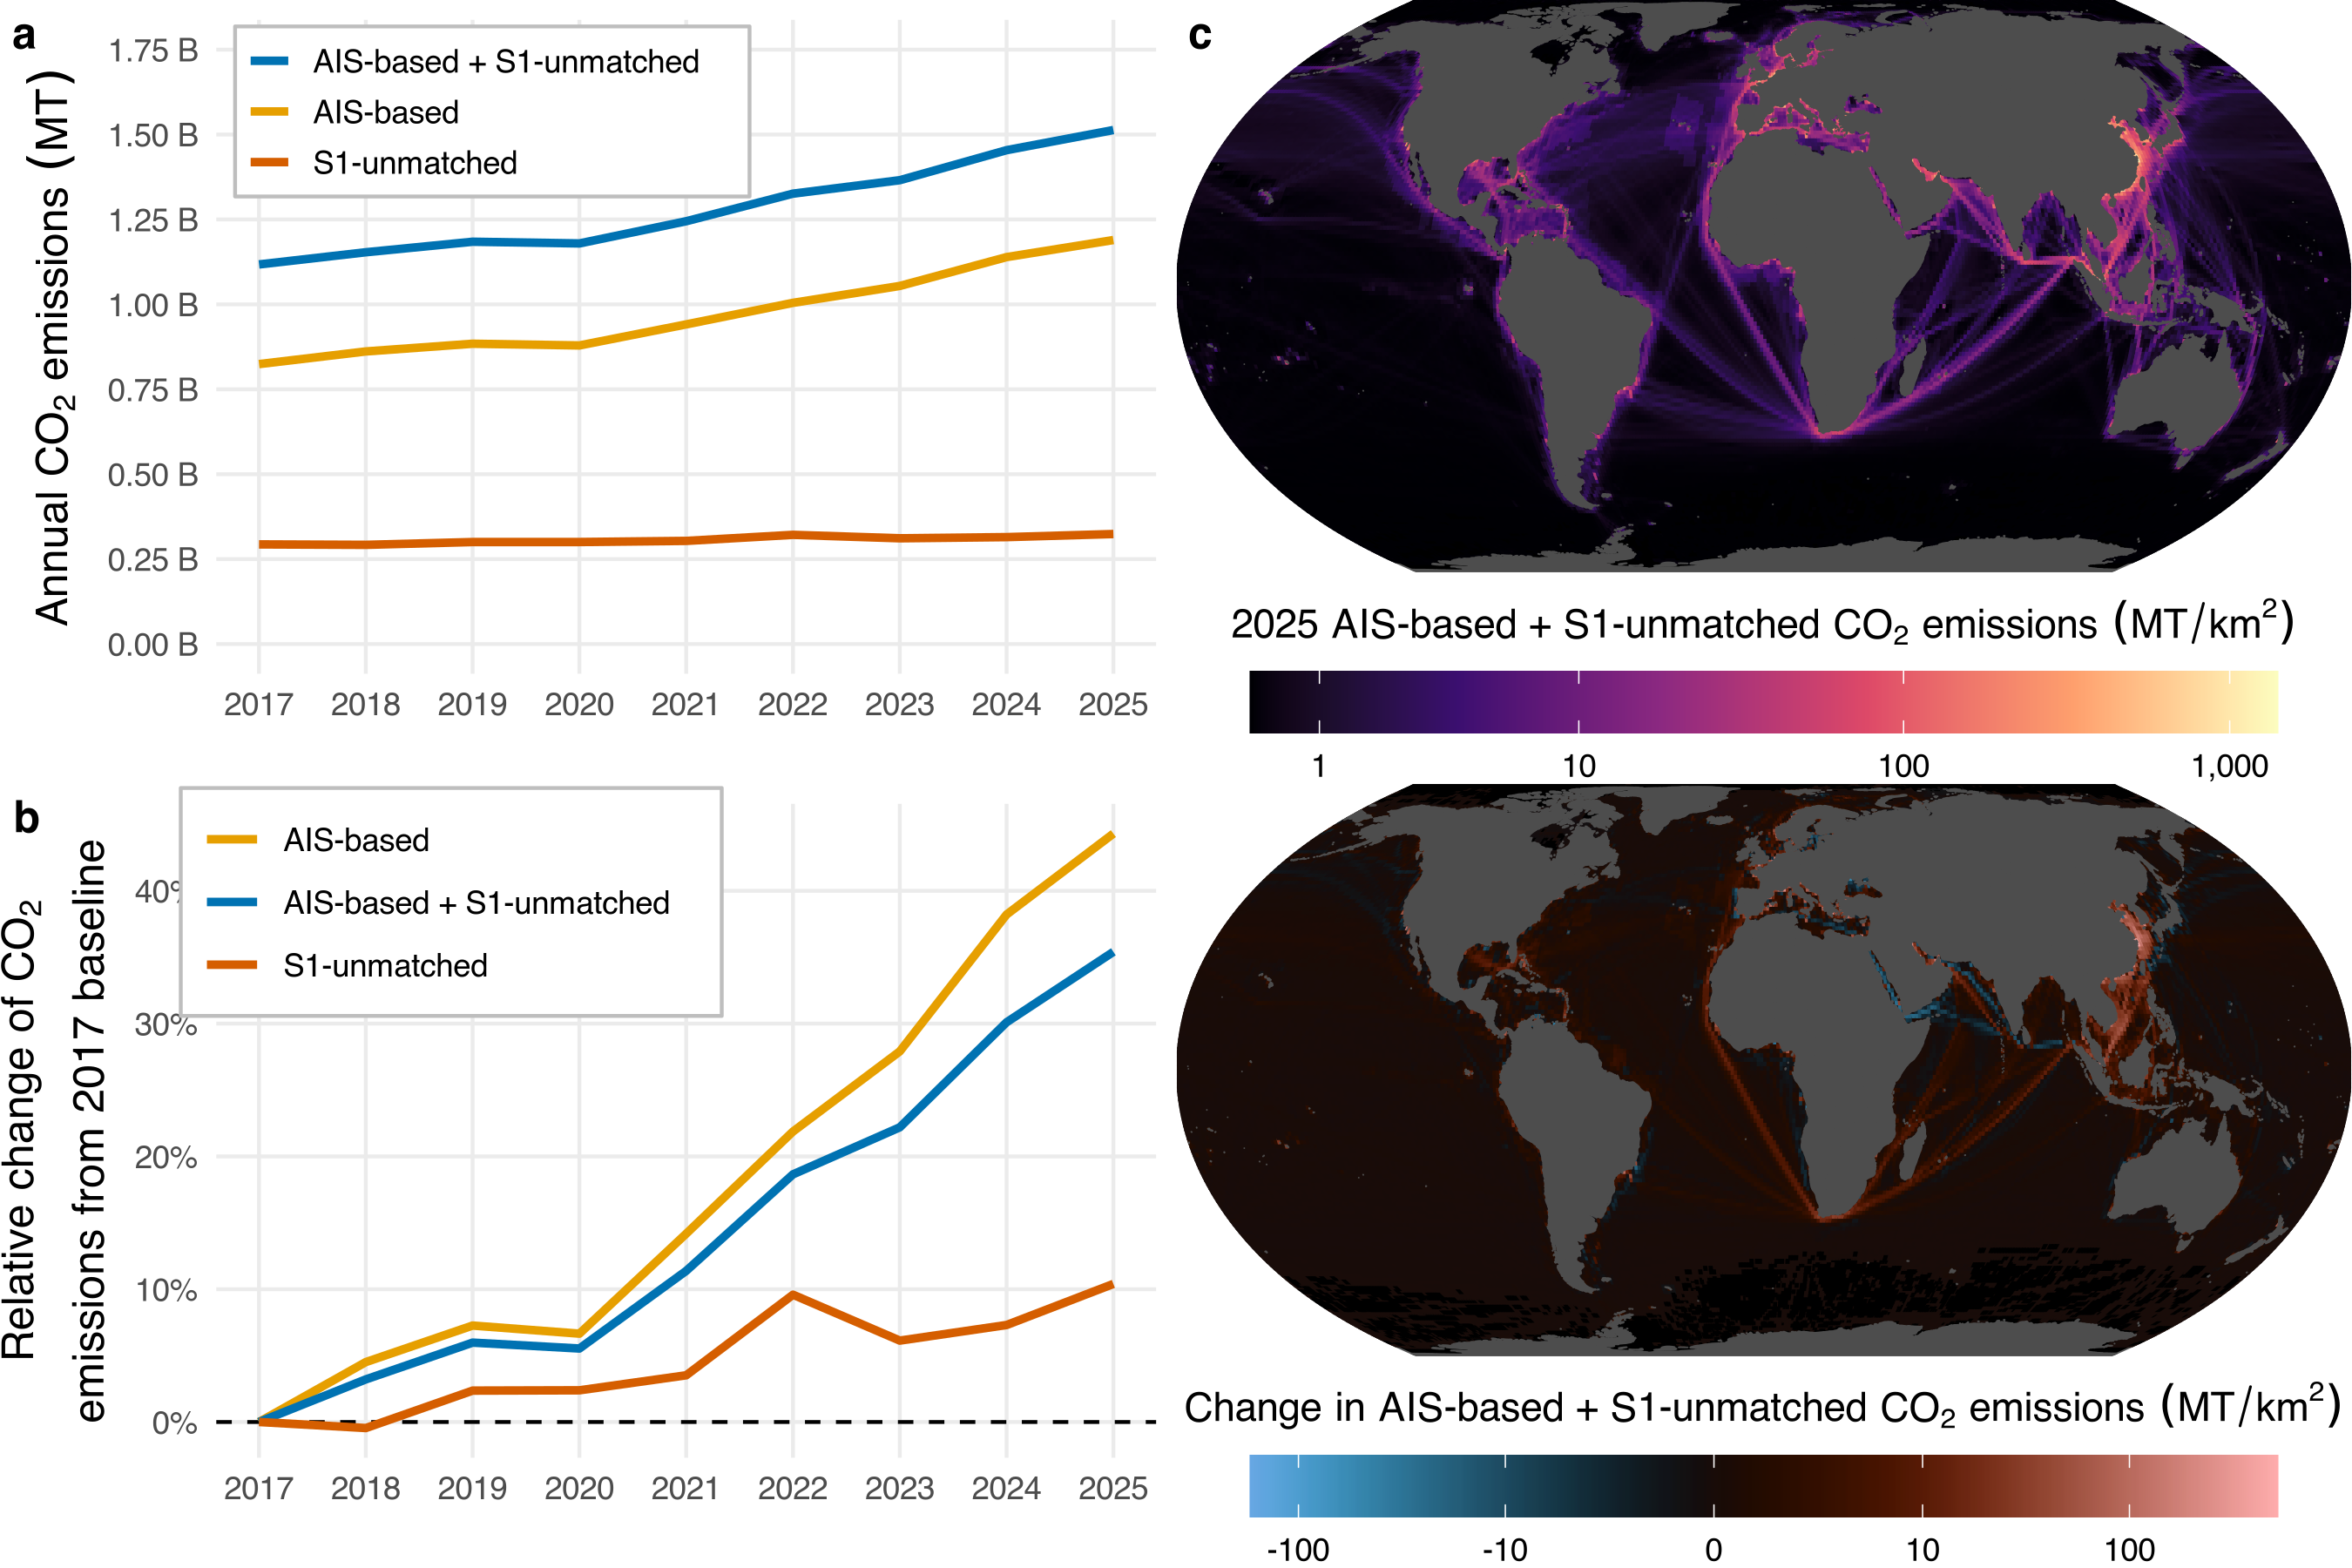
\includegraphics[width=\columnwidth]{figures/fig-emissions-by-data-source-and-maps-1.png}
    \caption{(\DIFdelbeginFL \DIFdelFL{A}\DIFdelendFL \DIFaddbeginFL \DIFaddFL{a}\DIFaddendFL ) Annual marine vessel CO$_{2}$ emissions, with each line colored based on the data source\DIFaddbeginFL \DIFaddFL{: `AIS-based' (emissions from AIS-broadcasting vessels whose AIS signal was received, estimated ping-by-ping from the observed activity of those vessels); `S1-unmatched' (emissions from vessels detected by S1 that could not be matched to an AIS-broadcasting vessel, either because the vessel is completely non-broadcasting or because its AIS signal was not received); and `AIS-based + S1-unmatched' (the aggregation of these `AIS-based' and `S1-unmatched' emissions, our fused total)}\DIFaddendFL . (\DIFdelbeginFL \DIFdelFL{B}\DIFdelendFL \DIFaddbeginFL \DIFaddFL{b}\DIFaddendFL ) Relative change in annual marine vessel CO$_{2}$ emissions from a 2017 baseline, with each line colored based on the data source. (\DIFdelbeginFL \DIFdelFL{C}\DIFdelendFL \DIFaddbeginFL \DIFaddFL{c}\DIFaddendFL ) Spatial map of CO$_{2}$ emissions in \DIFdelbeginFL \DIFdelFL{2024 }\DIFdelendFL \DIFaddbeginFL \DIFaddFL{2025 }\DIFaddendFL (top) and change in CO$_{2}$ emissions between 2017 and \DIFdelbeginFL \DIFdelFL{2024 }\DIFdelendFL \DIFaddbeginFL \DIFaddFL{2025 }\DIFaddendFL (bottom), aggregated across \DIFdelbeginFL \DIFdelFL{AIS-broadcasting vessels }\DIFdelendFL \DIFaddbeginFL \DIFaddFL{AIS-based }\DIFaddendFL and \DIFdelbeginFL \DIFdelFL{non-broadcasting vessels}\DIFdelendFL \DIFaddbeginFL \DIFaddFL{S1-unmatched emissions}\DIFaddendFL , and shown at a 1x1 degree spatial resolution; emissions are area-normalized for each pixel (metric tonnes per square kilometer, shown on a pseudolog-10 scale).}
    \label{fig:fig-emissions-by-data-source-and-maps}
\end{figure}

Estimating \DIFdelbegin \DIFdel{emissions from non-broadcasting vessels not only }\DIFdelend \DIFaddbegin \DIFadd{S1-unmatched emissions }\DIFaddend offers new insights \DIFdelbegin \DIFdel{on the overall magnitude and temporal trends }\DIFdelend \DIFaddbegin \DIFadd{into the temporal trends and spatial patterns }\DIFaddend of global emissions \DIFdelbegin \DIFdel{, but also provides nuanced spatial information and information disaggregated by fishing and non-fishing vessels }\DIFdelend (Fig. \DIFdelbegin \DIFdel{\ref{fig:fig-spatial-temporal-richness-by-fleet-total-pseudolog}). In 2024, 24\% of CO$_{2}$ emissions from fishing vessels were from non-broadcasting vessels, and 14\% of CO$_{2}$ emissions from non-fishing vessels were from non-broadcasting vessels }\DIFdelend \DIFaddbegin \DIFadd{\ref{fig:fig-emissions-time-series-and-maps}). Although total emissions have generally been increasing }\DIFaddend (Fig. \DIFdelbegin \DIFdel{\ref{fig:fig-spatial-temporal-richness-by-fleet-total-pseudolog}A). For both types of vessels, this fraction of emissions from non-broadcasting vessels has been declining steadily since 2020}\DIFdelend \DIFaddbegin \DIFadd{\ref{fig:fig-emissions-time-series-and-maps}a)}\DIFaddend , \DIFaddbegin \DIFadd{the S1-unmatched share of emissions has generally been declining since 2021 (Fig. \ref{fig:fig-emissions-time-series-and-maps}b), }\DIFaddend consistent with a steady increase in AIS monitoring over the period. The time series data reveal strong seasonal trends and event-driven variations in marine GHG emissions. We see consistent dips during major holidays including Christmas, New Year’s Day, and Chinese New Year, as well as during the COVID-19 pandemic (Fig. \DIFdelbegin \DIFdel{\ref{fig:fig-spatial-temporal-richness-by-fleet-total-pseudolog}A and }\DIFdelend \DIFaddbegin \DIFadd{\ref{fig:fig-emissions-time-series-and-maps}a and Supplementary }\DIFaddend Fig. \ref{fig:fig-pollutant-time-series}). Being able to spatially quantify \DIFdelbegin \DIFdel{emissions from non-broadcasting vessels }\DIFdelend \DIFaddbegin \DIFadd{S1-unmatched emissions }\DIFaddend fills important gaps in our current understanding of where marine vessel emissions take place, \DIFdelbegin \DIFdel{particularly in southeast Asia, China, the Caribbean}\DIFdelend \DIFaddbegin \DIFadd{with large concentrations of these previously untracked emissions in East and Southeast Asia, the Mediterranean}\DIFaddend , and the \DIFdelbegin \DIFdel{Mediterranean }\DIFdelend \DIFaddbegin \DIFadd{Caribbean }\DIFaddend (Fig. \DIFdelbegin \DIFdel{\ref{fig:fig-spatial-temporal-richness-by-fleet-total-pseudolog}B}\DIFdelend \DIFaddbegin \DIFadd{\ref{fig:fig-emissions-time-series-and-maps}c, middle map}\DIFaddend ), crucial for targeting policy or private sector interventions. \DIFaddbegin \DIFadd{Expressed as a share of each pixel's total emissions, the pattern is clearer (Fig. \ref{fig:fig-emissions-time-series-and-maps}c, bottom map): the S1-unmatched contribution is concentrated mostly in coastal waters, with the highest shares in Southeast Asia, the Caribbean, and the Mediterranean. In the major open-ocean shipping lanes, where large AIS-broadcasting vessels dominate, the share is close to zero. Our dataset also provides this sort of nuanced spatiotemporal information disaggregated by fishing and non-fishing vessels (Supplementary Fig. \ref{fig:fig-spatial-temporal-richness-by-fleet-total-pseudolog}). In 2025, 35\% of CO$_{2}$ emissions from fishing vessels were from S1-unmatched detections, and 16\% of CO$_{2}$ emissions from non-fishing vessels were from S1-unmatched detections.
}\DIFaddend 

\begin{figure}[H]
    \centering
    \DIFdelbeginFL %DIFDELCMD < 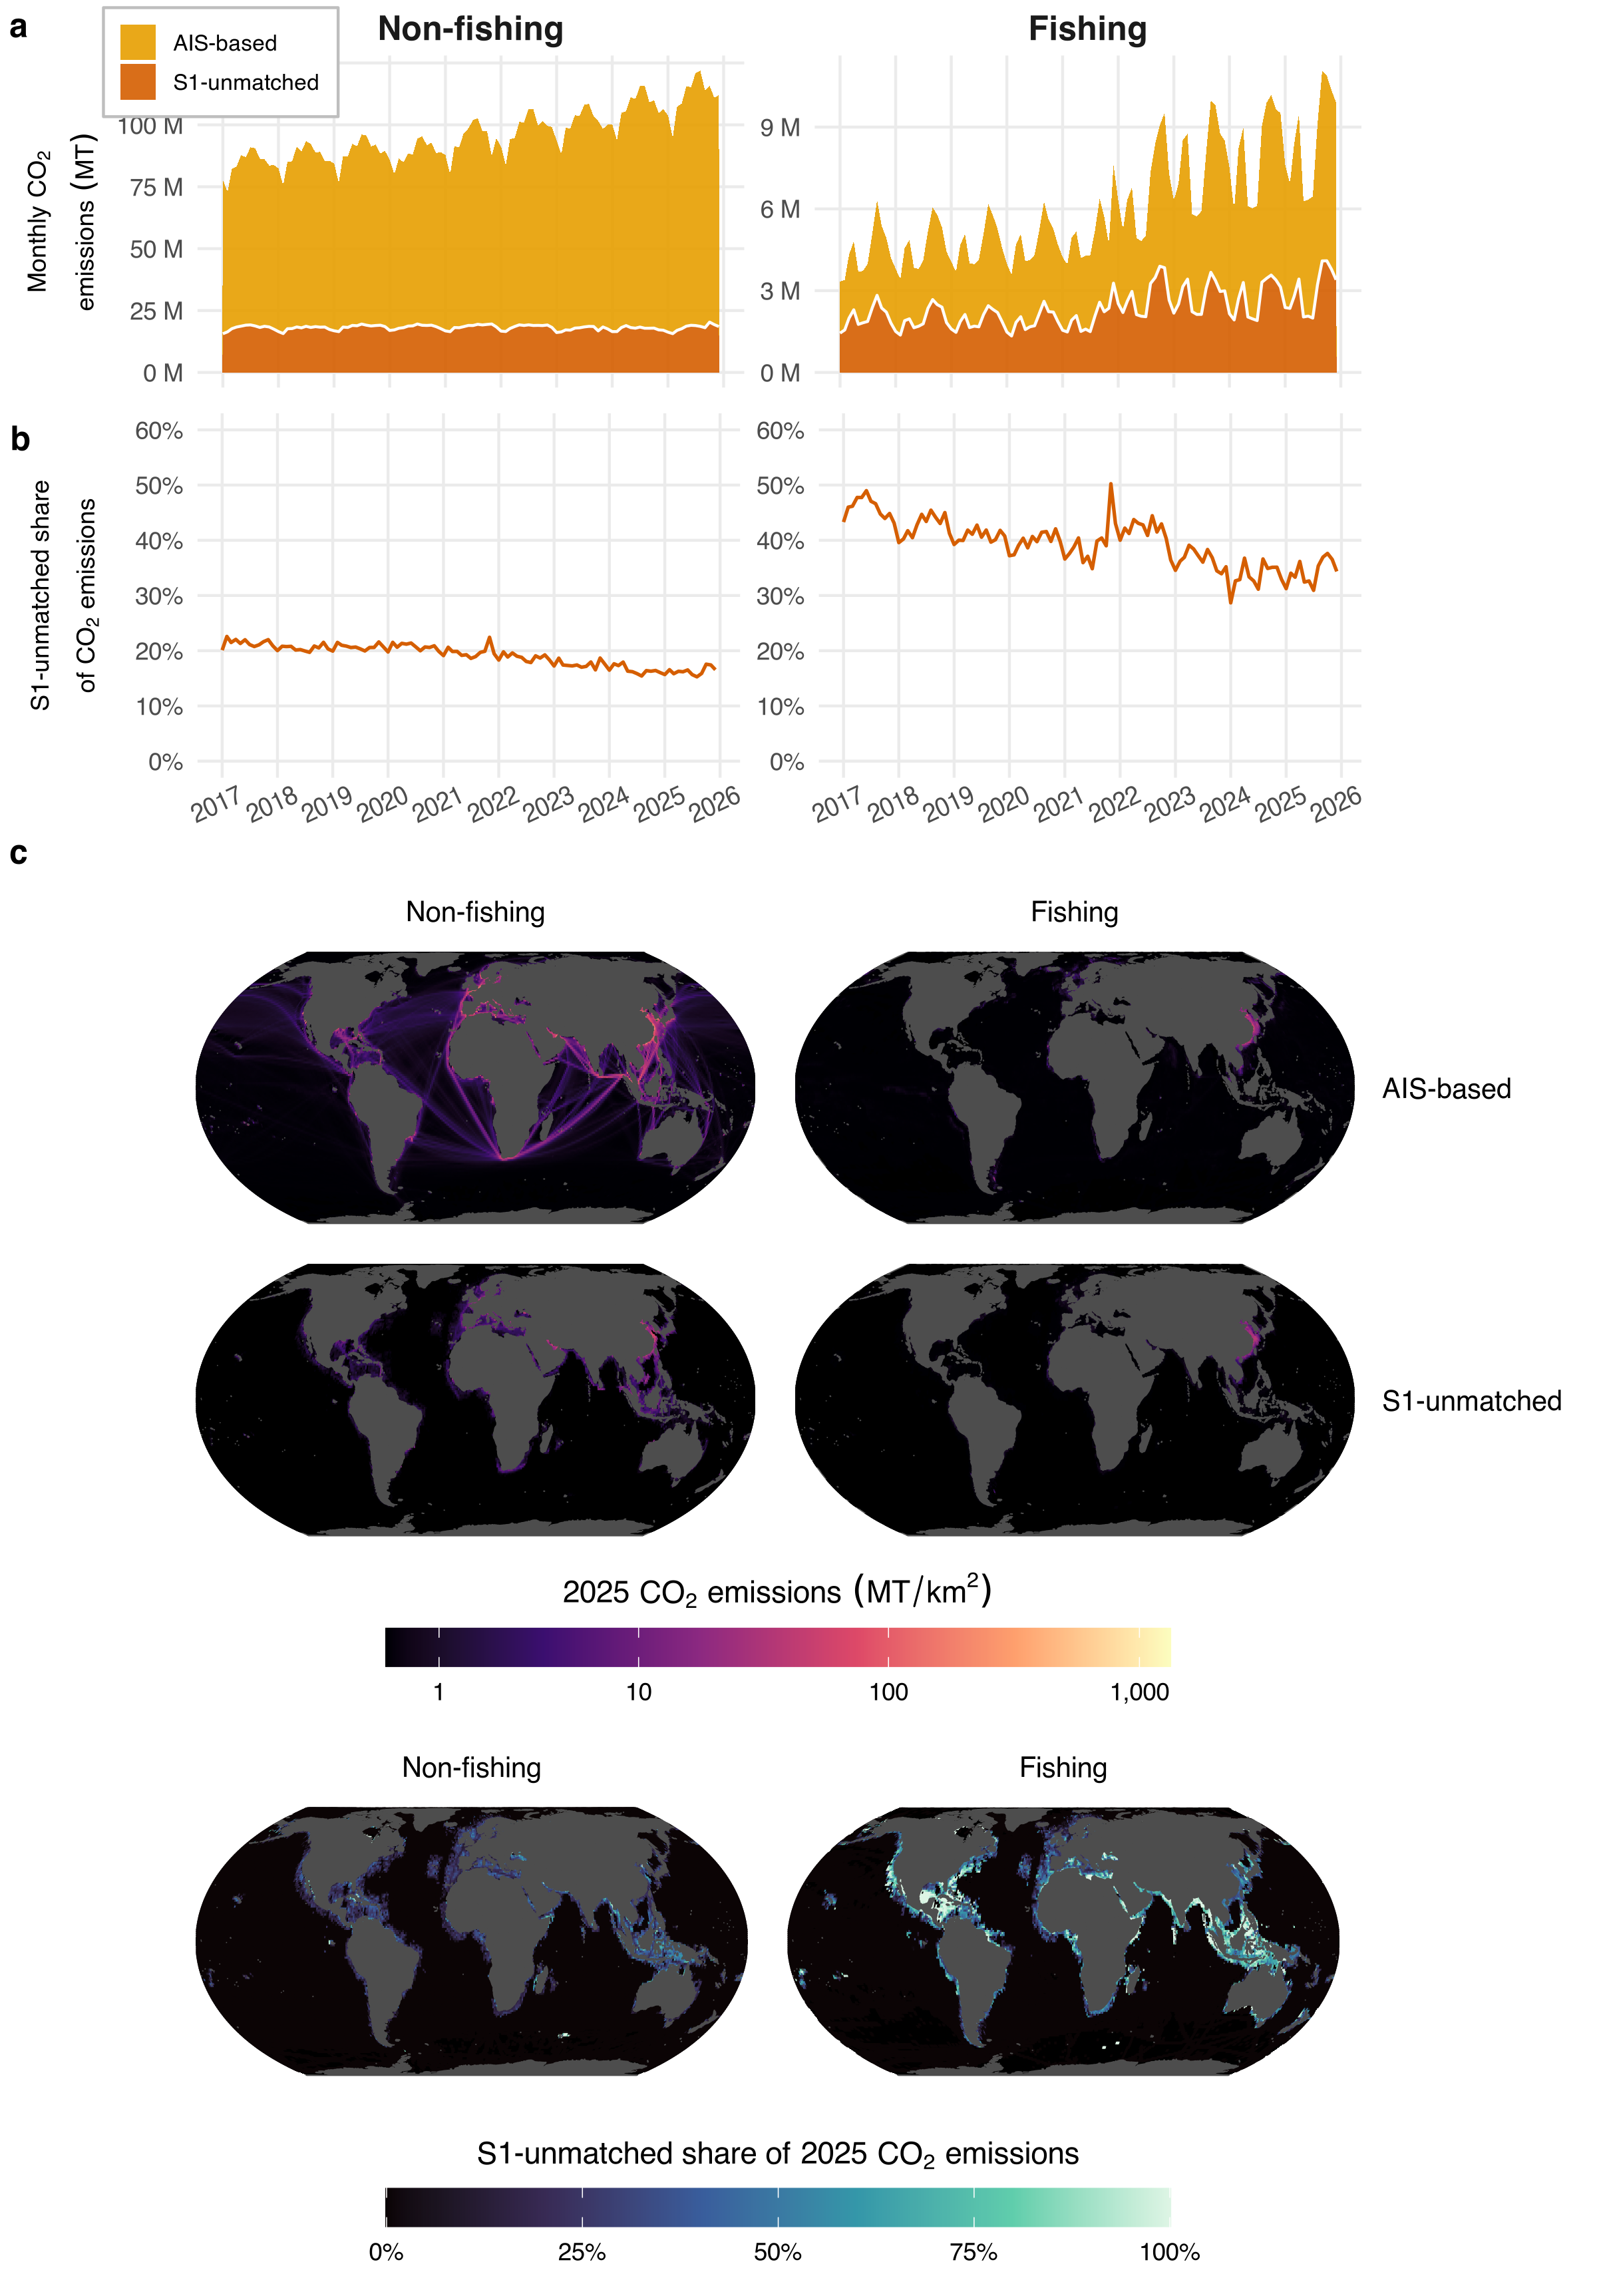
\includegraphics[width=\columnwidth]{figures/fig-spatial-temporal-richness-by-fleet-total-pseudolog-1.png}
%DIFDELCMD <     %%%
\DIFdelendFL \DIFaddbeginFL 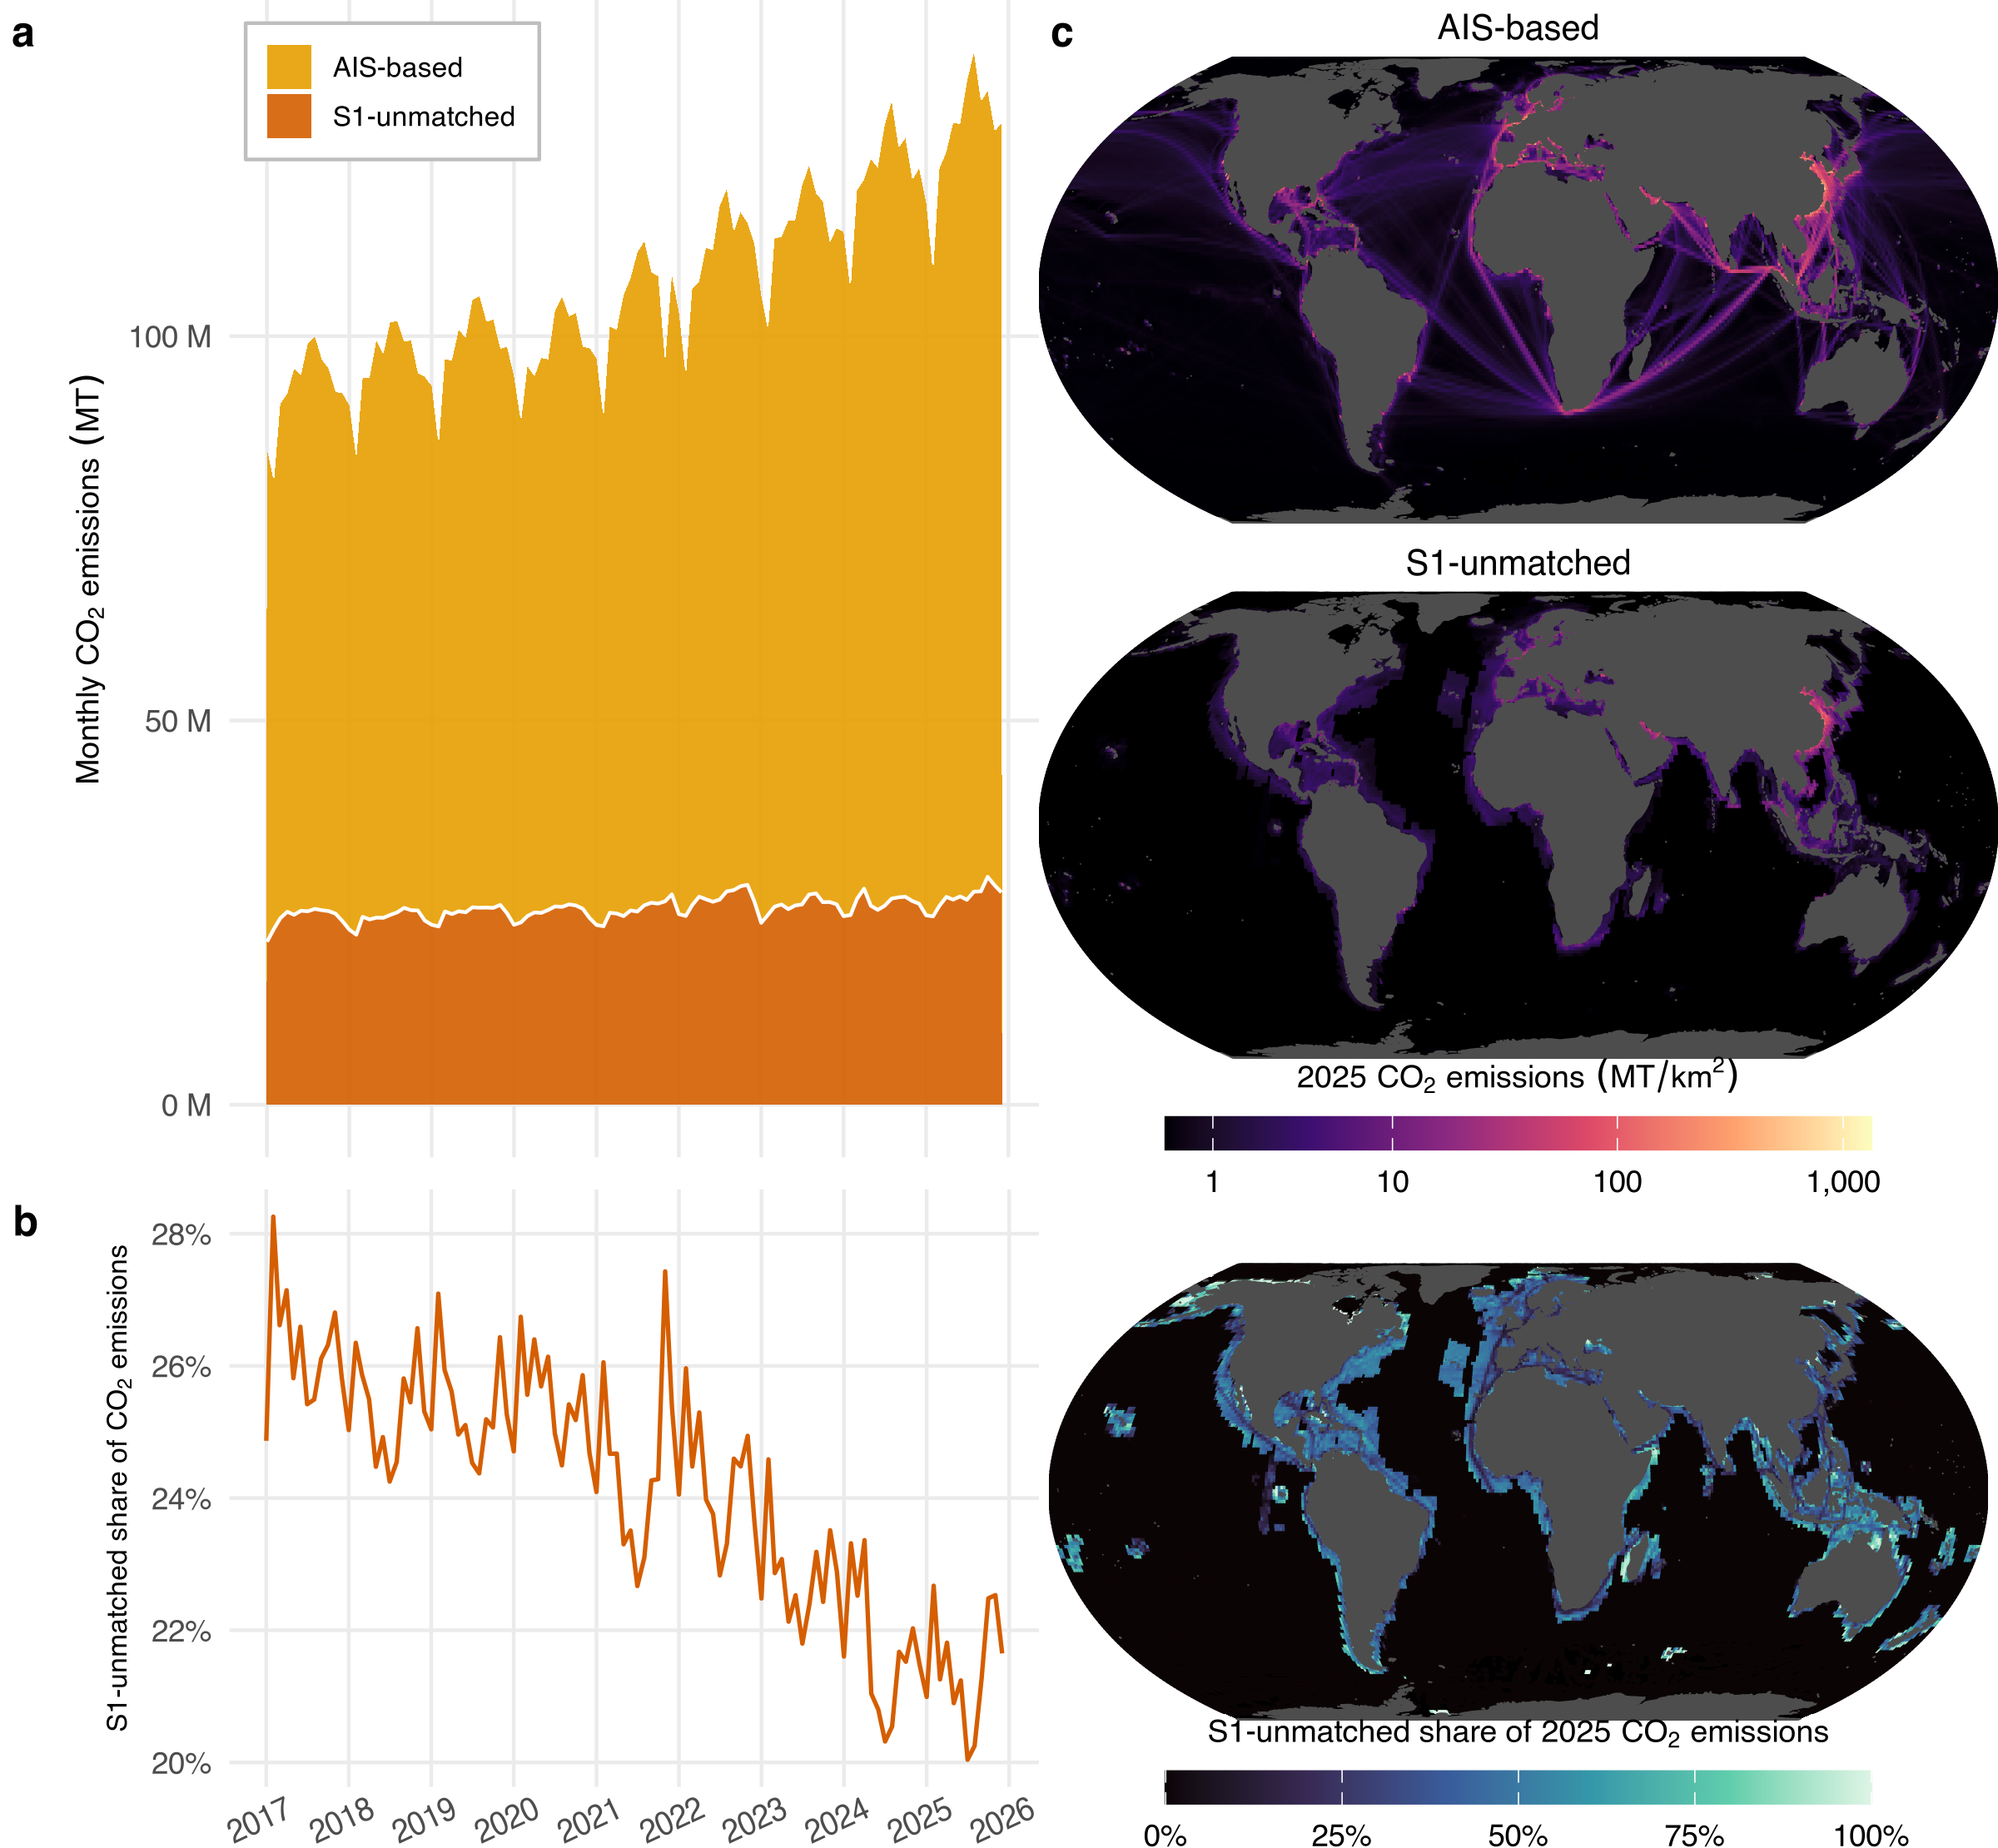
\includegraphics[width=\columnwidth]{figures/fig-emissions-time-series-and-maps-1.png}
    \DIFaddendFL \caption{(\DIFdelbeginFL \DIFdelFL{A}\DIFdelendFL \DIFaddbeginFL \DIFaddFL{a}\DIFaddendFL ) Time series of monthly global CO$_2$ emissions, \DIFdelbeginFL \DIFdelFL{shown for both }\DIFdelendFL \DIFaddbeginFL \DIFaddFL{stacked by data source: `AIS-based' (emissions from }\DIFaddendFL AIS-broadcasting \DIFdelbeginFL \DIFdelFL{and S1-detected non-broadcasting }\DIFdelendFL vessels \DIFaddbeginFL \DIFaddFL{whose AIS signal was received}\DIFaddendFL , \DIFdelbeginFL \DIFdelFL{and for both fishing and non-fishing }\DIFdelendFL \DIFaddbeginFL \DIFaddFL{estimated ping-by-ping from the observed activity of those }\DIFaddendFL vessels\DIFaddbeginFL \DIFaddFL{); `S1-unmatched' (emissions from vessels detected by S1 that could not be matched to an AIS-broadcasting vessel, either because the vessel is completely non-broadcasting or because its AIS signal was not received); the top of the stack is their sum, our fused total (`AIS-based + S1-unmatched')}\DIFaddendFL . (\DIFdelbeginFL \DIFdelFL{B}\DIFdelendFL \DIFaddbeginFL \DIFaddFL{b}\DIFaddendFL ) \DIFaddbeginFL \DIFaddFL{Time series of the monthly share of global CO$_{2}$ emissions attributable to S1-detected unmatched vessels. (c) }\DIFaddendFL Spatial distribution of \DIFdelbeginFL \DIFdelFL{cumulative 2017-2024 }\DIFdelendFL \DIFaddbeginFL \DIFaddFL{2025 }\DIFaddendFL CO$_{2}$ emissions from \DIFdelbeginFL \DIFdelFL{both }\DIFdelendFL AIS-broadcasting \DIFaddbeginFL \DIFaddFL{vessels (top) }\DIFaddendFL and S1-detected \DIFdelbeginFL \DIFdelFL{non-broadcasting }\DIFdelendFL \DIFaddbeginFL \DIFaddFL{unmatched }\DIFaddendFL vessels \DIFaddbeginFL \DIFaddFL{(middle)}\DIFaddendFL , \DIFdelbeginFL \DIFdelFL{for both fishing and non-fishing vessels, and }\DIFdelendFL shown at a 1x1 degree spatial resolution; emissions are area-normalized for each pixel (metric tonnes per square kilometer, shown on a pseudolog-10 scale). \DIFaddbeginFL \DIFaddFL{The bottom map shows, for each pixel, the share of its 2025 CO$_{2}$ emissions that is S1-unmatched. Because this is a bounded percentage rather than a magnitude, it carries its own color scale, distinct from the one shared by the two maps above it. Every pixel carries a modeled value, so a pixel reading 0\% is one with no S1-unmatched emissions rather than one with no data. Note that panel b and the bottom map of panel c show the same quantity, in time and in space respectively, and that panel b's vertical axis does not start at zero. The spike in panel b in November 2021 reflects a one-month drop in AIS-based emissions, coinciding with the blackout of terrestrial AIS in Chinese waters (Supplementary Note \ref{sec:ais-receiver-types}), rather than a change in S1-unmatched emissions.}\DIFaddendFL }
    \DIFdelbeginFL %DIFDELCMD < \label{fig:fig-spatial-temporal-richness-by-fleet-total-pseudolog}
%DIFDELCMD < %%%
\DIFdelendFL \DIFaddbeginFL \label{fig:fig-emissions-time-series-and-maps}
\DIFaddendFL \end{figure}

Across the entire 2017 to \DIFdelbegin \DIFdel{2024 }\DIFdelend \DIFaddbegin \DIFadd{2025 }\DIFaddend time series, almost all \DIFdelbegin \DIFdel{non-broadcasting emissions (95.3}\DIFdelend \DIFaddbegin \DIFadd{S1-unmatched emissions (95.7}\DIFaddend \%) occurred inside the S1 footprint and in pixel-months that were imaged by S1 (Fig. \ref{fig:fig-spatial-coverage-footprint}). This makes sense because part of the Copernicus system's observation strategy for S1 is specifically focused on imaging coastal and shipping areas, where ship density is highest \cite{ESA2013S1Handbook}. Our machine learning model for predicting these emissions directly from observed S1 detection density achieves a high out-of-sample predictive performance (traditional R$^{2}$ = \DIFdelbegin \DIFdel{0.96 }\DIFdelend \DIFaddbegin \DIFadd{0.94 }\DIFaddend and total percent error of \DIFdelbegin \DIFdel{-7.4}\DIFdelend \DIFaddbegin \DIFadd{-7.8}\DIFaddend \% for CO$_2$, Table \ref{tab:all_performance_metrics_table}). Only \DIFdelbegin \DIFdel{4.6\% of non-broadcasting }\DIFdelend \DIFaddbegin \DIFadd{4.2\% of S1-unmatched }\DIFaddend emissions occurred inside the S1 footprint but in pixel-months that weren't imaged by S1, requiring us to use a two-stage hurdle framework using both a classification model (F1 Score = \DIFdelbegin \DIFdel{0.73}\DIFdelend \DIFaddbegin \DIFadd{0.72}\DIFaddend ) and a regression model (traditional R$^{2}$ = \DIFdelbegin \DIFdel{0.70}\DIFdelend \DIFaddbegin \DIFadd{0.68}\DIFaddend ) to predict S1 detection density before predicting emissions (traditional R$^{2}$ = \DIFdelbegin \DIFdel{0.96}\DIFdelend \DIFaddbegin \DIFadd{0.94}\DIFaddend ). Only \DIFdelbegin \DIFdel{0.1\% of non-broadcasting }\DIFdelend \DIFaddbegin \DIFadd{0.070\% of S1-unmatched }\DIFaddend emissions occurred outside the S1 footprint entirely, since most vessels operating in these open ocean areas use AIS.

Our vessel-level \DIFdelbegin \DIFdel{AIS-broadcasting }\DIFdelend \DIFaddbegin \DIFadd{AIS-based }\DIFaddend emissions data provide a detailed understanding of marine vessel emissions across vessel classes and activity types (Fig. \ref{fig:fig-ais-data-richness}). \DIFdelbegin \DIFdel{Chemical and oil tankers, some of which }\DIFdelend \DIFaddbegin \DIFadd{We are able to distinguish activity between 37 classes of vessels, including 14 classes of fishing vessels; this makes our inventory the first to our knowledge that provides this level of emissions detail for fishing vessels. Container and bulk carriers, which transport much of the world's goods by sea, are the highest-emitting cargo classes (Fig. \ref{fig:fig-ais-data-richness}a). Oil tankers, which themselves }\DIFaddend transport fossil fuels\DIFdelbegin \DIFdel{including crude oil, are themselves the largest emitters (Fig. \ref{fig:fig-ais-data-richness}A). }\DIFdelend \DIFaddbegin \DIFadd{, are the highest-emitting tanker type. These vessel classes are ranked similarly in other inventories \mbox{%DIFAUXCMD
\cite{johanssonGlobalAssessmentShipping2017, kramelGlobalShippingEmissions2021, yiHighresolutionGlobalShipping2025, mao2025greenhouse}}\hskip0pt%DIFAUXCMD
, with the notable exception of the passenger category. Passenger vessels have a highly aggregated definition in our model, composed of several diverse vessel subclasses including ferries, cruise ships, Ro-Pax, and yachts, which makes this category the most numerous class in our fleet and consequently the largest emitting group in 2025 (Supplementary Fig. \ref{fig:figS-fleet-sankey-with-series-2025}). This also in part reflects our broader vessel coverage compared to other inventories, since we include many smaller vessels that are absent or underrepresented elsewhere: vessels below 25 m account for most passenger emissions in our inventory (Supplementary Fig. \ref{fig:figS-passenger-size-panels}, panel b), and fishing vessels are our second-largest class by vessel count (Supplementary Fig. \ref{fig:figS-fleet-sankey-with-series-2025}). }\DIFaddend Trawlers, which use an energy-intensive fishing technique in which nets are dragged through the water \cite{coello2015ais}, are the highest-emitting type of fishing vessel. Emissions from AIS-broadcasting vessels can \DIFaddbegin \DIFadd{also }\DIFaddend be assigned to port stays in particular countries and port-to-port voyages within- and between-countries by analyzing the movement tracks of each individual vessel (Fig. \ref{fig:fig-ais-data-richness}\DIFdelbegin \DIFdel{A-B}\DIFdelend \DIFaddbegin \DIFadd{c and Supplementary Fig. \ref{fig:fig-emissions-by-country-and-activity-type}}\DIFaddend ). Most emissions for \DIFdelbegin \DIFdel{non-fishing }\DIFdelend \DIFaddbegin \DIFadd{cargo and tanker }\DIFaddend vessels occur during international trips, while most \DIFdelbegin \DIFdel{emissions for fishing vessels occur during domestic trips. China, United States, and Japan }\DIFdelend \DIFaddbegin \DIFadd{service and passenger vessel emissions occur within ports (Fig. \ref{fig:fig-ais-data-richness}c). China, Japan, and the United States }\DIFaddend had the most CO$_{2}$ emissions during within-country domestic trips in \DIFdelbegin \DIFdel{2024. }\DIFdelend \DIFaddbegin \DIFadd{2025. }\DIFaddend China, Malaysia, and \DIFaddbegin \DIFadd{the }\DIFaddend United States had the most CO$_{2}$ emissions during international trips that started or ended in these countries in \DIFdelbegin \DIFdel{2024 }\DIFdelend \DIFaddbegin \DIFadd{2025 }\DIFaddend (where the emissions from each trip are partitioned equally to its departure and arrival country). China, \DIFaddbegin \DIFadd{the }\DIFaddend United States, and \DIFdelbegin \DIFdel{South Korea }\DIFdelend \DIFaddbegin \DIFadd{Indonesia }\DIFaddend had the most CO$_{2}$ emissions during port stays. \DIFaddbegin \DIFadd{Country totals for every activity type are summarized in Supplementary Fig. \ref{fig:fig-emissions-by-country-and-activity-type} and listed in Supplementary Table \ref{tab:top_countries_by_activity_type}. We note that roughly 5\% of AIS messages are attributable to AIS transponders that are not on vessels, but are rather on buoys, fish aggregating devices (FADs), navigation aids, offshore structures, fishing gear, and other objects. Transponders that our vessel class model identifies as non-vessels are excluded from our analysis.
}\DIFaddend 


 \begin{figure}[H]
    \centering
    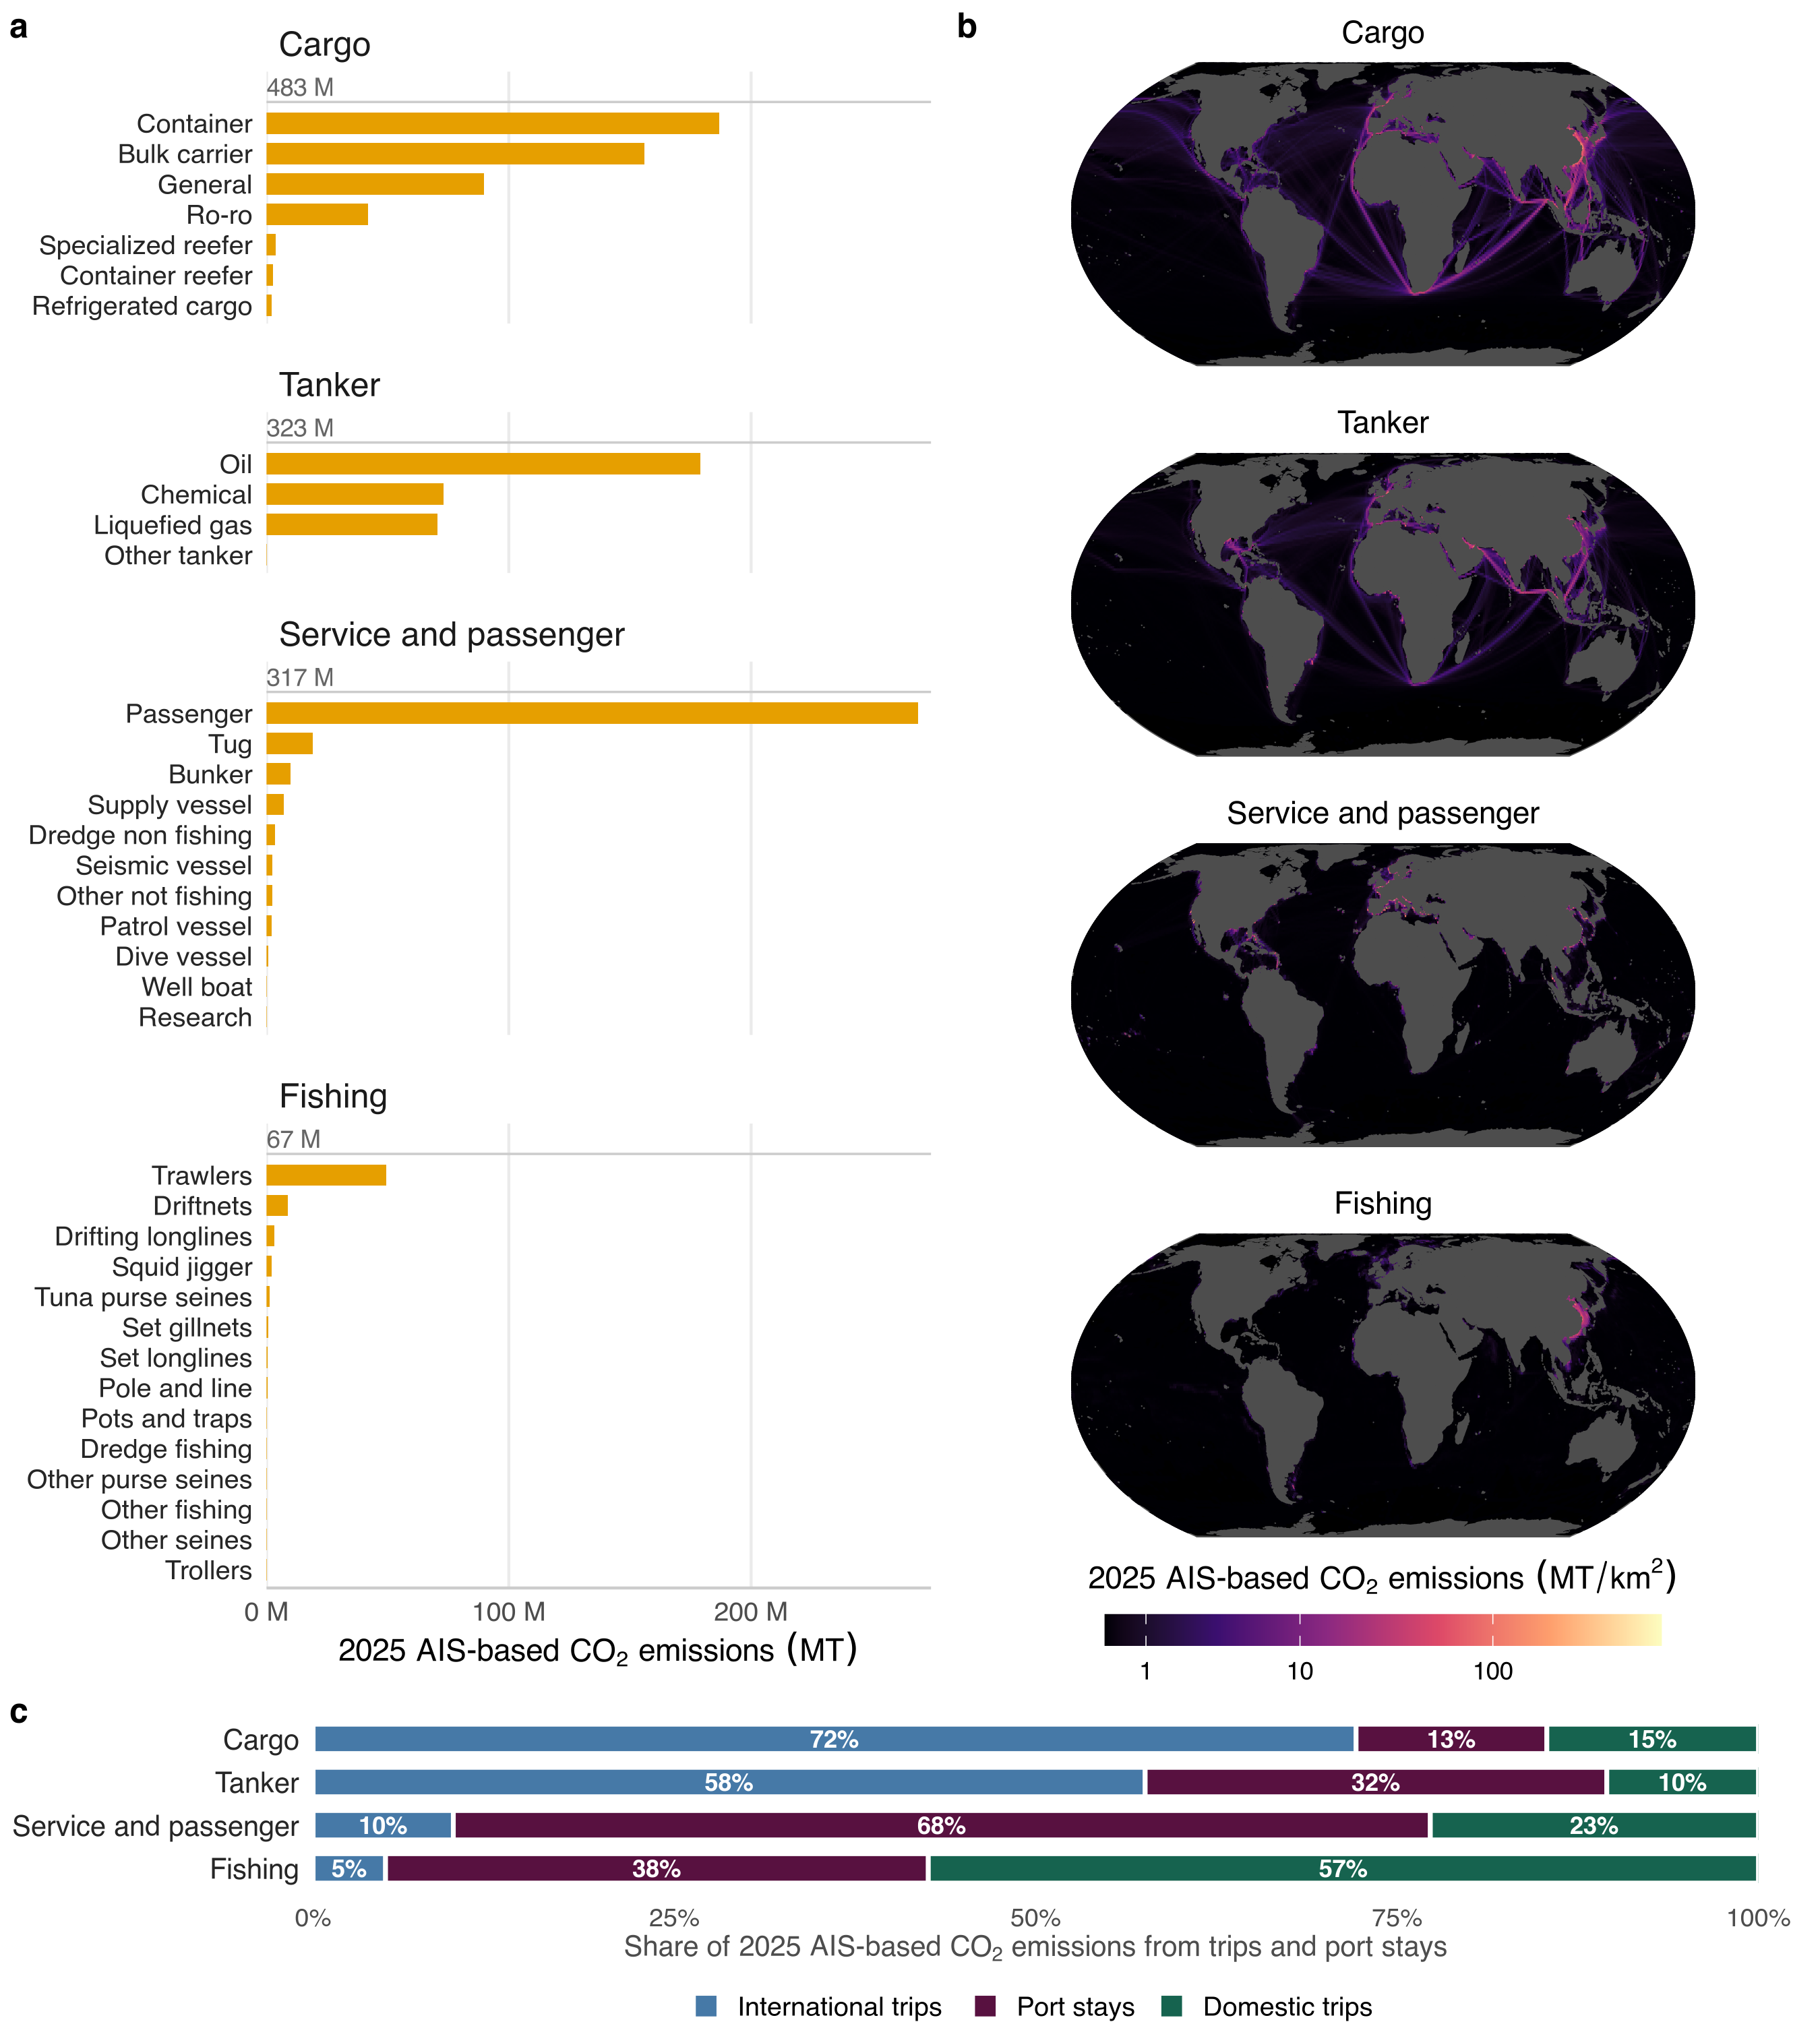
\includegraphics[width=\columnwidth]{figures/fig-ais-data-richness-1.png}
    \caption{Richness of AIS-broadcasting vessel emissions data \DIFaddbeginFL \DIFaddFL{(AIS-based emissions only; S1-unmatched emissions are not included)}\DIFaddendFL , showing: (\DIFdelbeginFL \DIFdelFL{A}\DIFdelendFL \DIFaddbeginFL \DIFaddFL{a}\DIFaddendFL ) \DIFaddbeginFL \DIFaddFL{Total 2025 }\DIFaddendFL CO$_{2}$ emissions by vessel \DIFdelbeginFL \DIFdelFL{type }\DIFdelendFL \DIFaddbeginFL \DIFaddFL{class }\DIFaddendFL for AIS-broadcasting vessels\DIFdelbeginFL \DIFdelFL{during different activity types (international trips}\DIFdelendFL \DIFaddbeginFL \DIFaddFL{. Vessel classes are grouped into four families}\DIFaddendFL , \DIFdelbeginFL \DIFdelFL{port stays}\DIFdelendFL \DIFaddbeginFL \DIFaddFL{with the total for each family shown above its bars; every class in a family is shown as its own bar}\DIFaddendFL , \DIFdelbeginFL \DIFdelFL{and domestic trips), }\DIFdelendFL \DIFaddbeginFL \DIFaddFL{so panel heights differ with the number of classes. These totals are }\DIFaddendFL aggregated \DIFdelbeginFL \DIFdelFL{for activities ending }\DIFdelendFL \DIFaddbeginFL \DIFaddFL{from the same gridded emissions shown }\DIFaddendFL in \DIFdelbeginFL \DIFdelFL{2024. }\DIFdelendFL \DIFaddbeginFL \DIFaddFL{panel b, so the two panels describe exactly the same emissions and the bars sum to the mapped total. }\DIFaddendFL (\DIFdelbeginFL \DIFdelFL{B}\DIFdelendFL \DIFaddbeginFL \DIFaddFL{b}\DIFaddendFL ) \DIFaddbeginFL \DIFaddFL{Spatial distribution of 2025 }\DIFaddendFL CO$_{2}$ emissions \DIFdelbeginFL \DIFdelFL{by country for }\DIFdelendFL \DIFaddbeginFL \DIFaddFL{from }\DIFaddendFL AIS-broadcasting vessels \DIFdelbeginFL \DIFdelFL{during  during different activity types }\DIFdelendFL \DIFaddbeginFL \DIFaddFL{for each of those same vessel class families, shown at a 1x1 degree spatial resolution; emissions are area-normalized for each pixel }\DIFaddendFL (\DIFaddbeginFL \DIFaddFL{metric tonnes per square kilometer, shown on a pseudolog-10 scale). Families appear in the same order in both panels. (c) For each family, the share of CO$_{2}$ emissions attributable to }\DIFaddendFL international trips, port stays, and domestic trips \DIFdelbeginFL \DIFdelFL{), aggregated for activities ending in 2024. For both panels, }\DIFdelendFL \DIFaddbeginFL \DIFaddFL{(note that panel c is not a decomposition of panel a: it covers only }\DIFaddendFL emissions \DIFdelbeginFL \DIFdelFL{for each international }\DIFdelendFL \DIFaddbeginFL \DIFaddFL{that could be assigned to a }\DIFaddendFL trip \DIFdelbeginFL \DIFdelFL{are partitioned equally }\DIFdelendFL \DIFaddbeginFL \DIFaddFL{or port visit that ended in 2025; each family sums }\DIFaddendFL to \DIFaddbeginFL \DIFaddFL{100\% of }\DIFaddendFL its \DIFdelbeginFL \DIFdelFL{departure and arrival country}\DIFdelendFL \DIFaddbeginFL \DIFaddFL{own assigned emissions}\DIFaddendFL ).\DIFdelbeginFL \DIFdelFL{Countries with no values are shown in black.}\DIFdelendFL }
    \label{fig:fig-ais-data-richness}
\end{figure}

\DIFdelbegin \DIFdel{Our novel }\DIFdelend \DIFaddbegin \DIFadd{By developing new }\DIFaddend methods for inferring key missing vessel characteristics that are necessary for AIS-based emissions modeling\DIFdelbegin \DIFdel{allow us to }\DIFdelend \DIFaddbegin \DIFadd{, we can }\DIFaddend accurately estimate vessel-level emissions for a huge swath of the world's fleet that does not otherwise have \DIFdelbegin \DIFdel{publicly available }\DIFdelend \DIFaddbegin \DIFadd{the necessary }\DIFaddend vessel characteristic information \DIFaddbegin \DIFadd{in public registries}\DIFaddend . Of the roughly \DIFdelbegin \DIFdel{880}\DIFdelend \DIFaddbegin \DIFadd{775}\DIFaddend ,000 AIS-broadcasting vessels in our analysis \DIFaddbegin \DIFadd{(every vessel emitting at any point during our 2017--2025 study period), we matched 139,000 (18\%) to public registries or proprietary databases, the majority of which (93,400) were IMO-registered. However, the vast majority of AIS-broadcasting vessels were not matched to these registries, meaning that we needed to use model-derived vessel characteristics for between 83\% and nearly 100\% of vessels, depending on the characteristic (Table \ref{tab:characteristic-availability}). Registry coverage is weakest among small vessels: in 2017}\DIFaddend , \DIFdelbegin \DIFdel{only 89,600 (10\%) are registered with the IMO,while 55, 600 (6\% ) are listed }\DIFdelend \DIFaddbegin \DIFadd{80\% of AIS-broadcasting vessels under 50 m had no registry match, against 7\% of those 150 m and over. Those small vessels are also the fastest-growing part of our AIS-based inventory, rising from 17\% of AIS-based CO$_{2}$ in 2017 to 27\% in 2025, so accurate inference of missing vessel characteristics becomes increasingly important over time. Because many large vessels are already listed with the IMO, 39\% of our 2017--2025 AIS-based CO$_{2}$ emissions come from these vessels; 19\% come from vessels listed on other registries; and 42\% come from vessels not matched to any registry, whose emissions rest entirely }\DIFaddend on \DIFdelbegin \DIFdel{some other public registry; this leaves over 735,000 vessels (84\% ) that have no public registryinformation and must rely completely on }\DIFdelend modeled vessel characteristics\DIFdelbegin \DIFdel{(main engine power and design speed).
Using the main engine power and design speed }\DIFdelend \DIFaddbegin \DIFadd{.
}

\DIFadd{Using the vessel characteristic }\DIFaddend values that are derived from our machine learning models, we achieve an out-of-sample model performance of \DIFdelbegin \DIFdel{0.82 }\DIFdelend \DIFaddbegin \DIFadd{0.85 }\DIFaddend traditional R$^{2}$ when comparing our daily vessel-specific CO$_{2}$ emissions estimates against those derived from a proprietary vessel registry dataset \DIFdelbegin \DIFdel{of over 15}\DIFdelend \DIFaddbegin \DIFadd{(S\&P Global Market Intelligence's Ships Dataset) of over 16}\DIFaddend ,000 vessel-specific fuel consumption values that were measured during at-sea trials (Fig. \ref{fig:fig-registered-data-performance}). If we were to instead estimate emissions with our model using only currently available public vessel characteristic data (i.e., the IMO provides lookup tables for average main engine power and design speed for different vessel types and sizes \cite{fourth2020greenhouse}), we would only achieve a predict\DIFaddbegin \DIFadd{ive}\DIFaddend  performance value of \DIFdelbegin \DIFdel{0.74 }\DIFdelend \DIFaddbegin \DIFadd{0.73 }\DIFaddend traditional R$^{2}$. We also measured the performance of our model's ability to estimate annual vessel-level CO$_{2}$ emissions estimates by comparing our estimates to those available in the publicly available European Maritime Safety Agency’s Monitoring, Reporting, and Verification (MRV) database \cite{mrv_emissions}. Using a set of over 2\DIFaddbegin \DIFadd{7}\DIFaddend  ,000 matched vessel-specific annual emissions estimates, we found a performance value of \DIFdelbegin \DIFdel{0.81 }\DIFdelend \DIFaddbegin \DIFadd{0.84 }\DIFaddend traditional R$^{2}$ (Table \ref{tab:tab-performance-tolerance-table}).
\DIFdelbegin \DIFdel{Because many large vessels are already registered with the IMO, the majority of our total CO$_2$ emissions come from these vessels (61\%); 4\% come from vessels listed on other registries; and 35\% come from vessels with no public registry information and which rely entirely on modeled vessel characteristics.
}\DIFdelend 

The dataset also allows us to examine large-scale trends in marine vessel emissions for different parts of the ocean, and for different sectors of the global economy. Although vessel activity in the Southern Ocean represents a very small fraction\DIFdelbegin \DIFdel{s}\DIFdelend  of the world's marine vessel emissions (\DIFdelbegin \DIFdel{0.05}\DIFdelend \DIFaddbegin \DIFadd{0.04}\DIFaddend \%), it represents the part of the world experiencing the highest growth rate of marine vessel emissions (\DIFdelbegin \DIFdel{269}\DIFdelend \DIFaddbegin \DIFadd{263}\DIFaddend \%) (\DIFaddbegin \DIFadd{Supplementary }\DIFaddend Fig. \ref{fig:fig-emissions-marine-ocean-other}\DIFdelbegin \DIFdel{A, }\DIFdelend \DIFaddbegin \DIFadd{, Supplementary }\DIFaddend Table \ref{tab:emissions_by_ocean_summary_tbl}). These polar estimates are primarily driven by AIS-broadcasting vessels, with only a \DIFdelbegin \DIFdel{small fraction coming from non-broadcasting vessels (1.76}\DIFdelend \DIFaddbegin \DIFadd{negligible fraction S1-unmatched (less than 0.01}\DIFaddend \% in the Southern Ocean; \DIFaddbegin \DIFadd{Supplementary }\DIFaddend Table \ref{tab:emissions_by_ocean_summary_tbl}, \DIFdelbegin \DIFdel{Figure }\DIFdelend \DIFaddbegin \DIFadd{Supplementary Fig. }\DIFaddend \ref{fig:fig-annual-emissions-by-ocean-and-data-source}). Polar regions have extremely limited S1 coverage (only \DIFdelbegin \DIFdel{0.07}\DIFdelend \DIFaddbegin \DIFadd{0.06}\DIFaddend \%  of pixel-months in the Southern Ocean were imaged by S1), meaning that trends there may be more susceptible to AIS adoption biases. This reflects the growing importance of monitoring marine vessel activity in the world's extreme latitudes. 

\DIFdelbegin \DIFdel{Using the latest data available from the EU's Emissions Database for Global Atmospheric Research (EDGAR) , we estimate that in 2024 marine vessels accounted for 16\% of all transportation-related }\DIFdelend \DIFaddbegin \DIFadd{Our AIS-based series agrees with most other bottom-up inventories early in the study period but exceeds them in later years (Fig. \ref{fig:fig-emissions-inventory-comparison}, panel a). The fused total (AIS-based + S1-unmatched) matches the Fourth IMO GHG Study, the highest of the other inventories, in 2017 (1.06 billion MT in both) and exceeds every other inventory in all later years, and we see a similar gap in magnitude when comparing against the top-down EDGAR and CEDS inventories (Fig. \ref{fig:fig-emissions-inventory-comparison}, panel b). Looked at more broadly, our total fused marine vessel emissions accounted for roughly 3.2--3.3\% of global }\DIFaddend CO$_{2}$ emissions \DIFdelbegin \DIFdel{\mbox{%DIFAUXCMD
\cite{JRC143227}}\hskip0pt%DIFAUXCMD
. This is consistent with a report from the European Maritime Safety Agency that found that 14.2}\DIFdelend \DIFaddbegin \DIFadd{in 2022 (according to the CEDS and EDGAR global inventories \mbox{%DIFAUXCMD
\cite{hoeslyHistorical17502014Anthropogenic2018,JRC143227}}\hskip0pt%DIFAUXCMD
), and 14.8--15.0}\DIFaddend \% of all transportation-related CO$_{2}$ emissions \DIFdelbegin \DIFdel{in the EU were from }\DIFdelend \DIFaddbegin \DIFadd{(a share consistent with the 14.2\% of EU transportation emissions attributed to }\DIFaddend the maritime sector \DIFaddbegin \DIFadd{by the European Maritime Safety Agency }\DIFaddend in 2022 \cite{emsa2025}\DIFdelbegin \DIFdel{. Marine vessel CO$_{2}$ emissions increased by 33\% between 2017 and 2024, five times faster than }\DIFdelend \DIFaddbegin \DIFadd{). By 2024, the most recent year for which EDGAR estimates are available, these shares had risen to 3.4\% and 16\%. In terms of trends, our fused total emissions estimate grew at a compound annual growth rate of 3.87\%, more than twice the rate of any other AIS-based marine vessel emissions inventory that extends beyond 2018 (OECD grew at 1.73\%/yr over 2019--2025), about four times }\DIFaddend the \DIFdelbegin \DIFdel{growth rate of }\DIFdelend \DIFaddbegin \DIFadd{rate of }\DIFaddend global emissions \DIFdelbegin \DIFdel{as a whole, and ten times faster than the growth rate of emissions from all other transportation-related sectors including railways, road transportation, aviation, and pipelines (Fig. \ref{fig:fig-emissions-marine-ocean-other}B, Table \ref{tab:emissions_by_data_source_summary_tbl}). 
This provides new evidence supporting the concept of the `blue acceleration' and the expansion of human activity in the oceans \mbox{%DIFAUXCMD
\cite{jouffray2020blue}}\hskip0pt%DIFAUXCMD
.
}\DIFdelend \DIFaddbegin \DIFadd{across all sectors (0.91\%/yr in CEDS, 0.98\%/yr in EDGAR), and about seven to eight times the rate of other transportation sectors (0.54\%/yr in CEDS, 0.47\%/yr in EDGAR) (Supplementary Fig. \ref{fig:figS-inventory-comparison-all-sources}, Supplementary Table \ref{tab:inventory_growth_comparison}). 
}\DIFaddend 


\begin{figure}[H]
    \centering
    \DIFdelbeginFL %DIFDELCMD < 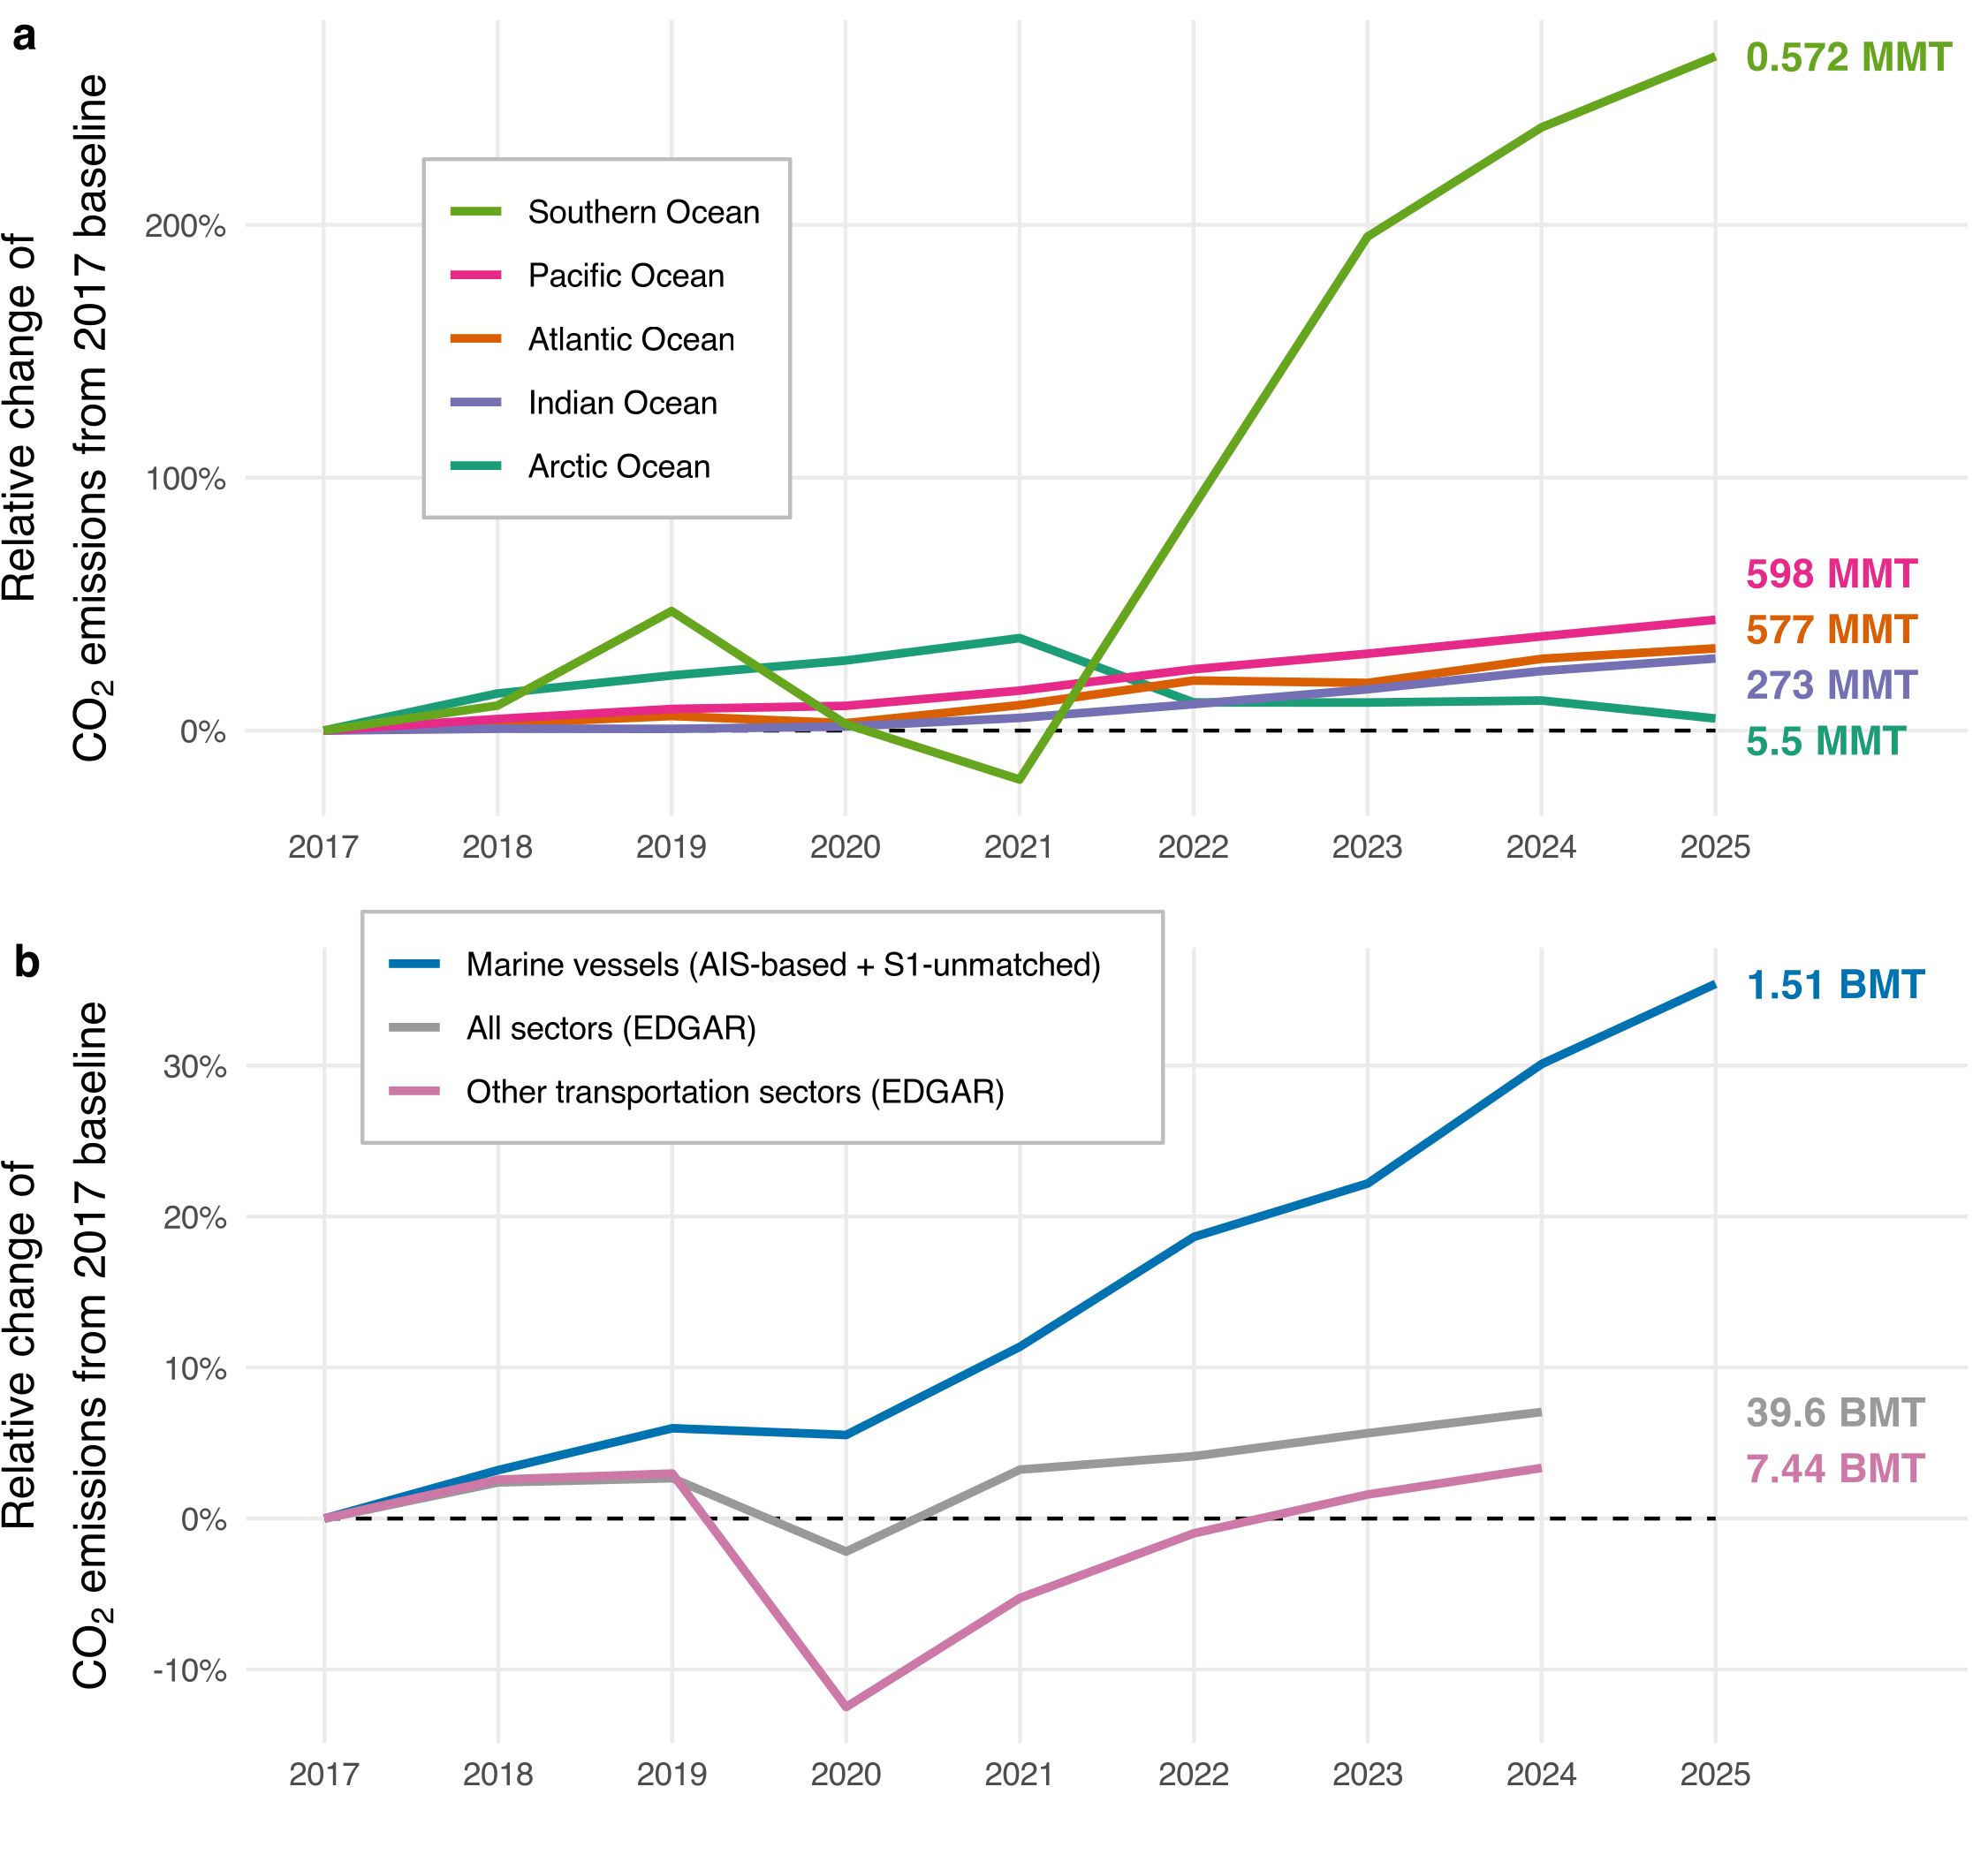
\includegraphics[width=\columnwidth]{figures/fig-emissions-marine-ocean-other-1.png}
%DIFDELCMD <     %%%
\DIFdelendFL \DIFaddbeginFL 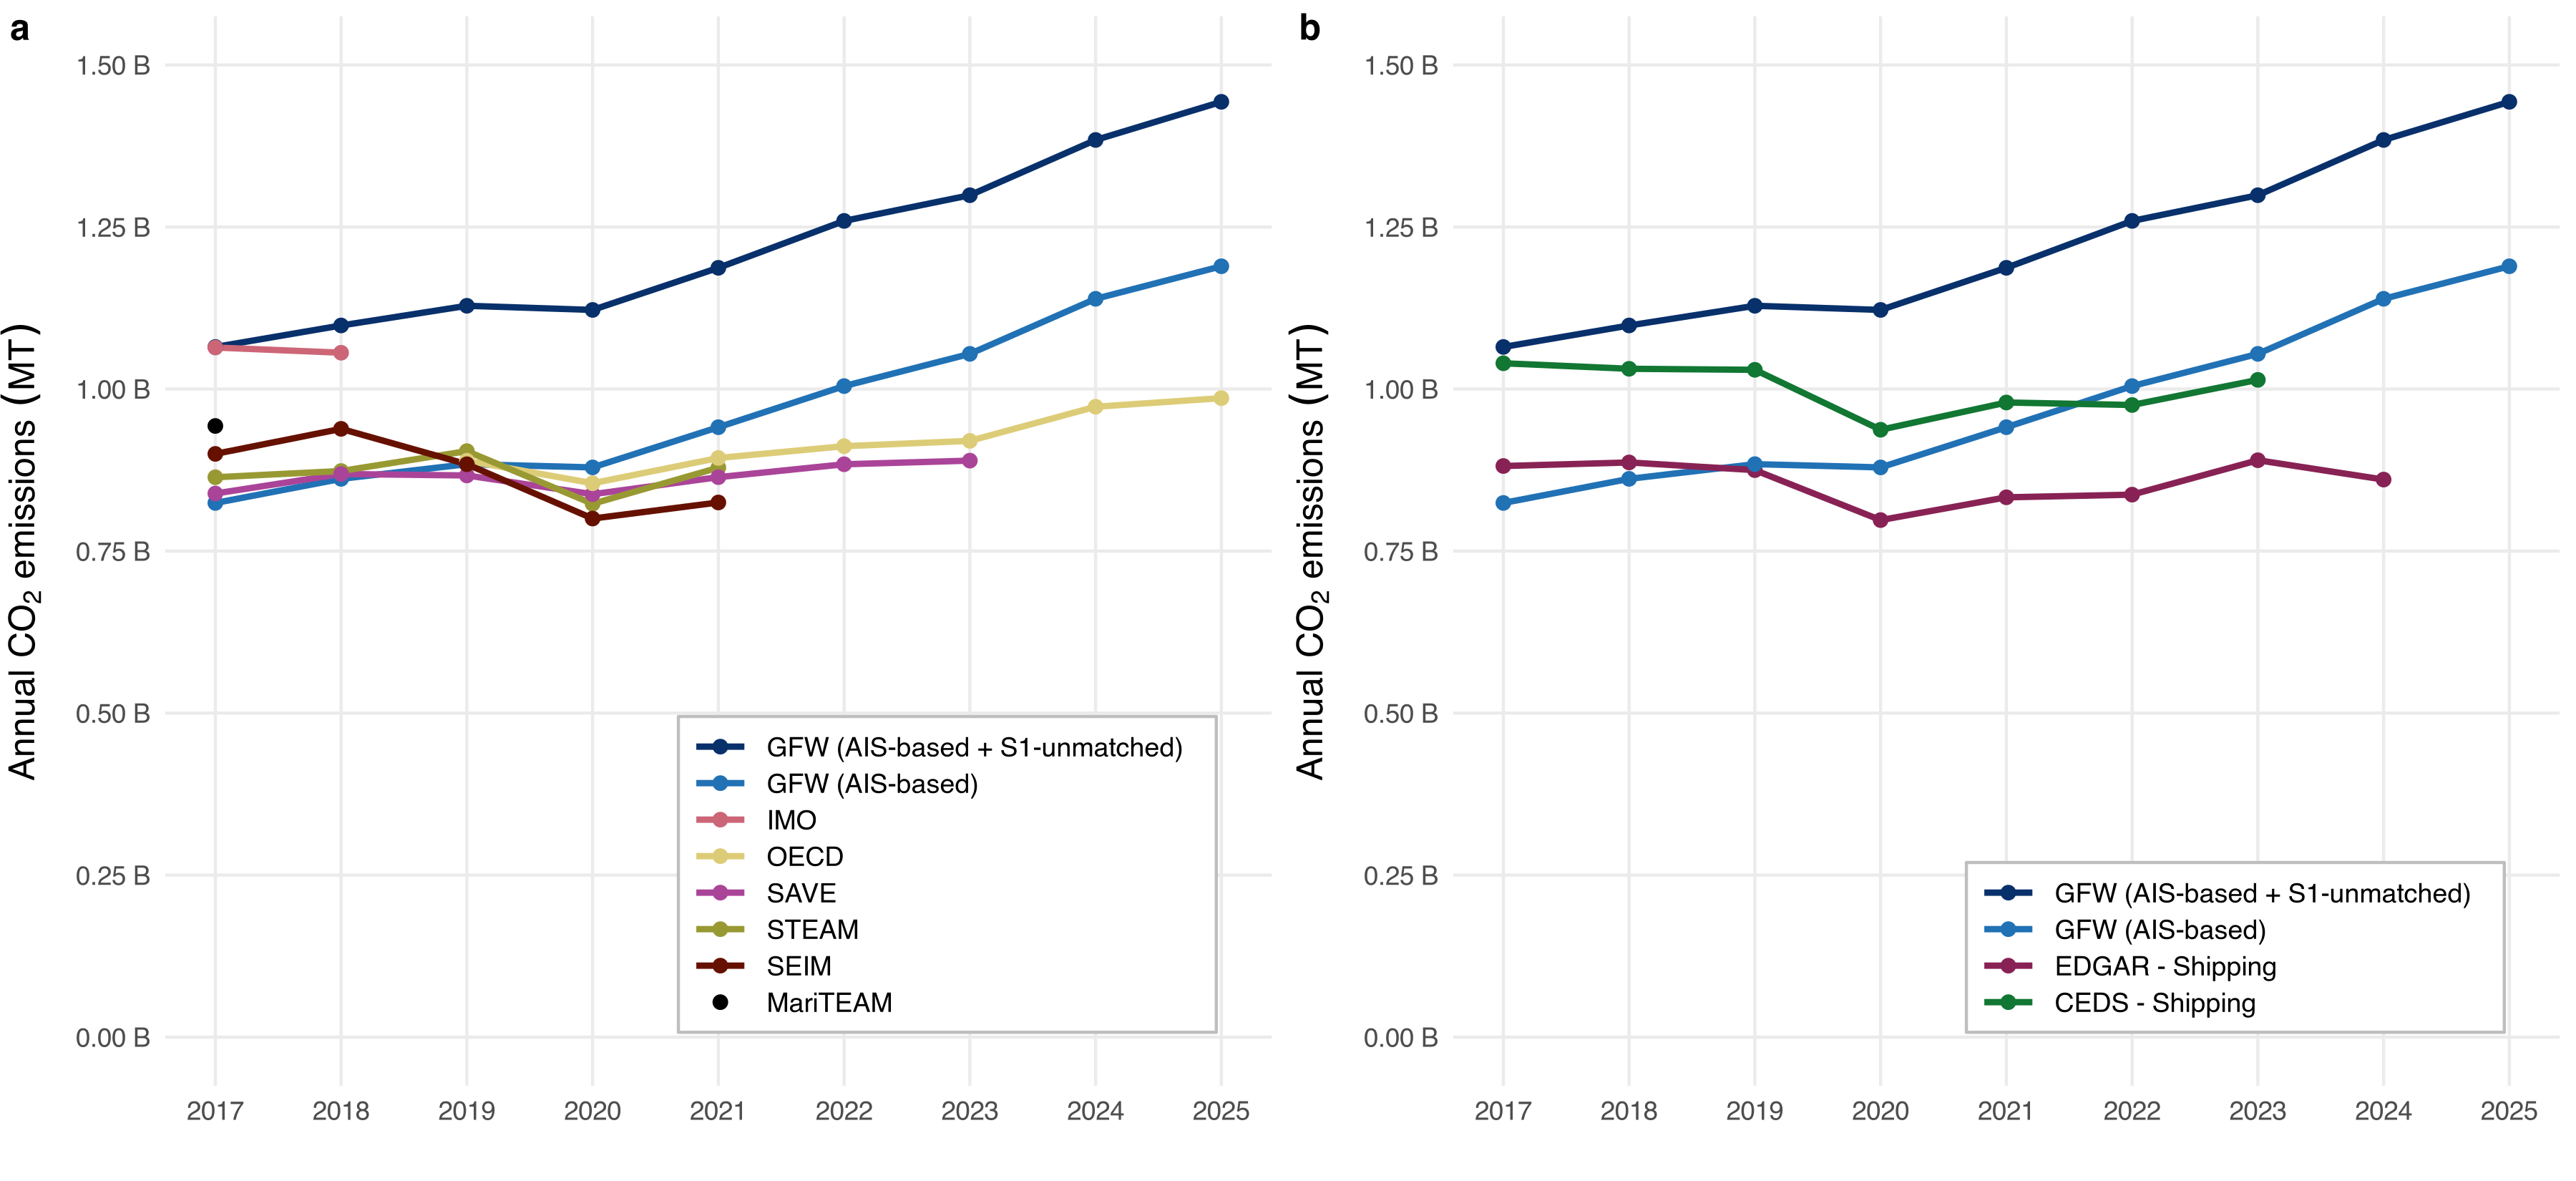
\includegraphics[width=\columnwidth]{figures/fig-emissions-inventory-comparison-1.png}
    \DIFaddendFL \caption{ (\DIFdelbeginFL \DIFdelFL{A}\DIFdelendFL \DIFaddbeginFL \DIFaddFL{a}\DIFaddendFL ) \DIFdelbeginFL \DIFdelFL{Trend in }\DIFdelendFL \DIFaddbeginFL \DIFaddFL{Annual }\DIFaddendFL CO$_{2}$ emissions \DIFdelbeginFL \DIFdelFL{by ocean (normalized to 2017 baseline), use }\DIFdelendFL \DIFaddbeginFL \DIFaddFL{from }\DIFaddendFL our \DIFaddbeginFL \DIFaddFL{AIS-based and }\DIFaddendFL fused \DIFdelbeginFL \DIFdelFL{AIS}\DIFdelendFL \DIFaddbeginFL \DIFaddFL{(AIS-based }\DIFaddendFL + \DIFdelbeginFL \DIFdelFL{S1 }\DIFdelendFL \DIFaddbeginFL \DIFaddFL{S1-unmatched) estimates against the other major bottom-up, AIS-based }\DIFaddendFL marine vessel \DIFdelbeginFL \DIFdelFL{data. (B) Comparison in trend of CO$_{2}$ }\DIFdelendFL emissions \DIFdelbeginFL \DIFdelFL{data }\DIFdelendFL \DIFaddbeginFL \DIFaddFL{inventories }\DIFaddendFL (\DIFdelbeginFL \DIFdelFL{normalized to 2017 baseline) between marine transportation emissions from GFW}\DIFdelendFL \DIFaddbeginFL \DIFaddFL{STEAM}\DIFaddendFL , \DIFdelbeginFL \DIFdelFL{other transportation emissions from EDGAR}\DIFdelendFL \DIFaddbeginFL \DIFaddFL{SEIM}\DIFaddendFL , \DIFaddbeginFL \DIFaddFL{MariTEAM, OECD, SAVE, }\DIFaddendFL and \DIFdelbeginFL \DIFdelFL{all sector emissions from EDGAR. On }\DIFdelendFL the \DIFdelbeginFL \DIFdelFL{right-hand side of the figure, 2024 absolute values }\DIFdelendFL \DIFaddbeginFL \DIFaddFL{Fourth IMO GHG Study). }\DIFaddendFL (\DIFdelbeginFL \DIFdelFL{in millions of metric tonnes}\DIFdelendFL \DIFaddbeginFL \DIFaddFL{b}\DIFaddendFL ) \DIFdelbeginFL \DIFdelFL{are shown as text }\DIFdelendFL \DIFaddbeginFL \DIFaddFL{The same two series against the top-down EDGAR }\DIFaddendFL and \DIFdelbeginFL \DIFdelFL{color-coded for each line}\DIFdelendFL \DIFaddbeginFL \DIFaddFL{CEDS shipping emissions inventories, which are derived from fuel statistics rather than from individual vessel activity}\DIFaddendFL .}
    \DIFdelbeginFL %DIFDELCMD < \label{fig:fig-emissions-marine-ocean-other}
%DIFDELCMD < %%%
\DIFdelendFL \DIFaddbeginFL \label{fig:fig-emissions-inventory-comparison}
\DIFaddendFL \end{figure}

\section{Discussion}

\DIFdelbegin \DIFdel{A high resolution understanding of marine vessel emissions is }\DIFdelend \DIFaddbegin \DIFadd{High-resolution emissions data for marine vessels are }\DIFaddend essential for designing\DIFdelbegin \DIFdel{effective policy solutions}\DIFdelend \DIFaddbegin \DIFadd{, implementing, and evaluating policies aimed at reducing them}\DIFaddend . However, incomplete vessel tracking data and technical data processing challenges have previously hindered progress \cite{chen2024analysis}. Our \DIFdelbegin \DIFdel{method, which overcomes these challenges , provides the necessary }\DIFdelend \DIFaddbegin \DIFadd{new data and methodology overcome these challenges by providing the }\DIFaddend spatiotemporal data necessary for analyzing interventions that could mitigate the GHG emissions that drive climate change, as well as other air pollutants that impact ambient air quality and health. \DIFdelbegin \DIFdel{One of the most promising such interventions would be the International Maritime Organization (IMO) Net-Zero Framework, which would establish the world's first global carbon market for marine vessel emissions with the goal of achieving net-zero GHG emissions from international shipping by 2050 \mbox{%DIFAUXCMD
\cite{IMO_MEPC83_2025}}\hskip0pt%DIFAUXCMD
. Additional types of interventions  include improved port queuing systems (e.g., in Los Angeles and Long Beach \mbox{%DIFAUXCMD
\cite{rhodes2025investigation}}\hskip0pt%DIFAUXCMD
), fuel standards  (e.g., sulfur and nitrogen control areas \mbox{%DIFAUXCMD
\cite{jutterstrom2021impact}}\hskip0pt%DIFAUXCMD
), other carbon markets (e.g., the EU Emissions Trading System \mbox{%DIFAUXCMD
\cite{mao2024towards}}\hskip0pt%DIFAUXCMD
), and vessel speed reduction zones (e.g., in California \mbox{%DIFAUXCMD
\cite{zobell2021underwater}}\hskip0pt%DIFAUXCMD
). }\DIFdelend Our data could also be used to quantify the spatial health impacts of air pollution related to shipping and fishing activity \cite{zhang2021global}, along with the associated environmental justice implications.

\DIFdelbegin \DIFdel{Carbon markets could play a role in mitigating marine vessel emissions, and accurate and high-resolution emissions data is critical for designing, monitoring, and evaluating such markets. The IMO is considering a global price on carbon }\DIFdelend \DIFaddbegin \DIFadd{There are three main implications of the results: First, the spatial and temporal detail of our dataset makes it directly relevant for climate change and air quality policy. Carbon pricing, fuel standards, emissions control areas, port queuing reforms, and vessel speed reduction programs all require credible baselines and measurable outcomes. Our estimates provide such a baseline for both broadcasting and non-broadcasting activity, including vessels that would be missed by AIS-only inventories. This is especially relevant for the IMO's effort to move international shipping toward net-zero greenhouse gas emissions by 2050 by implementing a carbon market }\DIFaddend for international shipping emissions by \DIFdelbegin \DIFdel{large vessels (}\DIFdelend \DIFaddbegin \DIFadd{vessels }\DIFaddend over 5,000 gross tonnage \DIFdelbegin \DIFdel{) \mbox{%DIFAUXCMD
\cite{imo_carbon_price}}\hskip0pt%DIFAUXCMD
, which will be discussed again for potential adoption in October, 2026 \mbox{%DIFAUXCMD
\cite{IMO2025NetZero}}\hskip0pt%DIFAUXCMD
. In recent years}\DIFdelend \DIFaddbegin \DIFadd{\mbox{%DIFAUXCMD
\cite{imo_carbon_price, IMO2025NetZero, kang2026maritime}}\hskip0pt%DIFAUXCMD
. Further}\DIFaddend , the European Union Emissions Trading System has \DIFdelbegin \DIFdel{already }\DIFdelend been expanded to include marine transportation under the EU emissions cap, and to subject vessel activity to and from European Economic Area ports to a carbon price \cite{kotzampasakis2025maritime}. Implementing a carbon market based on limiting emissions intensity (the amount of emissions per unit of activity or production) could \DIFaddbegin \DIFadd{also }\DIFaddend be an effective strategy for mitigating marine vessel emissions, even with a growing number of vessels. Carbon markets \DIFdelbegin \DIFdel{that are based on carbon credits for emissions intensity rather than just on capping emissions }\DIFdelend \DIFaddbegin \DIFadd{based on emissions-intensity standards rather than absolute emissions caps}\DIFaddend , such as India's emerging carbon market \cite{gupta2023assessing}, allow \DIFdelbegin \DIFdel{for overall }\DIFdelend economic growth while \DIFdelbegin \DIFdel{still incentivizing more efficient activity. This }\DIFdelend \DIFaddbegin \DIFadd{continuing to incentivize improvements in emissions efficiency. This policy design }\DIFaddend is consistent with a review paper on current marine vessel emissions datasets, which concluded that measures aimed at increasing technical efficiency of ships could be an effective way to decouple emissions growth from global trade demand \cite{dengreview}.

\DIFdelbegin \DIFdel{With a more complete picture of global emissions at sea, we are in a position to understand the magnitude of the }\DIFdelend \DIFaddbegin \DIFadd{Second, our data can be used to calculate the }\DIFaddend climate externality social cost \DIFdelbegin \DIFdel{(SC) }\DIFdelend associated with marine \DIFdelbegin \DIFdel{vessels, and how it compares to the }\DIFdelend \DIFaddbegin \DIFadd{vessel activity, which can be compared against the economic }\DIFaddend value of the \DIFdelbegin \DIFdel{products these vessels carry? First we look at }\DIFdelend \DIFaddbegin \DIFadd{activities; we conduct a simple version of that calculation here. We first focus on }\DIFaddend non-fishing vessels (e.g., cargo \DIFdelbegin \DIFdel{, tanker, etc.}\DIFdelend \DIFaddbegin \DIFadd{ships and tankers}\DIFaddend ) and compare \DIFdelbegin \DIFdel{the SC to the total }\DIFdelend \DIFaddbegin \DIFadd{their climate externalities with the }\DIFaddend value of goods \DIFdelbegin \DIFdel{traded at sea. By multiplying the social cost }\DIFdelend \DIFaddbegin \DIFadd{transported by sea. Multiplying our estimated emissions of carbon dioxide, methane, and nitrous oxide from non-fishing vessels by the corresponding social costs }\DIFaddend of carbon (283 USD/MT \cite{moore2024synthesis}), \DIFdelbegin \DIFdel{social cost of }\DIFdelend methane (2,900 USD/MT \cite{wang2023damage}), and \DIFdelbegin \DIFdel{social cost of }\DIFdelend nitrous oxide (49,600 USD/MT \cite{wang2023damage}) \DIFdelbegin \DIFdel{each respectively with our estimated emissions for these GHGs from non-fishing vessels, we estimate an }\DIFdelend \DIFaddbegin \DIFadd{yields an estimated }\DIFaddend annual global climate externality of \DIFdelbegin \DIFdel{318 billion USD for non-fishing vessels }\DIFdelend \DIFaddbegin \DIFadd{322 billion USD }\DIFaddend in 2021 (\DIFaddbegin \DIFadd{Supplementary }\DIFaddend Table \ref{tab:social_cost_summary_tbl}). This \DIFdelbegin \DIFdel{represents }\DIFdelend \DIFaddbegin \DIFadd{amounts to }\DIFaddend about 5\% of the total value of \DIFdelbegin \DIFdel{all }\DIFdelend goods transported by maritime trade\DIFdelbegin \DIFdel{(using }\DIFdelend \DIFaddbegin \DIFadd{, based on an estimated }\DIFaddend 6.63 trillion USD \DIFdelbegin \DIFdel{as the }\DIFdelend \DIFaddbegin \DIFadd{in global seaborne trade in }\DIFaddend 2021 \DIFdelbegin \DIFdel{value of maritime-traded goods \mbox{%DIFAUXCMD
\cite{hoffmeister2022developing}}\hskip0pt%DIFAUXCMD
). By doing the same }\DIFdelend \DIFaddbegin \DIFadd{\mbox{%DIFAUXCMD
\cite{hoffmeister2022developing}}\hskip0pt%DIFAUXCMD
. Repeating this }\DIFaddend calculation for fishing vessels \DIFdelbegin \DIFdel{, we estimate an }\DIFdelend \DIFaddbegin \DIFadd{yields an estimated }\DIFaddend annual global climate externality of \DIFdelbegin \DIFdel{22 billion USD for fishing vessels }\DIFdelend \DIFaddbegin \DIFadd{23 billion USD }\DIFaddend in 2022 (\DIFaddbegin \DIFadd{Supplementary }\DIFaddend Table \ref{tab:social_cost_summary_tbl}). This \DIFdelbegin \DIFdel{represents about 14}\DIFdelend \DIFaddbegin \DIFadd{amounts to about 15}\DIFaddend \% of the \DIFdelbegin \DIFdel{total value of global capture fisheries(using }\DIFdelend \DIFaddbegin \DIFadd{global first-sale value of capture fisheries, which totaled }\DIFaddend 159 billion USD \DIFdelbegin \DIFdel{as the }\DIFdelend \DIFaddbegin \DIFadd{in }\DIFaddend 2022 \DIFdelbegin \DIFdel{total first sale value \mbox{%DIFAUXCMD
\cite{fisheries2024state}}\hskip0pt%DIFAUXCMD
). Using a similar approach, our }\DIFdelend \DIFaddbegin \DIFadd{\mbox{%DIFAUXCMD
\cite{fisheries2024state}}\hskip0pt%DIFAUXCMD
. Our }\DIFaddend voyage-level emissions dataset \DIFdelbegin \DIFdel{could }\DIFdelend \DIFaddbegin \DIFadd{can }\DIFaddend be used to estimate the \DIFdelbegin \DIFdel{social cost climate externalities for }\DIFdelend \DIFaddbegin \DIFadd{climate externalities associated with }\DIFaddend country-to-country trade flows, \DIFdelbegin \DIFdel{allowing for the calculation of country-to-country }\DIFdelend \DIFaddbegin \DIFadd{enabling the construction of }\DIFaddend metrics such as the \DIFdelbegin \DIFdel{SC per USD value of goods traded , or the SC }\DIFdelend \DIFaddbegin \DIFadd{social cost per dollar of traded goods or the social cost }\DIFaddend per metric tonne of \DIFdelbegin \DIFdel{goods traded}\DIFdelend \DIFaddbegin \DIFadd{cargo transported}\DIFaddend . For vessels tracked with AIS, \DIFdelbegin \DIFdel{it is also possible to assign an externality cost to }\DIFdelend \DIFaddbegin \DIFadd{these externality costs can also be assigned to }\DIFaddend individual port-to-port \DIFdelbegin \DIFdel{trips. In addition to climate externalities, marine transportation contributes to significant human health impacts arising from air pollution }\DIFdelend \DIFaddbegin \DIFadd{voyages. Beyond their contribution to climate change, marine vessels emit air pollutants that impose substantial human health costs that have yet to be fully understood }\DIFaddend \cite{zhang2021global}.

\DIFdelbegin \DIFdel{Our approach provides an example of how to resolve a more general }\DIFdelend \DIFaddbegin \DIFadd{Third, our methodology and data can help address a broader }\DIFaddend challenge in environmental monitoring: \DIFdelbegin \DIFdel{the temporal trend in an environmental variable is }\DIFdelend \DIFaddbegin \DIFadd{temporal trends in environmental variables are }\DIFaddend often confounded by changes in monitoring \DIFdelbegin \DIFdel{itself}\DIFdelend \DIFaddbegin \DIFadd{effort}\DIFaddend . For marine vessel emissions, this challenge \DIFdelbegin \DIFdel{manifests as an increase in }\DIFdelend \DIFaddbegin \DIFadd{arises because the }\DIFaddend adoption of AIS and \DIFaddbegin \DIFadd{the }\DIFaddend number of vessels being tracked \DIFaddbegin \DIFadd{have increased }\DIFaddend over time, \DIFdelbegin \DIFdel{which lead current methods }\DIFdelend \DIFaddbegin \DIFadd{causing AIS-only estimates }\DIFaddend to overestimate the \DIFdelbegin \DIFdel{rate of }\DIFdelend \DIFaddbegin \DIFadd{2017--2025 }\DIFaddend growth of at-sea emissions \DIFdelbegin \DIFdel{(by 15.9\% ). Similarly, more extensive monitoring of }\DIFdelend \DIFaddbegin \DIFadd{by 8.8 percentage points (44\% rather than 36\%). Similar biases may arise for }\DIFaddend other environmental variables \DIFdelbegin \DIFdel{could lead us to overestimate their growth rates (for example, for invasive species discoveries \mbox{%DIFAUXCMD
\cite{costello2003pattern}}\hskip0pt%DIFAUXCMD
). Our approach that fuses }\DIFdelend \DIFaddbegin \DIFadd{when monitoring expands over time, such as the discovery of invasive species \mbox{%DIFAUXCMD
\cite{costello2003pattern}}\hskip0pt%DIFAUXCMD
. By combining }\DIFaddend two independent data sources\DIFaddbegin \DIFadd{, our approach }\DIFaddend is more robust to changes in monitoring \DIFdelbegin \DIFdel{over time than methods relying }\DIFdelend \DIFaddbegin \DIFadd{effort than methods that rely }\DIFaddend on a single \DIFdelbegin \DIFdel{data source, and }\DIFdelend \DIFaddbegin \DIFadd{source. The same framework }\DIFaddend could be applied in other settings \DIFdelbegin \DIFdel{to produce unbiased estimates of environmental change}\DIFdelend \DIFaddbegin \DIFadd{where changes in monitoring complicate the measurement of long-run environmental trends}\DIFaddend .

\DIFdelbegin \DIFdel{Several caveats remain. Our }\DIFdelend \DIFaddbegin \DIFadd{Our approach is complementary to, rather than a replacement for, efforts to improve AIS data quality. Any AIS-derived inventory faces two distinct gaps: 1) vessels that do not use AIS; and 2) vessels that use AIS, but whose signals are not received due to gaps in AIS transmissions or reception. Trajectory reconstruction addresses the second but cannot address the first. Reconstruction also cannot resolve the confound between monitoring and activity: because reconstruction methods are calibrated on observed AIS, discrete shifts in coverage — such as the 2022 adoption of D-AIS or the 2021 loss of terrestrial reception in Chinese waters (Supplementary Note \ref{sec:ais-receiver-types}) — propagate into reconstructed trajectories. S1 observation effort is independent of AIS coverage, which makes our estimates of the emissions trend less sensitive to such shifts than estimates based on AIS alone. The value of our framework is therefore that it tolerates incomplete AIS: unmatched detections absorb emissions from both }\DIFaddend non-broadcasting \DIFdelbegin \DIFdel{emissions model hinges on one key assumption: }\DIFdelend \DIFaddbegin \DIFadd{vessels and broadcasting vessels whose activity is missing from the AIS record, so comprehensive emissions can be recovered without first achieving a `perfect' AIS reconstruction. Our own AIS-based component nonetheless rests on a single AIS data pipeline, GFW's. AIS records assembled by other providers and pipelines differ in coverage and cleaning, so AIS-based totals and trends derived from them would differ from ours, although activity missing from any one AIS record can still be captured through unmatched S1 detections.
}

\DIFadd{Several methodological limitations remain. One key assumption is that S1-unmatched emissions can be inferred from }\DIFaddend the \DIFdelbegin \DIFdel{relationship between unmatched vessel detections and non-broadcasting emissions is similar to the }\DIFdelend relationship between \DIFdelbegin \DIFdel{matched vessel detections and AIS-broadcasting emissions }\DIFdelend \DIFaddbegin \DIFadd{S1 detections and AIS-based emissions for matched vessels}\DIFaddend . We believe this is a reasonable assumption for several reasons. \DIFdelbegin \DIFdel{Perhaps the strongest reason is that many unmatched detections from }\DIFdelend \DIFaddbegin \DIFadd{First, some unmatched }\DIFaddend S1 \DIFdelbegin \DIFdel{inevitably are actually just }\DIFdelend \DIFaddbegin \DIFadd{detections correspond to }\DIFaddend AIS-broadcasting vessels that are \DIFdelbegin \DIFdel{either experiencing gaps in transmission, or are broadcasting in areas with poor AIS reception quality. }\DIFdelend \DIFaddbegin \DIFadd{not observed in the AIS data because of transmission gaps or poor reception quality; we estimate that about 6.2\% of unmatched detections are broadcasting vessels missed during AIS gaps alone (Fig. \ref{fig:fig-s1-matching-double-counting}). }\DIFaddend In these cases, the relationship between S1 vessel detections and emissions \DIFdelbegin \DIFdel{would hold perfectly }\DIFdelend \DIFaddbegin \DIFadd{should hold closely, }\DIFaddend since these unmatched vessels are \DIFdelbegin \DIFdel{in fact just }\DIFdelend AIS-broadcasting vessels that happen \DIFdelbegin \DIFdel{to not }\DIFdelend \DIFaddbegin \DIFadd{not to }\DIFaddend be observed by AIS at a given point in time. Second, our model accounts for vessel length, a proxy for main engine power \DIFdelbegin \DIFdel{which }\DIFdelend \DIFaddbegin \DIFadd{that }\DIFaddend is one of the \DIFdelbegin \DIFdel{most important components of AIS-based emissions modeling that can be used for any vessel that uses an internal combustion engine}\DIFdelend \DIFaddbegin \DIFadd{primary determinants of emissions in AIS-based models and is applicable to virtually all vessels powered by internal combustion engines}\DIFaddend . Third, since fishing and non-fishing vessels are known to have different emissions factors \cite{coello2015ais}, we account for this by differentiating detections between fishing and non-fishing vessels. Finally, \DIFdelbegin \DIFdel{by including spatiotemporal features in our model , }\DIFdelend \DIFaddbegin \DIFadd{our model incorporates spatiotemporal features that allow }\DIFaddend the relationship between detections and emissions \DIFdelbegin \DIFdel{can }\DIFdelend \DIFaddbegin \DIFadd{to }\DIFaddend vary across space and time. \DIFdelbegin \DIFdel{This means that if the types of broadcasting }\DIFdelend \DIFaddbegin \DIFadd{Consequently, if AIS-broadcasting }\DIFaddend and non-broadcasting vessels operating in a given place and time \DIFdelbegin \DIFdel{are similar }\DIFdelend \DIFaddbegin \DIFadd{have similar characteristics}\DIFaddend , the relationship between detections and emissions \DIFdelbegin \DIFdel{should be similar there }\DIFdelend \DIFaddbegin \DIFadd{is expected to be similar }\DIFaddend as well. \DIFdelbegin \DIFdel{Nonetheless, the relationship may not always }\DIFdelend \DIFaddbegin \DIFadd{S1 detections also exclude vessels within 1 km of shore and at known anchorages. This does not by itself bias our S1-unmatched estimates downward, because the emissions regression is trained on AIS-based emissions that include activity in those areas: our model learns how much total emissions accompany the detections S1 can observe, and applies the same relationship to unmatched detections. This assumes that non-broadcasting vessels divide their activity between observed and unobserved waters in the same way as broadcasting vessels of the same type in similar locations; our S1-unmatched estimates would be too low if non-broadcasting vessels are more concentrated in coastal waters and ports, and too high if they spend less time in coastal waters and ports.
}

\DIFadd{The relationship between detections and emissions may fail to }\DIFaddend hold for non-broadcasting vessels \DIFdelbegin \DIFdel{, particularly if these vessels have vastly different emissions factors than the ones we use }\DIFdelend \DIFaddbegin \DIFadd{if their emissions factors differ substantially }\DIFaddend from the IMO \DIFdelbegin \DIFdel{for converting energy use to emissions \mbox{%DIFAUXCMD
\cite{fourth2020greenhouse} }\hskip0pt%DIFAUXCMD
(}\DIFdelend \DIFaddbegin \DIFadd{values we use to convert energy use into emissions \mbox{%DIFAUXCMD
\cite{fourth2020greenhouse}}\hskip0pt%DIFAUXCMD
. This could arise, }\DIFaddend for example, \DIFdelbegin \DIFdel{vessels using newer engine and fuel types }\DIFdelend \DIFaddbegin \DIFadd{if non-broadcasting vessels disproportionately use newer and more efficient engine or fuel technologies }\DIFaddend that were not \DIFdelbegin \DIFdel{as common }\DIFdelend \DIFaddbegin \DIFadd{widely represented }\DIFaddend when the IMO \DIFdelbegin \DIFdel{report was written }\DIFdelend \DIFaddbegin \DIFadd{emissions factors were developed }\DIFaddend in 2020\DIFdelbegin \DIFdel{). This brings us to }\DIFdelend \DIFaddbegin \DIFadd{; this would have the impact of biasing our S1-unmatched emissions estimates too high. Conversely, if non-broadcasting vessels instead use severely outdated and inefficient engine technologies, this would have the impact of biasing our S1-unmatched emissions estimates too low. Because S1-unmatched emissions make up 18\% of our 2025 fused emissions total, a proportional bias of this kind would change our total fused emissions by only 18\% as much: a 20\% bias in either direction would change our 2025 total by about 3.5\%, and our 2017--2025 growth by at most 1.4 percentage points (to between 34\% and 37\%, against our estimate of 36\%). Emissions factors are also }\DIFaddend one of the primary limitations of the \DIFdelbegin \DIFdel{AIS model . Since the specific engine type and fuel used for each vessel is not usually publicly known, we used }\DIFdelend \DIFaddbegin \DIFadd{AIS-based model our methodology builds upon. Since information on the fuel type used by individual vessels is generally not publicly available, we rely on }\DIFaddend weighted average emissions factors from the IMO \cite{fourth2020greenhouse}. \DIFdelbegin \DIFdel{In reality, different engine types and fuel types have different emissions factors, meaning that vessels using engines and fuel types that are significantly different than }\DIFdelend \DIFaddbegin \DIFadd{Vessel-level emissions estimates based on average emission factors may be biased if a particular vessel's engine or fuel type is not well represented in }\DIFaddend the global fleet\DIFdelbegin \DIFdel{may have biased vessel-level emissions estimates}\DIFdelend . This could be an important consideration \DIFdelbegin \DIFdel{if }\DIFdelend \DIFaddbegin \DIFadd{when }\DIFaddend using the model to explore policies aimed at technological engine changes and fuel switching. \DIFdelbegin \DIFdel{If and }\DIFdelend \DIFaddbegin \DIFadd{However, }\DIFaddend when this type of vessel-level information becomes publicly available, our modeling framework could easily be adapted to incorporate it. Despite the fact that we do not currently explicitly account for vessel-level \DIFdelbegin \DIFdel{engine and }\DIFdelend fuel type, our vessel-level emissions model still achieves high performance when validated against two fully independent vessel-level datasets \DIFdelbegin \DIFdel{. Finally, neither AISnor Sentinel-1 have }\DIFdelend \DIFaddbegin \DIFadd{(Figs. \ref{fig:fig-registered-data-performance}--\ref{fig:fig-mrv-performance}). 
}

\DIFadd{The difference between our AIS-based emissions and other bottom-up inventories is primarily one of fleet scope rather than of the emissions modeling itself (Supplementary Note \ref{sec:methods-comparison}). Global AIS-based emissions are likely understated whenever heavy reliance on registry-defined fleets leaves low-information vessels out of scope. The vessels in our analysis are not limited to only those that are registered, but rather include all vessels that carry AIS; the fleet thus expands with increasing uptake of AIS among vessels, with the largest share of our estimated emissions growth carried by small vessels that registries cover least. This indicates that the other bottom-up inventories, and our own estimates for early years, likely miss part of the global fleet (Supplementary Note \ref{sec:inventory-comparison}). Our data fusion approach extends on this even further, expanding our estimates to include large vessels that appear in neither registries nor AIS, which also contributes to the magnitude gap with the top-down EDGAR and CEDS inventories. 
}

\DIFadd{Our estimated growth rate is higher than those of other inventories, which warrants closer inspection. For our AIS-based results, 50\% of the 2017--2025 increase comes from vessels under 50 m, led by small passenger vessels (35\% of the increase) and small fishing vessels (10\%), segments that our inventory captures more fully than other inventories and that have grown fastest in both number of vessels and emissions (Supplementary Table \ref{tab:growth_share_by_family_length}; Supplementary Figs. \ref{fig:figS-fleet-growth-by-year}--\ref{fig:figS-fleet-sankey-with-series-2025}). Most of the rest (40\%) comes from vessels of 150 m and over, nearly all of them cargo vessels and tankers. This AIS-based growth combines three effects: increased activity, improved AIS reception (e.g., from D-AIS), and wider use of AIS among these vessels. Splitting each segment's change into its number of vessels, the distance each vessel travels, and the emissions per nautical mile shows that nearly all of the growth from small passenger vessels comes from more vessels appearing in AIS, whereas much of the growth from small fishing vessels comes from the same vessels being tracked over more distance, as improved reception fills gaps in their tracks (Supplementary Table \ref{tab:growth_decomposition_by_family_length}). Our data fusion approach lets us partly disentangle these effects. Looking at our S1 detection data, we see that the fraction of vessel detections matched to AIS is generally increasing over time, particularly for small vessels (Supplementary Fig. \ref{fig:figS-ais-carriage-saturation-by-size}). Part of the AIS-based growth therefore reflects wider AIS use; within our data fusion framework, these vessels' emissions are simply transferred from our S1-unmatched component to our AIS-based component as soon as they begin carrying AIS. However, even increasing adoption of AIS does not fully explain the scale of increasing emissions: although unmatched detections of small non-fishing vessels are going down slightly over time, consistent with vessels adopting AIS, matched detections are going up much more significantly. This translates into an overall increase in detected vessels, reflecting increased vessel activity in that segment (Supplementary Fig. \ref{fig:figS-density-by-match-status}, panel a). This provides new evidence supporting the concept of the `blue acceleration' and the expansion of human activity in the oceans \mbox{%DIFAUXCMD
\cite{jouffray2020blue}}\hskip0pt%DIFAUXCMD
. Even with data fusion, our approach is limited by the observational capacity of both AIS and S1. Neither AIS nor S1 has }\DIFaddend good coverage for very small vessels (i.e., $<$15m), \DIFdelbegin \DIFdel{limiting our approach to only represent emissions from large marine vessels. }\DIFdelend \DIFaddbegin \DIFadd{and S1 rarely detects wood and fiberglass vessels. Vessels that neither system observes are missing from our fused estimates, which are therefore likely an underestimate of true global marine vessel emissions. There also may be many small and coastal vessels that S1 could not detect in early years of our dataset, because of their size or hull material or because they operate only within the shoreline buffer, but which later adopted AIS. This could bias our increasing trend upward compared to the true trend in activity, even when looking at our fused estimates (Supplementary Note \ref{sec:inventory-comparison}). Further research could help disentangle the magnitude and trends of small and coastal vessels. }\DIFaddend An exciting area of future work would be to incorporate new satellite sensors into our data fusion framework to \DIFdelbegin \DIFdel{quantify emissions }\DIFdelend \DIFaddbegin \DIFadd{better capture activity }\DIFaddend from small vessels (e.g., optical imagery from Sentinel-2 or \DIFdelbegin \DIFdel{Planet}\DIFdelend \DIFaddbegin \DIFadd{PlanetScope \mbox{%DIFAUXCMD
\cite{wei2026satellite}}\hskip0pt%DIFAUXCMD
}\DIFaddend ).

\DIFdelbegin \DIFdel{Measuring }\DIFdelend %DIF >  Still, even confined to non-fishing vessels of 150m and above---the segment of the fleet where AIS use was already widespread at the start of our series , and thus where measured growth reflects activity at sea and AIS quality rather than expanding AIS use---our AIS-based emissions grew at a compound annual rate of 3.20\%, nearly twice that of the fastest-growing bottom-up inventories, more than three times that of global emissions across all sectors, and about six to seven times that of all other transportation modes combined (Supplementary Fig. \ref{fig:figS-inventory-comparison-all-sources}, Supplementary Table \ref{tab:inventory_growth_comparison}).
\DIFaddbegin 

\DIFadd{Accurately measuring }\DIFaddend emissions is a necessary step towards reducing them. \DIFdelbegin \DIFdel{Until now}\DIFdelend \DIFaddbegin \DIFadd{To date}\DIFaddend , quantifying emissions from vessels in the ocean has \DIFdelbegin \DIFdel{been a challenge due to }\DIFdelend \DIFaddbegin \DIFadd{suffered from }\DIFaddend incomplete monitoring at-sea and the opaque nature of vessel characteristics. \DIFdelbegin \DIFdel{By fusing }\DIFdelend \DIFaddbegin \DIFadd{We fuse }\DIFaddend two satellite-based data sources \DIFdelbegin \DIFdel{that combined }\DIFdelend \DIFaddbegin \DIFadd{and, by doing so, }\DIFaddend are able to track emissions from both broadcasting and non-broadcasting activity\DIFdelbegin \DIFdel{, and also }\DIFdelend \DIFaddbegin \DIFadd{. Furthermore, }\DIFaddend by estimating key emissions modeling vessel characteristics for hundreds of thousands of vessels, we now have a comprehensive and high resolution picture of emissions from large marine vessels. This can serve as the foundation for \DIFdelbegin \DIFdel{work }\DIFdelend \DIFaddbegin \DIFadd{interventions }\DIFaddend aimed at decarbonizing the marine sector and reducing the health impacts of marine air pollution.

%DIF < %%%%%%%%%%%%%%% REFERENCES %%%%%%%%%%%%%%%
\DIFaddbegin \section*{\DIFadd{Methods}}
\DIFaddend 

\DIFdelbegin %DIFDELCMD < \clearpage 
%DIFDELCMD < 

%DIFDELCMD < \bibliography{bibliography}
%DIFDELCMD < 

%DIFDELCMD < %%%
\section*{\DIFdel{Acknowledgments}}
%DIFAUXCMD
%DIFDELCMD < 

%DIFDELCMD < %%%
\paragraph*{\DIFdel{Funding:}} 
%DIFAUXCMD
%DIFDELCMD < 

%DIFDELCMD < %%%
\DIFdel{We gratefully thank Climate TRACE for supporting this research.
}%DIFDELCMD < 

%DIFDELCMD < %%%
\paragraph*{\DIFdel{Author contributions:}}
%DIFAUXCMD
%DIFDELCMD < 

%DIFDELCMD < %%%
\DIFdel{Conceptualization: GM and DK; Methodology: GM, PCM, OD, EFC, AH, DK,MP, ZW, and CC; Software:  GM, PCM, EFC, AH, and ZW Validation: GM, PCM, DK,MP; Formal analysis: GM, PCM, OD, EFC, AH, DK,MP, ZW, and CC; Investigation: GM, PCM, OD, EFC, AH, DK,MP, ZW, and CC; Data curation:  GM, PCM, EFC, AH, DK,MP and ZW ; Writing - Original Draft: GM, PCM, OD, and CC; Writing -Review \& Editing: GM, PCM, OD, JB, EFC, AH, DK, FSP, MP, ZW, and CC; Visualization: GM and PCM; Supervision: OD, and CC; Project administration: JB; Funding acquisition: GM, PCM, JB, DK, and CC
}%DIFDELCMD < 

%DIFDELCMD < %%%
\paragraph*{\DIFdel{Competing interests:}}
%DIFAUXCMD
%DIFDELCMD < 

%DIFDELCMD < %%%
\DIFdel{There are no competing interests to declare.
}%DIFDELCMD < 

%DIFDELCMD < %%%
\paragraph*{\DIFdel{Data and materials availability:}} %DIFAUXCMD
\DIFdel{All code and data necessary for reproducing this figures and tables in this analysis will be made available in a public GitHub repository with an accompanying Zenodo repository and DOI}\DIFdelend \DIFaddbegin \DIFadd{Our use of a large language model as a programming and editing assistant in preparing this work is described under `Use of generative AI' below}\DIFaddend .

\DIFdelbegin \section*{\DIFdel{Methods}}
%DIFAUXCMD
%DIFDELCMD < 

%DIFDELCMD < %%%
\DIFdelend This work relies on multiple sources of spatial and tabular data to assess marine vessel emissions globally. We use AIS data, vessel registry information \DIFdelbegin \DIFdel{, Sentinel-1 and Sentinel-2 }\DIFdelend \DIFaddbegin \DIFadd{and Sentinel-1 (S1) }\DIFaddend derived data to construct our AIS-based emission model and the \DIFdelbegin \DIFdel{non-broadcasting }\DIFdelend \DIFaddbegin \DIFadd{S1-unmatched }\DIFaddend emissions model (Fig. \ref{fig:gfw_emissions_framework_flowchart}).

\begin{figure}[H]
    \centering
    \DIFdelbeginFL %DIFDELCMD < 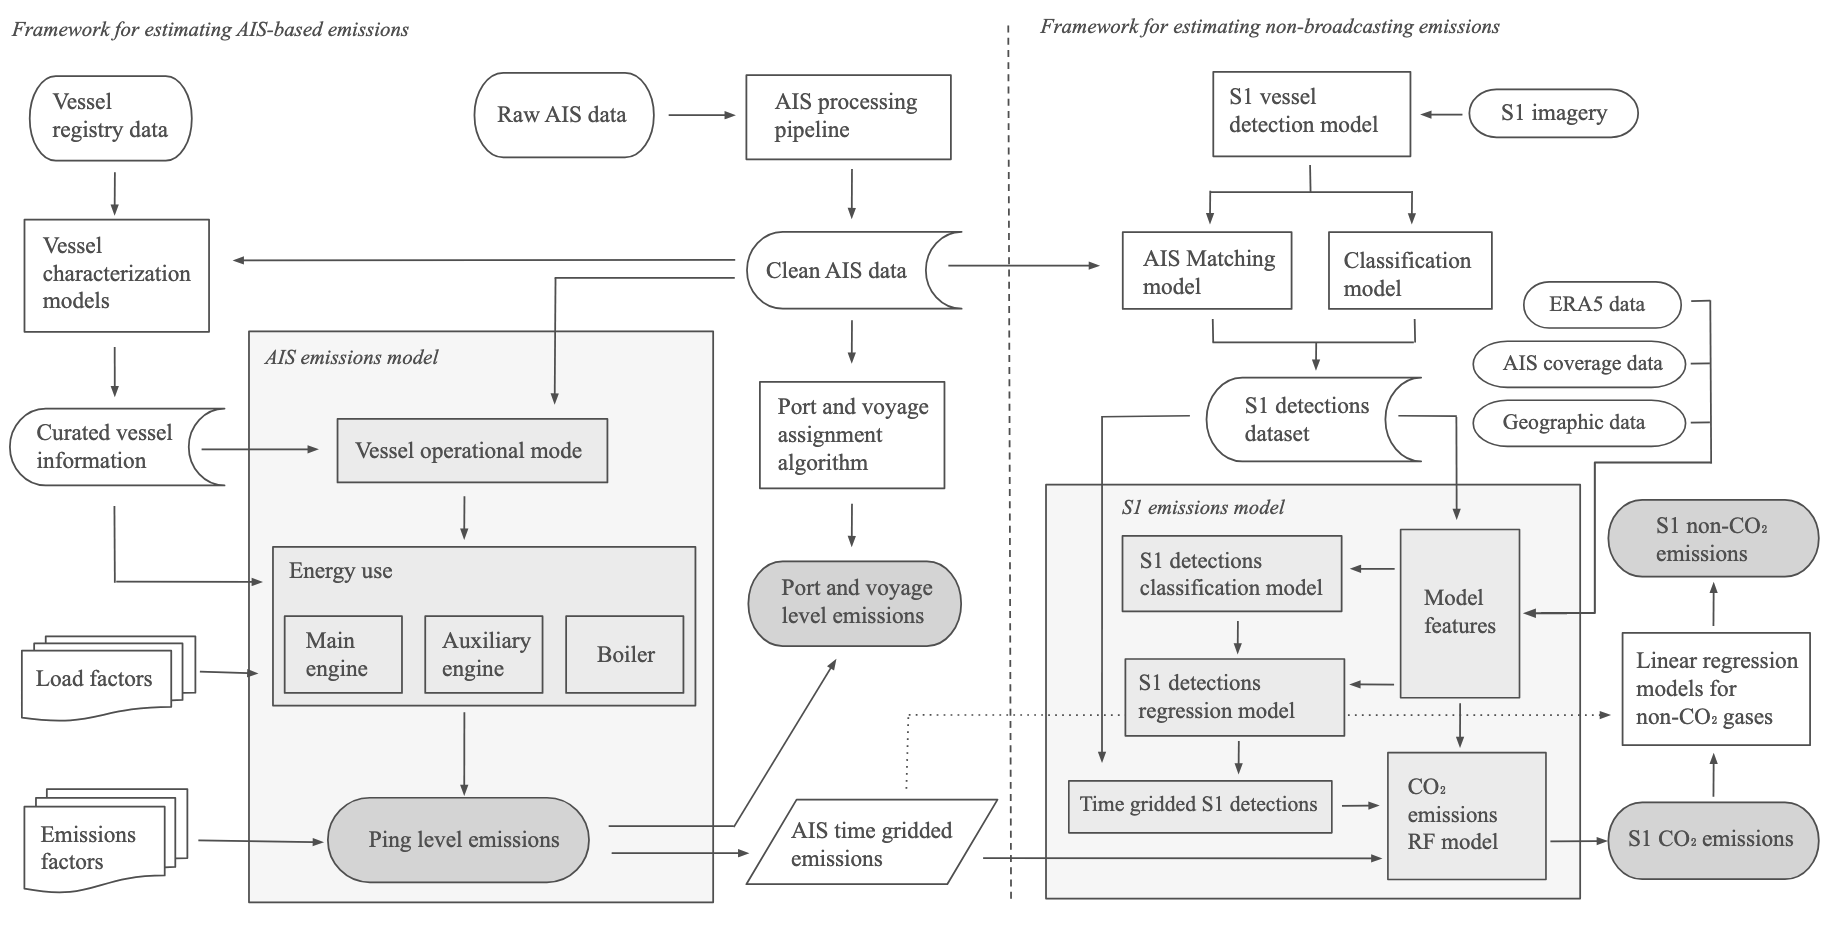
\includegraphics[width=\columnwidth]{figures/fig-framework-flowchart.png}
%DIFDELCMD <     %%%
\DIFdelendFL \DIFaddbeginFL 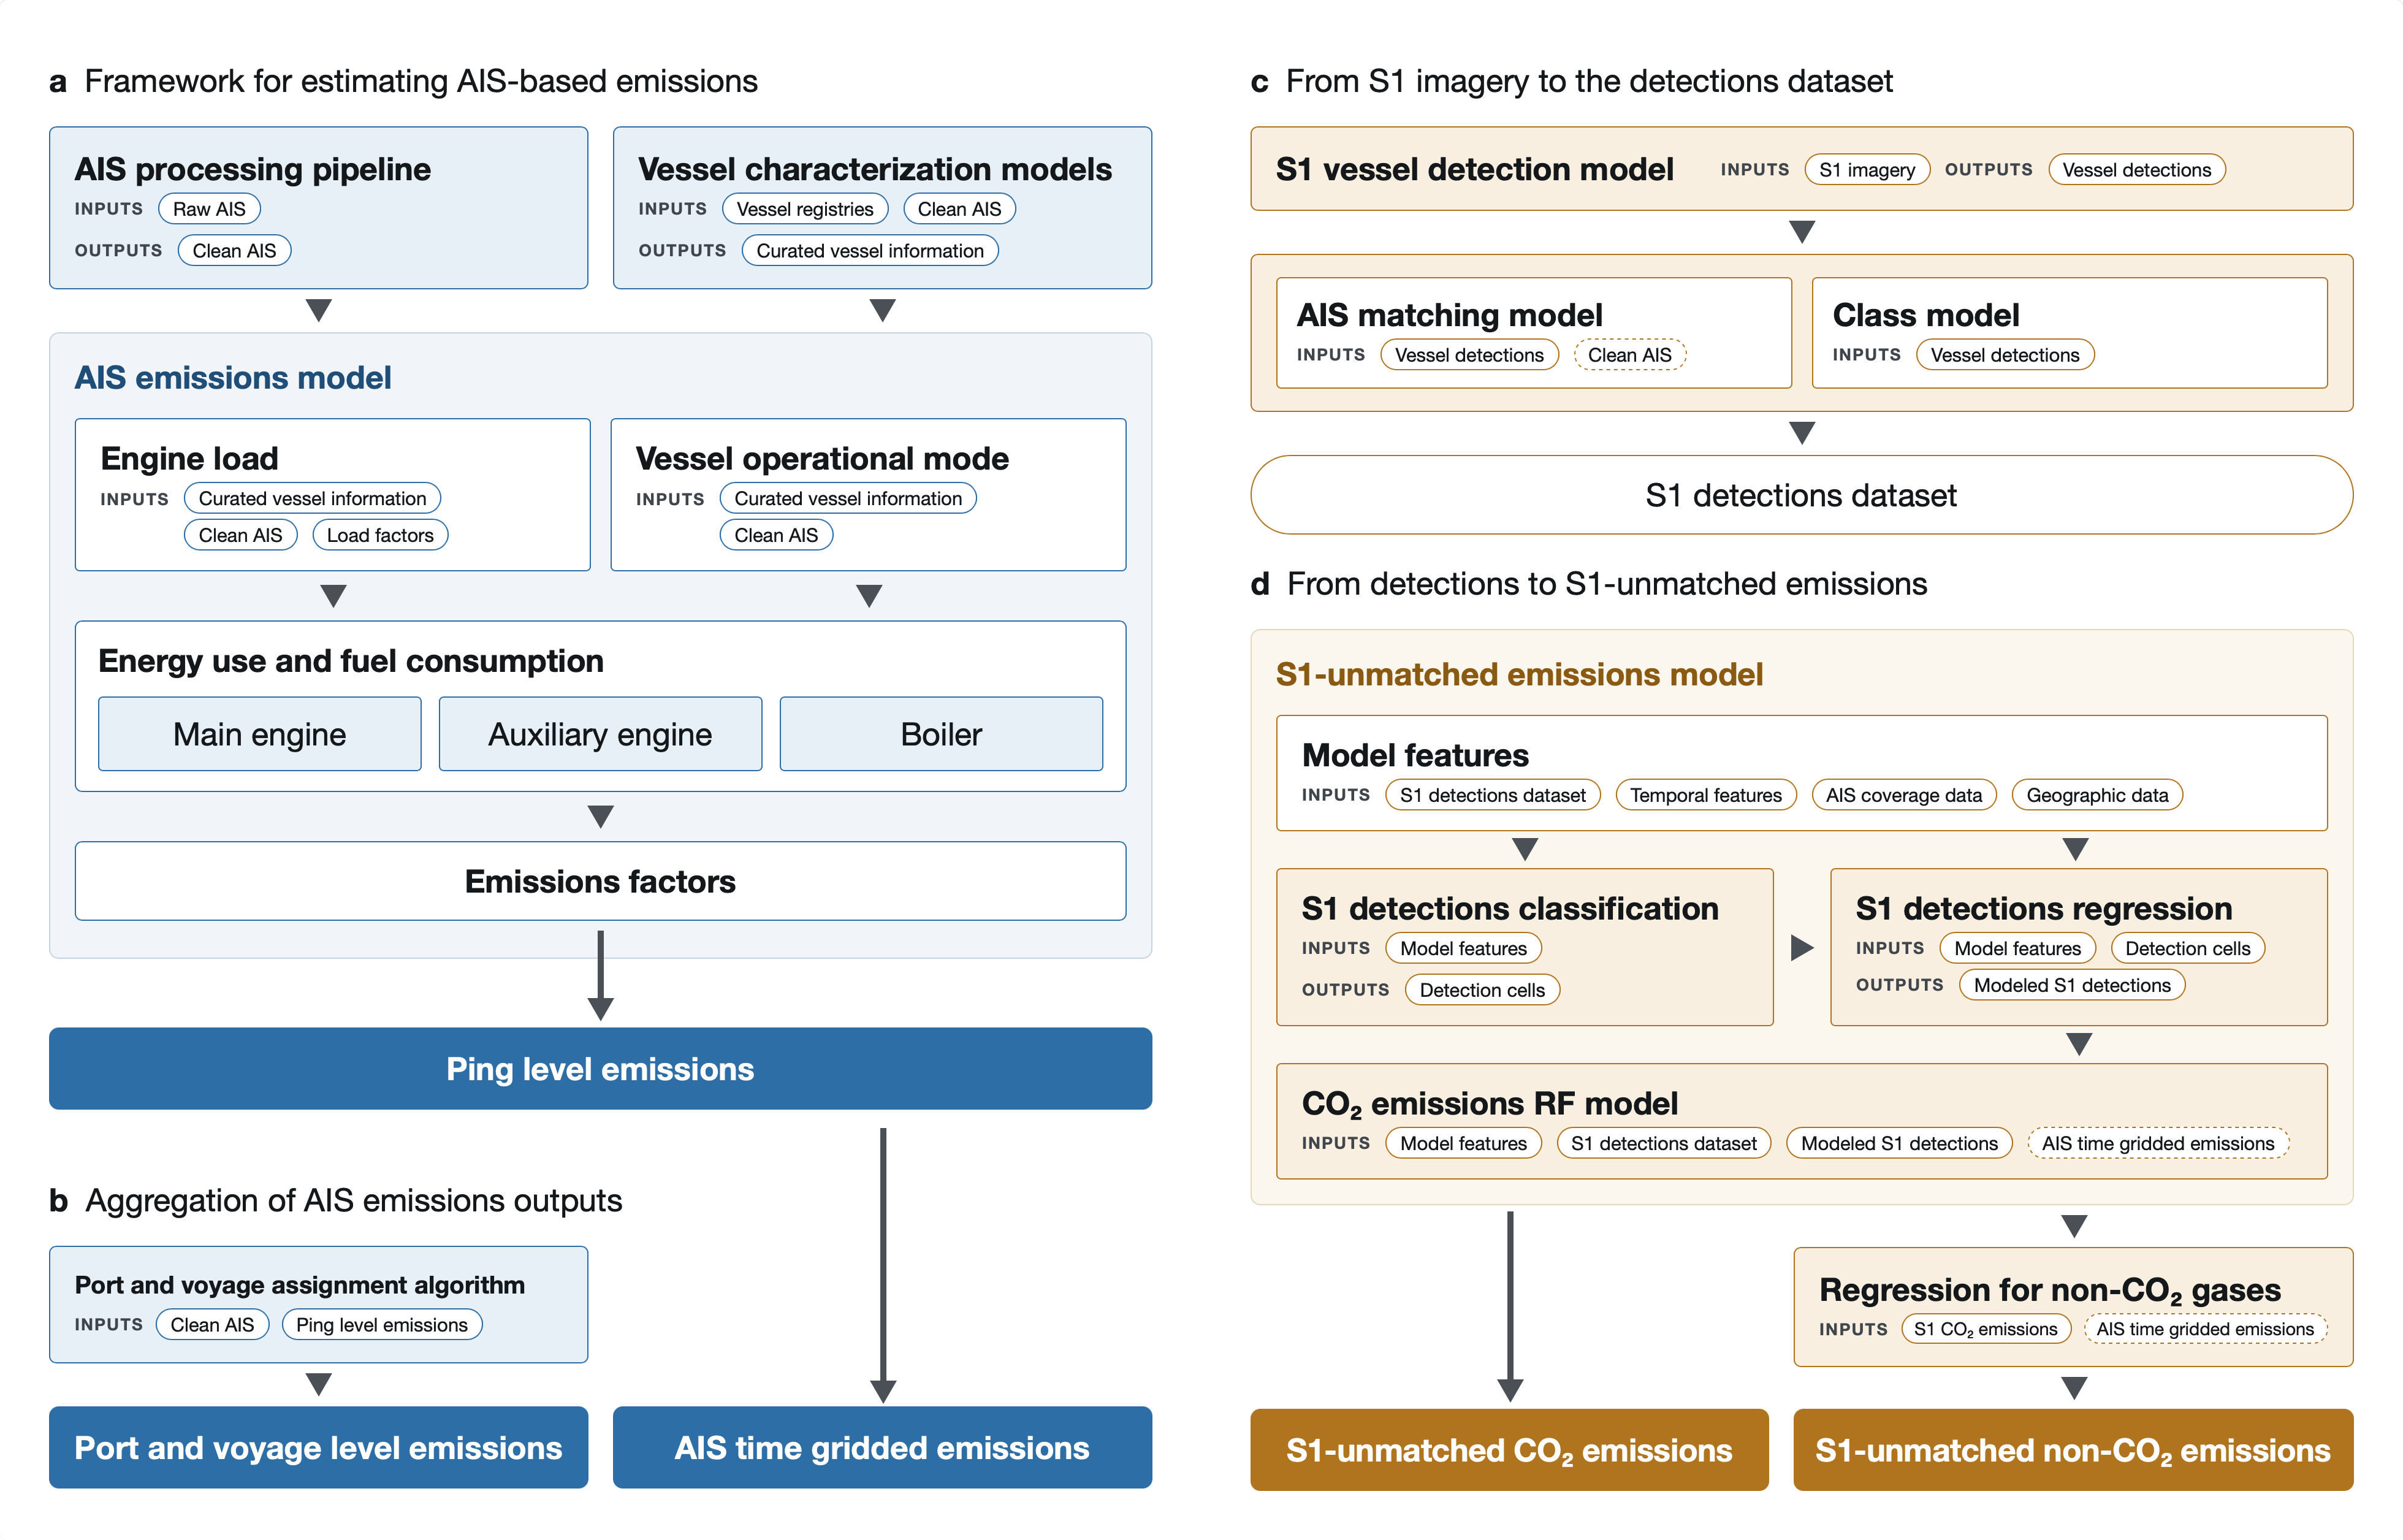
\includegraphics[width=\columnwidth]{figures/fig-framework-flowchart-simpler.png}
    \DIFaddendFL \caption{Conceptual flowchart for estimating emissions using the AIS-based emissions model and the \DIFdelbeginFL \DIFdelFL{non-broadcasting }\DIFdelendFL \DIFaddbeginFL \DIFaddFL{S1-unmatched }\DIFaddendFL emissions model.}
    \label{fig:gfw_emissions_framework_flowchart}
\end{figure}

The following sections describe our approaches for AIS-broadcasting vessels and \DIFdelbegin \DIFdel{non-broadcasting vessels}\DIFdelend \DIFaddbegin \DIFadd{for S1-unmatched vessel detections}\DIFaddend .

\subsection{AIS-broadcasting vessels}

\subsubsection{AIS data description}

\paragraph{AIS messages, port visits, and voyages}

We use individual AIS messages (pings) from the latest version of GFW’s AIS pipeline \DIFdelbegin \DIFdel{v3 \mbox{%DIFAUXCMD
\cite{gfw_version_3}}\hskip0pt%DIFAUXCMD
}\DIFdelend \DIFaddbegin \DIFadd{(`Version 5')}\DIFaddend , which parses, cleans, and augments raw AIS data \cite{kroodsma2018tracking}. \DIFaddbegin \DIFadd{GFW sources raw AIS from commercial providers of terrestrial (global coastal coverage by Spire Global 2017-2025 and Marine Traffic 2023-2025), satellite (near continuous global coverage, provided by ORBCOMM from 2017 to 2022, Spire Global from 2017 to 2025, and ExactEarth from 2023-2025) and, from 2022, dynamic AIS (Spire Global), covering both Class A and Class B transponders. Raw broadcasts are parsed and decoded from their encoded format into position messages, carrying location, speed and course, and static and voyage messages, carrying the identifiers and attributes a vessel reports about itself. Positions that are invalid, duplicated, or physically implausible are removed before any downstream processing.
}

\DIFaddend Since pings are grouped into segments using a segmenter \DIFdelbegin \DIFdel{\mbox{%DIFAUXCMD
\cite{kroodsma2018tracking,gfw_version_3}}\hskip0pt%DIFAUXCMD
}\DIFdelend \DIFaddbegin \DIFadd{\mbox{%DIFAUXCMD
\cite{kroodsma2018tracking}}\hskip0pt%DIFAUXCMD
}\DIFaddend , the time for a single ping represents the time since the previous ping in that segment; this value is typically small (the mean value is \DIFdelbegin \DIFdel{0.098 }\DIFdelend \DIFaddbegin \DIFadd{0.088 }\DIFaddend hours and the median value is \DIFdelbegin \DIFdel{0.049 }\DIFdelend \DIFaddbegin \DIFadd{0.046 }\DIFaddend hours, or about \DIFdelbegin \DIFdel{6 }\DIFdelend \DIFaddbegin \DIFadd{5 }\DIFaddend minutes and 3 minutes respectively), with virtually all pings representing $<$ 24 hours of activity. \DIFaddbegin \DIFadd{Because emissions are estimated over the interval each ping represents, the relevant quantity is the share of emissions these pings carry: 80.7\% of our AIS-based CO$_{2}$ emissions come from pings representing one hour or less of activity, 95.0\% from pings representing 12 hours or less, and effectively all from pings representing less than 24 hours (Fig. \ref{fig:fig-emissions-by-message-hour-threshold}, Table \ref{tab:emissions_by_message_hour_threshold}). }\DIFaddend The activity associated with individual pings form\DIFaddbegin \DIFadd{s}\DIFaddend  the basis of our ping-level \DIFdelbegin \DIFdel{AIS-broadcasting }\DIFdelend \DIFaddbegin \DIFadd{AIS-based }\DIFaddend emissions estimates, described below. These AIS messages come from a combination of satellite, terrestrial, and dynamic receivers (described in more detail \DIFdelbegin \DIFdel{under the section below `Trends in AIS receiver types' and }\DIFdelend \DIFaddbegin \DIFadd{in Supplementary Note \ref{sec:ais-receiver-types} and Supplementary }\DIFaddend Fig. \ref{fig:fig-annual-emissions-by-ais-receiver-type}, \DIFaddbegin \DIFadd{Supplementary }\DIFaddend Fig. \ref{fig:fig-annual-emissions-by-ais-receiver-type-top-flags}, \DIFaddbegin \DIFadd{Supplementary }\DIFaddend Fig. \ref{fig:fig-co2-emissions-change-map-by-receiver-type})

This dataset also classifies whether a fishing vessel is actively engaged in fishing activities at the ping level \cite{kroodsma2018tracking}. Finally, we leverage GFW's algorithm for detecting port visits \cite{gfw_anchorages_website}, allowing us to aggregate ping-level emissions to the vessel-specific port stays, as well as to vessel-specific port-to-port trips (both international and domestic). 

In all, we analyze AIS data for over \DIFdelbegin \DIFdel{880}\DIFdelend \DIFaddbegin \DIFadd{775}\DIFaddend ,000 AIS-broadcasting vessels, across \DIFdelbegin \DIFdel{94 }\DIFdelend \DIFaddbegin \DIFadd{119 }\DIFaddend billion individual timestamped AIS messages which are assigned to \DIFdelbegin \DIFdel{12.6 }\DIFdelend \DIFaddbegin \DIFadd{14.4 }\DIFaddend million international trips, \DIFdelbegin \DIFdel{96.7 }\DIFdelend \DIFaddbegin \DIFadd{112 }\DIFaddend million domestic trips, and \DIFdelbegin \DIFdel{83.3 }\DIFdelend \DIFaddbegin \DIFadd{96.4 }\DIFaddend million port visits that occurred between 2017 and \DIFdelbegin \DIFdel{2024.
}\DIFdelend \DIFaddbegin \DIFadd{2025.
}\DIFaddend 

\DIFaddbegin \begin{figure}[H]
    \centering
    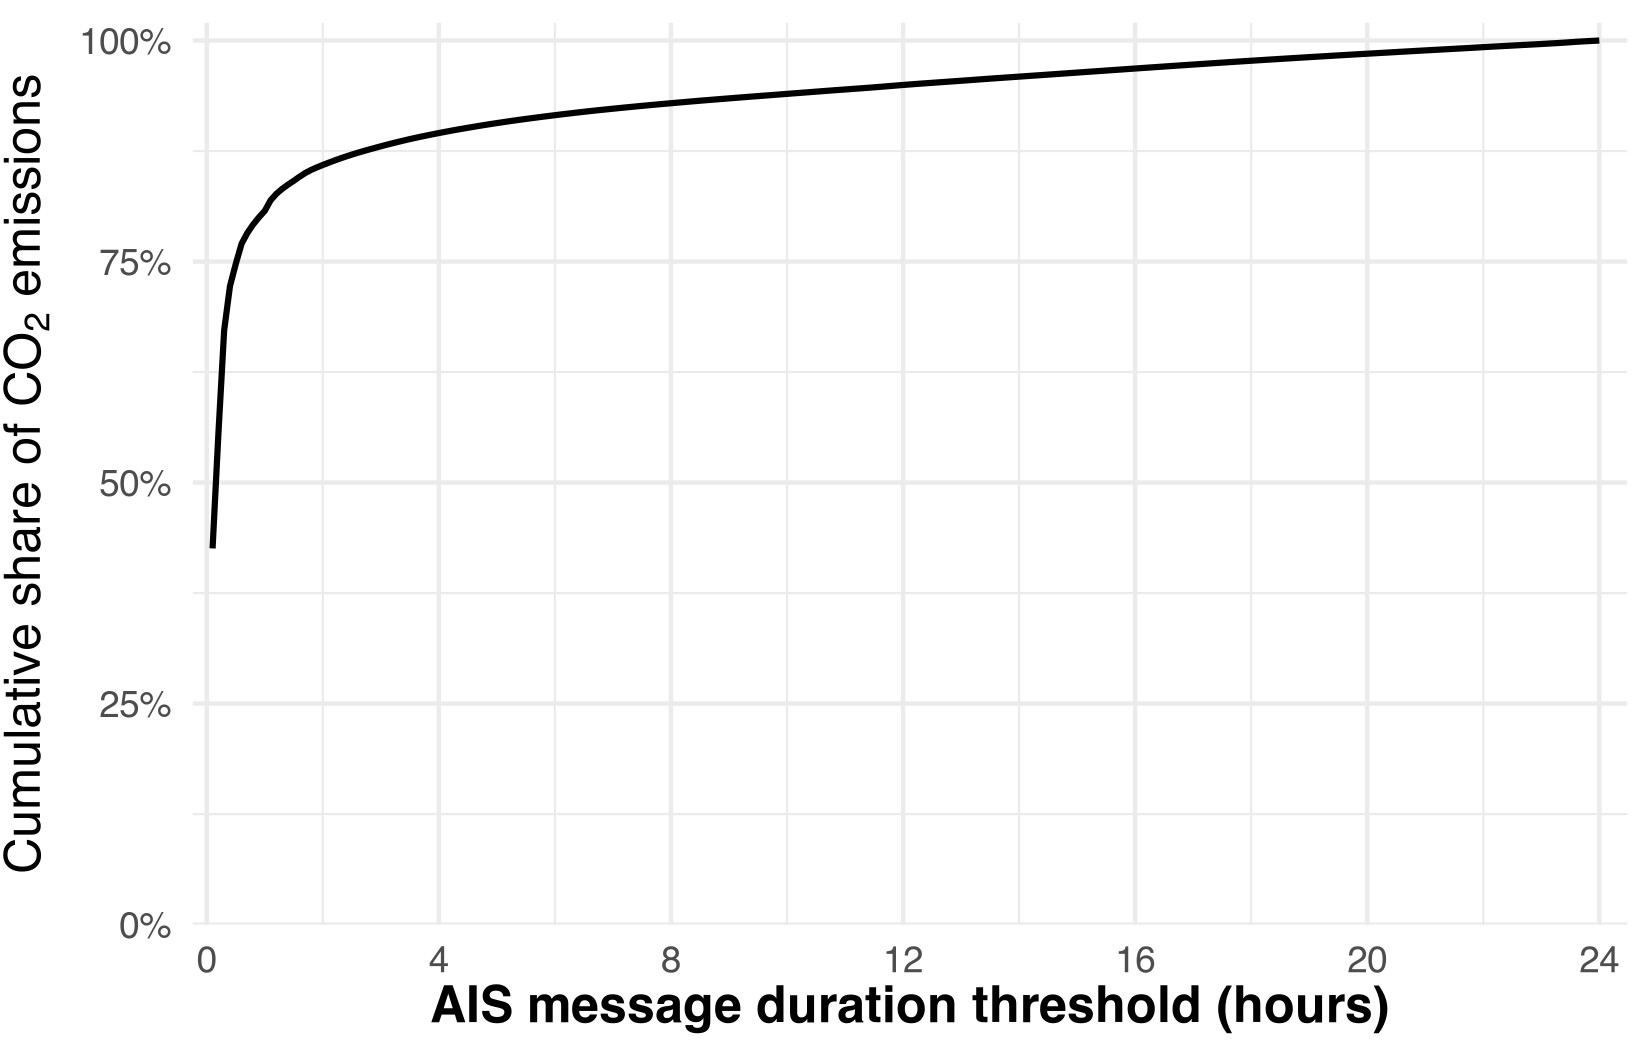
\includegraphics[width=\columnwidth]{figures/fig-emissions-by-message-hour-threshold-1.png}
    \caption{\DIFaddFL{Cumulative share of AIS-based CO$_{2}$ emissions attributable to pings whose assigned interval falls at or below a given threshold (using the full 2017 to 2025 time series of data). Each ping is assigned the time elapsed since the previous ping in its segment, and emissions are estimated over that interval, so long intervals are those over which activity is interpolated across a gap in the message stream rather than observed directly. Values at whole-hour thresholds are given in Table \ref{tab:emissions_by_message_hour_threshold}.}}
    \label{fig:fig-emissions-by-message-hour-threshold}
\end{figure}

\begin{table}[!h]
\centering
\caption{\label{tab:emissions_by_message_hour_threshold}\DIFaddFL{Cumulative AIS-based CO$_2$ emissions from messages whose assigned duration falls at or below each whole-hour threshold, 2017 to 2025. Shares are of all AIS-based CO$_2$ emissions, including that from messages with durations longer than 24 hours, so the at-or-below column need not reach 100\%. The above-threshold column is its complement: the share of emissions interpolated across gaps longer than the threshold. Figure \ref{fig:fig-emissions-by-message-hour-threshold} shows the full curve at 0.1-hour resolution.}}
\centering
\fontsize{8}{10}\selectfont
\begin{tabular}[t]{rrrr}
\toprule
Threshold (hours) & Cumulative CO$_2$ (million tonnes) & Share at or below & Share above\\
\midrule
1 & 7,086 & 80.73\% & 19.27\%\\
2 & 7,542 & 85.92\% & 14.08\%\\
3 & 7,727 & 88.04\% & 11.96\%\\
4 & 7,859 & 89.53\% & 10.47\%\\
5 & 7,958 & 90.66\% & 9.34\%\\
\addlinespace
6 & 8,036 & 91.55\% & 8.45\%\\
7 & 8,100 & 92.29\% & 7.71\%\\
8 & 8,155 & 92.91\% & 7.09\%\\
9 & 8,203 & 93.46\% & 6.54\%\\
10 & 8,247 & 93.96\% & 6.04\%\\
\addlinespace
11 & 8,291 & 94.46\% & 5.54\%\\
12 & 8,336 & 94.97\% & 5.03\%\\
13 & 8,378 & 95.45\% & 4.55\%\\
14 & 8,419 & 95.92\% & 4.08\%\\
15 & 8,459 & 96.37\% & 3.63\%\\
\addlinespace
16 & 8,499 & 96.83\% & 3.17\%\\
17 & 8,539 & 97.28\% & 2.72\%\\
18 & 8,576 & 97.71\% & 2.29\%\\
19 & 8,612 & 98.12\% & 1.88\%\\
20 & 8,646 & 98.51\% & 1.49\%\\
\addlinespace
21 & 8,679 & 98.88\% & 1.12\%\\
22 & 8,711 & 99.25\% & 0.75\%\\
23 & 8,743 & 99.61\% & 0.39\%\\
24 & 8,777 & 100.00\% & 0.00\%\\
\bottomrule
\end{tabular}
\end{table}
\FloatBarrier

\DIFaddend \paragraph{Vessel characteristics data}

\DIFdelbegin \DIFdel{We use vessel characteristics data from }\DIFdelend \DIFaddbegin \DIFadd{Translating AIS vessel activity data into emissions estimates requires information on numerous vessel-specific characteristics including vessel class, main engine power (kW), engine type, gross tonnage, maximum design speed (knots), vessel construction year, and engine operating speed (RPM). A key contribution of this work was therefore to refine and expand }\DIFaddend GFW's vessel \DIFdelbegin \DIFdel{metadata tables}\DIFdelend \DIFaddbegin \DIFadd{characteristics database to include accurate estimates of these attributes for all 775,000 AIS-broadcasting vessels included in our analysis}\DIFaddend . For each vessel, this \DIFdelbegin \DIFdel{includes}\DIFdelend \DIFaddbegin \DIFadd{information comes from}\DIFaddend : (1) official registry information when available \cite{park2023tracking}, or (2) when registry data are unavailable, \DIFdelbegin \DIFdel{algorithm-derived vessel characteristics including vessel class, main engine power, maximum design speed, and gross tonnage \mbox{%DIFAUXCMD
\cite{kroodsma2018tracking}}\hskip0pt%DIFAUXCMD
}\DIFdelend \DIFaddbegin \DIFadd{machine learning vessel characteristics models. The only exception to this is the proprietary S\&P Global Market Intelligence's Ships Dataset: due to data usage agreements, vessel characteristics from that particular database could only be used for model training, and could not be used directly by the emissions model or shared externally; for characteristics found only in that database, we therefore use modeled values, although they align very closely with those in the registry. Registry information is aggregated across a range of public and proprietary sources: IMO's GISIS; S\&P Global Market Intelligence's Ships Dataset; the national vessel registries of 19 flag states (the United States, Canada, Australia, Russia, the Republic of Korea, Norway, Indonesia, Iceland, Taiwan, the Faroe Islands, Spain, Panama, Peru, Ecuador, Seychelles, Malaysia, Belize, Papua New Guinea and Madagascar); the EU fleet register and FAO records; and the authorized-vessel lists of thirteen regional fisheries management organizations (ICCAT, IOTC, WCPFC, IATTC, SPRFMO, CCSBT, NEAFC, NPFC, GFCM, NAFO, SIOFA, CCAMLR and SEAFO) \mbox{%DIFAUXCMD
\cite{park2023tracking}}\hskip0pt%DIFAUXCMD
}\DIFaddend .


\DIFaddbegin \DIFadd{We briefly define these models here, and provide full details on training data, features, model performance, and known limitations in Sections \ref{sec:vessel-characteristics-models} and \ref{sec:vessel-characteristics-numeric-models}.
}

\DIFadd{Leveraging work pioneered by \mbox{%DIFAUXCMD
\cite{kroodsma2018tracking}}\hskip0pt%DIFAUXCMD
, GFW uses a primary vessel classification model to assign each AIS-broadcasting vessel into one of 32 vessel classes (Section \ref{sec:primary-vessel-class-model}). }\DIFaddend For vessels classified as \DIFdelbegin \DIFdel{"cargo" or "tankers" in }\DIFdelend \DIFaddbegin \DIFadd{`cargo' or `tankers' by }\DIFaddend GFW's \DIFdelbegin \DIFdel{metadata tables, we implement a random forest classification }\DIFdelend \DIFaddbegin \DIFadd{primary vessel classification model, we developed new gradient boosting }\DIFaddend sub-models that \DIFdelbegin \DIFdel{builds off }\DIFdelend \DIFaddbegin \DIFadd{refine }\DIFaddend the general vessel classification \DIFdelbegin \DIFdel{algorithm to differentiate }\DIFdelend \DIFaddbegin \DIFadd{into }\DIFaddend sub-categories \DIFdelbegin \DIFdel{that better align }\DIFdelend \DIFaddbegin \DIFadd{aligned }\DIFaddend with the Fourth IMO Greenhouse Gas Study vessel class types\DIFdelbegin \DIFdel{. The model is }\DIFdelend \DIFaddbegin \DIFadd{: five cargo categories (bulk carrier, container, general, refrigerated, and ro-ro) and four tanker categories (oil, chemical, liquefied gas, and other liquids) (Sections \ref{sec:cargo-submodel} and \ref{sec:tanker-submodel}). The sub-models are }\DIFaddend trained on port visit \DIFdelbegin \DIFdel{patterns from over 26}\DIFdelend \DIFaddbegin \DIFadd{history and vessel activity features, using labels derived from over 22}\DIFaddend ,000 vessels with known IMO vessel class types \DIFdelbegin \DIFdel{. The models are trained using labels derived from }\DIFdelend \DIFaddbegin \DIFadd{(}\DIFaddend S\&P Maritime StatCode5 categories\DIFdelbegin \DIFdel{. 
Features include vessel characteristics and activity metrics such as engine power, tonnage, average speed, AIS broadcasted shiptypes and sequences of port visits. Sequences of port visits were converted into usable model features using a Word2Vec model (50-dimensional embeddings with a context window of 10 anchorages). The cargosub-model classifies vessels into five categories: bulk carrier, container, general, refrigerated, and ro-ro (roll-on/roll-off for wheeled vehicle transport), achieving a weighted }\DIFdelend \DIFaddbegin \DIFadd{), and achieve weighted }\DIFaddend F1 \DIFdelbegin \DIFdel{score of 0.91. The tanker sub-model classifies vessels into three categories: chemical/oil, liquefied gas, and other liquids, achieving a weighted F1 score of 0.95}\DIFdelend \DIFaddbegin \DIFadd{scores of 0.91 (cargo) and 0.87 (tanker)}\DIFaddend . These refined cargo and tanker vessel class categories allow\DIFdelbegin \DIFdel{s}\DIFdelend  us to more accurately assign auxiliary engine power and boiler power to each vessel, which are based on lookup tables according to vessel class and size \cite{fourth2020greenhouse}. 

For the main engine power, gross tonnage, \DIFdelbegin \DIFdel{and }\DIFdelend maximum design speed estimates, \DIFaddbegin \DIFadd{vessel construction year, and engine operating speed, }\DIFaddend we develop separate random forest regression models \DIFaddbegin \DIFadd{(Section \ref{sec:vessel-characteristics-numeric-models})}\DIFaddend . All models are trained using the same features: inferred vessel classification scores, AIS self-reported shiptype messages, activity and location features derived from AIS usage, and values inferred from prior regression models. \DIFdelbegin \DIFdel{All models were trained on datasets of around 360,}\DIFdelend \DIFaddbegin \DIFadd{Each model was trained on between about 8,800 and 63,}\DIFaddend 000 labeled registry samples, \DIFdelbegin \DIFdel{with a holdout test set of 90, 000 for }\DIFdelend \DIFaddbegin \DIFadd{depending on the characteristic, with }\DIFaddend an 80/20 train-test split \DIFaddbegin \DIFadd{(Table \ref{tab:model-summary})}\DIFaddend . The main engine power, gross tonnage, \DIFdelbegin \DIFdel{and }\DIFdelend maximum design speed\DIFaddbegin \DIFadd{, engine RPM, and construction year }\DIFaddend regression models achieved traditional R$^{2}$ values \DIFdelbegin \DIFdel{exceeding 0.88, 0.83, and 0.74, }\DIFdelend \DIFaddbegin \DIFadd{of 0.93, 0.94, 0.86, 0.53, and 0.45 }\DIFaddend respectively.

The resulting vessel characteristics dataset contains the necessary metadata for estimating emissions using an AIS-based methodology for over \DIFdelbegin \DIFdel{880}\DIFdelend \DIFaddbegin \DIFadd{775}\DIFaddend ,000 active AIS-broadcasting vessels.

It should be noted that even when registries exist, vessel characteristics can be unrepresentative, particularly for fishing vessels. For instance, evidence from the European fishing sector suggests that vessels often use engines larger than those officially registered \cite{EC_EnginePower_2019}, while fraud also extends to reported vessel length and other characteristics \cite{ECA_FisheriesControl_2017}. Underreported main engine power would lead to an underestimation of AIS-based emissions from these vessels; and if underreported main engine power data are used for training models to infer main engine power, this may lead to a systematic underestimation of AIS-based emissions for vessels using inferred main engine power.

\DIFaddbegin \subsubsection{\DIFadd{Vessel class and characteristics models}}\label{sec:vessel-characteristics-models}

\DIFadd{Two families of machine learning models are used to estimate vessel classes and properties. Vessel class is determined by a combination of a broad, primary vessel class model and focused cargo and tanker sub-type models. Vessel properties are determined by six separate models used to estimate the following vessel characteristics: gross tonnage (GT), main engine power (kW), design speed (kn), year of build (year), engine speed (RPM), and engine type (class). Random forest classifiers are used for the primary vessel class and the engine type, and random forest regression models are used to estimate gross tonnage, engine power, design speed, year of build, and engine speed. Finally, gradient boosting classifiers are used for the cargo and tanker sub-type models. Details about each model can be found in the relevant subsections below.
}

\DIFadd{All models are trained on three categories of features derived from AIS information: inferred features (37), identity features (14), and activity features (13). The cargo and tanker sub-type models are trained on an additional 50 features derived from port visits. These features were built with Word2Vec (50 dimensions, window 10, minimum count 5) over each vessel's sequence of anchorage visits, from high-confidence port visits in the 365 days to 2025-06-01; a vessel's vector is the visit-weighted mean of the anchorages it used. Inferred features consist of vessel class neural network scores and neural network estimates for vessel length, tonnage, engine power, and crew size \mbox{%DIFAUXCMD
\cite{kroodsma2018tracking}}\hskip0pt%DIFAUXCMD
. Identity features include identification data broadcast through a vessel's AIS, such as the first digit and the broadcast vessel class. Activity features describe patterns in a vessel's AIS activity over time, such as fraction of active hours, average speed, distance from shore, etc.
}

\DIFadd{Training/test data for all models has an 80/20 split, and, except for the cargo and tanker sub-type models, is stratified by vessel class and the first digit of each MMSI to mitigate bias by vessel type or region. The number of training samples varied for each model as labeled data was available, with the primary GFW vessel class model having the most (510,486 training and 127,645 test samples). Test sample sizes available for all models are provided in the metrics Table \ref{tab:model-summary}. For each vessel characteristic model, Table \ref{tab:characteristic-availability} summarizes the percentage of vessels that had information already available from public sources, private sources, or for which inferred values from our models were used. 
}

\begin{table}[htbp]
  \centering
  \small
  \caption{\DIFaddFL{Performance for every model.
  Held-out values use the metric named in the }\emph{\DIFaddFL{Metric}} \DIFaddFL{column, so rows are comparable within a family but not across families.}}
  \label{tab:model-summary}
  \begin{tabular}{@{}llrrcc@{}}
    \toprule
    Model & Target & $n$ train & $n$ test & Metric & Held-out \\
    \midrule
    \multicolumn{6}{@{}l}{\textit{Classification models}} \\
    Vessel class        & 32 classes  & 510\,486  & 127\,645  & macro-F1 & 0.716 \\
    Engine type         & 4 classes  & 46\,108  & 11\,527  & macro-F1 & 0.550 \\
    Cargo sub-type      & 5 classes     & 11\,744 & 2\,939  & macro-F1 & 0.855     \\
    Tanker sub-type     & 4 classes     & 5\,903  & 1\,477  & macro-F1 & 0.712     \\
    \midrule
    \multicolumn{6}{@{}l}{\textit{Regression models}} \\
    Main engine power   & kW            & 13\,842  & 3\,542  & $R^2$    & 0.929 \\
    Gross tonnage       & GT            & 62\,636  & 15\,687  & $R^2$    & 0.944 \\
    Design speed        & knots         & 8\,808  & 2\,241  & $R^2$    & 0.861 \\
    Engine RPM          & rev$/$min     & 45\,868 & 11\,467  & $R^2$   & 0.533 \\
    Construction year   & year          & 45\,868  & 11\,467  & $R^2$    & 0.447 \\
    \bottomrule
  \end{tabular}
\end{table}


\begin{table}[htbp]
  \centering
  \small
  \caption{\DIFaddFL{Availability of vessel characteristics used in emissions modeling, by source.
  ``Inferred'' is the percentage of vessels for which the characteristic was not matched to any registry and was therefore inferred by our machine-learning models. ``Public Sources'' is the percentage sourced from any publicly available registry, including that maintained by IMO's GISIS (Global Integrated Shipping Information System). ``Private Sources'' is the percentage for which the characteristic is available from proprietary vessel databases, chiefly S\&P Global Market Intelligence's Ships Dataset and to a smaller extent non-public lists maintained by Global Fishing Watch. Under our data usage agreement, S\&P values are used only to train the machine-learning models, so wherever a characteristic is available only from S\&P, the emissions model uses the inferred value.}}\label{tab:characteristic-availability}
  \begin{tabular}{@{}lrrr@{}}
    \toprule
    Characteristic & Inferred (\%) & Public Sources (\%) & Private Sources (\%) \\
    \midrule
    Vessel Class      & 82.5 & 17.5 & 0.0 \\
    Gross Tonnage     & 85.4 & 14.3 & 0.2 \\
    Length            & 89.8 & 6.9  & 3.3 \\
    Main Engine Power & 92.5 & 3.1  & 4.4 \\
    Engine Type       & 93.9 & 0.0  & 6.1 \\
    Year of Build     & 94.0 & 0.0  & 6.0 \\
    Engine RPM        & 95.1 & 0.0  & 4.9 \\
    Design Speed      & 98.2 & 0.0  & 1.8 \\
    \bottomrule
  \end{tabular}
\end{table}
\FloatBarrier

\DIFadd{The primary GFW vessel class model, used to predict broad classes such as cargo, tanker, trawler, and gear, identifies the cargo and tanker vessels used in this analysis. Based on those classifications, the cargo and tanker sub-type models further refine those predictions into the more granular classes. Note that roughly 5\% of AIS messages are likely associated with non-vessel objects (such as buoys, offshore structures, FADs, etc). These objects are identified as their own vessel class `gear' by the primary GFW vessel class model, and are excluded from the emissions estimates in this paper. Residual misclassification between gear and vessels remains a source of uncertainty in both directions: non-vessel objects classified as vessels would add spurious emissions, while vessels classified as gear would be omitted (Section \ref{sec:primary-vessel-class-model}). Cargo and tanker sub-type labels are drawn from S\&P Global Market Intelligence's Ships Dataset, with StatCode5 levels 2--5 mapped to align with the fourth IMO Greenhouse Gas Study vessel class types, keeping only records that report a single MMSI so each label attaches to one vessel identity.
}


\subsubsection{\DIFadd{Primary GFW vessel class model}}\label{sec:primary-vessel-class-model}

\paragraph{\DIFadd{Target}} 
\DIFadd{The primary GFW vessel class model made vessel class predictions at the MMSI level for 1.8M active, AIS-broadcasting vessels. This is the full set of MMSIs scored by the model, and is therefore broader than the fleet carried into the emissions analysis: it includes non-vessel objects and vessels active outside our study period, both of which are excluded downstream. Vessels are assigned a unique class, separated into fishing, non-fishing, and gear, where gear refers to non-vessel AIS-enabled objects.
The final assigned vessel class follows a hierarchy determined by the model’s score for that class, where low-scoring classes get a final assignment at a coarser level. For example, a low-scoring “tanker” might be assigned a final vessel class “non-fishing”.
}


\paragraph{\DIFadd{Training data}}
\DIFadd{The primary GFW vessel class model makes use of all inferred, identity, and activity features described above. Labels are drawn from clean, aggregated registry data, ensuring that re-used MMSIs and MMSIs with conflicting classes by registry are dropped from training. 
510,486 vessels with aggregated registry information were used to train the model, with a holdout set of 127,645 for testing.
}


\paragraph{\DIFadd{Performance}}
\DIFadd{The model achieves an accuracy (equal to weighted recall) of 98.57\%, with weighted precision and F1 both at 98.7\%. Macro-averaged precision, recall, and F1 are 87.8\%, 64.8\%, and 71.6\%, respectively. The gap between weighted and macro reflects a class imbalance, with rare classes performing worst.
Cargo and tanker vessels are well-represented in the training data and perform well individually. Cargo achieves an F1 score of 97.0\%, and tanker reaches an F1 score of 95.6\%.
}

\paragraph{\DIFadd{Key predictive features}}
\DIFadd{The top features are determined using the Gini index, an imperfect but useful measure. Transmitted shiptype unavailable: 0.10, median speed: 0.09, most common AIS class: 0.08, transmitted shiptype cargo: 0.07, neural net passenger vessel score: 0.06, neural net gear score: 0.06, neural net cargo score: 0.05.
}

\paragraph{\DIFadd{Interpretability}}
\DIFadd{The feature importances are relatively spread out across different training features, with the most indicative feature whether or not the vessel broadcasts a shiptype. This makes sense, as vessel class is gear-dominated, and gear typically does not broadcast a shiptype. Other features, such as median speed, AIS class, and cargo shiptype, indicate a combination of vessel behavior and AIS information itself, while the neural net scores for specific classes show the propagation of one model's predictions into the next.
}


\paragraph{\DIFadd{Overfitting controls and known weaknesses}}
\DIFadd{The model uses regularized hyperparameters (}\texttt{\DIFadd{n\_estimators=300}}\DIFadd{, }\texttt{\DIFadd{max\_depth=35}}\DIFadd{, }\texttt{\DIFadd{min\_samples\_leaf=10}}\DIFadd{, }\texttt{\DIFadd{min\_samples\_split=20}}\DIFadd{) rather than an unconstrained forest to balance accuracy against model size. In order to mitigate overfitting or regional bias, the 80/20 split in the train/test data is stratified by vessel class and MMSI region, and the label-exclusion rules reduce noisy or duplicated MMSI from training. The tight cross-validation variance ($±$0.05\% accuracy across folds) suggests the model isn’t overfit to a particular split.
}

\DIFadd{Despite the training data stratification, high-volume classes such as gear and cargo perform very well, while rarer classes where limited data is available struggle significantly. Larger classes, particularly gear, may be over-classified. Because the model applies a score threshold to mitigate low-scoring, incorrect classifications, some correctly classified vessels may end up assigned too broad a label.
}

\DIFadd{As the vessel sub-type models rely on the output of the primary vessel classification model predictions, biases and errors are propagated from this model to the next. This effect similarly happens between the neural net scores and the primary GFW vessel class model.
}


\subsubsection{\DIFadd{Cargo sub-type model}}
\label{sec:cargo-submodel}

\paragraph{\DIFadd{Target}}

\DIFadd{One of five cargo sub-types (bulk carrier, container, general cargo, refrigerated cargo, ro-ro cargo), for 186\,689 vessels the primary vessel class model classified as cargo.
}

\paragraph{\DIFadd{Training data}}

\DIFadd{11\,744 vessels with S\&P registry sub-types: bulk carrier 5\,201; general cargo 3\,200; container 2\,166; ro-ro 1\,100; refrigerated 77.
}

\paragraph{\DIFadd{Performance}}

\DIFadd{Accuracy 90.5\%; macro-F1 85.5\%; weighted F1 90.5\%. Per-class F1: bulk carrier 94.3, container 93.9, general cargo 84.7, ro-ro 84.6, refrigerated 70.3.
}

\paragraph{\DIFadd{Key predictive features}}

\DIFadd{Importance is the loss in held-out macro-F1 when a feature is permuted, used in place of the Gini index, which is undefined for the gradient boosting models used here. Anchorage embeddings, 50 dimensions permuted together: 0.220. Vessel class neural network scores, 33 permuted together: 0.157. Top speed (95th percentile): 0.029.
}

\paragraph{\DIFadd{Interpretability}}

\DIFadd{Vessel class neural network scores form a substantial part of this model's classification skill, indicating it is potentially inherited from the neural network rather than learned from vessel behavior.
}

\paragraph{\DIFadd{Overfitting controls and known weaknesses}}

\DIFadd{Gradient boosting classifiers with early stopping on a held-out internal validation split, rather than a fixed number of boosting iterations. Unlike the primary model, the train/test split here is stratified by sub-type only rather than by MMSI region, with the split fixed by an MMSI hash so it is stable as data is added.
}

\DIFadd{Refrigerated cargo has 77 training vessels; its F1 of 70.3 is indicative only. Ro-ro and general cargo are the main confusion pair among the well-populated classes: 17\% of ro-ro vessels are predicted as general cargo. General cargo is 27\% of the training set but 66\% of predictions, so the model is likely extrapolating beyond its training mix.
}

\DIFadd{Errors in the primary model are also inherited: a vessel it misclassifies is assigned a sub-type from the wrong class. Labels exist only for S\&P-registered, single-MMSI vessels, and 4.5\% of training vessels have no port visit features at all.
}

\subsubsection{\DIFadd{Tanker sub-type model}}
\label{sec:tanker-submodel}

\paragraph{\DIFadd{Target}}

\DIFadd{One of four tanker sub-types (oil, chemical, liquefied gas, other liquids), for 43\,530 vessels the primary vessel class model classified as tanker.
}

\paragraph{\DIFadd{Training data}}

\DIFadd{5\,903 vessels with S\&P registry sub-types: oil 2\,664; chemical 2\,015; liquefied gas 1\,188; other liquids 36.
}

\paragraph{\DIFadd{Performance}}

\DIFadd{Accuracy 87.5\%; macro-F1 71.2\%; weighted F1 87.4\%. Per-class F1: liquefied gas 91.8, oil 88.6, chemical 84.3, other liquids 20.0.
}

\paragraph{\DIFadd{Key predictive features}}

\DIFadd{Top speed (95th percentile): 0.169. Anchorage embeddings, 50 dimensions permuted together: 0.145. Vessel class neural network scores, 33 permuted together: 0.061. Average distance traveled per trip: 0.030.
}

\paragraph{\DIFadd{Interpretability}}

\DIFadd{Top speed carries more importance in this model than any other single feature. This makes the model easy to explain, but it also means it leans on a single behavioral signal that degrades wherever AIS coverage is patchy.
}

\paragraph{\DIFadd{Overfitting controls and known weaknesses}}

\DIFadd{Gradient boosting classifiers with early stopping on a held-out internal validation split. As with the cargo model, the train/test split is stratified by sub-type only, and the same label-coverage limits and inheritance of errors from the primary model apply.
}

\DIFadd{Performance for }\emph{\DIFadd{other liquids}} \DIFadd{is poor: recall 11.1\%, with 89\% of those vessels predicted as oil. With 45 labeled vessels in total the class does not have enough signal to be separated. Oil and chemical tankers are often confused with each other: 13\% of chemical vessels are called oil and 10\% the reverse. 5.6\% of training vessels have no port visit features at all.
}


\subsubsection{\DIFadd{Other vessel characteristics models}}\label{sec:vessel-characteristics-numeric-models}

\paragraph{\DIFadd{Targets}}

\DIFadd{Continuous numeric vessel characteristics (main engine power, gross tonnage, design speed, construction year, and engine RPM) are estimated using random forest regression models, while the categorical engine type value is estimated using a random forest classifier. All models make predictions at the MMSI level for the same 1.8M active, AIS-broadcasting vessels scored by the primary vessel class model.
}

\paragraph{\DIFadd{Training data}}

\DIFadd{All models make use of the inferred, identity, and activity features described above. Labels are drawn from clean, aggregated registry data, ensuring that re-used MMSIs and MMSIs with conflicting classes by registry are dropped from training.
The engine power model had a training set of 13,842 samples, the gross tonnage model had a training set of 62,636 samples, the design speed model had a training set of 8,808 samples, the construction year and engine RPM models had a training set of 45,868 samples, and the engine type model had a training set of 46,108 samples.
}

\paragraph{\DIFadd{Performance}}
\\
\textit{\DIFadd{Engine power model}}
\\
\DIFadd{The engine power model achieved an R$^2$ of 0.929 with a mean absolute error of 548.71 kW and a mean absolute percentage error of 43.8\%.
}\\
\\
\textit{\DIFadd{Tonnage model}}
\\
\DIFadd{The tonnage model achieved an R$^2$ of 0.944 with a mean absolute error of 2,830.15 GT and a mean absolute percentage error of 209.6\%.
}\\
\\
\textit{\DIFadd{Design speed model}}
\\
\DIFadd{The design speed model achieved an R$^2$ of 0.861 with a mean absolute error of 0.82 kn and a mean absolute percentage error of 4.9\%.
}\\
\\
\textit{\DIFadd{Year-of-build model}}
\\
\DIFadd{The year-of-build model achieved an R$^2$ of 0.447 with a mean absolute error of 6.68 and a mean absolute percentage error of 0.3\%.
}\\
\\
\textit{\DIFadd{Engine RPM model}}
\\
\DIFadd{The engine RPM model achieved an R$^2$ of 0.533 with a mean absolute error of 360.56 and a mean absolute percentage error of 33.2\%.
}\\
\\
\textit{\DIFadd{Engine type model}}
\\
\DIFadd{Accuracy of 99.08\%; macro-F1 55.0\%; weighted F1 99.1\%. Per class F1: oil 99.5\%, gas 61.7\%, turbine 57.1\%, reciprocating 0.00.
}

\paragraph{\DIFadd{Key predictive features}}

\textit{\DIFadd{Engine power model}}
\\
\DIFadd{Average engine power inferred by neural network: 0.535. Top speed (95th percentile): 0.149. Average tonnage inferred by neural network: 0.104.
}\\
\\
\textit{\DIFadd{Tonnage model}}
\\
\DIFadd{Average tonnage inferred by neural network: 0.626. Fraction of hours spent at port: 0.0968. Average distance traveled per trip: 0.041.
}\\
\\
\textit{\DIFadd{Design speed model}}
\\
\DIFadd{Top speed (95th percentile): 0.609. Median speed: 0.054. Neural network supply vessel score: 0.051.
}\\
\\
\textit{\DIFadd{Year-of-build model}}
\\
\DIFadd{Average engine power inferred by the neural network: 0.162. First digit of the MMSI code: 0.101. Average tonnage inferred by the neural network: 0.063.
}\\
\\
\textit{\DIFadd{Engine RPM model}}
\\
\DIFadd{Average gross tonnage inferred by the neural network: 0.310. Average length inferred by the neural network: 0.093. Average percentage of self-identified shiptype messages as fishing: 0.074.
}\\
\\
\textit{\DIFadd{Engine type model}}
\\
\DIFadd{Top speed (95th percentile): 0.096. Neural network patrol vessel score: 0.080. Average engine power inferred by the neural network: 0.062.
}

\paragraph{\DIFadd{Interpretability}}

\DIFadd{Both the engine power and the tonnage predictions are largely driven by the neural network's inferred values, indicating that these models are refining existing predictions.
}\\
\DIFadd{The design speed predictions are most heavily reliant on the vessel's top speed and median speed, which makes intuitive sense as the two act as a proxy for design speed.
}\\
\DIFadd{The year-of-build predictions are less singularly reliant on one strong signal, but are driven the most by the neural network's inferred engine power and the first digit of the MMSI code. The latter likely acts as a proxy for build/registration era for each flag state.
}\\
\DIFadd{The engine RPM predictions are largely weighted by physical characteristics of the vessel, but similarly less reliant on a single feature. The physical characteristics describing a vessel likely act as a proxy for RPM, while the self-identified shiptype likely distinguishes fishing and non-fishing vessel properties.
}\\
\DIFadd{The top features for engine type predictions are much more diffuse, suggesting that no single feature strongly separates engine types and the model relies on combinations of weaker signals.
}

\paragraph{\DIFadd{Overfitting controls and known weaknesses}}
\DIFadd{To mitigate overfitting, all models are trained with a fixed random seed and a train/test split stratified by vessel class and first-digit MMSI. The engine type model additionally used class-weight balancing to counteract severe class imbalance in the training labels. However, because the engine type labels are so heavily skewed towards oil engines, the model only performs reliably for that class, and semi-reliably for gas. As higher volume data becomes available for a greater diversity of engine types, future models will be more sophisticated and better at predicting the less represented types. 
}

\DIFadd{The year-of-build model has a 6-7 year mean error, suggesting that it is useful for predicting general build era up to around a decade, but not reliable for year-by-year predictions. The engine RPM model has mean error of 360 revolutions per minute, indicating that it can capture very broad patterns but with more relative error than the year-of-build model.
The engine power, tonnage, and design speed models all show the same pattern: performance is strongest in the mid-range of each variable and degrades substantially at the extremes, where training data is sparse.
}

\DIFaddend \subsubsection{Emissions model for AIS-broadcasting vessels}

We adapted our AIS-based model from the methodologies described in the 2017 ICCT study on global shipping emissions \cite{olmer2017greenhouse} and the 2020 IMO Fourth Greenhouse Gas Study \cite{fourth2020greenhouse}, making modifications to better align with the structure and characteristics of our data sets. From a high-level, we: 
\DIFdelbegin \DIFdel{1) determine }\DIFdelend \DIFaddbegin 

\DIFadd{1. Determine }\DIFaddend the main engine energy use, auxiliary engine energy use, and boiler energy use for each individual AIS message based on dynamic vessel movement and static vessel characteristic data
\DIFdelbegin \DIFdel{; 2)}\DIFdelend \DIFaddbegin 

\DIFadd{2. Determine fuel consumption for each individual AIS message based on dynamic vessel movement and static vessel characteristic data.
}

\DIFadd{3. For the seven pollutants whose emissions factors depend on energy use (CH$_{4}$, CO, N$_{2}$O, NO$_{x}$, VOCs, PM$_{2.5}$, and PM$_{10}$), }\DIFaddend multiply the engine and boiler energy use numbers by pollutant- and engine-type-specific emissions factors in order to determine the amount of emissions for \DIFdelbegin \DIFdel{six pollutants }\DIFdelend \DIFaddbegin \DIFadd{each pollutant }\DIFaddend associated with the engines and boiler for each ping\DIFdelbegin \DIFdel{; 3)add }\DIFdelend \DIFaddbegin \DIFadd{.
}

\DIFadd{4. For the two pollutants whose emissions factors depend on fuel consumption (CO$_{2}$ and SO$_{x}$), for each ping multiply the fuel consumption by the appropriate pollutant- and engine-type-specific emissions factors in order to determine the amount of emissions for each pollutant and ping.
}

\DIFadd{5. Add }\DIFaddend up the emissions for \DIFdelbegin \DIFdel{these six pollutants}\DIFdelend \DIFaddbegin \DIFadd{each of the nine pollutants, from }\DIFaddend across the engines and boiler, to obtain the total emissions for each ping and each of these \DIFdelbegin \DIFdel{six pollutants; 4) estimate emissions for three additional pollutants that do not detailed information on emissions factors by simply multiplying the total CO$_{2}$ emissions for each ping by a conversion factor \mbox{%DIFAUXCMD
\cite{mayesshipping}}\hskip0pt%DIFAUXCMD
. 
We should note that we }\DIFdelend \DIFaddbegin \DIFadd{nine pollutants. 
}

\DIFadd{We }\DIFaddend focus our analysis \DIFaddbegin \DIFadd{purely }\DIFaddend on estimating emissions associated with fuel combustion in the main engine, auxiliary engine, and boiler; we do not include  methane slip on vessels that use liquefied natural gas, or other non-combustion fugitive emissions associated with refrigeration, cooling, or venting of VOCs from vessels that transport liquid cargo such as oil and chemicals.

Main engine energy use is estimated based on the time between each AIS ping (hours), the main engine power from the vessel characteristics dataset, and a load factor used to adjust the estimate. The load factor is the product of four coefficients: (1) a weather correction factor (represented by distance to shore, a proxy that can be observed from AIS data\DIFdelbegin \DIFdel{- vessel }\DIFdelend \DIFaddbegin \DIFadd{; vessels }\DIFaddend operating beyond 5 nautical miles from shore receive a value of 1.15; vessels operating within 5 nautical miles receive a value of 1.1 \cite{fourth2020greenhouse}); (2) a hull fouling correction factor, which causes resistance in the water (set at 1.07 according to \cite{olmer2017greenhouse}); \DIFdelbegin \DIFdel{and }\DIFdelend (3) a vessel draft correction factor (set at 0.85, the emissions-weighted average draft correction factor from \cite{fourth2020greenhouse}\DIFaddbegin \DIFadd{)}\DIFaddend ; and (4) a cubic term of vessel speed divided by  the vessel's maximum design speed. To determine the vessel speed associated with each AIS message, we use either: 1) the transmitted instantaneous speed associated with the AIS message if less than an hour has passed since the last message was transmitted; or 2) the implied speed for messages for which more than an hour has passed since the previous message (calculated as the distance traveled divided by the elapsed time between the two messages). We apply this hierarchy since implied speed can be imprecise for short time intervals between pings due to signal latency; meanwhile, instantaneous speed can be unrepresentative of longer time intervals between pings, in which case implied speed is more representative. Following \cite{coello2015ais, sala2018economics}, for fishing vessels we adjust the main engine load factor so that it falls between 0.2 and 0.9, and assign a main engine load factor of 0.75 to trawlers and dredge fishing vessels that are actively fishing due to the energy intensive nature of their fishing operations. 

In accordance with \cite{fourth2020greenhouse}, our model also accounts for differences in auxiliary engine \DIFdelbegin \DIFdel{power }\DIFdelend energy use and boiler energy use depending on the vessel \DIFaddbegin \DIFadd{type, as well as the vessel}\DIFaddend ’s operational phase—whether it is at berth, at anchor, maneuvering, or at sea. These phases are identified using AIS speed, distance to port, and distance to the coast. Power outputs for auxiliary engines and boilers, based on vessel class and size, are extracted from \cite{fourth2020greenhouse} and are applied accordingly for each phase. 


\DIFdelbegin \DIFdel{After calculating energy use, we apply pollutant-specific emission factors to }\DIFdelend \DIFaddbegin \DIFadd{Fuel consumption, for each of }\DIFaddend the main engine, auxiliary engine, and boiler\DIFdelbegin \DIFdel{for six GHGs and pollutants (}\DIFdelend \DIFaddbegin \DIFadd{, is next calculated as energy use multiplied by specific fuel consumption (SFC). The SFC for each of the main engine, auxiliary engine, and boiler is based on engine type and fuel type  \mbox{%DIFAUXCMD
\cite{fourth2020greenhouse}}\hskip0pt%DIFAUXCMD
. Our vessel characteristics database includes broad categories of engine type (oil, gas, or turbine), as well as engine operating speed which allows us to differentiate between high speed diesel, medium speed diesel, and low speed diesel. Since our vessel characteristics database does not specify fuel type for each vessel, we use the average values from across fuel types for each type of engine. For the main engine, SFC is further modulated based on engine load: engines operating at low loads below 20\% operate inefficiently, and therefore consume more fuel for the same amount of energy output  \mbox{%DIFAUXCMD
\cite{olmer2017greenhouse, fourth2020greenhouse}}\hskip0pt%DIFAUXCMD
. For the two pollutants whose emissions factors depend on fuel use (}\DIFaddend CO\DIFdelbegin \DIFdel{$_{2}$, CH$_{4}$, CO, NO$_{x}$, SO$_{x}$, N}\DIFdelend $_{2}$ \DIFdelbegin \DIFdel{O), following \mbox{%DIFAUXCMD
\cite{olmer2017greenhouse}}\hskip0pt%DIFAUXCMD
. These factors are each averaged from across the relevant pollutant factors associated with SSD, MSD, and HSD enginetypes, which together represent approximately 98\% of vessels engines \mbox{%DIFAUXCMD
\cite{fourth2020greenhouse}}\hskip0pt%DIFAUXCMD
. To get total emissions for each AIS message (i.e., emissions from the previous ping in a segment to the current one), we sum emissions from both engines and boilers.
For }\DIFdelend \DIFaddbegin \DIFadd{and SO$_{x}$), these emissions are therefore directly adjusted during inefficient low load operation.
}


\DIFadd{For the other seven pollutants whose emissions factors depend instead directly on energy use (CH$_{4}$, CO, N$_{2}$O, NO$_{x}$, }\DIFaddend VOCs, PM$_{2.5}$, and PM$_{10}$\DIFdelbegin \DIFdel{, which do not have as detailed information on emissions factors, we instead multiply the CO$_{2}$ emissions by pollutant-specific conversion factors \mbox{%DIFAUXCMD
\cite{mayesshipping}}\hskip0pt%DIFAUXCMD
. We also apply main engine }\DIFdelend \DIFaddbegin \DIFadd{), we account for inefficient main engine operation during low load by using the low load correction factors provided by \mbox{%DIFAUXCMD
\cite{epa2020ports} }\hskip0pt%DIFAUXCMD
(which were subsequently adopted by \mbox{%DIFAUXCMD
\cite{fourth2020greenhouse}}\hskip0pt%DIFAUXCMD
). Low-load correction factors are provided in the EPA report as a table showing a range from $\le 2\%$ through $\ge 20\%$ in incremental steps of 1\%. To use these, we apply the following hierarchy: if our estimated main engine load is $\le 2\%$, we apply the correction factor corresponding to $\le 2\%$; if our estimated main engine load is $\ge 20\%$, we apply a correction factor of 1; if our estimated main engine load corresponds perfectly to one of the incremental percentage steps in the table, we apply the corresponding  correction factor; finally, if our estimated main engine load falls between two values in the table, we linearly interpolate between the corresponding correction values. We are therefore able to determine and apply an appropriate }\DIFaddend low-load correction \DIFdelbegin \DIFdel{factors since engines operating at loads below 20\% operate inefficiently and emit more of certain pollutantsbased on how low the engine is operating (}\DIFdelend \DIFaddbegin \DIFadd{factor for all AIS messages and all pollutants.
}

\DIFadd{After calculating energy use, we apply pollutant-specific emission factors to the main engine, auxiliary engine, and boiler for each of the three GHGs and six pollutants, following \mbox{%DIFAUXCMD
\cite{olmer2017greenhouse, fourth2020greenhouse}}\hskip0pt%DIFAUXCMD
. CO$_{2}$ and SO$_{x}$ emissions factors are based on fuel use (e.g., are represented in units of grams of pollutant per gram of fuel); }\DIFaddend CH$_{4}$, CO, N$_{2}$O, NO$_{x}$, VOCs, PM$_{2.5}$, and PM$_{10}$ \DIFdelbegin \DIFdel{)}\DIFdelend \DIFaddbegin \DIFadd{emissions factors are based on energy use (e.g., are represented in units of grams of pollutant per kilowatt-hour). Again, since we have information for each vessel on engine type but not on fuel type, we take average values for the emissions factors for each engine type from across the appropriate fuel type options. NOx emissions factors additionally depend on the vessel’s IMO engine Tier, which is determined by year of build and engine RPM (both of which are included in our database of estimated vessel characteristics). To get total emissions for each AIS message (i.e., emissions from the previous ping in a segment to the current one), we sum emissions from both engines and boilers}\DIFaddend .
\DIFdelbegin \DIFdel{We apply these correction factor on the main engine emissions for all AIS message with a main engine load below 20\%.
}\DIFdelend 

Starting January 1, 2020, the IMO mandated a low sulfur fuel switch, reducing the allowable sulfur content from 3.5\% to 0.5\% \cite{imo_sulphur_2020}. To account for this, \DIFdelbegin \DIFdel{for data starting on January 1, 2020 we apply a correction factor to }\DIFdelend \DIFaddbegin \DIFadd{we adjust the emissions factors for }\DIFaddend SO$_{x}$, as well as \DIFaddbegin \DIFadd{for }\DIFaddend PM$_{2.5}$ \DIFdelbegin \DIFdel{, }\DIFdelend and PM$_{10}$ \DIFaddbegin \DIFadd{(}\DIFaddend which are partially produced by sulfur\DIFaddbegin \DIFadd{), using the sulfur content of fuel for each period \mbox{%DIFAUXCMD
\cite{fourth2020greenhouse}}\hskip0pt%DIFAUXCMD
}\DIFaddend . The SO$_{x}$ \DIFdelbegin \DIFdel{emissions factor }\DIFdelend \DIFaddbegin \DIFadd{fuel-based emissions factor is calculated using an equation that }\DIFaddend scales linearly with fuel sulfur percentage content \cite{fourth2020greenhouse}. For pre-2020 data, we \DIFdelbegin \DIFdel{use an }\DIFdelend \DIFaddbegin \DIFadd{estimate this }\DIFaddend emissions factor based on \DIFdelbegin \DIFdel{a }\DIFdelend \DIFaddbegin \DIFadd{an assumed }\DIFaddend global average sulfur content of 2.5\% \cite{olmer2017greenhouse}. Assuming the sulfur content drops from 2.5\% to 0.5\% starting in 2020, \DIFdelbegin \DIFdel{this would correspond to an 80\% drop in sulfur content and an 80\% drop in the sulfur emissions factor . Although this correction factor is assumed and does }\DIFdelend \DIFaddbegin \DIFadd{we re-calculate the SO$_{x}$ emissions factor for post-2020 using this post-2020 sulfur content. Although these emissions factors do }\DIFaddend not explicitly account for non-compliance, scrubbers, or low sulfur areas, this 80\% drop \DIFaddbegin \DIFadd{of the estimated emissions factor from pre-2020 to post-2020 }\DIFaddend is consistent with several studies that looked at the impact this new requirement had on global sulfur emissions \cite{yuan2024abrupt, yoshioka2024warming}. PM \DIFaddbegin \DIFadd{energy-based }\DIFaddend emissions factors are based on an equation that \DIFdelbegin \DIFdel{is non-linear to }\DIFdelend \DIFaddbegin \DIFadd{uses }\DIFaddend sulfur fuel content \DIFdelbegin \DIFdel{\mbox{%DIFAUXCMD
\cite{fourth2020greenhouse}}\hskip0pt%DIFAUXCMD
. Using this equation and again assuming }\DIFdelend \DIFaddbegin \DIFadd{and also depends on SFC \mbox{%DIFAUXCMD
\cite{fourth2020greenhouse}}\hskip0pt%DIFAUXCMD
, and we again assume }\DIFaddend an 80\% drop in sulfur content \DIFdelbegin \DIFdel{we estimate a 79.6\% drop in the PM$_{2.5}$, and PM$_{10}$ emissions factors. }\DIFdelend \DIFaddbegin \DIFadd{in 2020. }\DIFaddend We apply these adjusted emissions factors for all SO$_{x}$, PM$_{2.5}$, and PM$_{10}$ emissions starting \DIFdelbegin \DIFdel{in }\DIFdelend January 1, 2020.

\subsubsection{Validating \DIFdelbegin \DIFdel{AIS-broadcasting }\DIFdelend \DIFaddbegin \DIFadd{AIS-based }\DIFaddend emissions model}\DIFaddbegin \label{sec:ais-model-performance}
\DIFaddend 

We use two distinct emissions datasets for validation, one to assess the impact of updated vessel metadata from our random forest models on performance, and another to evaluate the model’s overall performance using emissions associated with actual vessel activity.

\paragraph{Registered data validation}

We have access to a confidential registered dataset \DIFaddbegin \DIFadd{(S\&P Global Market Intelligence's Ships Dataset) }\DIFaddend of vessels' main engine fuel consumption measured during sea trials over a 24-hour period at a given speed, along with each vessel’s main engine power and design speed. Because these consumption values are not associated with specific trips that can be matched to our trip-level emissions estimates, direct comparison of derived emissions is not possible. However, this dataset allows us to validate the emissions generated by the main engine model module and assess the impact of updated metadata from our random forest models. Specifically, we compare the performance of the main engine model emissions estimates using main engine power and design speed values from the original IMO lookup table \cite{fourth2020greenhouse}  compared with those obtained when using our vessel-specific random forest model predictions of main engine power and design speed. Furthermore, we define the performance ceiling achievable through improved vessel metadata by testing the model with the actual engine power and design speed recorded in the registered dataset.

For a validation sample of \DIFdelbegin \DIFdel{15,679 }\DIFdelend \DIFaddbegin \DIFadd{16,205 }\DIFaddend vessels, we ran the main engine model to calculate main engine energy use, incorporating the weather correction factor for offshore navigation along with the other default hull-fouling and draft correction factors from our main model, over a 24-hour period at the consumption speed provided in the registered dataset. We test three different sets of vessel metadata. For each set, main engine power and design speed were taken from either: (1) Table 81 lookup values from \cite{fourth2020greenhouse}; (2) our vessel-specific random forest model predictions; or (3) the registered dataset. Main engine energy use was then converted to emissions using the same CO$_{2}$ emission factor as in our main model. Since the registered dataset provides vessel-specific main fuel consumption values and not actual emissions values, we converted the registered fuel consumption to emissions by applying a fuel-to-CO$_{2}$ conversion factor of 3.12 (\DIFdelbegin \DIFdel{kg }\DIFdelend \DIFaddbegin \DIFadd{tonnes }\DIFaddend CO$_{2}$/tonne fuel), derived from the heavy fuel oil (HFO) and marine diesel oil (MDO) factors weighted by their contribution to global fuel consumption, as reported in \cite{fourth2020greenhouse}. This finally allows us to assess the performance of our model-estimated CO$_{2}$ emissions to those from the registered dataset.

This comparison shows that the updated vessel metadata using random forest models substantially improves model performance compared to that achieved using the original \cite{fourth2020greenhouse} vessel metadata, bringing the results closer to the model performance ceiling.

\begin{figure}[H]
    \centering
    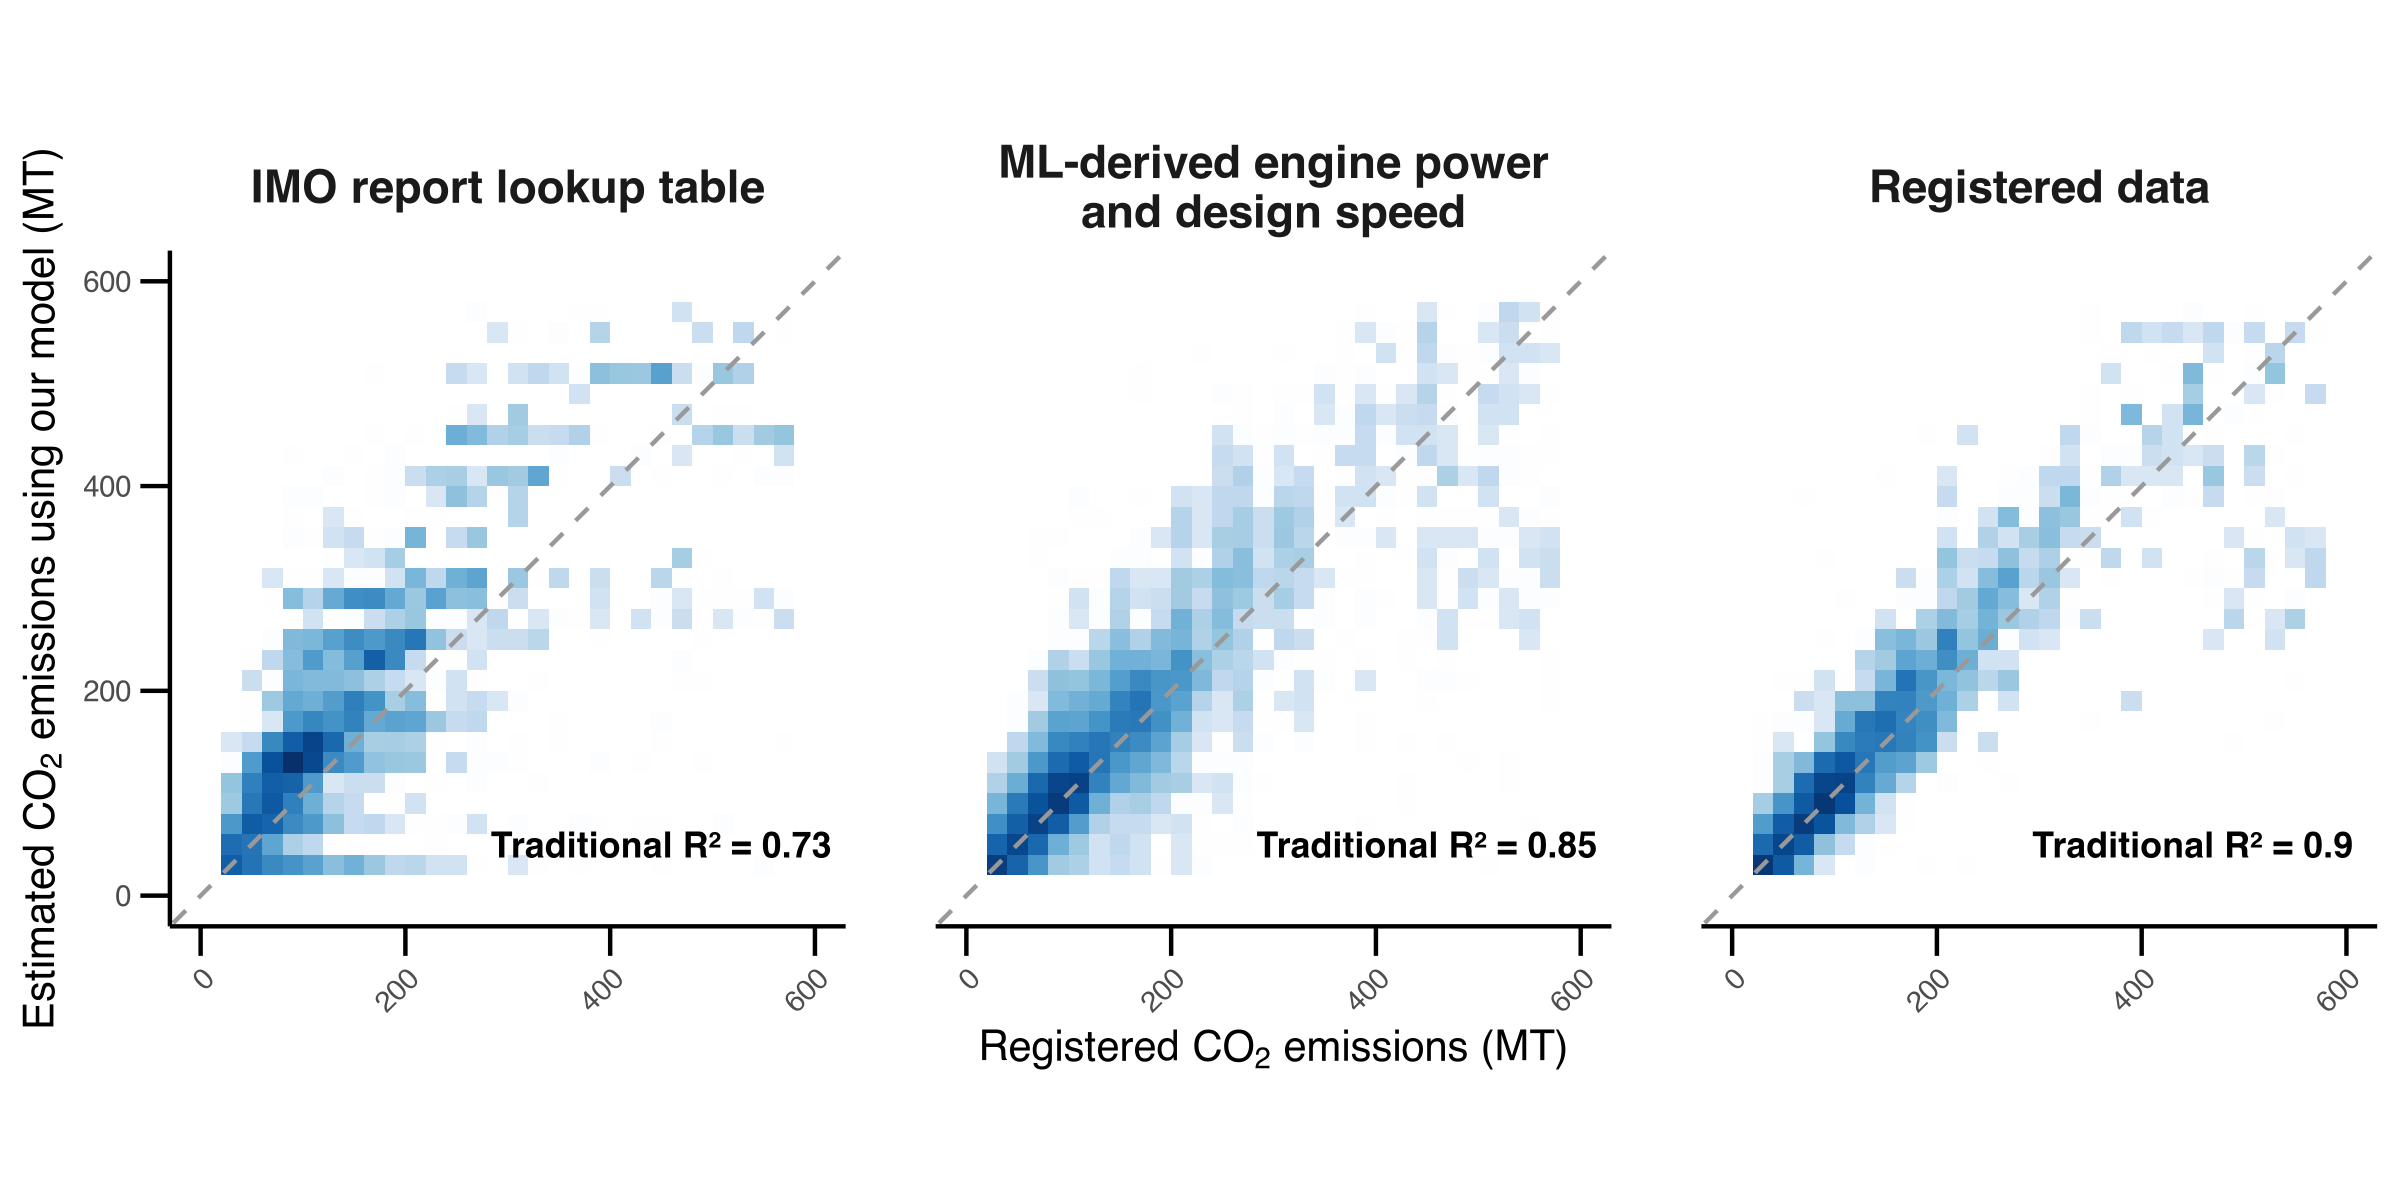
\includegraphics[width=\columnwidth]{figures/fig-registered-data-performance-1.png}
    \caption{Comparison of daily vessel-level CO$_{2}$ emissions estimated using our model with registered emissions from a proprietary vessel database (\DIFaddbeginFL \DIFaddFL{S\&P Global Market Intelligence's Ships Dataset; }\DIFaddendFL based on main engine fuel consumption over 24 hours). Estimates are shown using main engine power and design speed from IMO (left), our machine learning random forest models (center), and the same registered dataset (right). The \DIFdelbeginFL \DIFdelFL{solid red line shows a linear regression fit, while the }\DIFdelendFL dashed line represents the 1:1 line. Performance values for traditional R$^{2}$ are shown for each set of vessel characteristics. Over \DIFdelbeginFL \DIFdelFL{15}\DIFdelendFL \DIFaddbeginFL \DIFaddFL{16}\DIFaddendFL ,000 vessels are represented in the figure, and blue shading indicates point density. All data are rule-of-three compliant, meaning each cell (20×20 mt) displayed contains at least three vessels.}
    \label{fig:fig-registered-data-performance}
\end{figure}

\paragraph{EU MRV data validation}

We also validate our CO$_{2}$ emissions model results against public emissions data from the European Maritime Safety Agency’s Monitoring, Reporting, and Verification (MRV) program  \cite{mrv_emissions}. The MRV dataset provides yearly aggregated emissions—including CO$_{2}$ from main engines, auxiliary engines, gas turbines, boilers, and inert gas generators—along with hours at sea, and distance traveled for each vessel, covering voyages within, from, or to European Economic Area (EEA) “ports of call,” during which cargo is loaded/unloaded or passengers embark/disembark. It excludes port calls for refueling, supplies, crew changes, and similar activities.

Our AIS-derived emissions dataset does not contain detailed information on vessel activity while in port (i.e., whether or not cargo is loaded/unloaded or passengers embark/disembark), making it difficult to determine the exact same trip start and end points as defined in the MRV data, as well as which trips are included in the MRV records for a given year and vessel. To align vessel yearly activity across datasets, we: (1) filter our trip-level emissions data to include only trips that begin and/or end in EEA countries; (2) aggregate these trip-level emissions to annual emissions for each vessel; (3) apply varying matching tolerance margins to the MRV-reported annual hours at sea and select \DIFdelbegin \DIFdel{vessels-year }\DIFdelend \DIFaddbegin \DIFadd{vessel-years }\DIFaddend from our dataset within these limits, in order to ensure that the trips we use for comparison have a total hours at sea roughly equal to that reported in the MRV dataset; and (4) compare annual MRV emissions with the annual sum of our trip-level emissions for the same vessel and year to evaluate model performance.

\begin{table}[!h]
\centering
\caption{\label{tab:tab-performance-tolerance-table}Performance summary across different thresholds for the hours at sea tolerance between datasets. Results are shown using the R$^{2}$ (measuring linear association between observed and predicted values) and traditional R$^{2}$ (proportion of variance explained compared to the mean-only baseline).}
\centering
\fontsize{8}{10}\selectfont
\DIFdelbeginFL %DIFDELCMD < \begin{tabular}[t]{r|l|r|r}
%DIFDELCMD < \hline
%DIFDELCMD < Tolerance & Number of vessels & R$^{2}$ & Traditional R$^{2}$\\
%DIFDELCMD < \hline
%DIFDELCMD < 0.05 & 926 & 0.80 & 0.79\\
%DIFDELCMD < \hline
%DIFDELCMD < 0.10 & 1,598 & 0.80 & 0.79\\
%DIFDELCMD < \hline
%DIFDELCMD < 0.15 & 2,276 & 0.81 & 0.80\\
%DIFDELCMD < \hline
%DIFDELCMD < 0.20 & 2,918 & 0.77 & 0.75\\
%DIFDELCMD < \hline
%DIFDELCMD < 0.25 & 3,619 & 0.76 & 0.73\\
%DIFDELCMD < \hline
%DIFDELCMD < 0.30 & 4,394 & 0.66 & 0.52\\
%DIFDELCMD < \hline
%DIFDELCMD < 0.35 & 5,287 & 0.67 & 0.48\\
%DIFDELCMD < \hline
%DIFDELCMD < 0.40 & 6,339 & 0.68 & 0.40\\
%DIFDELCMD < \hline
%DIFDELCMD < \end{tabular}
%DIFDELCMD < %%%
\DIFdelendFL \DIFaddbeginFL \begin{tabular}[t]{r|l|r|r}
\hline
Tolerance & Number of observations & R$^{2}$ & Traditional R$^{2}$\\
\hline
0.05 & 11,621 & 0.84 & 0.83\\
\hline
0.10 & 20,432 & 0.85 & 0.84\\
\hline
0.15 & 27,657 & 0.85 & 0.84\\
\hline
0.20 & 33,753 & 0.85 & 0.83\\
\hline
0.25 & 38,980 & 0.84 & 0.82\\
\hline
0.30 & 43,958 & 0.83 & 0.81\\
\hline
0.35 & 48,399 & 0.83 & 0.80\\
\hline
0.40 & 52,490 & 0.82 & 0.79\\
\hline
\end{tabular}
\DIFaddendFL \end{table}
\DIFaddbegin \FloatBarrier
\DIFaddend 

In Table \ref{tab:tab-performance-tolerance-table}, performance peaks at a traditional R$^{2}$ of \DIFdelbegin \DIFdel{0.81 }\DIFdelend \DIFaddbegin \DIFadd{0.84 }\DIFaddend for vessels whose times at sea in our dataset are within 15\% of the MRV-reported values (validation sample of \DIFdelbegin \DIFdel{2,276 }\DIFdelend \DIFaddbegin \DIFadd{27,657 }\DIFaddend vessel-year observations\DIFaddbegin \DIFadd{, shown in Fig. \ref{fig:fig-mrv-performance}}\DIFaddend ). Beyond this threshold, performance declines as discrepancies grow between our annual aggregated trip activity and that recorded in the MRV dataset.


\begin{figure}[H]
    \centering
    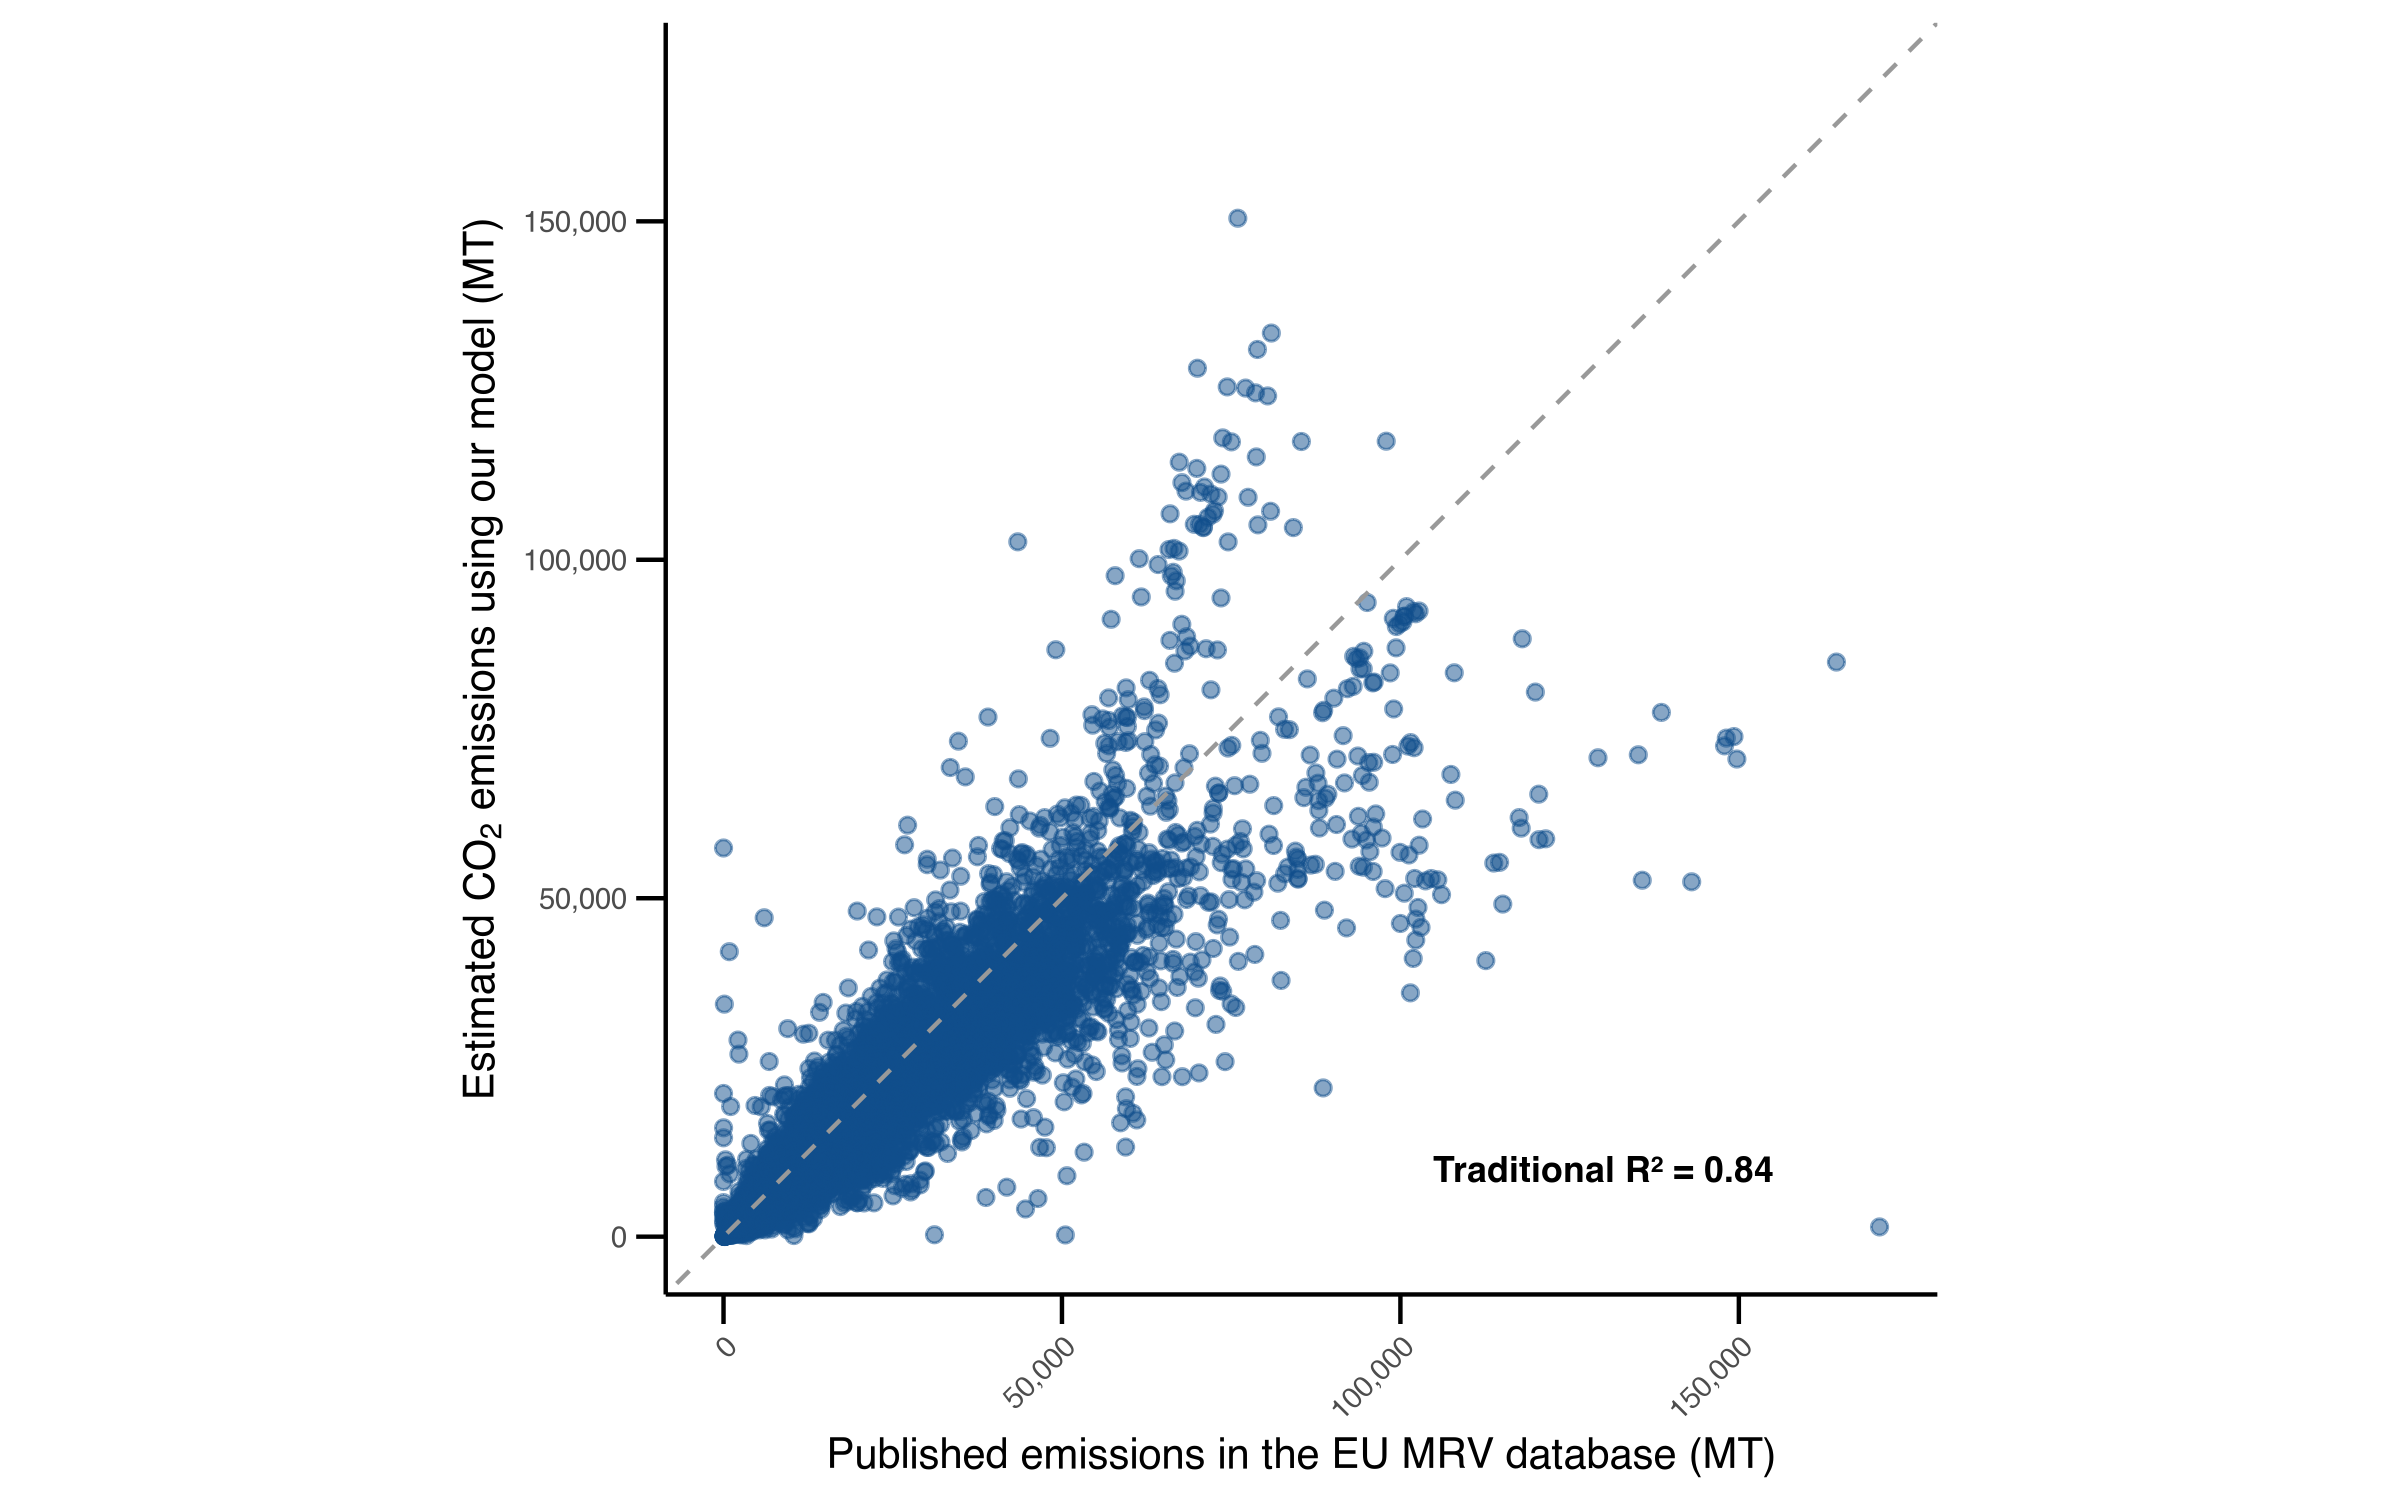
\includegraphics[width=\columnwidth]{figures/fig-mrv-performance-1.png}
    \caption{Comparison of annual vessel-level CO$_{2}$ emissions estimated using our model with published emissions from the EU MRV database. The sample includes \DIFdelbeginFL \DIFdelFL{2}\DIFdelendFL \DIFaddbeginFL \DIFaddFL{27}\DIFaddendFL ,\DIFdelbeginFL \DIFdelFL{276 }\DIFdelendFL \DIFaddbeginFL \DIFaddFL{657 }\DIFaddendFL observations from yearly aggregated vessel trips where hours at sea differ by no more than 15\% between our data and the MRV dataset. The \DIFdelbeginFL \DIFdelFL{solid red line shows the linear regression fit, and the }\DIFdelendFL dashed line represents the 1:1 line.}
    \label{fig:fig-mrv-performance}
\end{figure}

\subsection{\DIFdelbegin \DIFdel{Non-broadcasting vessels}\DIFdelend \DIFaddbegin \DIFadd{S1-unmatched vessel detections}\DIFaddend }\DIFaddbegin \label{sec:non-broadcasting-vessels}
\DIFaddend 

\subsubsection{Sentinel-1 SAR data description}

For our \DIFdelbegin \DIFdel{non-broadcasting vessel }\DIFdelend \DIFaddbegin \DIFadd{S1-unmatched }\DIFaddend emission estimates, we leverage GFW vessel detections from \DIFdelbegin \DIFdel{Sentinel-1 (}\DIFdelend S1 \DIFdelbegin \DIFdel{) }\DIFdelend Synthetic Aperture Radar (SAR) imagery \cite{paolo2024satellite}. \DIFdelbegin \DIFdel{For each vessel detection, the dataset provides its inferred vessel length and likelihood of being classified as either a fishing vessel or non-fishing vessel. By spatiotemporally matching AIS-broadcasting vessels to S1 detections, the dataset also categorizes each vessel detection as either an AIS-broadcasting vessel ('matched') or a non-broadcasting vessel ('unmatched') \mbox{%DIFAUXCMD
\cite{kroodsma2022revealing,paolo2024satellite}}\hskip0pt%DIFAUXCMD
. }\DIFdelend The data filtering involved in the GFW vessel detections include\DIFaddbegin \DIFadd{s}\DIFaddend  removing detections within a 1-km buffer from the shoreline to reduce false positives from land-based objects due to inaccurately defined and dynamic coastlines, repeated detections of potentially fixed objects such as offshore infrastructure, detections from icy areas, moving vehicles close to shore, and other radar ambiguities \cite{paolo2024satellite}. In addition, we also remove detections from known vessel anchorages \cite{gfw_anchorages_website}. \DIFaddbegin \DIFadd{Fishing gear is generally too small to be detected from Sentinel-1 SAR imagery, so no special filtering is needed to remove it from the dataset. }\DIFaddend Vessels detected at anchorage may or may not be active and actually emitting, so we \DIFdelbegin \DIFdel{limit our non-broadcasting vessel emissions estimation to focus only on those vessels that are away from anchorage and actively operating in the open water}\DIFdelend \DIFaddbegin \DIFadd{use only detections of vessels away from known anchorages as model inputs. Like the 1-km shoreline buffer, this filter restricts which detections enter our models, not which emissions are estimated: the emissions regression is trained on AIS-based emissions that also include activity in these areas, including emissions from vessels at berth (see below)}\DIFaddend . As a result, we used a dataset containing \DIFdelbegin \DIFdel{29.2 }\DIFdelend \DIFaddbegin \DIFadd{31.9 }\DIFaddend million vessel detections from 2017 to \DIFdelbegin \DIFdel{2024}\DIFdelend \DIFaddbegin \DIFadd{2025}\DIFaddend , of which \DIFdelbegin \DIFdel{13.5 }\DIFdelend \DIFaddbegin \DIFadd{14.9 }\DIFaddend million detections were not matched to \DIFdelbegin \DIFdel{a broadcasting vessel ('unmatched'}\DIFdelend \DIFaddbegin \DIFadd{an AIS-broadcasting vessel (referred to as `S1-unmatched'; the matching process is described in the next paragraph}\DIFaddend ). These detections come from across more than \DIFdelbegin \DIFdel{845}\DIFdelend \DIFaddbegin \DIFadd{924}\DIFaddend ,000 individual S1 scenes (\DIFdelbegin \DIFdel{(}\DIFdelend Fig. \ref{fig:fig-map-fraction-months-imaged}, Fig. \ref{fig:fig-s1-coverage-time-series}).

\DIFdelbegin \subsubsection{\DIFdel{Overview of non-broadcasting vessel emissions modeling framework}}
%DIFAUXCMD
\addtocounter{subsubsection}{-1}%DIFAUXCMD
\DIFdelend \DIFaddbegin \begin{figure}[H]
    \centering
    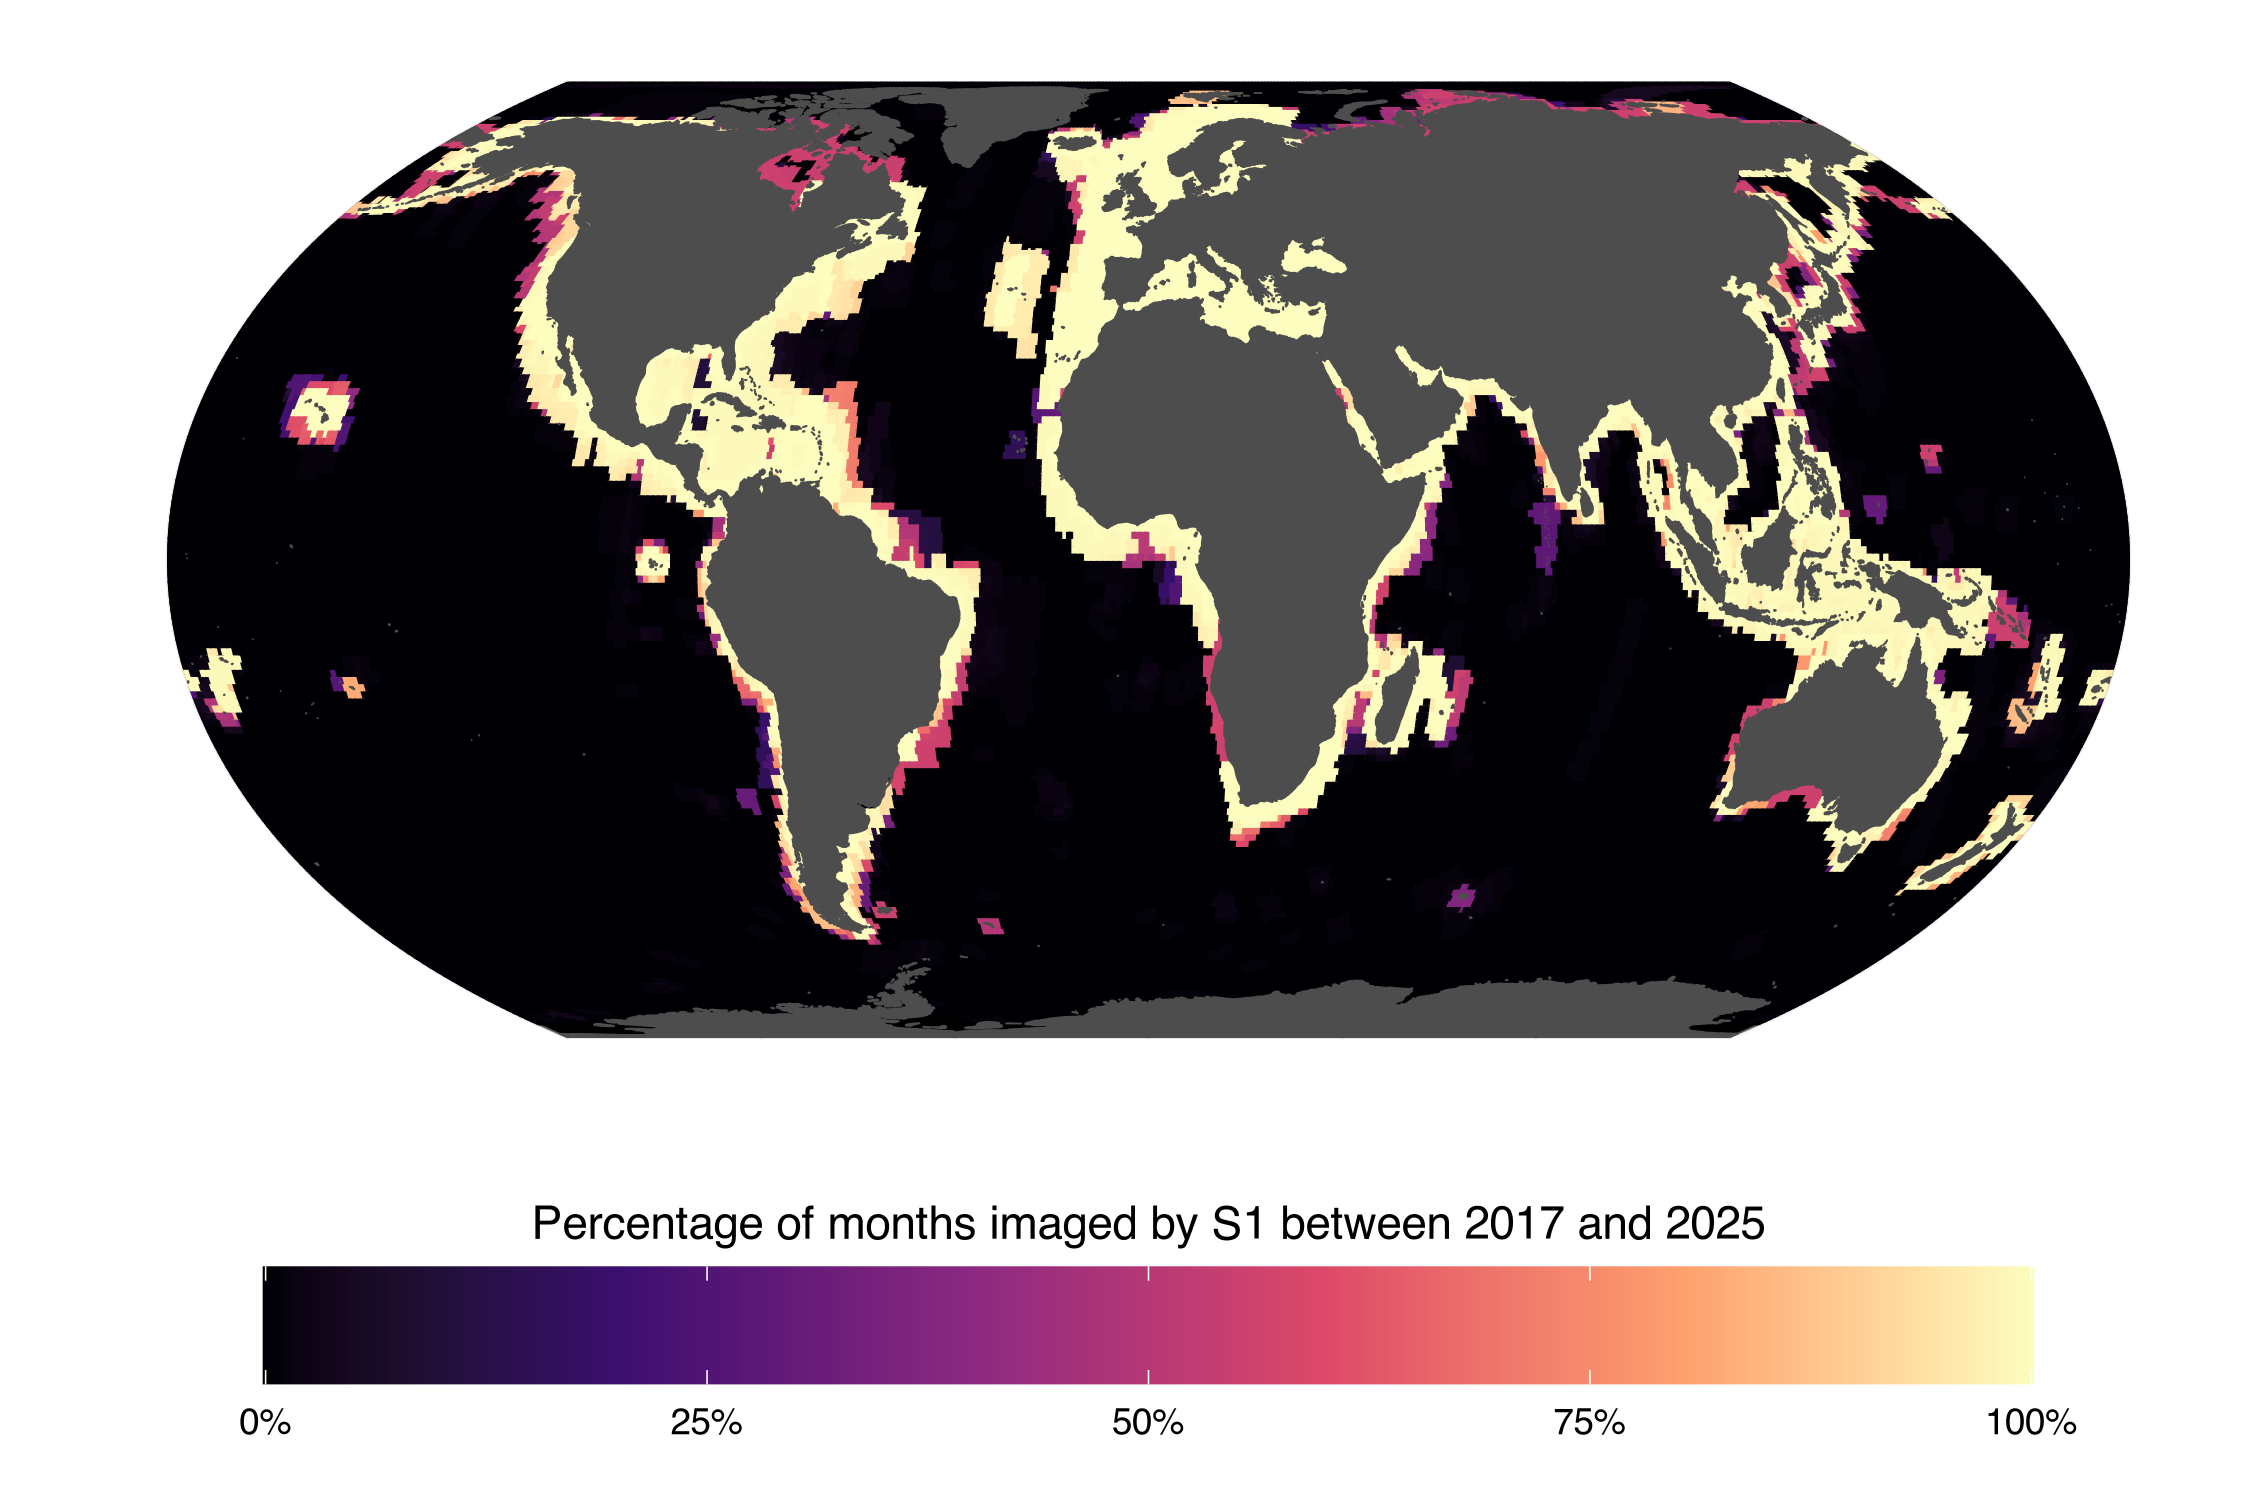
\includegraphics[width=\columnwidth]{figures/fig-map-fraction-months-imaged-1.png}
    \caption{\DIFaddFL{Map showing the percentage of months from 2017 through 2025 that were imaged by S1 for each 1x1 degree pixel.}}
    \label{fig:fig-map-fraction-months-imaged}
\end{figure}
\DIFaddend 


\DIFdelbegin \DIFdel{We estimate }\DIFdelend \DIFaddbegin \begin{figure}[H]
    \centering    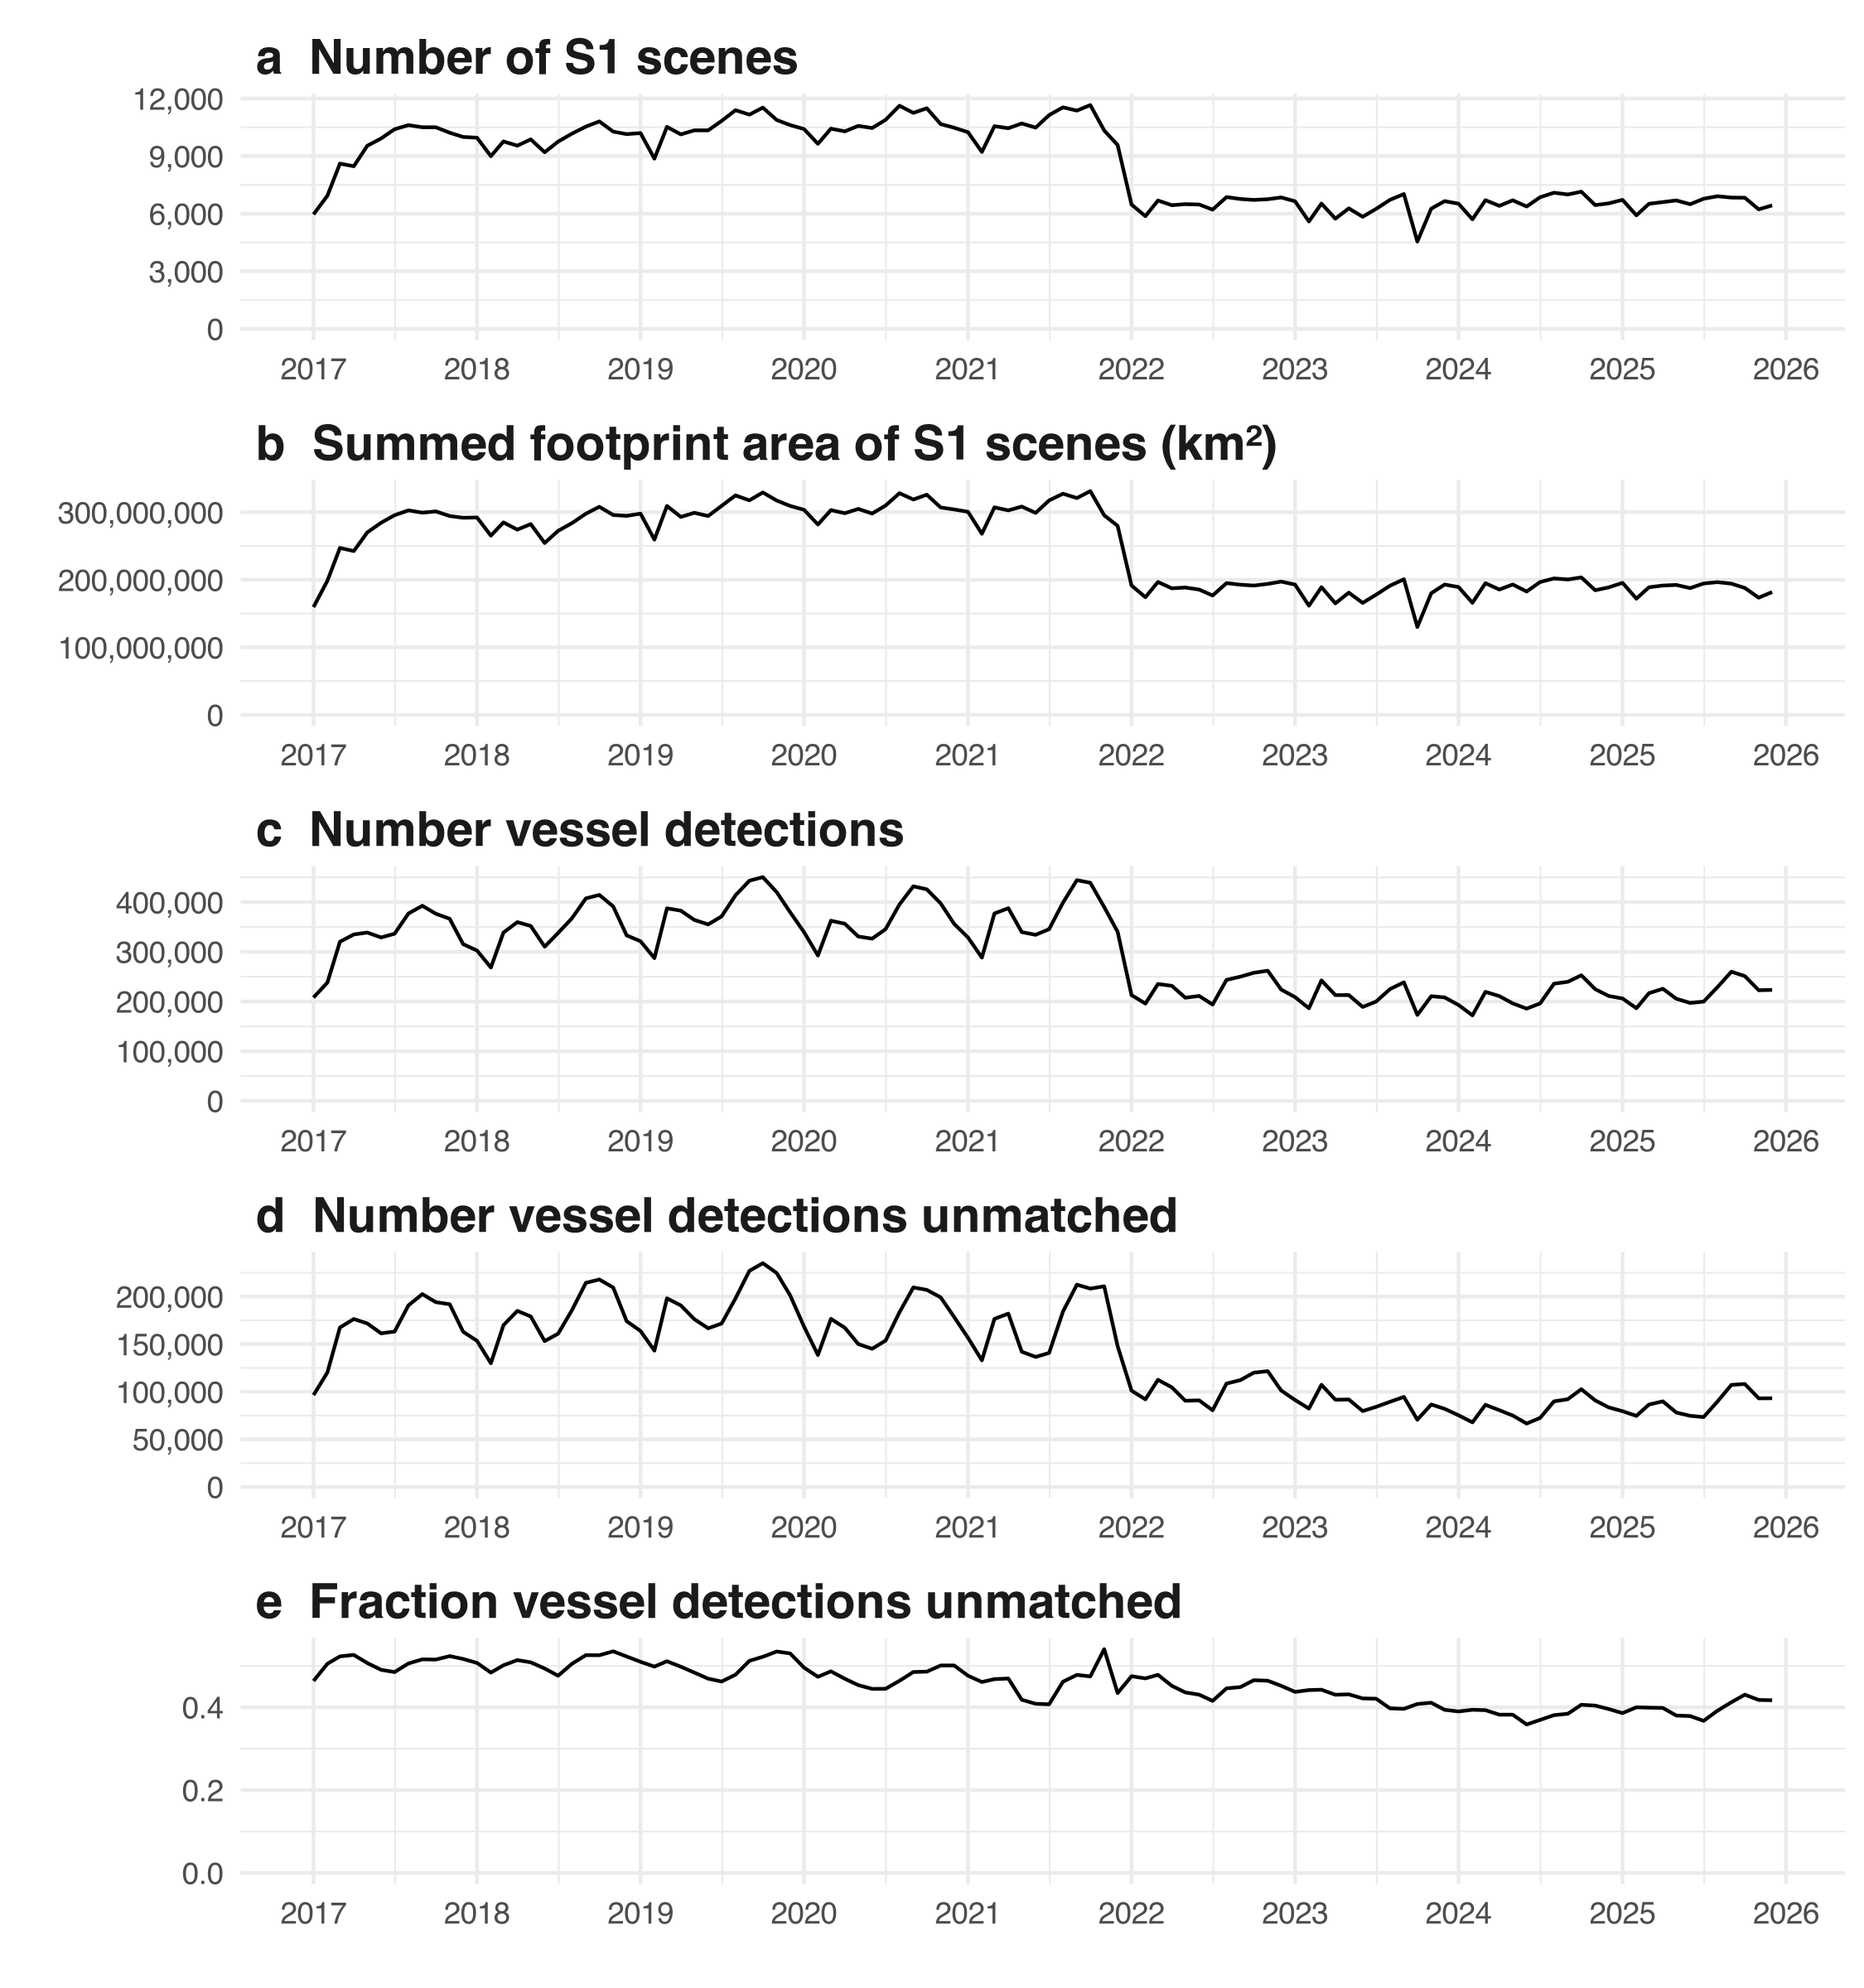
\includegraphics[width=\columnwidth]{figures/fig-s1-coverage-time-series-1.png}
    \caption{\DIFaddFL{Monthly statistics of global S1 coverage: (a) total number of S1 scenes; (b) total imaged area summed across all S1 scenes (which counts each revisit to a given area separately); (c) total number of vessel detections; (d) total number of vessel detections that could not be matched to an AIS-broadcasting vessel; and (e) fraction of vessel detections that could not be matched to an AIS-broadcasting vessel.}}
    \label{fig:fig-s1-coverage-time-series}
\end{figure}

\DIFadd{For each vessel detection, the dataset provides its inferred vessel length and likelihood of being classified as either a fishing vessel or non-fishing vessel. By spatiotemporally matching AIS-broadcasting vessels to S1 detections, the dataset also categorizes each vessel detection as either being matched to an AIS-broadcasting vessel (`matched'), or being unmatched to an AIS-broadcasting vessel (`unmatched') \mbox{%DIFAUXCMD
\cite{kroodsma2022revealing,paolo2024satellite}}\hskip0pt%DIFAUXCMD
. Importantly, although `unmatched' detections may often correspond to vessels that do not use AIS at all, it does not necessarily mean the vessel does not carry AIS - it could still carry AIS, but its transmission may be experiencing a gap for a variety of transmission or reception reasons. The detection-AIS matching utilizes a probabilistic framework that produces matching scores representing the likelihood of detection-AIS pairs being correct, and applies a global threshold to these scores \mbox{%DIFAUXCMD
\cite{kroodsma2022revealing,paolo2024satellite}}\hskip0pt%DIFAUXCMD
. The matching considers AIS positions before and after the detection timestamp up to 12 hours away, and larger AIS position gaps typically result in lower matching scores with candidate detections. Therefore, an unmatched detection in this study may correspond to either a vessel not equipped with AIS or a vessel equipped with AIS but experiencing a transmission gap. The transmission gap can be intentional or a result of poor AIS reception. A broadcasting vessel that goes unmatched in this way therefore erroneously has its emissions counted in both our `AIS-based' and `S1-unmatched' estimates, inflating our fused total. To estimate the extent of this double counting and its effect on our fused emissions estimates, we first use a hold-out experiment in which S1 detections with high-confidence AIS matches were re-matched using our matching algorithm but with AIS positions withheld within a window of the detection timestamp. This gives the probability that a detection of a broadcasting vessel is missed by the matching as a function of the AIS transmission gap; this rises gradually from 6.8\% at a 2-hour gap to 27.4\% at 8 hours and 45.4\% at 18 hours (Fig. \ref{fig:fig-s1-matching-double-counting}a). Second, because each AIS message represents the interval since the vessel's previous message, we know how much of our AIS-based CO$_{2}$ is emitted during gaps of each length (Fig. \ref{fig:fig-emissions-by-message-hour-threshold}, Fig. \ref{fig:fig-s1-matching-double-counting}b). Multiplying the two gives the share of AIS-based emissions emitted during gaps in which a detection of the vessel would have been missed, which we call the share at risk of double counting: 5.1\% (Fig. \ref{fig:fig-s1-matching-double-counting}c-d, Table \ref{tab:s1_matching_double_counting_by_gap}). Because S1 images a vessel at an arbitrary moment, this share is also the probability that any given detection of a broadcasting vessel is missed. Our 17.0 million matched detections are therefore the 94.9\% that were not missed, and the remaining 0.92 million detections of broadcasting vessels are among our 14.9 million unmatched detections, where they make up 6.2\% of the total. Our S1-unmatched emissions are estimated from the density of unmatched detections, so a missed broadcasting vessel contributes to them like any other unmatched detection, and about 6.2\% of S1-unmatched emissions (136 million tonnes over 2017 to 2025, or 1.2\% of our combined total) therefore duplicate emissions already included in our AIS-based estimate. Finally, the missed detections are also absent from the matched detections used to train the emissions regression model, which raises the emissions it assigns to each detection by 5.4\%. Up to 11.0\% of our S1-unmatched emissions may therefore be due to double counting from missed matches during AIS transmission gaps; this translates to 2.2\% of our total fused emissions (Table \ref{tab:s1_matching_double_counting_summary}). 
}

\begin{figure}[H]
    \centering
    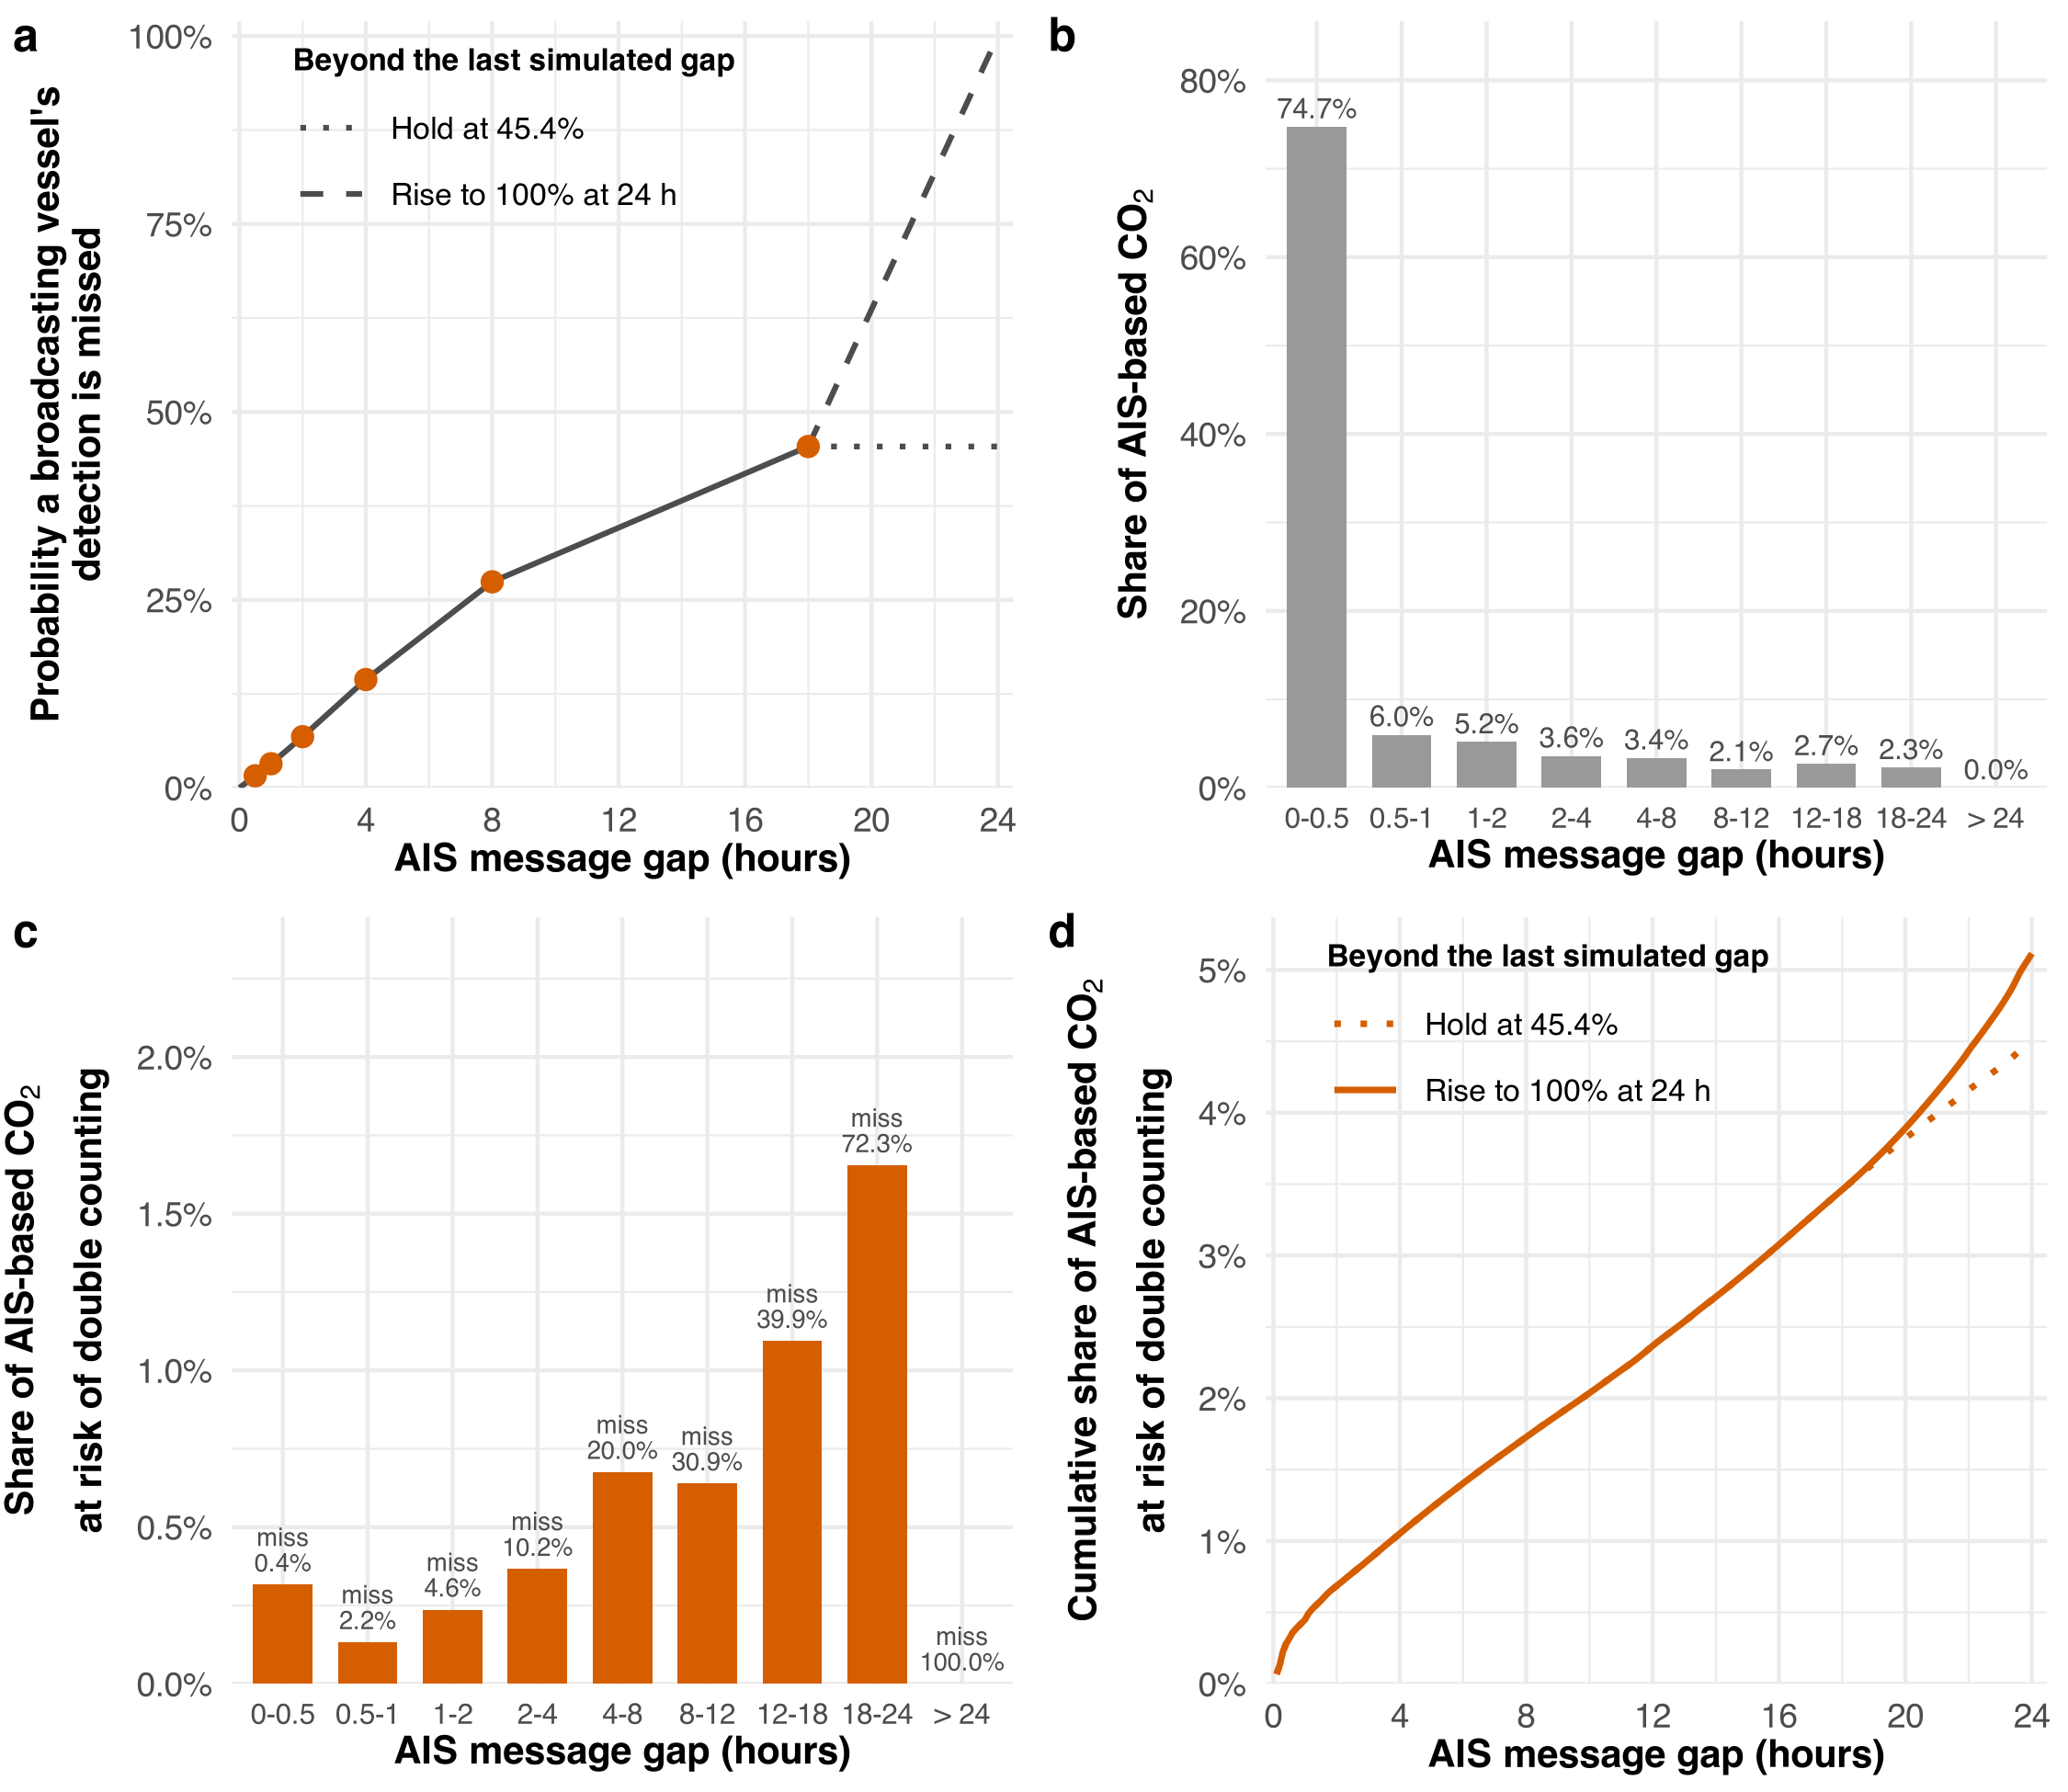
\includegraphics[width=\columnwidth]{figures/fig-s1-matching-double-counting-1.png}
    \caption{\DIFaddFL{(a) Probability that a detection of an AIS-broadcasting vessel is missed by the matching, by the length of the gap in its AIS messages. Beyond the last simulated gap, we assume the line either reaches 100\% at the 24-hour matching window (dashed) or stays flat (dotted). (b) Share of AIS-based CO$_{2}$ emissions, 2017 to 2025, by the length of the AIS gap during which they were emitted. (c) Panel b multiplied by panel a, the share of AIS-based emissions at risk of double counting: emitted during gaps in which a detection of the vessel would have been missed and counted as S1-unmatched. The miss probability for each bin is labeled above the bar. (d) Cumulative total of panel c; the end point is the 5.1\% in the text.}}
    \label{fig:fig-s1-matching-double-counting}
\end{figure}

\begin{table}[!h]
\centering
\caption{\label{tab:s1_matching_double_counting_by_gap}\DIFaddFL{AIS-based CO$_2$ emissions by the length of the AIS gap during which they were emitted, 2017 to 2025, and the share at risk of double counting: the emissions in each row multiplied by the probability that an S1 detection made during a gap of that length is missed by the matching (Fig. \ref{fig:fig-s1-matching-double-counting}a). Beyond 18 hours the miss rate is taken to reach 100\% at 24 hours; messages representing more than 24 hours are treated as always missed.}}
\centering
\fontsize{8}{10}\selectfont
\begin{tabular}[t]{lrrrr}
\toprule
Gap (hours) & Share of CO$_2$ & Miss rate & At risk & Cumulative at risk\\
\midrule
0-0.5 & 74.73\% & 0.4\% & 0.32\% & 0.32\%\\
0.5-1 & 6.00\% & 2.2\% & 0.13\% & 0.45\%\\
1-2 & 5.19\% & 4.6\% & 0.24\% & 0.69\%\\
2-4 & 3.61\% & 10.2\% & 0.37\% & 1.05\%\\
4-8 & 3.37\% & 20.0\% & 0.68\% & 1.73\%\\
\addlinespace
8-12 & 2.07\% & 30.9\% & 0.64\% & 2.37\%\\
12-18 & 2.74\% & 39.9\% & 1.09\% & 3.46\%\\
18-24 & 2.29\% & 72.3\% & 1.65\% & 5.12\%\\
$>$ 24 & 0.00\% & 100.0\% & 0.00\% & 5.12\%\\
\bottomrule
\end{tabular}
\end{table}
\begin{table}[!h]
\centering
\caption{\label{tab:s1_matching_double_counting_summary}\DIFaddFL{Double counting between the AIS-based and S1-unmatched CO$_2$ estimates, 2017 to 2025, following the steps in the text. The share at risk is the total of Table \ref{tab:s1_matching_double_counting_by_gap}; because S1 images a vessel at an arbitrary moment, it is also the probability that a detection of a broadcasting vessel is missed by the matching. The matched detections are the ones that were not missed, which gives the number missed and their share of the unmatched detections. S1-unmatched emissions are estimated from unmatched detections, so that share of them duplicates AIS-based emissions. The last two rows add the effect of the missed detections being absent from the matched detections the emissions regression model is trained on. The miss rate beyond 18 hours is taken to reach 100\% at 24 hours (Fig. \ref{fig:fig-s1-matching-double-counting}a, dashed).}}
\centering
\fontsize{8}{10}\selectfont
\begin{tabular}[t]{>{\raggedright\arraybackslash}p{7cm}>{\raggedleft\arraybackslash}p{4cm}}
\toprule
  & Value\\
\midrule
Share of AIS-based CO$_2$ at risk of double counting & 5.1\%\\
Matched S1 detections & 17.0 million\\
Detections of broadcasting vessels missed by the matching & 0.92 million\\
Unmatched S1 detections & 14.9 million\\
Share of unmatched detections that are broadcasting vessels & 6.2\%\\
\addlinespace
S1-unmatched CO$_2$ that duplicates AIS-based CO$_2$, 2017--2025 & 136 million tonnes (1.2\% of combined total)\\
Increase in the emissions the model fits per detection & 5.4\%\\
Upper bound on S1-unmatched CO$_2$ that duplicates AIS-based CO$_2$, including that increase & 11.0\% of S1-unmatched CO$_2$ (2.2\% of combined total)\\
\bottomrule
\end{tabular}
\end{table}
\FloatBarrier

\subsubsection{\DIFadd{Overview of S1-unmatched emissions modeling framework}}

\DIFadd{Here we describe our model for estimating S1-unmatched emissions at a 1x1-degree gridded resolution with global coverage, consistently each month from 2017 through 2025, and disaggregated by vessel type (fishing or non-fishing). A common limitation in SAR-derived inventories is the sparse temporal coverage of Low Earth Orbit satellites, where dynamic vessel movements are inadequately captured by discrete, fixed-time overpasses. To address this spatiotemporal mismatch, we avoid assuming steady-state vessel activity from snapshots of imagery. Instead, we estimate S1-unmatched }\DIFaddend emissions \DIFdelbegin \DIFdel{from non-broadcasting vessels }\DIFdelend using a multi-model framework that uses a combination of AIS-derived emissions, S1 vessel detections, and additional spatiotemporal model features \DIFdelbegin \DIFdel{. Let's }\DIFdelend \DIFaddbegin \DIFadd{based on an observational unit of 1x1 degree pixel-months. Because S1 detections are anonymous snapshots, we do not reconstruct vessel trajectories from them. Our models learn from AIS-broadcasting vessels how the density of detections in these snapshots relates to total monthly emissions in each pixel. S1 follows a sun-synchronous dawn-dusk orbit, so it images each location at nearly the same local times on every pass, and applying this relationship to unmatched detections assumes that unmatched vessels follow daily activity patterns similar to those of matched vessels in the same pixel-month. Our out-of-sample tests measure how well this approach recovers monthly emissions from snapshots (Table \ref{tab:all_performance_metrics_table}). We }\DIFaddend first consider the case of modeling \DIFdelbegin \DIFdel{non-broadcasting }\DIFdelend \DIFaddbegin \DIFadd{S1-unmatched }\DIFaddend CO$_2$ emissions. For the first model, we build a regression random forest to predict \DIFdelbegin \DIFdel{AIS-broadcasting }\DIFdelend \DIFaddbegin \DIFadd{AIS-based }\DIFaddend CO$_2$ emissions using matched S1 detection \DIFdelbegin \DIFdel{detection }\DIFdelend density and additional spatiotemporal model features (subsequently referred to as the \DIFdelbegin \DIFdel{'}\DIFdelend \DIFaddbegin \DIFadd{`}\DIFaddend emissions regression' model). We can then use this model to predict \DIFdelbegin \DIFdel{non-broadcasting }\DIFdelend \DIFaddbegin \DIFadd{S1-unmatched }\DIFaddend CO$_2$ emissions using unmatched S1 detection density (i.e., detections \DIFdelbegin \DIFdel{from non-broadcasting vessels}\DIFdelend \DIFaddbegin \DIFadd{not matched to an AIS-broadcasting vessel}\DIFaddend ). Because this model requires data for both \DIFdelbegin \DIFdel{AIS-broadcasting }\DIFdelend \DIFaddbegin \DIFadd{AIS-based }\DIFaddend emissions and S1 detections, it is trained using data from pixel-month observations that are imaged by S1 (Fig. \ref{fig:fig-map-fraction-months-imaged}). For pixel-month observations that are imaged by S1, we can use the directly observed unmatched S1 detection density for this prediction. 

Not all pixel-month observations are \DIFdelbegin \DIFdel{not }\DIFdelend imaged by S1, either because there were simply no S1 overpasses in a given area and month, or because a given area is completely outside the S1 footprint (Fig. \ref{fig:fig-map-fraction-months-imaged}). For these observations without S1 imaging, we interpolate unmatched detection density using a two-stage hurdle framework which is composed of two models: (1) a classification random forest that predicts the presence or absence of unmatched detections (subsequently referred to as the \DIFdelbegin \DIFdel{'}\DIFdelend \DIFaddbegin \DIFadd{`}\DIFaddend detection classification' model); and (2) a regression random forest \DIFdelbegin \DIFdel{regression }\DIFdelend to estimate the density of unmatched detections, conditional on there being any detections present  (subsequently referred to as the \DIFdelbegin \DIFdel{'}\DIFdelend \DIFaddbegin \DIFadd{`}\DIFaddend detection regression' model). Therefore, for pixel-months not imaged by S1, we can use the predicted density of unmatched detections from the \DIFdelbegin \DIFdel{'}\DIFdelend \DIFaddbegin \DIFadd{`}\DIFaddend detection regression' model as an input to the \DIFdelbegin \DIFdel{'}\DIFdelend \DIFaddbegin \DIFadd{`}\DIFaddend emissions regression' model in order to predict the amount of \DIFdelbegin \DIFdel{non-broadcasting }\DIFdelend \DIFaddbegin \DIFadd{S1-unmatched }\DIFaddend CO$_2$ emissions in these areas.


\DIFdelbegin %DIFDELCMD < \begin{figure}[H]
%DIFDELCMD <     \centering
%DIFDELCMD <     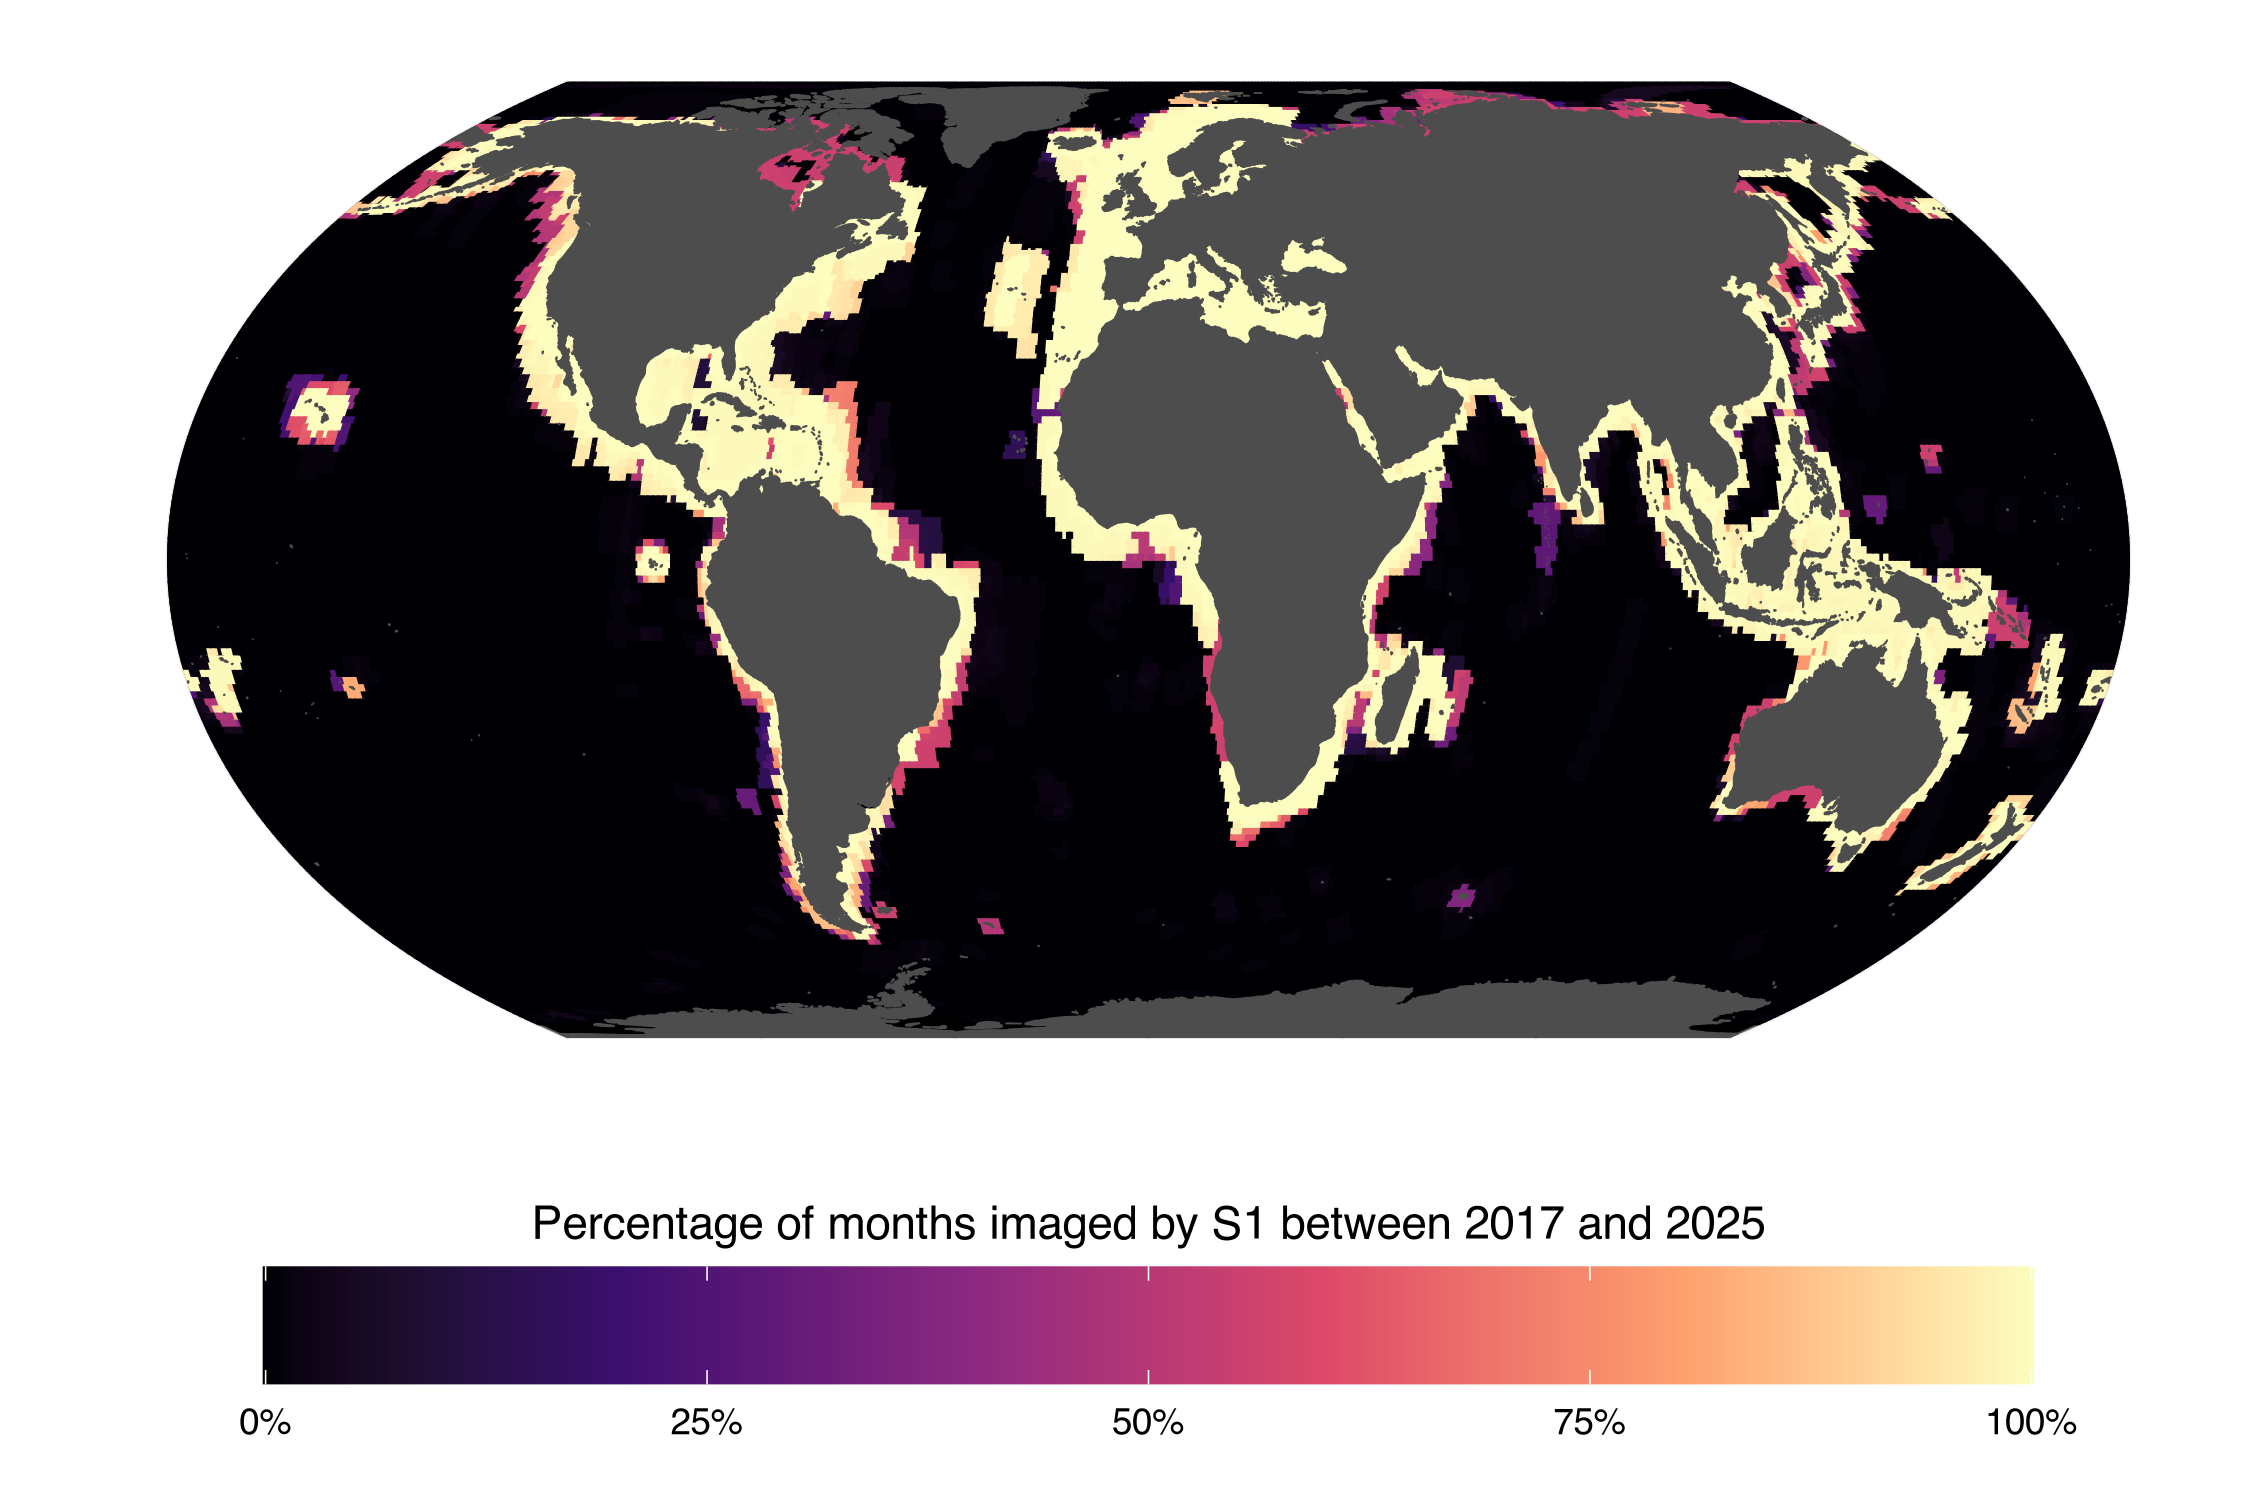
\includegraphics[width=\columnwidth]{figures/fig-map-fraction-months-imaged-1.png}
%DIFDELCMD <     %%%
%DIFDELCMD < \caption{%
{%DIFAUXCMD
\DIFdelFL{Map showing the percentage of months from 2017 through 2024 that were imaged by S1 for each 1x1 degree pixel.}}
    %DIFAUXCMD
%DIFDELCMD < \label{fig:fig-map-fraction-months-imaged}
%DIFDELCMD < \end{figure}
%DIFDELCMD < 

%DIFDELCMD < %%%
\DIFdelend To reduce overall model complexity, we use a more simplified approach for estimating \DIFdelbegin \DIFdel{non-broadcasting }\DIFdelend \DIFaddbegin \DIFadd{S1-unmatched }\DIFaddend emissions for the other eight gases (the other two GHGs and six pollutants). With our AIS-based emissions model, emissions of all gases are calculated using gas-specific emissions factors that linearly convert \DIFaddbegin \DIFadd{either fuel consumption or }\DIFaddend engine energy use (kil\DIFdelbegin \DIFdel{l}\DIFdelend owatt-hours ) to emissions \DIFaddbegin \DIFadd{(with energy use being closely correlated to fuel consumption)}\DIFaddend . Emissions of all non-CO$_2$ gases are therefore highly correlated with CO$_2$ emissions (although there are some non-linearities: \DIFaddbegin \DIFadd{for example, }\DIFaddend different vessel types and sizes have different emissions factors for \DIFdelbegin \DIFdel{auxillary }\DIFdelend \DIFaddbegin \DIFadd{auxiliary }\DIFaddend engine and boiler energy use; we apply correction factors for some pollutants when engines are operating at very low loads; the 2020 IMO low \DIFdelbegin \DIFdel{sulphur }\DIFdelend \DIFaddbegin \DIFadd{sulfur }\DIFaddend policy affects emissions factors of some pollutants but not others). Therefore, rather than training nine separate random forest models to predict emissions for each of the nine gases, we simplify the overall modeling framework by building a single random forest to predict CO$_2$ emissions and then eight linear regression models to predict emissions of each gas from the emissions of CO$_2$. \DIFaddbegin \DIFadd{Each of these linear models is composed of five coefficients. }\DIFaddend To account for the temporal discontinuity that occurs when the 2020 IMO low \DIFdelbegin \DIFdel{sulphur }\DIFdelend \DIFaddbegin \DIFadd{sulfur }\DIFaddend policy was implemented, we include \DIFdelbegin \DIFdel{an interaction term with }\DIFdelend a post-2020 dummy variable\DIFdelbegin \DIFdel{and CO$_2$ emissions }\DIFdelend \DIFaddbegin \DIFadd{. To account for the fact that fishing and non-fishing vessels have slightly different emissions profiles, we interact the post-2020 dummy variable with a dummy variable for fishing/non-fishing  }\DIFaddend such that regression coefficients are estimated separately for pre- and post-2020 periods \DIFaddbegin \DIFadd{for both fishing and non-fishing vessels (yielding four separate coefficients). Finally, to account for the fact that there are spatial patterns in terms of where vessels of different sizes are located, and that different size vessels have different emissions profiles, we include a coefficient for $\log(\text{distance to shore} + 1)$}\DIFaddend . 

\DIFdelbegin \DIFdel{$emissions_{gas,i} = \beta_1 *emissions_{CO2,i} * {post2020_{FALSE}}  + \beta_2 * emissions_{CO2,i} * {post2020_{TRUE}} + \epsilon_i$
}\DIFdelend \DIFaddbegin \begin{align*}
\DIFadd{\text{emissions}_{\text{gas},i} = }{} 
  & \DIFadd{\beta_1 \times \text{emissions}_{\text{CO}_2,i} \times \text{post2020}_{\text{FALSE}} \times \text{fishing}_{\text{FALSE}} }\\
  & \DIFadd{+ \beta_2 \times \text{emissions}_{\text{CO}_2,i} \times \text{post2020}_{\text{TRUE}} \times \text{fishing}_{\text{FALSE}} }\\
  & \DIFadd{+ \beta_3 \times \text{emissions}_{\text{CO}_2,i} \times \text{post2020}_{\text{FALSE}} \times \text{fishing}_{\text{TRUE}} }\\
  & \DIFadd{+ \beta_4 \times \text{emissions}_{\text{CO}_2,i} \times \text{post2020}_{\text{TRUE}} \times \text{fishing}_{\text{TRUE}} }\\
  & \DIFadd{+ \beta_5 \times \text{emissions}_{\text{CO}_2,i} \times \log(\text{distance\_to\_shore} + 1) + \epsilon_i
}\end{align*}
\DIFaddend 

Therefore, for all non-CO$_2$ gases, we first predict \DIFdelbegin \DIFdel{non-broadcasting }\DIFdelend \DIFaddbegin \DIFadd{S1-unmatched }\DIFaddend CO$_2$ emissions using the framework above, and then convert these emissions to non-CO$_2$ \DIFdelbegin \DIFdel{non-broadcasting }\DIFdelend \DIFaddbegin \DIFadd{S1-unmatched }\DIFaddend emissions using these eight linear models. \DIFaddbegin \DIFadd{Pollutant-to-CO$_2$ ratios were evaluated with distance to shore winsorized at the 0.1st percentile of the fitting distribution (442 m), to avoid extrapolating the log-linear ratio below the support of the data, where it can become negative.
}\DIFaddend 

In the sections below, we detail: 1) the unit of observation and outcome variable for each of the three models; 2) the features used in each of the three models; 3) the data pre-processing steps used for each model; 4) the performance testing procedures and results for each model; 5) the feature importance results for each model; and 6) the final prediction procedure for obtaining our global spatiotemporal \DIFdelbegin \DIFdel{non-broadcasting vessel }\DIFdelend \DIFaddbegin \DIFadd{S1-unmatched }\DIFaddend emissions estimates.

\subsubsection{Units of observation and outcome variables}

\paragraph{Emissions regression} The observation unit for predicting emissions is the total emissions (of a given GHG or pollutant) in a given 1x1 degree ocean pixel, in a given month, for a given type of vessel (either non-fishing or fishing). For model training, we used the emissions estimated from the \DIFdelbegin \DIFdel{AIS-broadcasting }\DIFdelend \DIFaddbegin \DIFadd{AIS-based }\DIFaddend model, extracting ping-level emissions from broadcasting vessels that occurred in \DIFdelbegin \DIFdel{ocean water beyond }\DIFdelend \DIFaddbegin \DIFadd{marine waters (the ocean and coastal cells of }\DIFaddend a 1\DIFdelbegin \DIFdel{km buffer from shore, which corresponds to the spatial coverage of S1 detections processed by GFW and therefore }\DIFdelend \DIFaddbegin \DIFadd{/20-degree land--water classification), which }\DIFaddend excludes inland waterways, lakes, rivers, and \DIFdelbegin \DIFdel{ports}\DIFdelend \DIFaddbegin \DIFadd{canals. Unlike the S1 detections, these emissions are not subject to the 1-km shoreline buffer or the anchorage filter, and they include emissions from vessels at berth in coastal ports, so the model learns the relationship between the detections S1 can observe and total emissions in each pixel}\DIFaddend . These ping-level emissions were aggregated to our unit of observation (by 1x1 degree pixel, month, and fishing/non-fishing vessel types), and observations with zero \DIFdelbegin \DIFdel{AIS-broadcasting emissions }\DIFdelend \DIFaddbegin \DIFadd{AIS-based emissions or no matched S1 detections }\DIFaddend were excluded. Emissions for each observation are aggregated across all vessel sizes. 

For the random forest to predict CO$_2$ emissions, in order to capture the vessel length distribution of S1 detections across different vessel sizes, for each observation we include several model features that represent the number of S1 detections in each of several vessel length bins. For non-fishing vessels, we use 10 length bins: 0-25m, 25-50m, ..., 200-225m, and 225+ m;  for fishing vessels, which are typically smaller, we use five length bins: 0-25m, 25-50m, 50-75m, 75-100m, and 100+ m (Fig. \ref{fig:fig-length-bin-distributions}). We use length bins because length is representative of main engine power (Fig. \ref{fig:fig-ais-length-power-relationship}), which is directly related to emissions in our AIS-based model. We stratify by vessel type (fishing or non-fishing) because they have significantly different length size distributions (Fig. \ref{fig:fig-length-bin-distributions}), and also because some fishing vessel types have fundamentally different emissions profiles than non-fishing vessels (i.e., trawlers and dredgers emit more at low speeds due to the nature of their energy-intensive gear deployment, which is reflected in their gear-specific main engine load factor adjustment.) Additionally, because emissions are highly right-skewed, we log-normalize the CO$_2$ emissions as the dependent variable. 

\begin{figure}[H]
    \centering
    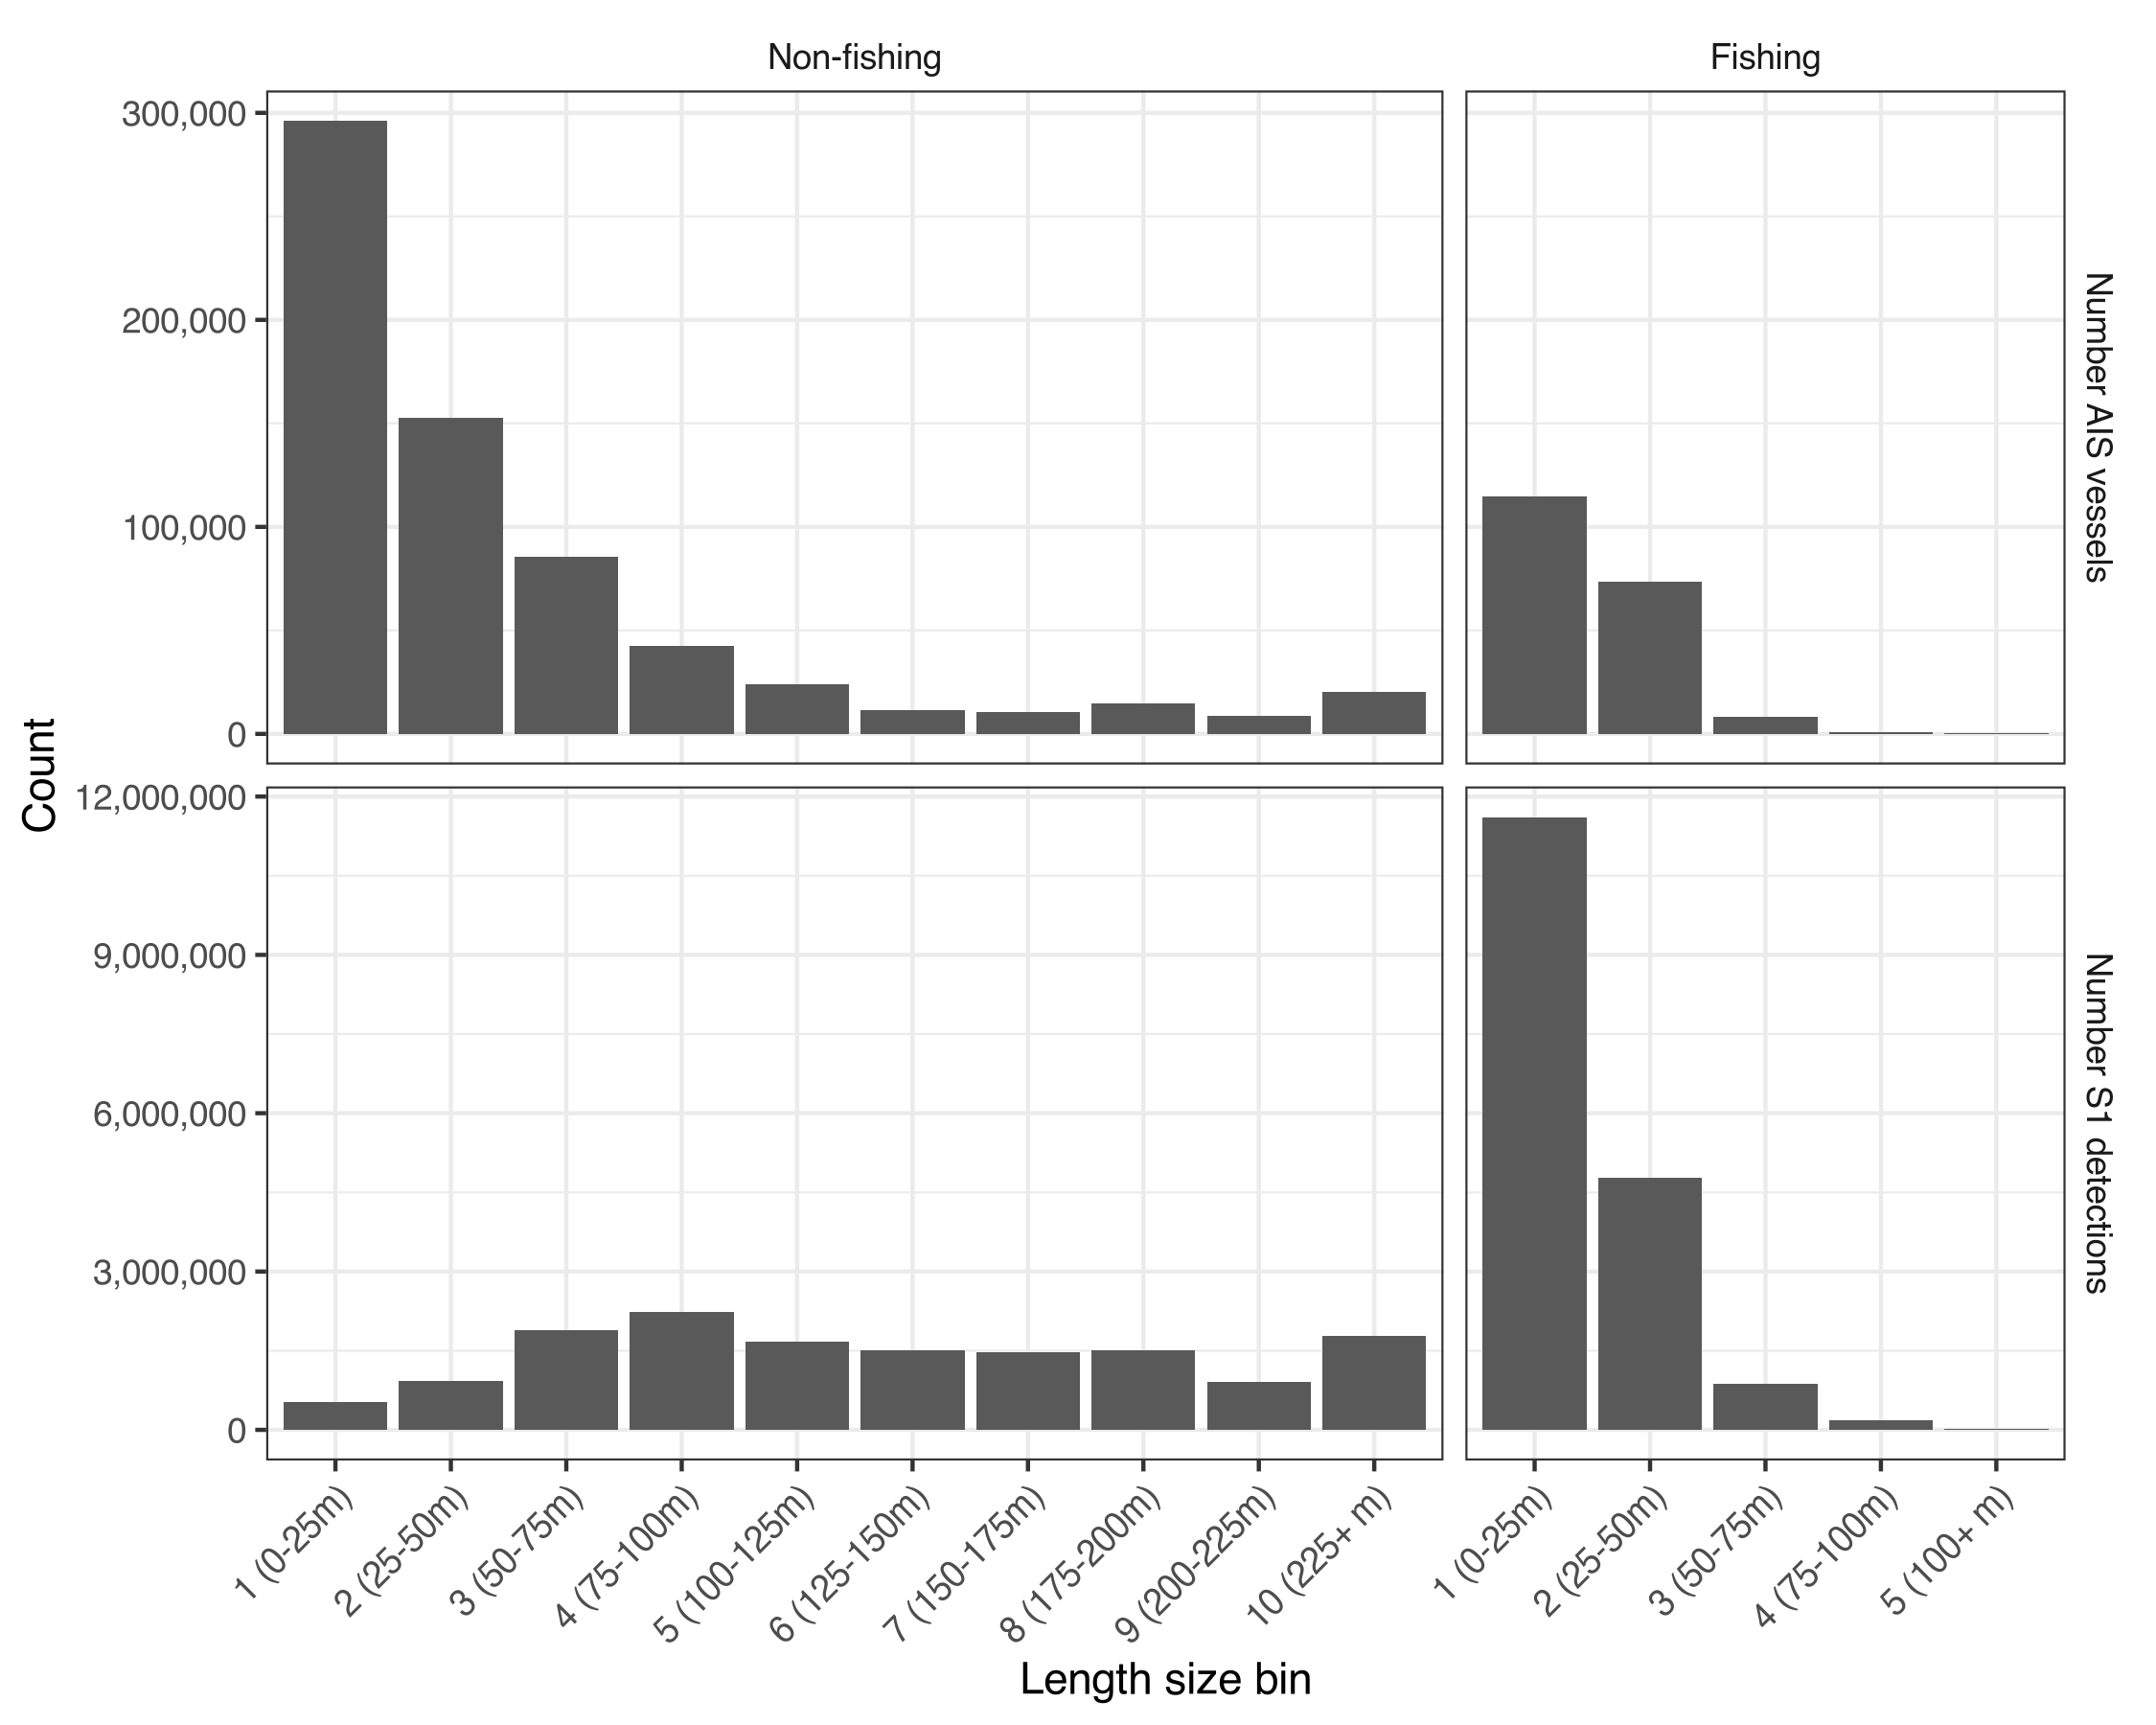
\includegraphics[width=\columnwidth]{figures/fig-length-bin-distributions-1.png}
    \caption{Distributions showing the number of unique AIS vessels and number of S1 detections for each length size bin, \DIFdelbeginFL \DIFdelFL{disaggregted }\DIFdelendFL \DIFaddbeginFL \DIFaddFL{disaggregated }\DIFaddendFL by non-fishing and fishing vessels.}
    \label{fig:fig-length-bin-distributions}
\end{figure}

\begin{figure}[H]
    \centering
    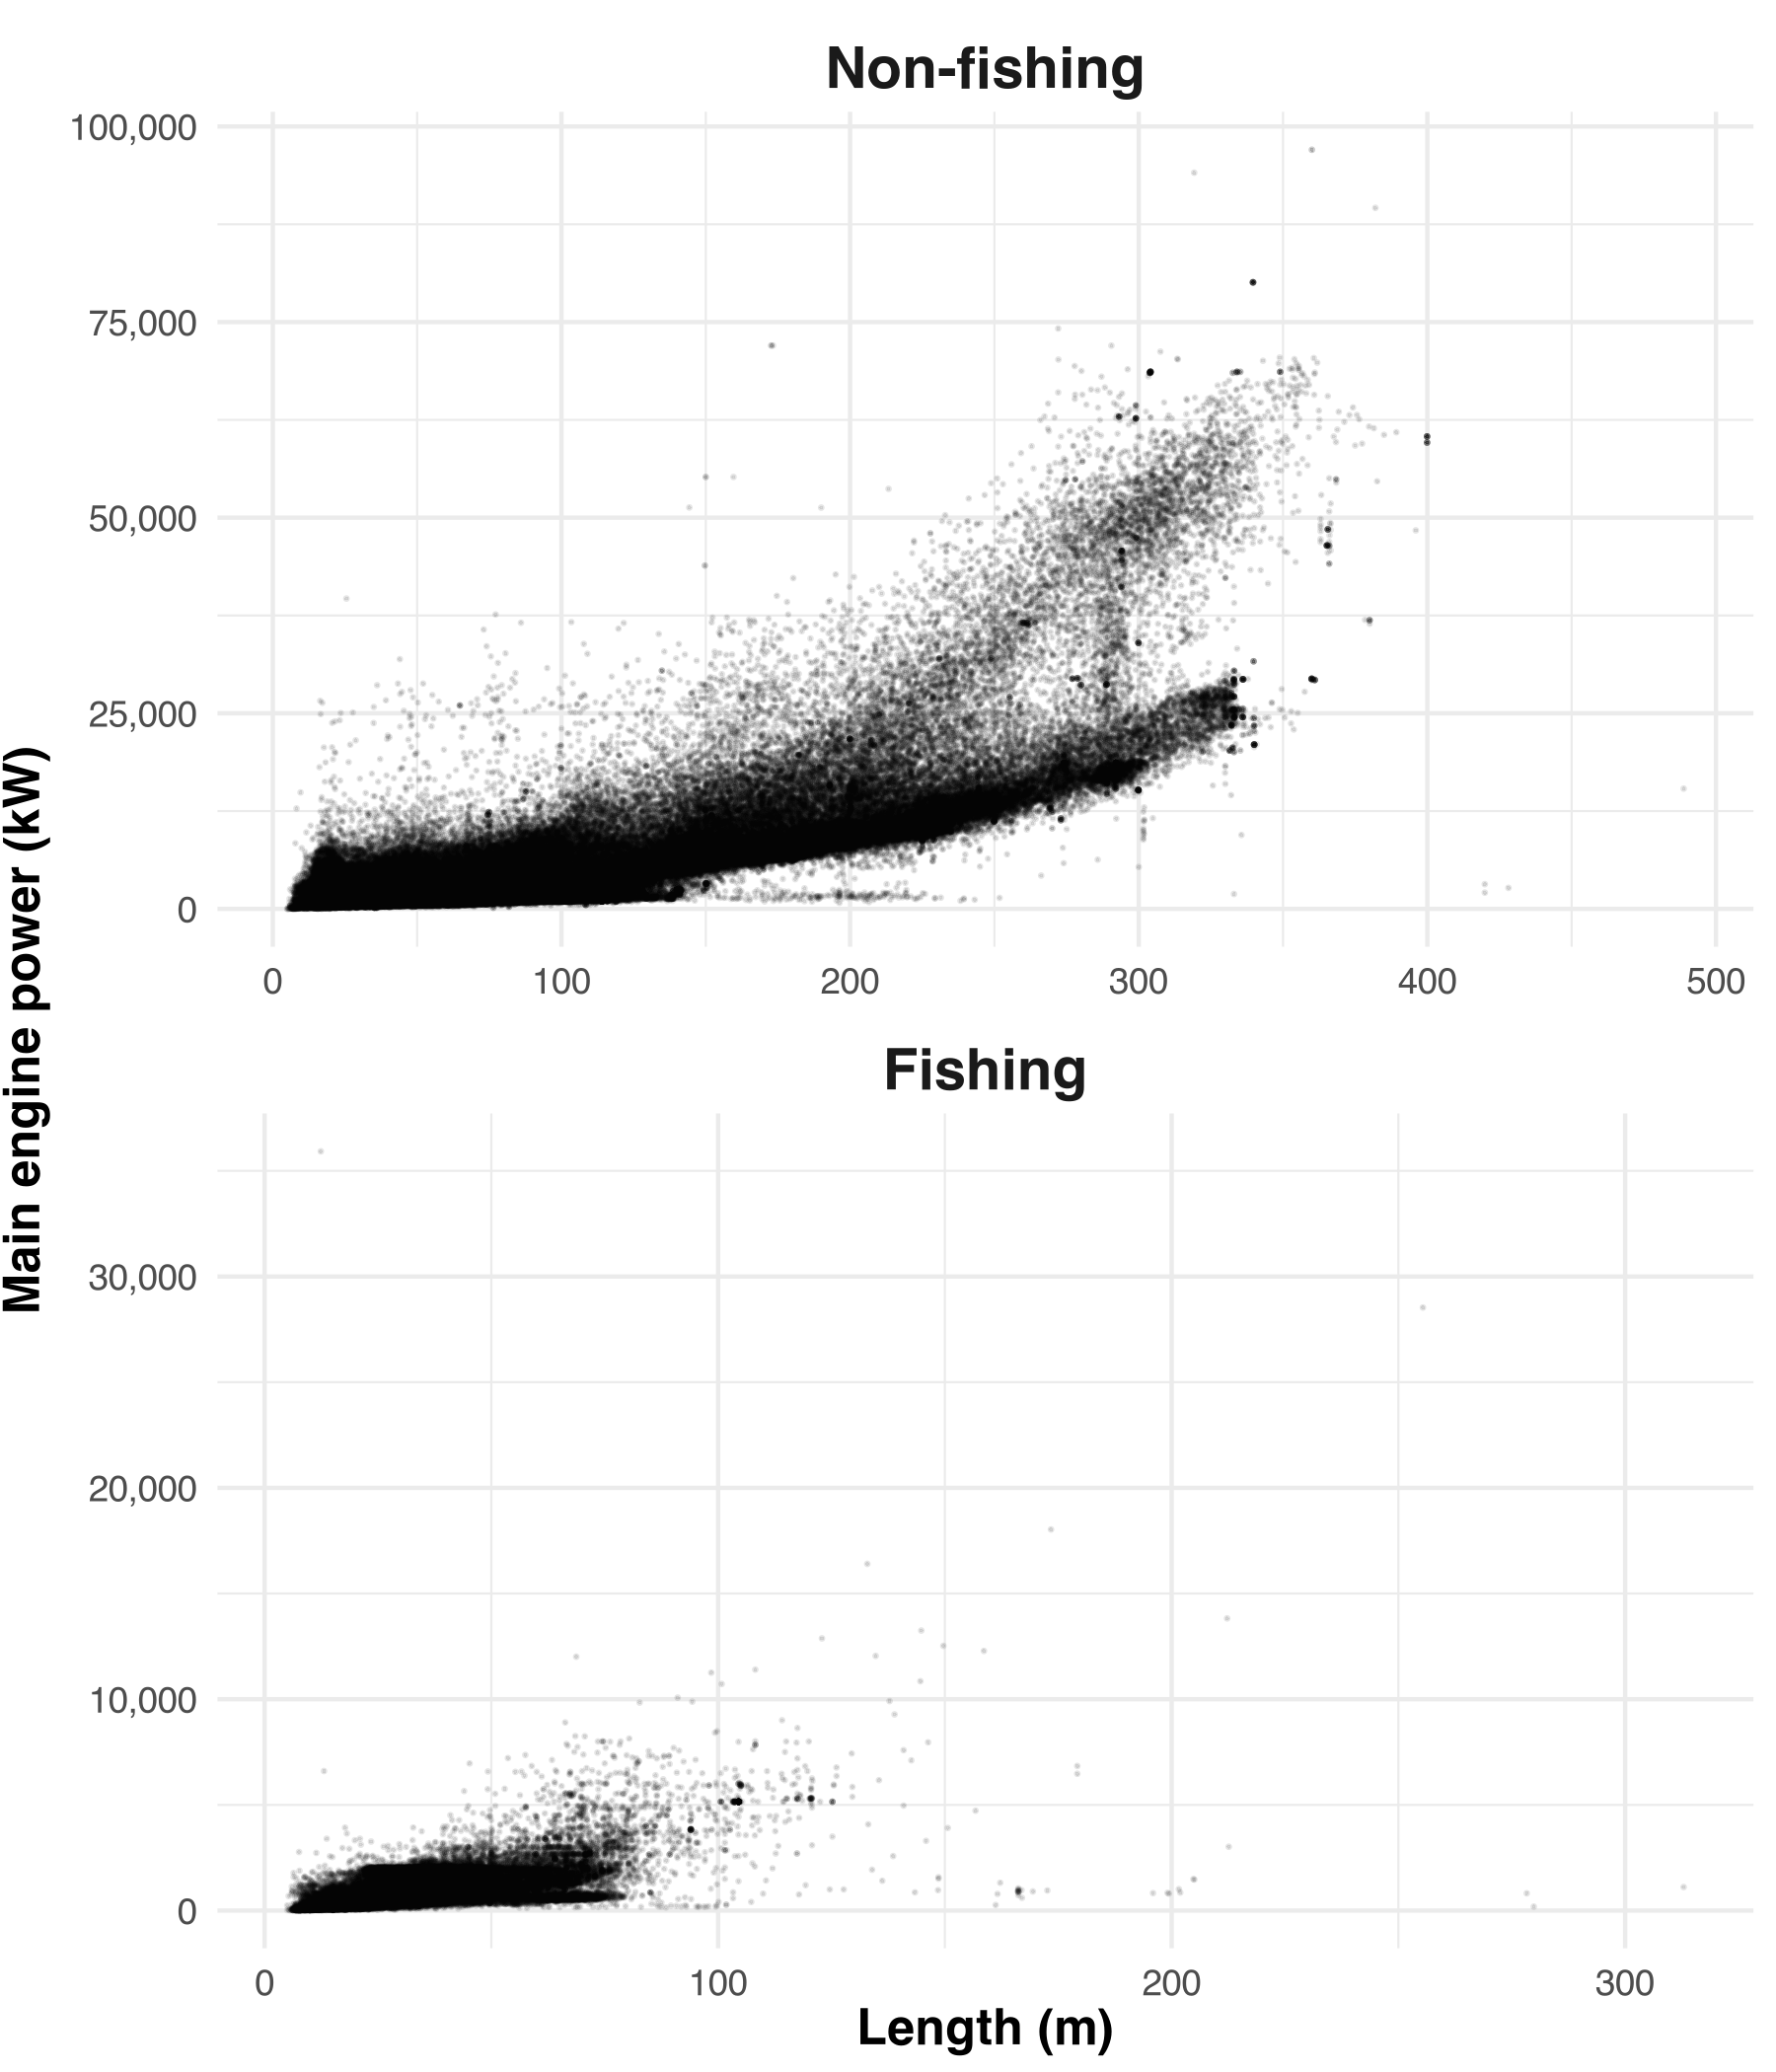
\includegraphics[width=\columnwidth]{figures/fig-ais-length-power-relationship-1.png}
    \caption{Relationship between main engine power (\DIFdelbeginFL \DIFdelFL{killowatts}\DIFdelendFL \DIFaddbeginFL \DIFaddFL{kilowatts}\DIFaddendFL ) and length (meters) for all AIS-broadcasting vessels, disaggregated by non-fishing and fishing vessels.}
    \label{fig:fig-ais-length-power-relationship}
\end{figure}

\paragraph{Detection classification}  Each observation unit is the boolean presence/absence of unmatched S1 detections in a given 1x1 degree ocean pixel, in a given month, for a given type of vessel (either non-fishing or fishing), for a given length bin.

\paragraph{Detection regression}  Each observation unit is the detection density of unmatched S1 detections in a given 1x1 degree ocean pixel, in a given month, for a given type of vessel (either non-fishing or fishing), for a given length bin. To calculate the detection density, we normalize detections by \DIFdelbegin \DIFdel{the total km² imaged across all }\DIFdelend S1 \DIFdelbegin \DIFdel{scenes }\DIFdelend \DIFaddbegin \DIFadd{sampling effort }\DIFaddend within each pixel and month\DIFdelbegin \DIFdel{to control for variation in Sentinel-1 sampling effort }\DIFdelend \DIFaddbegin \DIFadd{, defined as the imaged area of each individual S1 scene overlapping that pixel, summed across scenes. Because a pixel that is imaged on several passes contributes its imaged area once per pass, this quantity equals the area imaged at least once multiplied by the effective number of passes over it, and therefore carries units of km² × passes rather than km². Normalizing by it makes detection counts comparable across pixels and months, because S1 detections are anonymous and recorded per pass: a vessel that never moves is detected twice in a pixel imaged twice, and only dividing by an effort measure that counts both passes recovers the same density in each case}\DIFaddend .

\subsubsection{Model features}

We define a global spatial resolution of 1x1-degree which is used for all spatial model features, and use \DIFdelbegin \DIFdel{a }\DIFdelend monthly temporal units for all temporal model features. All model\DIFdelbegin \DIFdel{s}\DIFdelend  features used across the three models are summarized in Table \ref{tab:data_sources} and described below.

\clearpage

\begin{table}[!h]
\centering
\caption{\label{tab:data_sources}Data sources for all included model features, including which random forest model uses the features (M1: detections classification; M2: detections regression; and/or M3: emissions regression), the units, feature type, whether it varies spatially, whether it varies temporally, and the source name and reference citation.}
\centering
\fontsize{4}{6}\selectfont
\DIFdelbeginFL %DIFDELCMD < \begin{tabular}[t]{lllllllllll}
%DIFDELCMD < \toprule
%DIFDELCMD < Model feature & Category & M1 & M2 & M3 & Units & Type & Spatial & Temporal & Source & Ref.\\
%DIFDELCMD < \midrule
%DIFDELCMD < Presence/absence of unmatched S1 detections & Dependent variable & Yes & No & No & - & Boolean & Yes & Yes & GFW & \cite{paolo2024satellite}\\
%DIFDELCMD < Unmatched S1 detections per km2 imaged & Dependent variable & No & Yes & No & detects/km2 & Numeric & Yes & Yes & GFW & \cite{paolo2024satellite}\\
%DIFDELCMD < Log(AIS emissions) & Dependent variable & No & No & Yes & log(MT) & Numeric & Yes & Yes & GFW & -\\
%DIFDELCMD < Vessel type (fishing or non-fishing) & Dependent variable & Yes & Yes & Yes & - & Boolean & Yes & Yes & GFW & \cite{paolo2024satellite}\\
%DIFDELCMD < Lower threshold of vessel length bin & S1 detection features & Yes & Yes & No & m & Numeric & No & No & GFW & \cite{paolo2024satellite}\\
%DIFDELCMD < \addlinespace
%DIFDELCMD < Vessel length bin (4 categories) & S1 detection features & Yes & Yes & No & - & Factor & Yes & Yes & GFW & \cite{paolo2024satellite}\\
%DIFDELCMD < S1 detections per km$^2$ of area for each length bin & S1 detection features & No & No & Yes & detects/km2 & Numeric & Yes & Yes & GFW & \cite{paolo2024satellite}\\
%DIFDELCMD < Days since start of study & Temporal features & Yes & Yes & Yes & days & Numeric & No & Yes & GFW & \cite{kroodsma2018tracking}\\
%DIFDELCMD < Post-2020 IMO Sulphur policy & Temporal features & Yes & Yes & Yes & - & Boolean & No & Yes & IMO & \cite{imo_sulphur_2020}\\
%DIFDELCMD < Ocean basin & Geographic features  & Yes & Yes & Yes & - & Factor & Yes & No & GFW & \cite{kroodsma2018tracking}\\
%DIFDELCMD < \addlinespace
%DIFDELCMD < Pixel water area & Geographic features  & Yes & Yes & Yes & km2 & Numeric & Yes & No & GFW & \cite{paolo2024satellite}\\
%DIFDELCMD < Mean ocean depth & Geographic features  & Yes & Yes & Yes & m & Numeric & Yes & No & GFW & \cite{kroodsma2018tracking}\\
%DIFDELCMD < Mean distance from shore & Geographic features  & Yes & Yes & Yes & m & Numeric & Yes & No & GFW & \cite{kroodsma2018tracking}\\
%DIFDELCMD < Mean distance from nearest port & Geographic features  & Yes & Yes & Yes & m & Numeric & Yes & No & GFW & \cite{kroodsma2018tracking}\\
%DIFDELCMD < Distance to top 20 ports & Geographic features  & Yes & Yes & Yes & m & Numeric & Yes & No & Lloyd’s List & \cite{LloydsListTopPorts2024}\\
%DIFDELCMD < \addlinespace
%DIFDELCMD < Positions reported by AIS type a & AIS reception quality & Yes & Yes & Yes & - & Numeric & Yes & No & GFW & \cite{kroodsma2018tracking}\\
%DIFDELCMD < Positions reported by AIS type b & AIS reception quality & Yes & Yes & Yes & - & Numeric & Yes & No & GFW & \cite{kroodsma2018tracking}\\
%DIFDELCMD < Proportion of messages, dynamic AIS receivers & AIS reception quality & Yes & Yes & Yes & - & Numeric & Yes & Yes & GFW & \cite{kroodsma2018tracking}\\
%DIFDELCMD < Proportion of messages, terrestrial AIS receivers & AIS reception quality & Yes & Yes & Yes & - & Numeric & Yes & Yes & GFW & \cite{kroodsma2018tracking}\\
%DIFDELCMD < Proportion of messages, satellite AIS receivers & AIS reception quality & Yes & Yes & Yes & - & Numeric & Yes & Yes & GFW & \cite{kroodsma2018tracking}\\
%DIFDELCMD < \addlinespace
%DIFDELCMD < Mean wind speed & Weather features & Yes & Yes & Yes & m/s & Numeric & Yes & Yes & ERA5 & \cite{era5cds2023}\\
%DIFDELCMD < Mean primary wave height & Weather features & Yes & Yes & Yes & m & Numeric & Yes & Yes & ERA5 & \cite{era5cds2023}\\
%DIFDELCMD < Mean primary wave period & Weather features & Yes & Yes & Yes & s & Numeric & Yes & Yes & ERA5 & \cite{era5cds2023}\\
%DIFDELCMD < \bottomrule
%DIFDELCMD < \end{tabular}
%DIFDELCMD < %%%
\DIFdelendFL \DIFaddbeginFL \setlength{\tabcolsep}{2pt}
\begin{tabular}[t]{lllllllllll}
\toprule
Model feature & Category & M1 & M2 & M3 & Units & Type & Spatial & Temporal & Source & Ref.\\
\midrule
Presence/absence of unmatched S1 detections & Dependent variable & Yes & No & No & - & Boolean & Yes & Yes & GFW & \cite{paolo2024satellite}\\
Unmatched S1 detections per km2 imaged & Dependent variable & No & Yes & No & detects/km2 & Numeric & Yes & Yes & GFW & \cite{paolo2024satellite}\\
Log(AIS emissions) & Dependent variable & No & No & Yes & log(MT) & Numeric & Yes & Yes & GFW & -\\
Vessel type (fishing or non-fishing) & Dependent variable & Yes & Yes & Yes & - & Boolean & Yes & Yes & GFW & \cite{paolo2024satellite}\\
Lower threshold of vessel length bin & S1 detection features & Yes & Yes & No & m & Numeric & No & No & GFW & \cite{paolo2024satellite}\\
\addlinespace
Vessel length bin category & S1 detection features & Yes & Yes & No & - & Factor & Yes & Yes & GFW & \cite{paolo2024satellite}\\
S1 detections per km$^2$ of area for each length bin & S1 detection features & No & No & Yes & detects/km2 & Numeric & Yes & Yes & GFW & \cite{paolo2024satellite}\\
Total pixel area imaged by S1 across all time & S1 detection features & Yes & Yes & No & km2 & Numeric & Yes & No & GFW & \cite{paolo2024satellite}\\
Unique AIS-broadcasting vessels in pixel-month & AIS reception quality & Yes & Yes & No & - & Numeric & Yes & Yes & GFW & \cite{kroodsma2018tracking}\\
Unique AIS-broadcasting vessels globally & AIS reception quality & Yes & Yes & No & - & Numeric & No & Yes & GFW & \cite{kroodsma2018tracking}\\
\addlinespace
Positions reported by AIS type A & AIS reception quality & Yes & Yes & Yes & - & Numeric & Yes & No & GFW & \cite{kroodsma2018tracking}\\
Positions reported by AIS type B & AIS reception quality & Yes & Yes & Yes & - & Numeric & Yes & No & GFW & \cite{kroodsma2018tracking}\\
Proportion of messages, dynamic AIS receivers & AIS reception quality & Yes & Yes & Yes & - & Numeric & Yes & Yes & GFW & \cite{kroodsma2018tracking}\\
Proportion of messages, terrestrial AIS receivers & AIS reception quality & Yes & Yes & Yes & - & Numeric & Yes & Yes & GFW & \cite{kroodsma2018tracking}\\
Proportion of messages, satellite AIS receivers & AIS reception quality & Yes & Yes & Yes & - & Numeric & Yes & Yes & GFW & \cite{kroodsma2018tracking}\\
\addlinespace
Month of year & Temporal features & Yes & Yes & Yes & - & Factor & No & Yes & GFW & -\\
Post-2020 IMO sulfur policy & Temporal features & No & No & Yes & - & Boolean & No & Yes & IMO & \cite{imo_sulphur_2020}\\
Ocean basin & Geographic features  & Yes & Yes & Yes & - & Factor & Yes & No & GFW & \cite{kroodsma2018tracking}\\
Pixel water area & Geographic features  & Yes & Yes & Yes & km2 & Numeric & Yes & No & GFW & \cite{paolo2024satellite}\\
Pixel water fraction & Geographic features & No & No & Yes & - & Numeric & Yes & No & GFW & \cite{paolo2024satellite}\\
\addlinespace
Mean ocean depth & Geographic features  & Yes & Yes & Yes & m & Numeric & Yes & No & GFW & \cite{kroodsma2018tracking}\\
Mean distance from shore & Geographic features  & Yes & Yes & Yes & m & Numeric & Yes & No & GFW & \cite{kroodsma2018tracking}\\
Mean distance from nearest port & Geographic features  & Yes & Yes & Yes & m & Numeric & Yes & No & GFW & \cite{kroodsma2018tracking}\\
Minimum distance to top 20 port & Geographic features  & Yes & Yes & Yes & m & Numeric & Yes & No & Lloyd’s List & \cite{LloydsListTopPorts2024}\\
\bottomrule
\end{tabular}
\DIFaddendFL \end{table}
\DIFaddbegin \FloatBarrier
\DIFaddend 

\clearpage

\paragraph{S1 vessel detection features}

For the emissions regression model, we include several model features that capture the vessel length frequency distribution of S1 detections that occurred in any given pixel-month for each vessel type (fishing or non-fishing). \DIFdelbegin \DIFdel{This prevents assigning emissions to vessels for which no emission estimates are available. }\DIFdelend S1 detections smaller than the minimum vessel size represented in the AIS-broadcasting dataset are excluded to avoid assigning emissions to vessel sizes not characterized by the AIS emissions model. We normalize the detections by the \DIFdelbegin \DIFdel{total km² imaged }\DIFdelend \DIFaddbegin \DIFadd{same measure of S1 sampling effort described above (per-scene imaged area summed }\DIFaddend across all S1 scenes within each pixel-month\DIFaddbegin \DIFadd{, in km² × passes) }\DIFaddend to account for spatiotemporal variation in S\DIFdelbegin \DIFdel{entinel-}\DIFdelend 1 sampling effort and therefore create a measure of detection density (Fig. \ref{fig:fig-map-fraction-months-imaged} shows spatial variation of sampling effort; Fig. \ref{fig:fig-s1-coverage-time-series} shows temporal variation). The \DIFaddbegin \DIFadd{loss of the Sentinel-1B satellite in December 2021 provides a test of this normalization: it cut the number of S1 scenes by 38\% from 2021 to 2022, but vessel detections per unit of imaged area changed by less than 1\% (Fig. \ref{fig:fig-s1-coverage-time-series}b,c). The }\DIFaddend emissions regression model is trained with these features corresponding to matched detection density in order to predict \DIFdelbegin \DIFdel{AIS-broadcasting }\DIFdelend \DIFaddbegin \DIFadd{AIS-based }\DIFaddend emissions; when it comes time for using the model to predict \DIFdelbegin \DIFdel{non-broadcasting }\DIFdelend \DIFaddbegin \DIFadd{S1-unmatched }\DIFaddend emissions, the unmatched detection density is used for these features instead.

For the detection classification and detection regression models, each unit of observation represents one of the vessel length bins for each pixel-month and vessel type. We also include two model features describing the length bin for each observation: the numeric lower threshold for the vessel length bin, and a categorical factor representing which of the length bins the observation belongs to. \DIFaddbegin \DIFadd{We finally include for each pixel the total S1 sampling effort accumulated across the entire 2017-2025 time period, again summed across scenes, in order to account for the general amount each pixel is imaged. 
}\DIFaddend 


\DIFdelbegin %DIFDELCMD < \begin{figure}[H]
%DIFDELCMD <     \centering    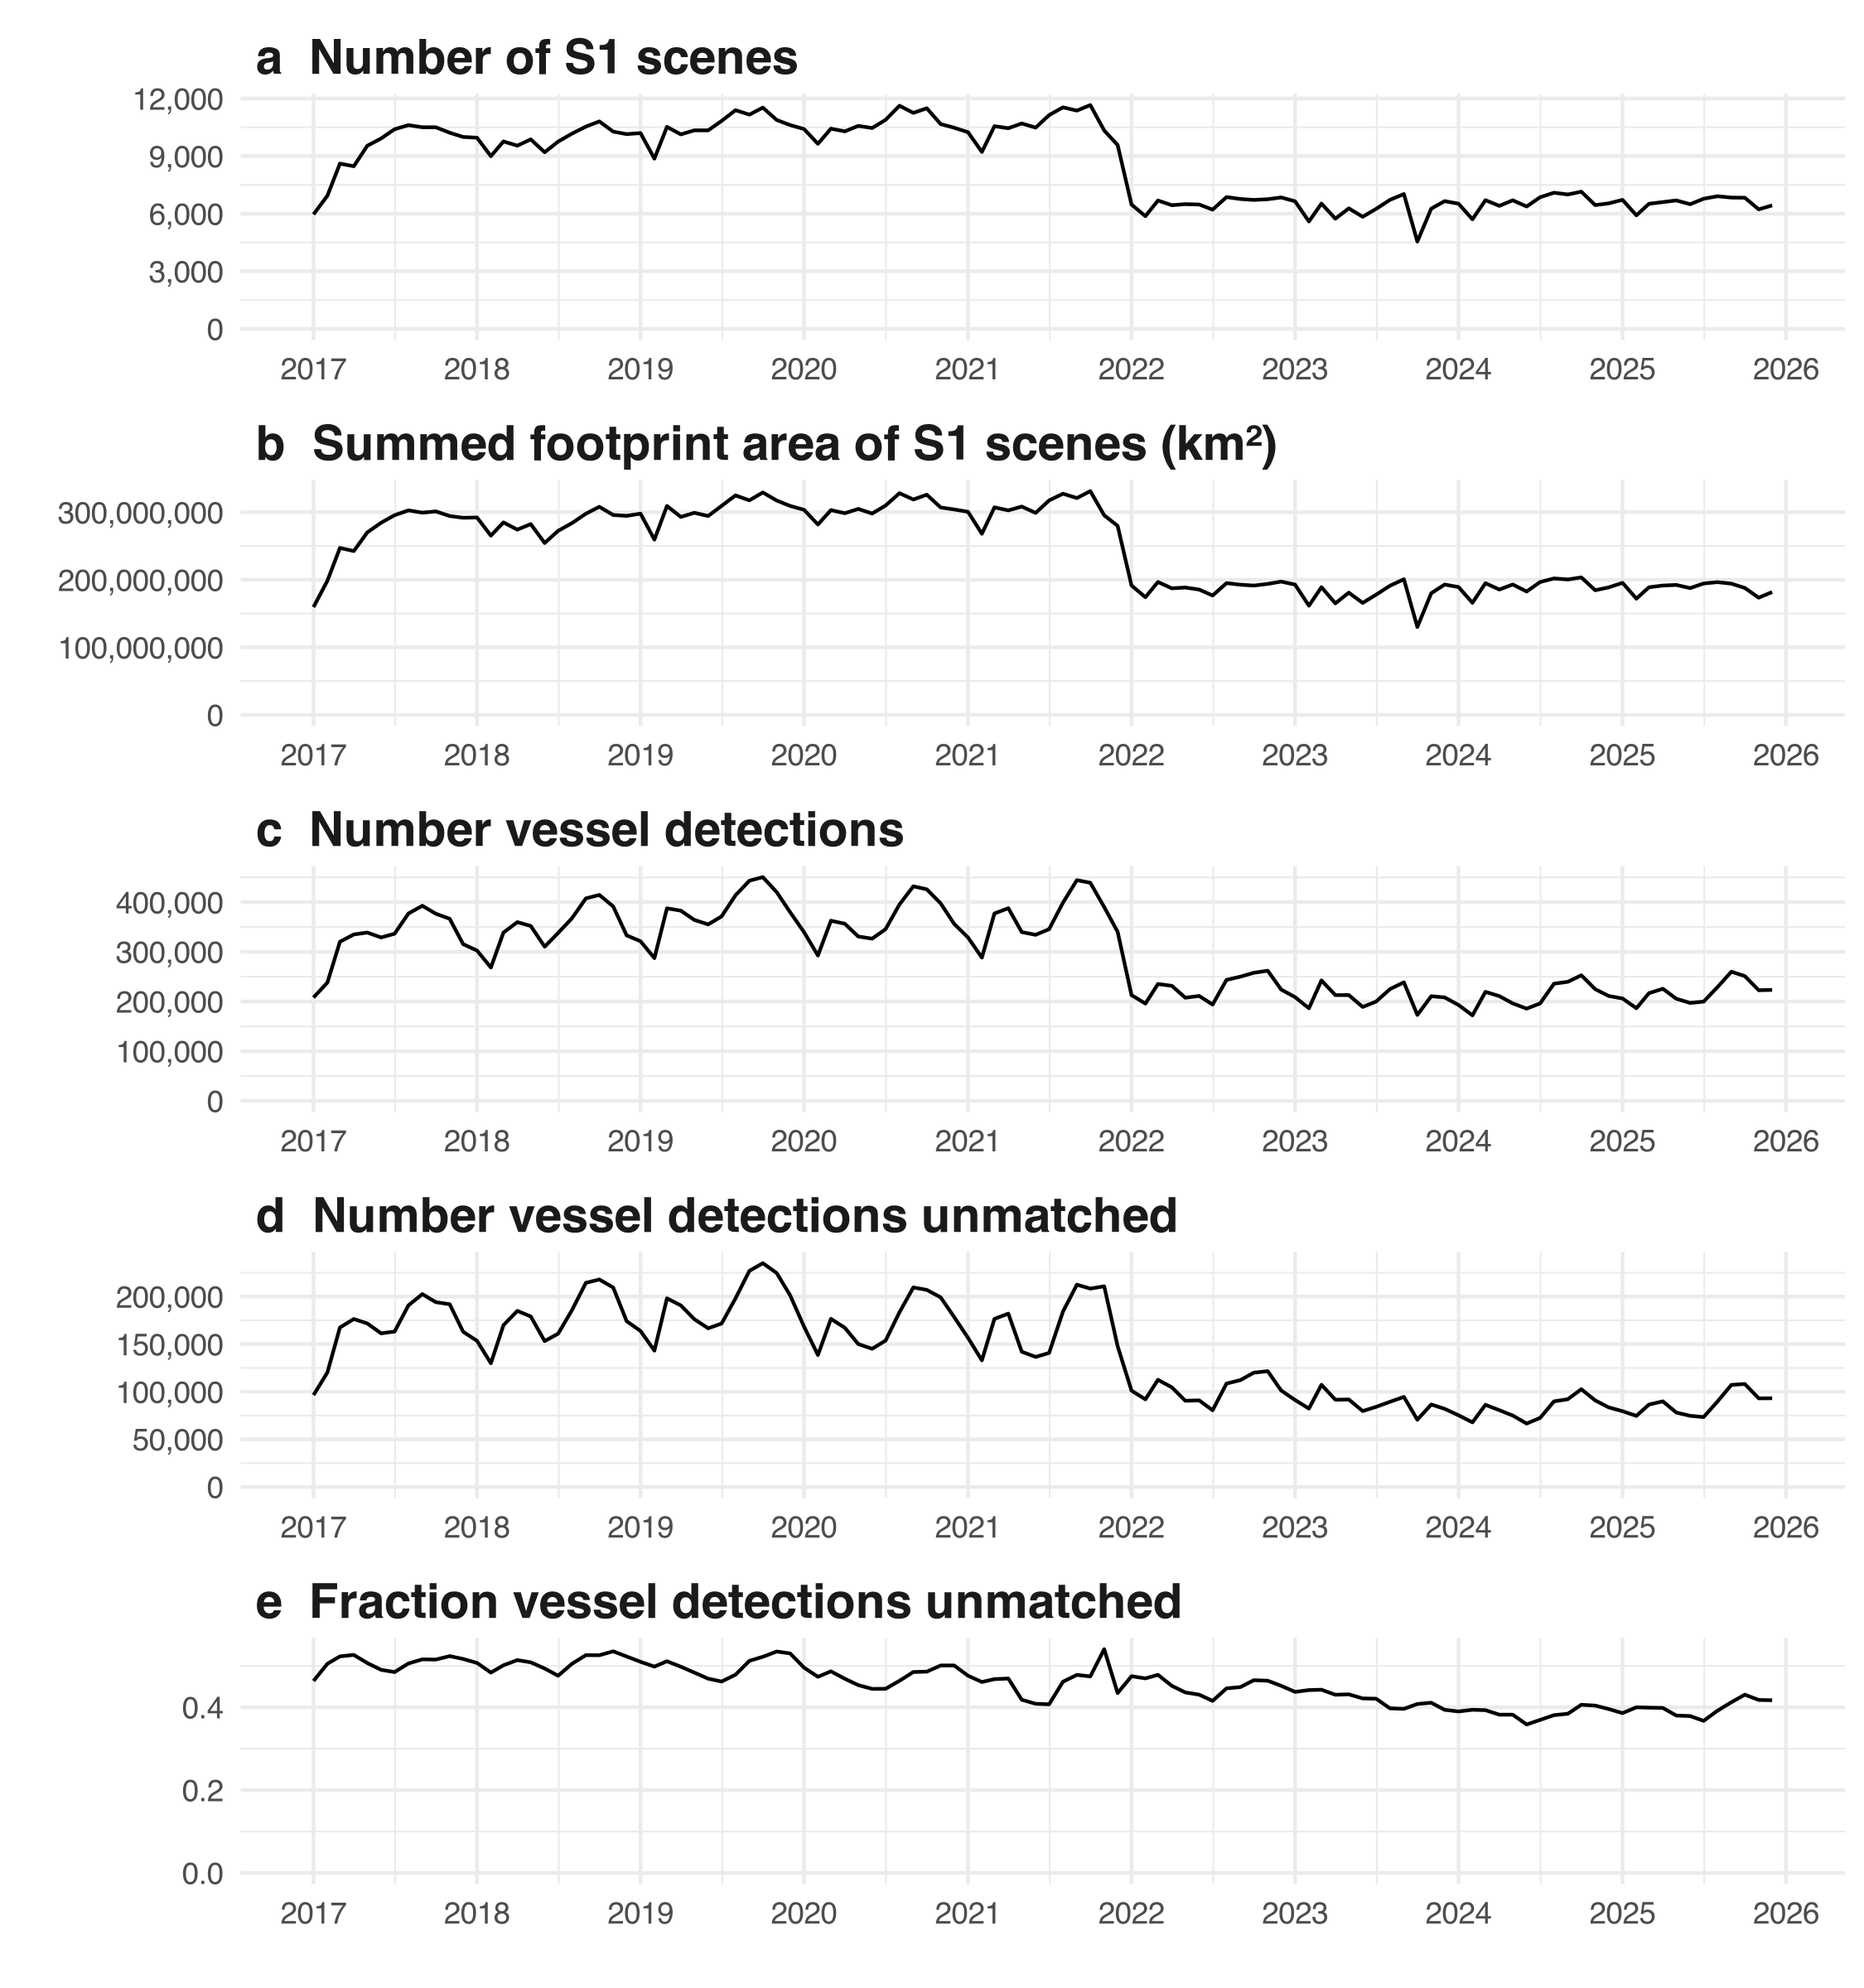
\includegraphics[width=\columnwidth]{figures/fig-s1-coverage-time-series-1.png}
%DIFDELCMD <     %%%
%DIFDELCMD < \caption{%
{%DIFAUXCMD
\DIFdelFL{Monthly statistics of global S1 coverage including total number of S1 scenes, total imaged area across all S1 scenes, total number of vessel detections, total number of vessel detections that could not be matched to an AIS-broadcasting vessels, and fraction of the total number of vessel detections that could not be matched to an AIS-broadcasting vessels.}}
    %DIFAUXCMD
%DIFDELCMD < \label{fig:fig-s1-coverage-time-series}
%DIFDELCMD < \end{figure}
%DIFDELCMD < 

%DIFDELCMD < %%%
\DIFdelend \paragraph{Spatial features}

For each pixel we extract spatial information, including depth, distance to shore, and distance to the nearest port, from a high-resolution GFW subproduct (0.01x0.01-degree) and aggregate it to our 1x1-degree grid resolution by computing the minimum value in each pixel. In addition to the distance from the nearest port (which can be of any size port), we also include the distance from each pixel centroid to the nearest of the top 20 container ports according to the Lloyd's list of 2024 \cite{LloydsListTopPorts2024}. We include this since traffic density, loitering practices, and navigation behavior in major ports differ from those in regular ports. Additional geographic features include the \DIFdelbegin \DIFdel{water }\DIFdelend \DIFaddbegin \DIFadd{total area covered by water within each pixel, the fraction of }\DIFaddend area within each pixel \DIFdelbegin \DIFdel{(excluding land and the 1 km S1 buffer from shore) and }\DIFdelend \DIFaddbegin \DIFadd{covered by water, and }\DIFaddend a categorical variable indicating which of the five major ocean basins each pixel falls within.

\DIFdelbegin \paragraph{\DIFdel{Weather features}}
%DIFAUXCMD
\addtocounter{paragraph}{-1}%DIFAUXCMD
%DIFDELCMD < 

%DIFDELCMD < %%%
\DIFdel{Weather may influence both emissions and S1 detections. Sea conditions may affect not only vessel presence (e.g., smaller vessels may remain in port during storms), but also navigation behavior \mbox{%DIFAUXCMD
\cite{majamaki2025improving}}\hskip0pt%DIFAUXCMD
. In addition, sea surface waves generated by wind modify SAR background signal, directly affecting the ability of the S1 detection model to accurately identify vessels \mbox{%DIFAUXCMD
\cite{huo2018ship}}\hskip0pt%DIFAUXCMD
. To account for these effects, we extracted weather data from ECMWF Reanalysis v5 (ERA5), the fifth-generation atmospheric reanalysis of the global climate, produced by the Copernicus Climate Change Service \mbox{%DIFAUXCMD
\cite{era5cds2023}}\hskip0pt%DIFAUXCMD
. We used Google Earth Engine to extract hourly ERA5 data and aggregate it to monthly minimum, maximum, and average values. Because ERA5 has higher spatial resolution than our 1×1-degree grid, we re-aggregated the data for each pixel, excluding land and the 1 km S1 buffer from shore, computing the mean of the monthly minimum, maximum, and average values, as well as the overall minimum and maximum across all sub-pixels (i.e., five values for each parameter). As our final model features, we used mean wind speed (which influences both navigation conditions and S1 detection), mean swell height (which affect navigation and vessel activity), and mean swell period (which also affect navigation and vessel activity).
}%DIFDELCMD < 

%DIFDELCMD < %%%
\DIFdelend \paragraph{AIS reception quality features}

We included several model features related to AIS reception quality and signal type. To account for reception quality, we used two features: messages per day for AIS \DIFdelbegin \DIFdel{Type A and Type }\DIFdelend \DIFaddbegin \DIFadd{Class A and Class }\DIFaddend B transponders, capturing regional variation in AIS reception. Additionally, because AIS signals are received via different systems (terrestrial receivers, satellite receivers, and more recently dynamic receivers) we identified the associated receiver type for each ping and calculated the proportion of each type per pixel and month, summing to one. These features describing AIS coverage and the predominance of receiver types influence the fraction of broadcasting versus non-broadcasting vessels, and thus the associated emissions and detections.

\paragraph{Temporal features}

To account for temporal variability in each of the three models, we include a \DIFdelbegin \DIFdel{numeric feature representing days since the start of the study period (January 1, 2017)}\DIFdelend \DIFaddbegin \DIFadd{factor feature representing the month of the year}\DIFaddend . We also include a boolean feature for whether or not the observation occurs on or after January 2020, to coincide with the start of the IMO low \DIFdelbegin \DIFdel{sulphur }\DIFdelend \DIFaddbegin \DIFadd{sulfur }\DIFaddend fuel policy. \DIFaddbegin \DIFadd{To account for temporal trends of general vessel activity in the detection classification and regression models, we include features characterizing the total number of unique AIS-broadcasting vessels globally each month, as well as the number of unique AIS-broadcasting vessels in each pixel-month. }\DIFaddend Accounting for temporal variation is particularly important given \DIFaddbegin \DIFadd{both }\DIFaddend the variation in S1 coverage over time\DIFaddbegin \DIFadd{, as well as the variation in global fleet composition over time }\DIFaddend (Fig. \ref{fig:fig-s1-coverage-time-series}).

\subsubsection{Data pre-processing}

We perform the following data pre-processing steps, in this order, each time a model is trained or predictions are inferred. In order to avoid data leakage during performance testing, data pre-processing that performs calculations that directly use the data (i.e., imputation of missing values) is always performed  on the training data. To do so, we leverage the recipes package in R \cite{recipes}.

1. We treat several features as categorical (fishing or non-fishing; the post-2020 temporal boolean; ocean; and for the detection classification and regression models that are disaggregated by vessel length bin, we treat the length bin as categorical)

2. \DIFdelbegin \DIFdel{We remove any numeric model features that have near-zero variance
}%DIFDELCMD < 

%DIFDELCMD < %%%
\DIFdel{3. }\DIFdelend For any missing values of numeric model features, we impute their value using the median of that feature's non-missing values.

\DIFdelbegin \DIFdel{4. }\DIFdelend \DIFaddbegin \DIFadd{3. }\DIFaddend We remove any numeric model features that are highly correlated with other features (i.e., that have a Pearson's correlation coefficient of $>$ 0.9).

\subsubsection{Model training}

We defined three independent Random Forest models using the tidymodels framework in R \cite{tidymodels}. Model fitting was done using the ranger engine \cite{ranger} in parsnip \cite{parsnip}. We  use 500 trees for each forest, and otherwise use default hyperparameter settings for ranger. We perform several out-of-sample performance tests for each model using independent training and testing data splits to assess how well it does for predictions inside the S1 footprint, as well as a simulation of how well it would do for predictions outside the footprint. We train each of the three final models using the entire dataset.

For the detection presence/absence classification model, we use an additional validation dataset to optimize the classification cutoff threshold to maximize the F1 score (the harmonic mean of precision and recall). So for performance tests, we train the model on a training dataset, calibrate the classification threshold on the validation dataset, and then test performance on the testing dataset using the optimized threshold. For the final model, we train the model using a training dataset, calibrate the classification threshold on a validation dataset, and then train a final model using the entire dataset and the optimized threshold.

For the eight linear regression models to convert CO$_2$ emissions to emissions of other GHGs and pollutants, we use the lm function from the base R stats package \cite{r}.

\subsubsection{Model testing}

We assessed model performance for each of the three models using two different evaluation approaches designed to test: 1) predictive power for areas within the S1 footprint but that don't have overpasses in a given month (subsequently referred to as our \DIFdelbegin \DIFdel{'}\DIFdelend \DIFaddbegin \DIFadd{`}\DIFaddend inside footprint' test); and 2) the models' ability to generalize to locations completely outside the S1 footprint (subsequently referred to as our \DIFdelbegin \DIFdel{'}\DIFdelend \DIFaddbegin \DIFadd{`}\DIFaddend simulated outside footprint' test).

\paragraph{Inside S1 footprint testing}

Because both emissions and detection predictions inside the S1 footprint are made for locations where emissions and detections data is available for training, (i.e., inside the footprint we are not generalizing to regions with unknown emissions and detections), we first evaluated performance inside the footprint using a stratified random $80\%$/$20\%$ training/testing split. For each of the three models, we stratify the random split by the dependent variable (presence/absence of unmatched detections for the detections classification model; density of unmatched detections for the detections regression model; and log-transformed emissions for the emissions regression model). 

For the detection presence/absence classification model, we use an additional validation dataset to optimize the classification cutoff threshold. In this case, we use a $60\%$/$20\%$/$20\%$ training/ validation/ testing split.

\paragraph{Simulated outside S1 footprint testing}

Then, to assess spatial transferability when predicting emissions in areas completely outside the S1 footprint (i.e., areas far from shore), we implement a spatially structured split, training on nearshore pixels (\DIFdelbegin \DIFdel{$<=$ 100km from shore}\DIFdelend \DIFaddbegin \DIFadd{$\le$ 100 km from the nearest port}\DIFaddend ) and testing on offshore pixels ($>$ \DIFdelbegin \DIFdel{100km from shore}\DIFdelend \DIFaddbegin \DIFadd{100 km from the nearest port}\DIFaddend ) (Fig. \ref{fig:fig-offshore-outside-footprint-training-testing-map}). 

For the detection presence/absence classification model, we again use an additional validation dataset to optimize the classification cutoff threshold. We therefore use data from nearshore pixels to create a stratified random $80\%$/$20\%$ training/validation split, and then test using the offshore pixels.


\begin{figure}[H]
    \centering    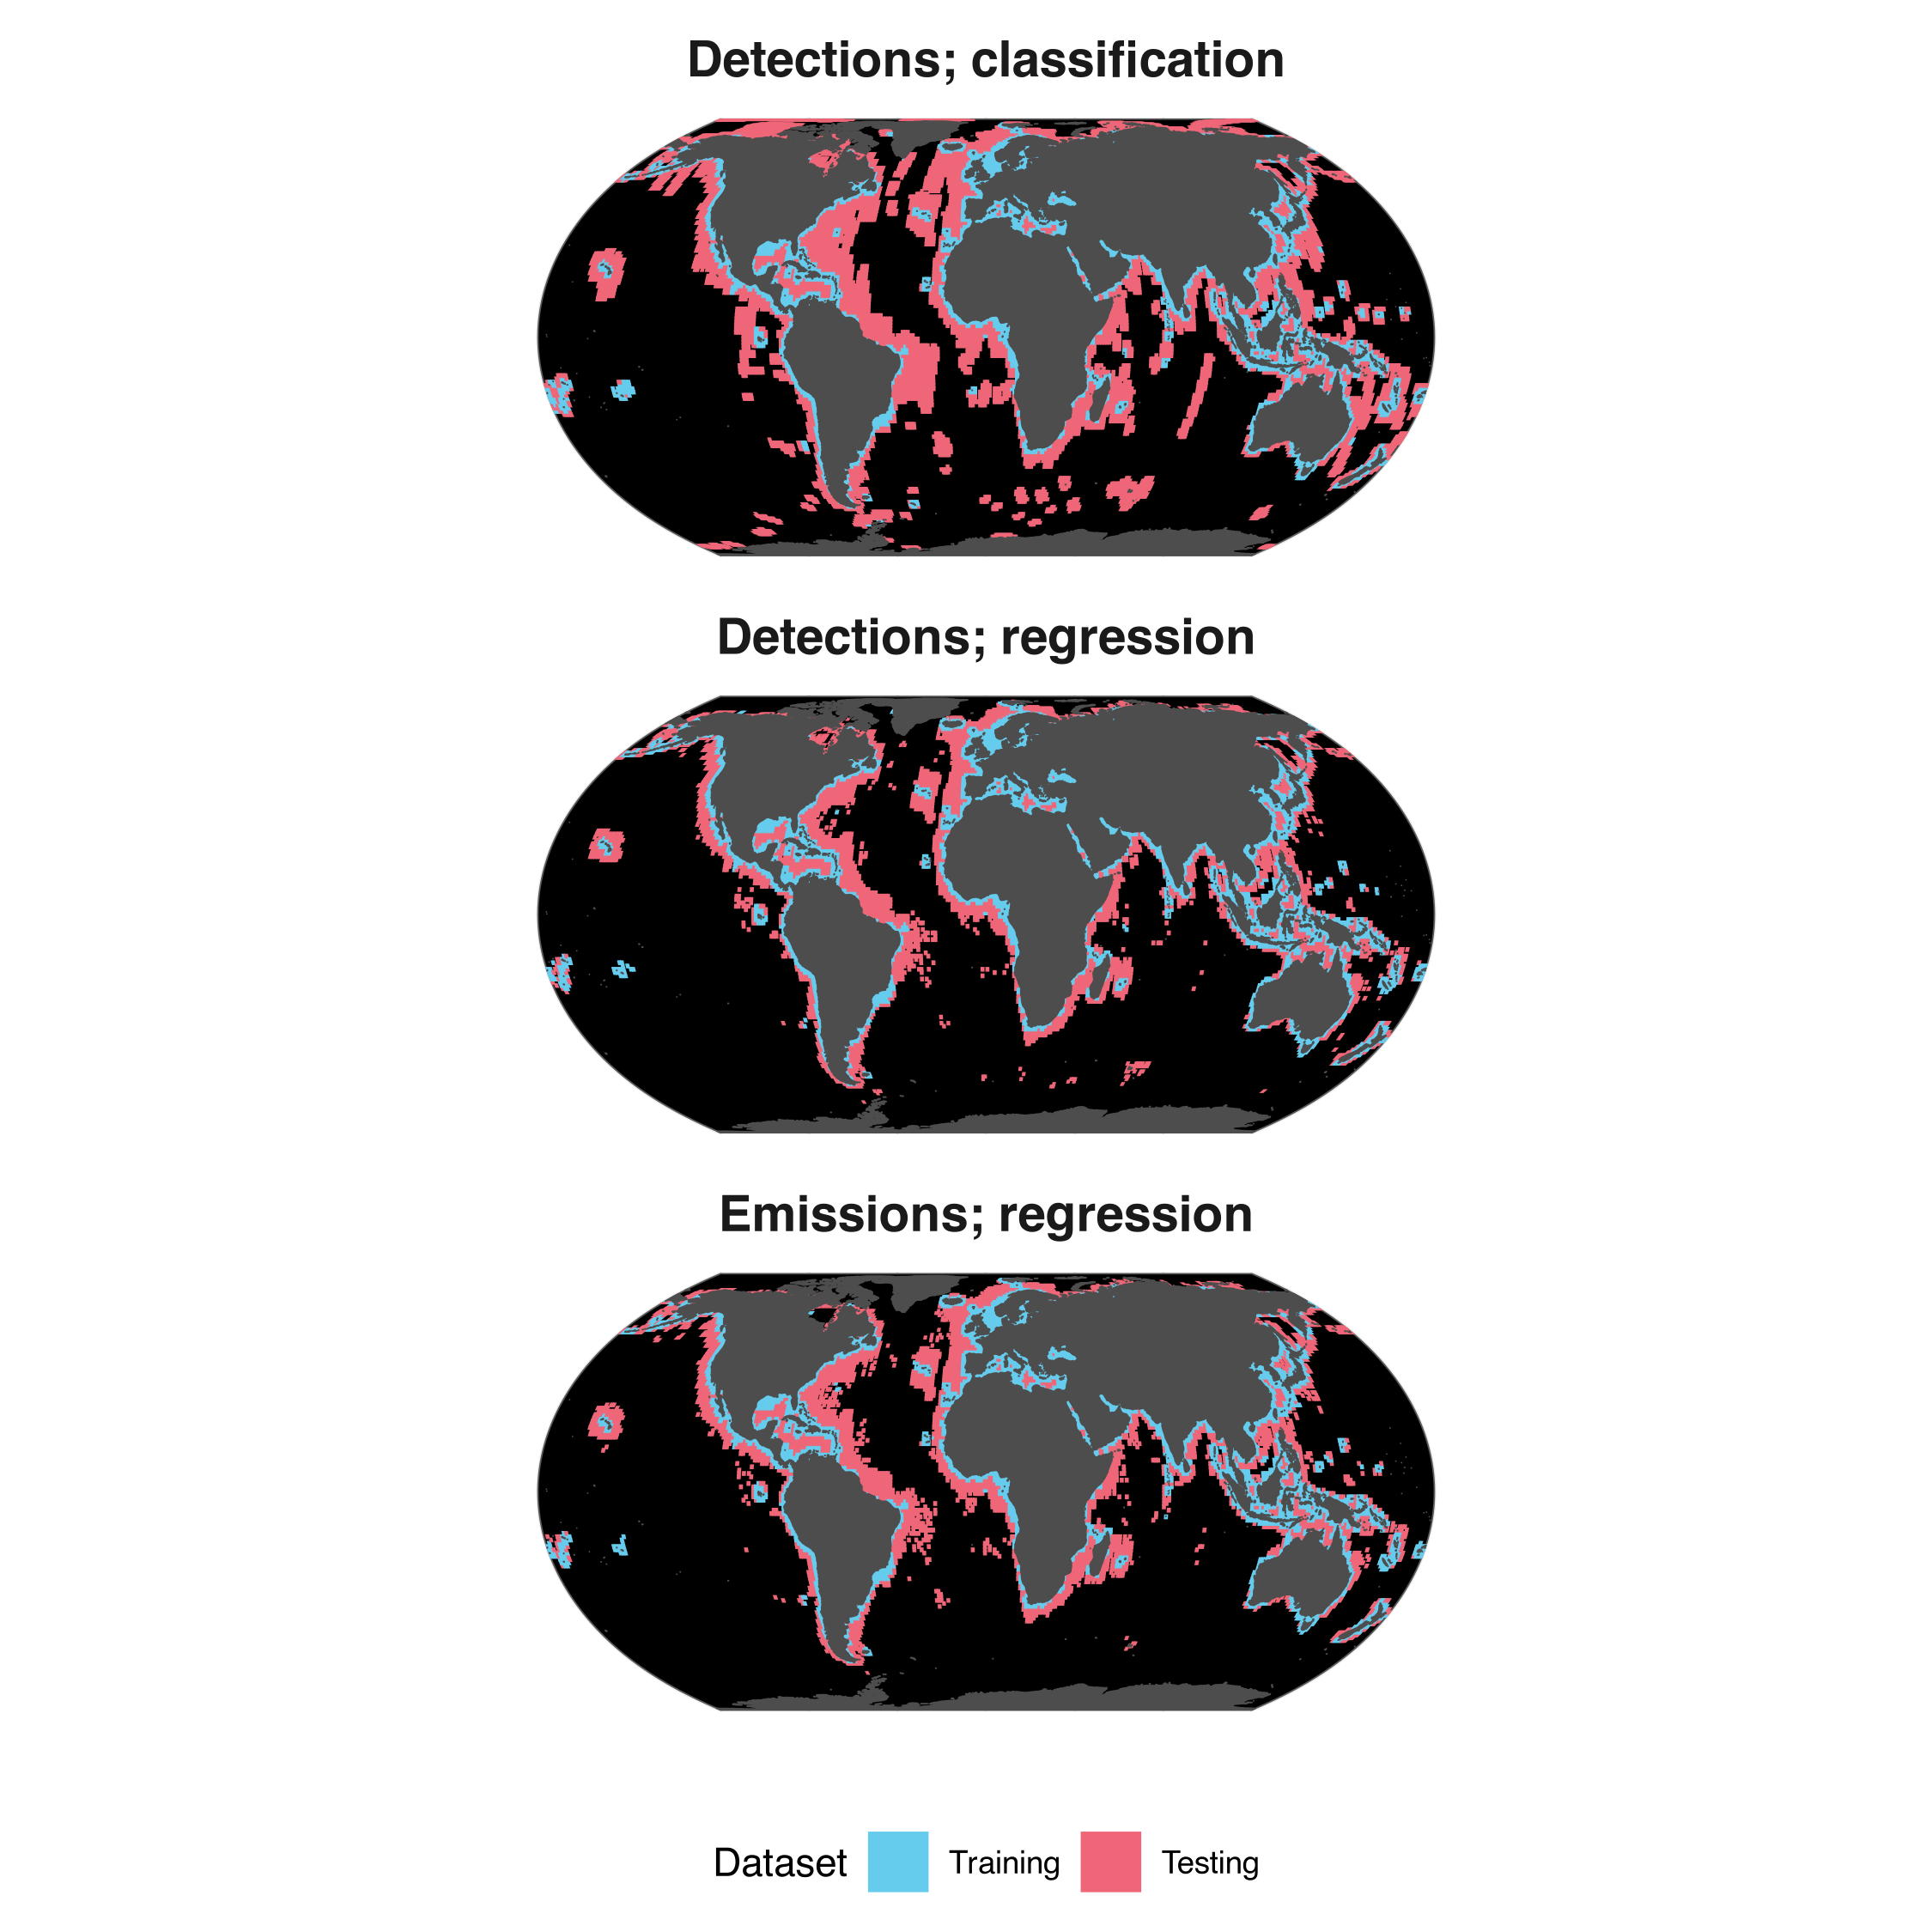
\includegraphics[width=\columnwidth]{figures/fig-offshore-outside-footprint-training-testing-map-1.png}
    \caption{Maps of pixels that were used in the training and testing datasets for the simulated outside S1 footprint performance tests for each model. Pixels \DIFdelbeginFL \DIFdelFL{$<=$ 100km }\DIFdelendFL \DIFaddbeginFL \DIFaddFL{$\le$ 100 km }\DIFaddendFL from the \DIFdelbeginFL \DIFdelFL{shore }\DIFdelendFL \DIFaddbeginFL \DIFaddFL{nearest port }\DIFaddendFL were used for training; pixels $>$ \DIFdelbeginFL \DIFdelFL{100km }\DIFdelendFL \DIFaddbeginFL \DIFaddFL{100 km }\DIFaddendFL from \DIFdelbeginFL \DIFdelFL{shore }\DIFdelendFL \DIFaddbeginFL \DIFaddFL{the nearest port }\DIFaddendFL were used for testing.}
    \label{fig:fig-offshore-outside-footprint-training-testing-map}
\end{figure}

Classifier performance is reported using precision-recall curves (Fig. \ref{fig:fig-pr-curves}), receiver operating characteristic (ROC) curves (Fig. \ref{fig:fig-roc-curves}), and confusion matrices (Fig. \ref{fig:fig-conf-mat}). Table \ref{tab:all_performance_metrics_table} also summarizes regression performance for detections, both inside and outside the footprint, alongside the emissions model performance. To assess the performance of the emissions model, predicted log emissions were back-transformed using Duan’s smearing coefficient, calculated from the residuals of the training data \cite{duan1983smearing}. The same transformation was applied to the final model prediction.

For the CO$_2$ emissions regression random forest, we simply train the model on the training data and test the model on the testing data (using the two sets of splits described above for inside and outside the S1 footprint tests). For the other eight gases, we: 1) train the linear regression using the training data (to convert CO$_2$ emissions to emissions of each gas); 2) use the CO$_2$ emissions regression random forest to predict emissions for the testing data; and then 3) use the predicted CO$_2$ emissions for the testing data and then convert this to emissions for each of the other eight gases using the eight linear regressions built in step \DIFdelbegin \DIFdel{2}\DIFdelend \DIFaddbegin \DIFadd{1}\DIFaddend ; and then 4) compare the predicted emissions of each of the eight gases against the observed emissions of each of the eight gases in the \DIFdelbegin \DIFdel{training }\DIFdelend \DIFaddbegin \DIFadd{testing }\DIFaddend data. In this way, we are able to measure fully out-of-sample performance for predicting not only CO$_2$, but also all of the other two GHGs and six pollutants.


\begin{figure}[H]
    \centering
    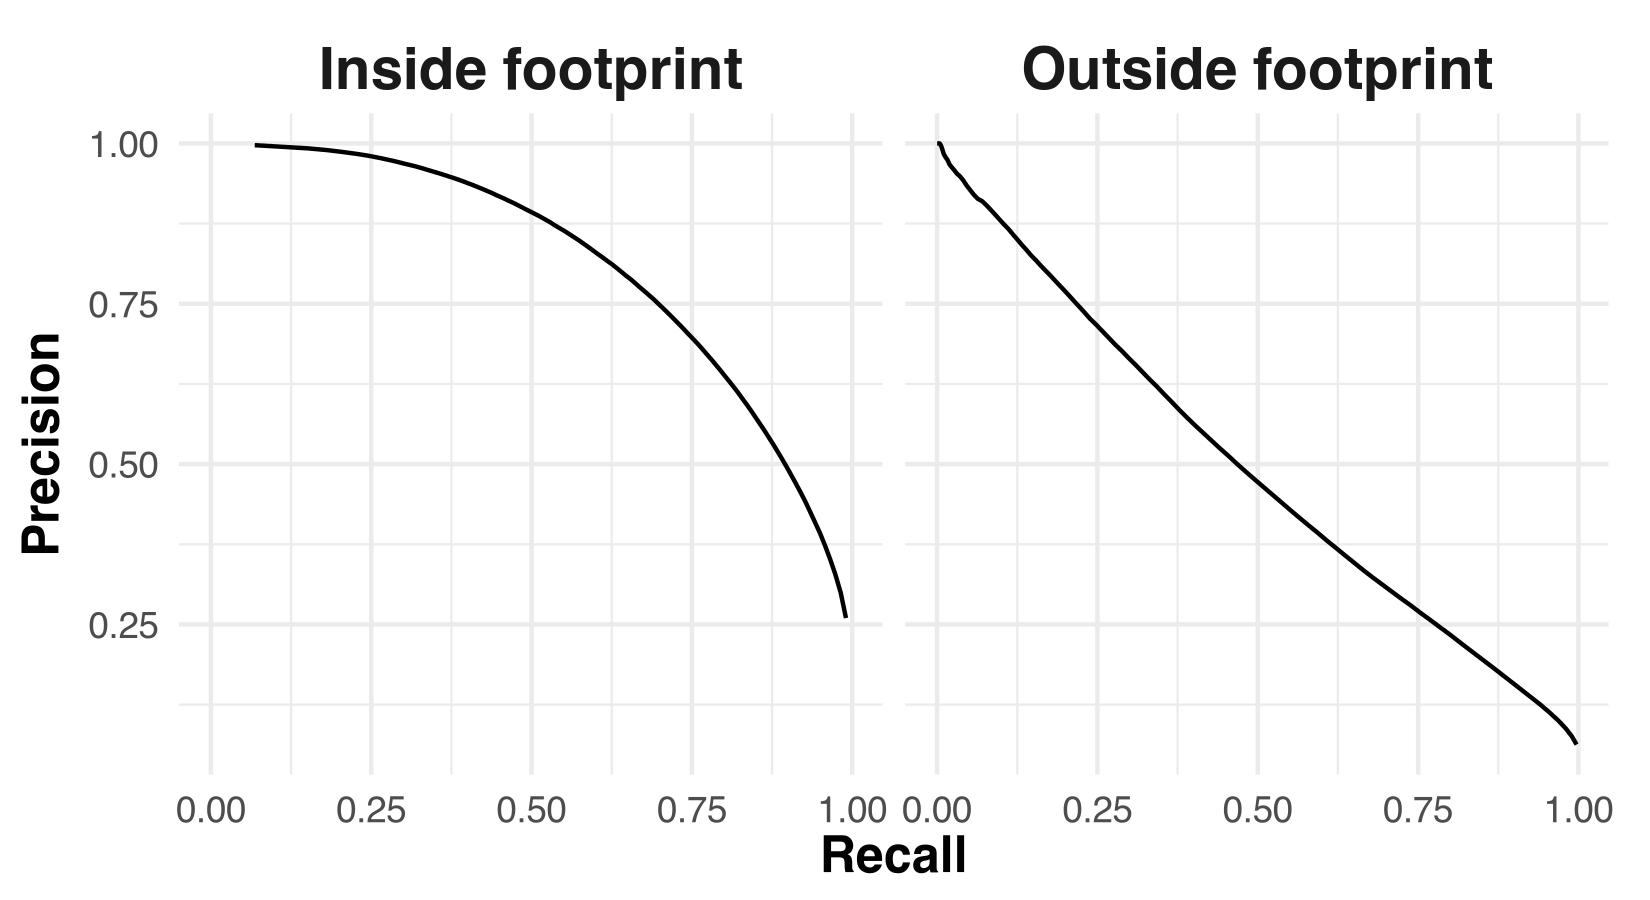
\includegraphics[width=\columnwidth]{figures/fig-pr-curves-1.png}
    \caption{Precision-recall curves of the detection presence/absence classification model, shown for both the inside S1 footprint test and simulated outside S1 footprint test.}
    \label{fig:fig-pr-curves}
\end{figure}

\begin{figure}[H]
    \centering
    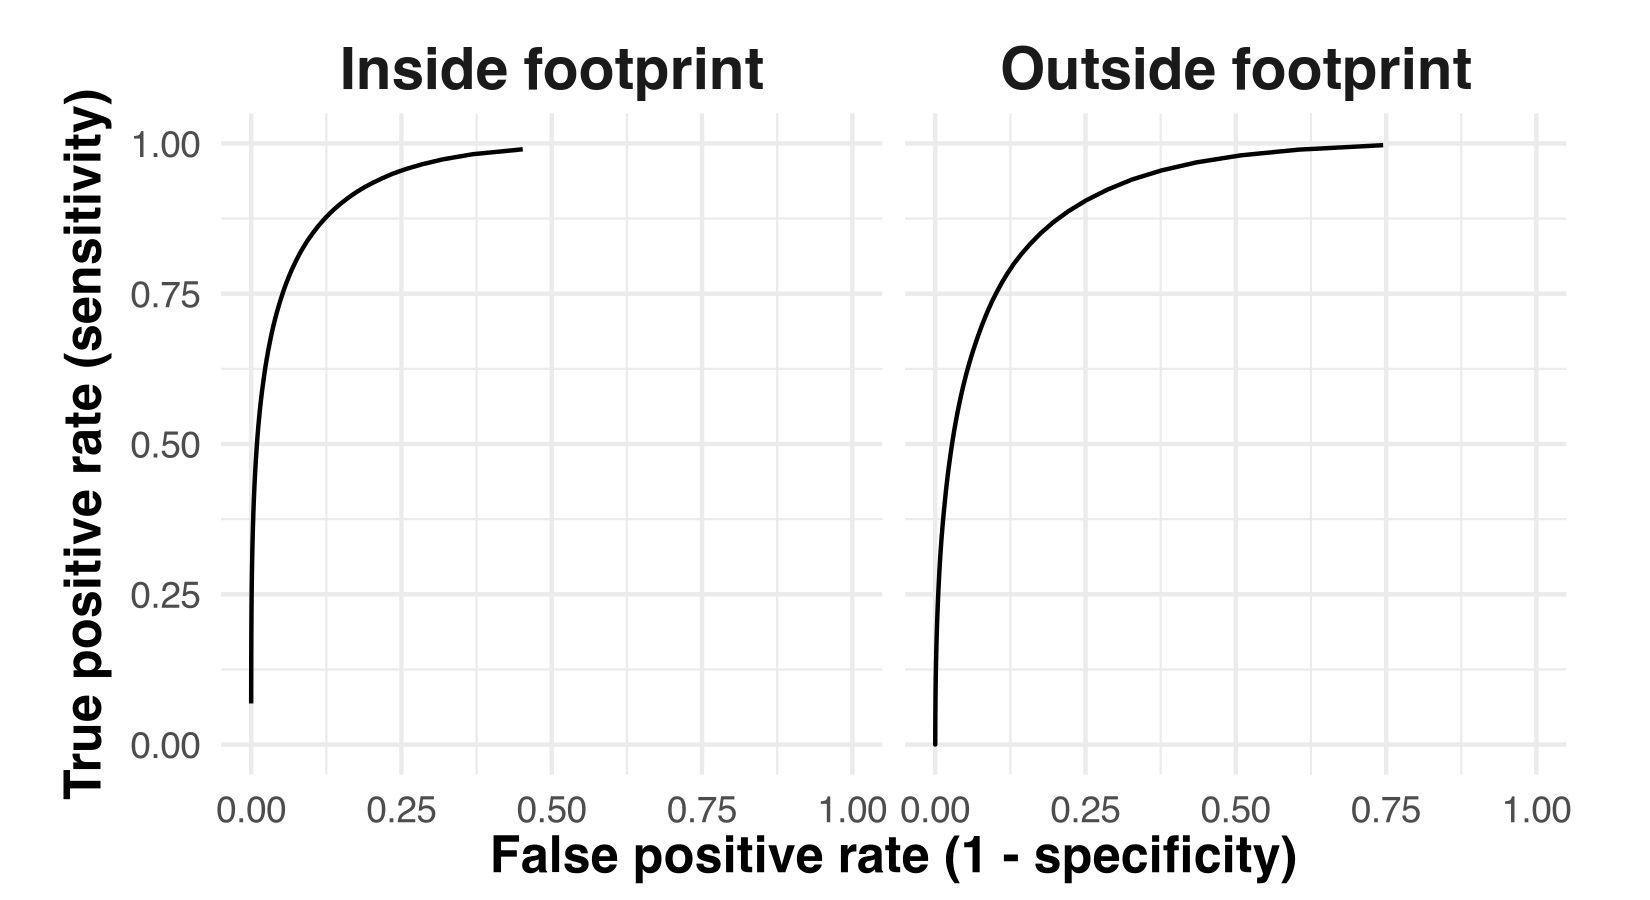
\includegraphics[width=\columnwidth]{figures/fig-roc-curves-1.png}
    \caption{Receiver Operating Characteristic (ROC) curves of the detection classification model, shown for both the inside S1 footprint test and simulated outside S1 footprint test.}
    \label{fig:fig-roc-curves}
\end{figure}

\begin{figure}[H]
    \centering
    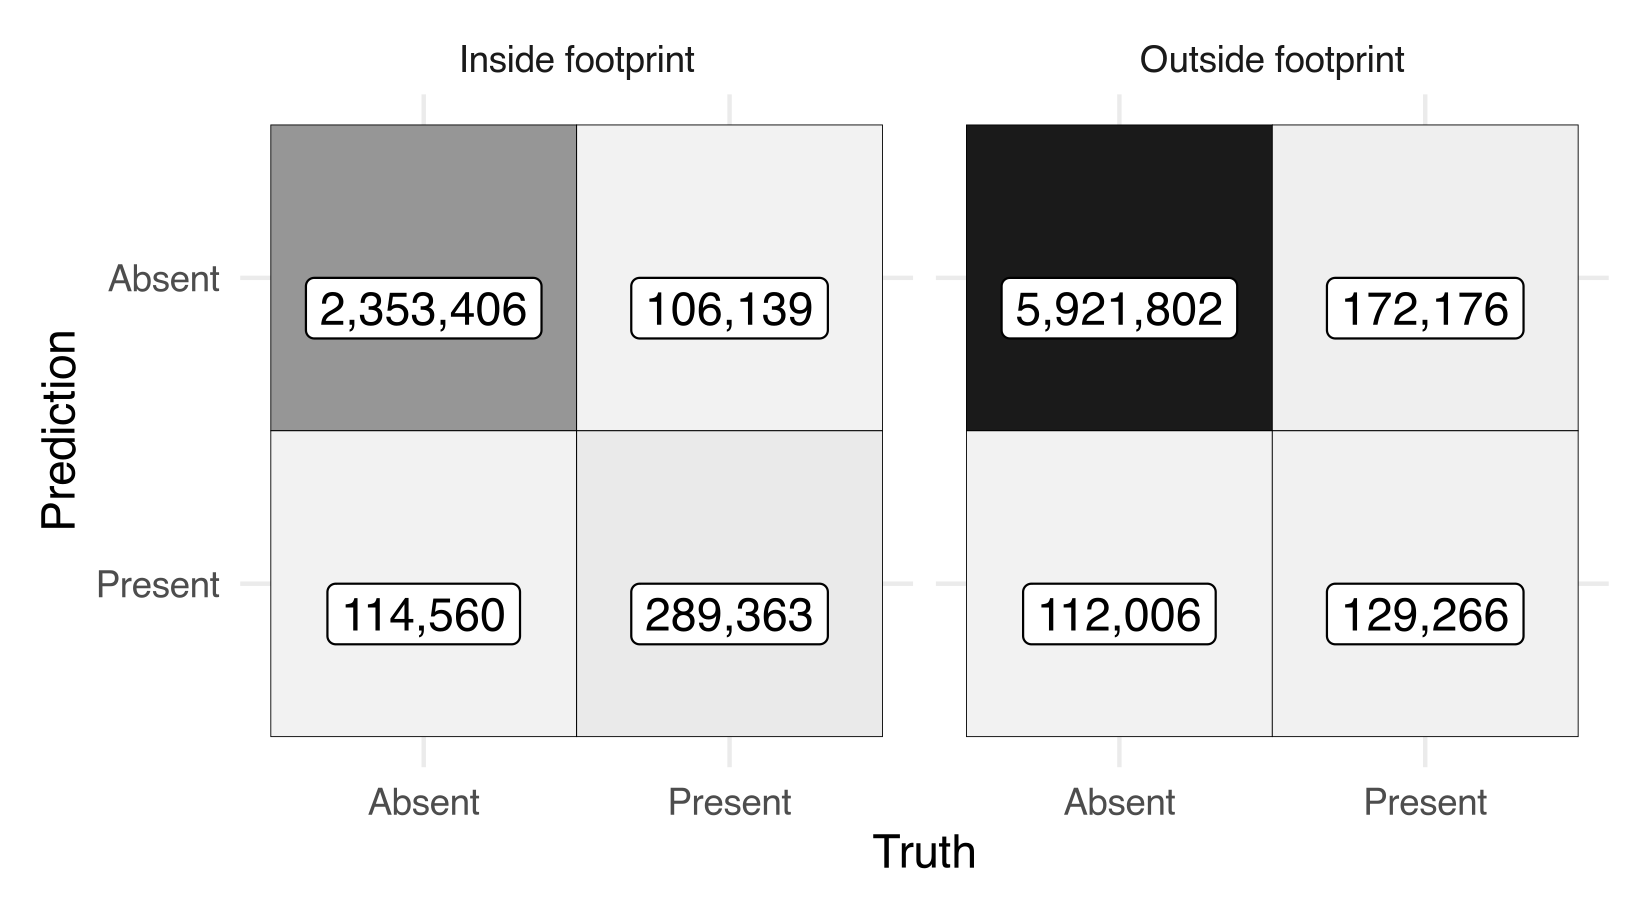
\includegraphics[width=\columnwidth]{figures/fig-conf-mat-1.png}
    \caption{Confusion matrices of the detection classification model, shown for both the inside S1 footprint test and simulated outside S1 footprint test.}
    \label{fig:fig-conf-mat}
\end{figure}


\begin{table}[!h]
\centering
\caption{\label{tab:all_performance_metrics_table}Summary of \DIFdelbeginFL \DIFdelFL{dark fleet }\DIFdelendFL \DIFaddbeginFL \DIFaddFL{S1-unmatched }\DIFaddendFL model performance metrics for the: 1) emissions regression model; 2) detections classification \DIFdelbeginFL \DIFdelFL{mode}\DIFdelendFL \DIFaddbeginFL \DIFaddFL{model}\DIFaddendFL ; and 3) detections regression model. Performance estimates for each metric are shown for both the inside S1 footprint and outside S1 footprint tests. All metrics are calculated at the unit of observation except for 'Total percent error', which is the percentage error in the total sum of all predictions relative to the total sum of all truth values.}
\centering
\fontsize{7}{9}\selectfont
\DIFdelbeginFL %DIFDELCMD < \begin{tabular}[t]{l|l|l|r|r}
%DIFDELCMD < \hline
%DIFDELCMD < Model & Pollutant & Metric & Inside footprint & Outside footprint\\
%DIFDELCMD < \hline
%DIFDELCMD < Emissions regression & CO2 & Traditional R² & 0.96 & 0.73\\
%DIFDELCMD < \hline
%DIFDELCMD < Emissions regression & CH4 & Traditional R² & 0.91 & 0.71\\
%DIFDELCMD < \hline
%DIFDELCMD < Emissions regression & N2O & Traditional R² & 0.96 & 0.74\\
%DIFDELCMD < \hline
%DIFDELCMD < Emissions regression & CO & Traditional R² & 0.92 & 0.70\\
%DIFDELCMD < \hline
%DIFDELCMD < Emissions regression & NOX & Traditional R² & 0.89 & 0.65\\
%DIFDELCMD < \hline
%DIFDELCMD < Emissions regression & SOX & Traditional R² & 0.96 & 0.74\\
%DIFDELCMD < \hline
%DIFDELCMD < Emissions regression & PM2.5 & Traditional R² & 0.96 & 0.75\\
%DIFDELCMD < \hline
%DIFDELCMD < Emissions regression & PM10 & Traditional R² & 0.96 & 0.75\\
%DIFDELCMD < \hline
%DIFDELCMD < Emissions regression & VOCs & Traditional R² & 0.95 & 0.75\\
%DIFDELCMD < \hline
%DIFDELCMD < Emissions regression & CO2 & Total percent error & -7.40 & -10.61\\
%DIFDELCMD < \hline
%DIFDELCMD < Emissions regression & CH4 & Total percent error & -12.04 & -12.74\\
%DIFDELCMD < \hline
%DIFDELCMD < Emissions regression & N2O & Total percent error & -7.18 & -8.77\\
%DIFDELCMD < \hline
%DIFDELCMD < Emissions regression & CO & Total percent error & -13.81 & -19.05\\
%DIFDELCMD < \hline
%DIFDELCMD < Emissions regression & NOX & Total percent error & -17.58 & -27.42\\
%DIFDELCMD < \hline
%DIFDELCMD < Emissions regression & SOX & Total percent error & -8.72 & -11.60\\
%DIFDELCMD < \hline
%DIFDELCMD < Emissions regression & PM2.5 & Total percent error & -7.18 & -6.28\\
%DIFDELCMD < \hline
%DIFDELCMD < Emissions regression & PM10 & Total percent error & -7.18 & -6.28\\
%DIFDELCMD < \hline
%DIFDELCMD < Emissions regression & VOCs & Total percent error & -4.02 & 3.46\\
%DIFDELCMD < \hline
%DIFDELCMD < Detections classification & - & Accuracy & 0.92 & 0.95\\
%DIFDELCMD < \hline
%DIFDELCMD < Detections classification & - & F1 score & 0.73 & 0.45\\
%DIFDELCMD < \hline
%DIFDELCMD < Detections classification & - & Precision & 0.73 & 0.47\\
%DIFDELCMD < \hline
%DIFDELCMD < Detections classification & - & Precision-recall AUC & 0.81 & 0.45\\
%DIFDELCMD < \hline
%DIFDELCMD < Detections classification & - & recall & 0.72 & 0.43\\
%DIFDELCMD < \hline
%DIFDELCMD < Detections classification & - & ROC AUC & 0.95 & 0.90\\
%DIFDELCMD < \hline
%DIFDELCMD < Detections classification & - & Sensitivity & 0.72 & 0.43\\
%DIFDELCMD < \hline
%DIFDELCMD < Detections classification & - & Specificity & 0.96 & 0.98\\
%DIFDELCMD < \hline
%DIFDELCMD < Detections regression & - & Traditional R² & 0.70 & 0.21\\
%DIFDELCMD < \hline
%DIFDELCMD < Detections regression & - & Total percent error & 1.18 & 48.50\\
%DIFDELCMD < \hline
%DIFDELCMD < \end{tabular}
%DIFDELCMD < %%%
\DIFdelendFL \DIFaddbeginFL \begin{tabular}[t]{l|l|l|r|r}
\hline
Model & Pollutant & Metric & Inside footprint & Outside footprint\\
\hline
Emissions regression & CO2 & Traditional R² & 0.94 & 0.74\\
\hline
Emissions regression & CH4 & Traditional R² & 0.91 & 0.64\\
\hline
Emissions regression & N2O & Traditional R² & 0.95 & 0.72\\
\hline
Emissions regression & CO & Traditional R² & 0.92 & 0.64\\
\hline
Emissions regression & NOX & Traditional R² & 0.87 & 0.59\\
\hline
Emissions regression & SOX & Traditional R² & 0.96 & 0.74\\
\hline
Emissions regression & PM2.5 & Traditional R² & 0.94 & 0.66\\
\hline
Emissions regression & PM10 & Traditional R² & 0.94 & 0.66\\
\hline
Emissions regression & VOCs & Traditional R² & 0.88 & 0.61\\
\hline
Emissions regression & CO2 & Total percent error & -7.76 & -9.97\\
\hline
Emissions regression & CH4 & Total percent error & -19.21 & -29.90\\
\hline
Emissions regression & N2O & Total percent error & -9.82 & -15.41\\
\hline
Emissions regression & CO & Total percent error & -18.06 & -29.18\\
\hline
Emissions regression & NOX & Total percent error & -22.54 & -36.33\\
\hline
Emissions regression & SOX & Total percent error & -5.51 & -8.02\\
\hline
Emissions regression & PM2.5 & Total percent error & -14.53 & -25.16\\
\hline
Emissions regression & PM10 & Total percent error & -14.53 & -25.16\\
\hline
Emissions regression & VOCs & Total percent error & -21.11 & -32.35\\
\hline
Detections classification & - & Accuracy & 0.92 & 0.96\\
\hline
Detections classification & - & F1 score & 0.72 & 0.48\\
\hline
Detections classification & - & Precision & 0.72 & 0.54\\
\hline
Detections classification & - & Precision-recall AUC & 0.81 & 0.50\\
\hline
Detections classification & - & Recall & 0.73 & 0.43\\
\hline
Detections classification & - & ROC AUC & 0.95 & 0.92\\
\hline
Detections classification & - & Sensitivity & 0.73 & 0.43\\
\hline
Detections classification & - & Specificity & 0.95 & 0.98\\
\hline
Detections regression & - & Traditional R² & 0.68 & 0.45\\
\hline
Detections regression & - & Total percent error & 0.31 & 16.15\\
\hline
\end{tabular}
\DIFaddendFL \end{table}
\DIFaddbegin \FloatBarrier
\DIFaddend 

\subsubsection{Feature importance}

After assessing model performance, we perform a final fit using the entire dataset to assess feature importance for the three \DIFdelbegin \DIFdel{non-broadcasting }\DIFdelend \DIFaddbegin \DIFadd{S1-unmatched }\DIFaddend emissions random forest models (Fig \ref{fig:fig-feature-importance}). Feature importance was quantified using the bias-corrected Gini index \cite{nembrini2018revival}, as implemented for random forests in the ranger R package \cite{ranger}. This metric quantifies how much each model feature reduces node impurity when it is used to make splits in the random forest's decision trees.

\begin{figure}[!p]
    \centering
    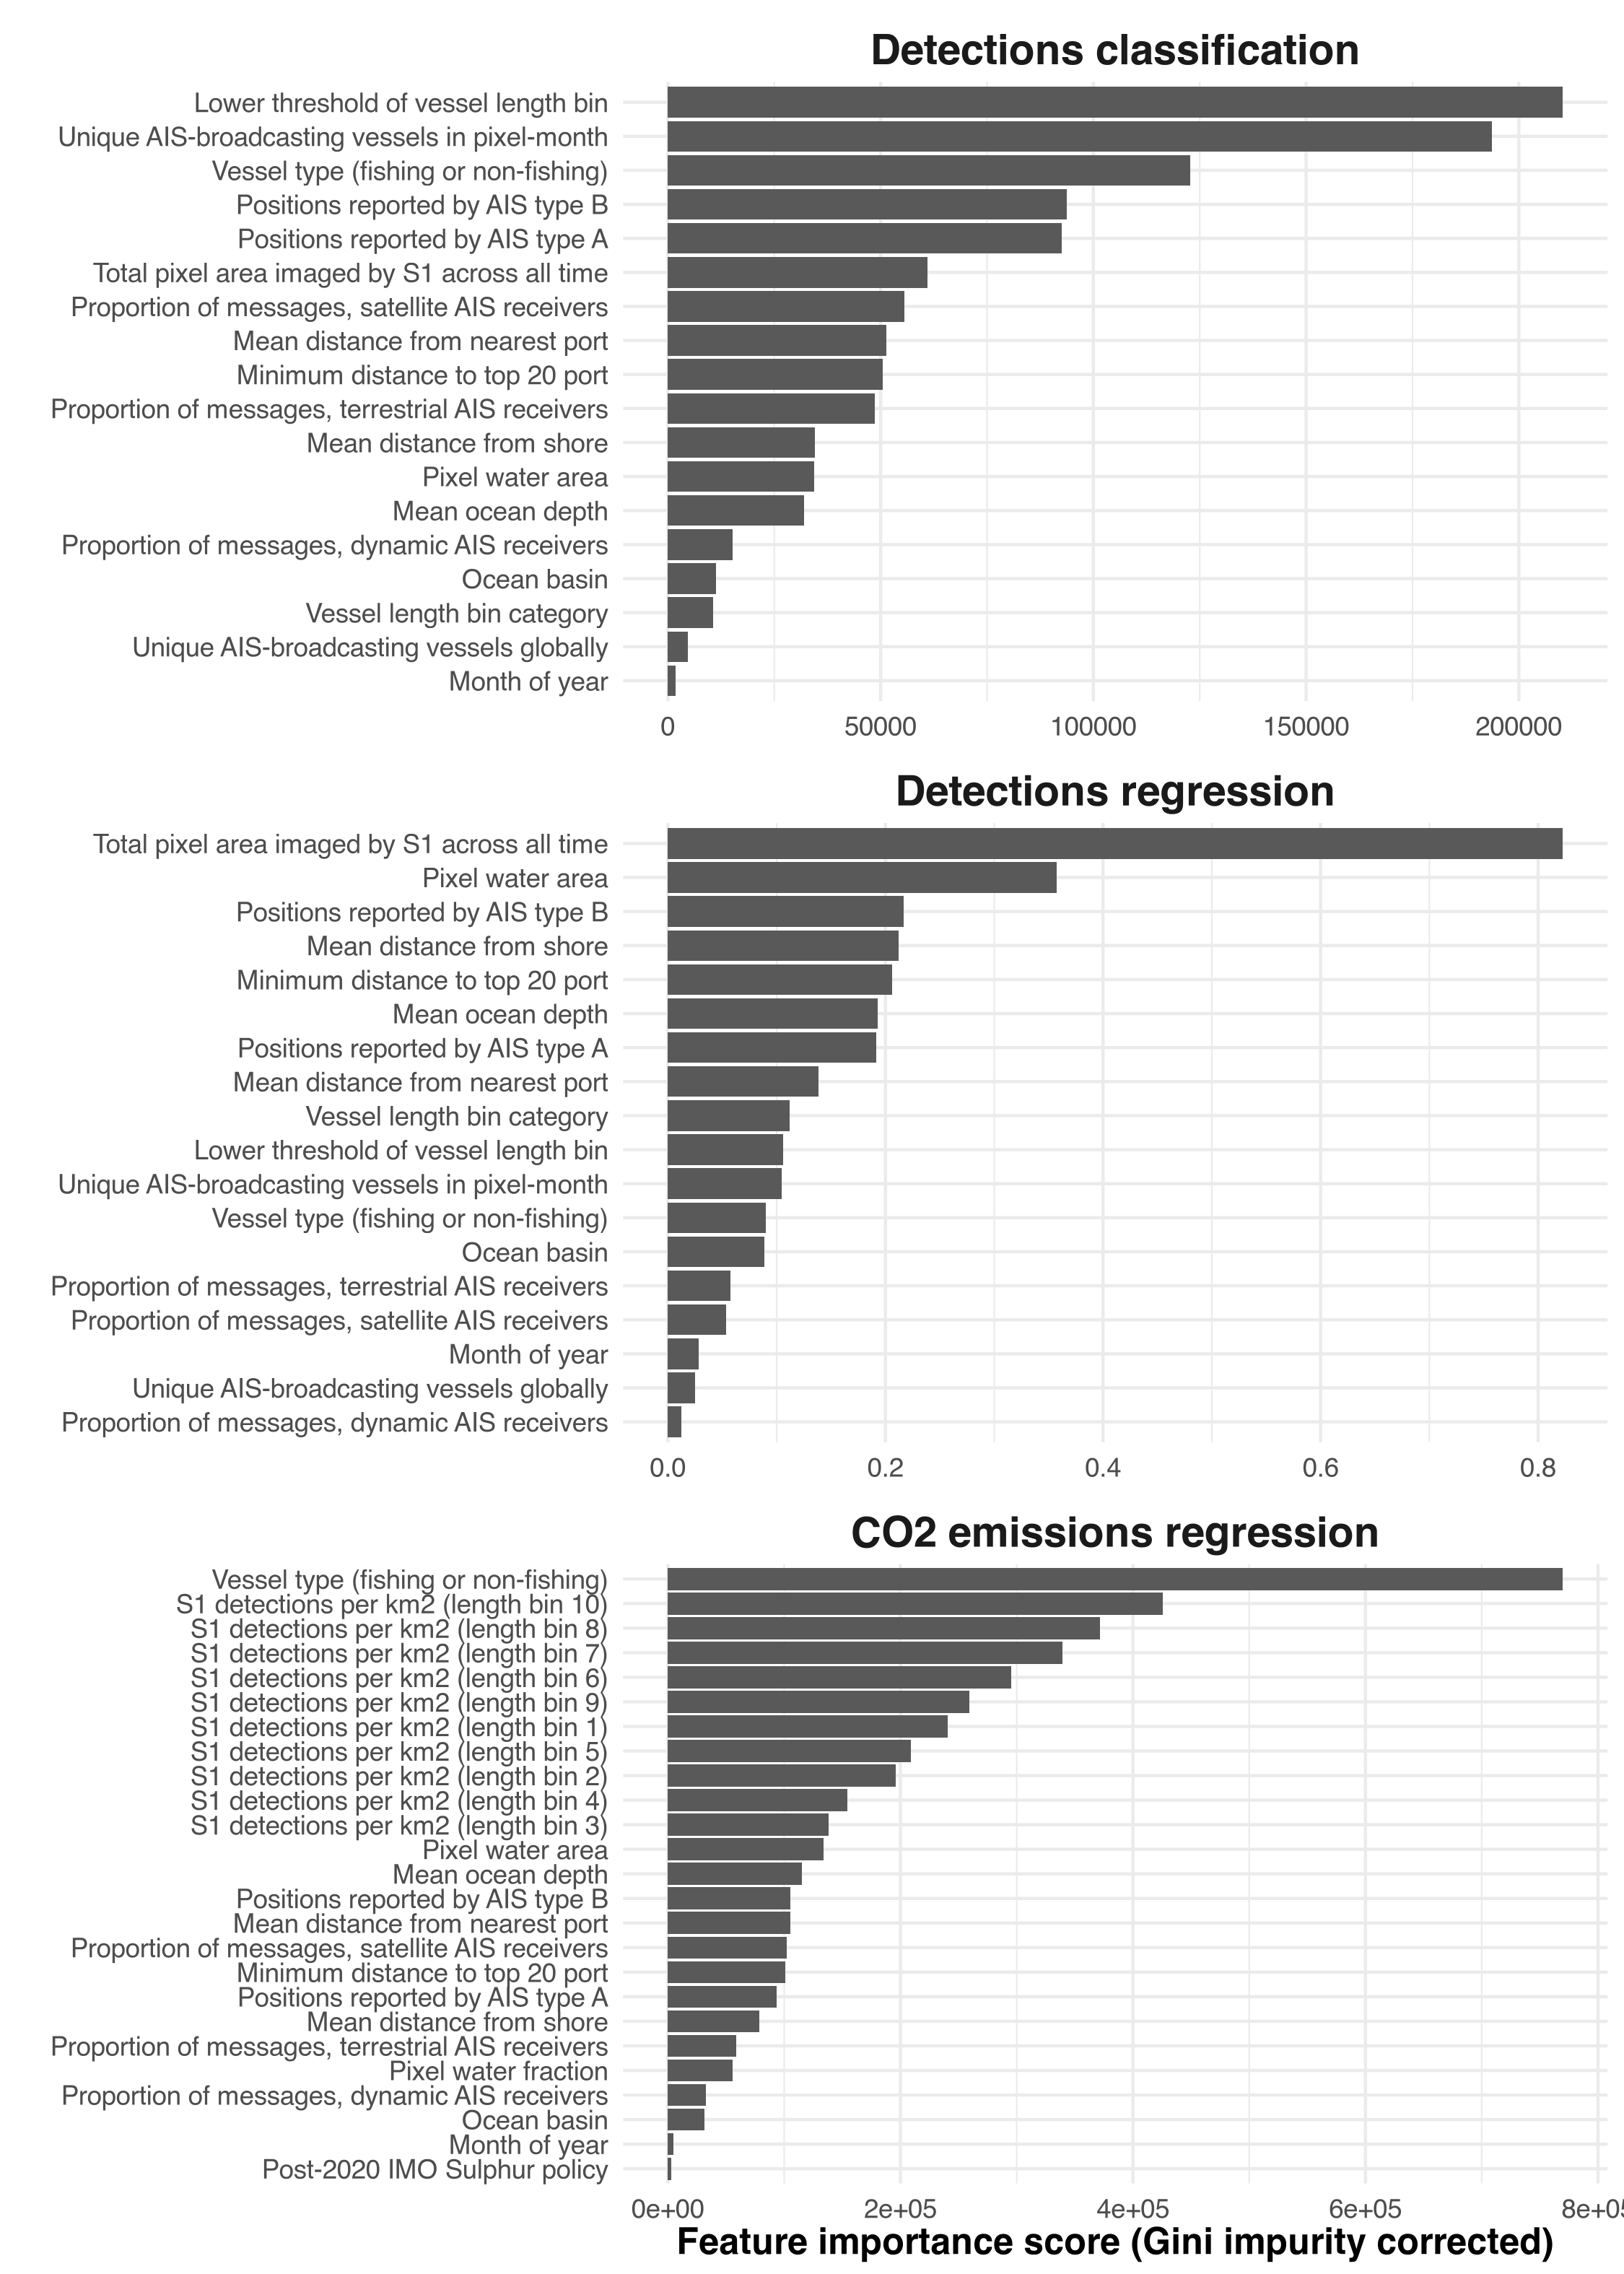
\includegraphics[width=\columnwidth]{figures/fig-feature-importance-1.png}
    \caption{Feature importance \DIFdelbeginFL \DIFdelFL{plots }\DIFdelendFL for \DIFdelbeginFL \DIFdelFL{the: 1}\DIFdelendFL \DIFaddbeginFL \DIFaddFL{(a}\DIFaddendFL ) \DIFaddbeginFL \DIFaddFL{the }\DIFaddendFL detections (presence/absence) classification model\DIFdelbeginFL \DIFdelFL{;
2}\DIFdelendFL \DIFaddbeginFL \DIFaddFL{, (b}\DIFaddendFL ) \DIFaddbeginFL \DIFaddFL{the }\DIFaddendFL detections regression model\DIFdelbeginFL \DIFdelFL{; }\DIFdelendFL \DIFaddbeginFL \DIFaddFL{, }\DIFaddendFL and \DIFdelbeginFL \DIFdelFL{3}\DIFdelendFL \DIFaddbeginFL \DIFaddFL{(c}\DIFaddendFL ) \DIFaddbeginFL \DIFaddFL{the }\DIFaddendFL CO$_2$ emissions regression model.}
    \label{fig:fig-feature-importance}
\end{figure}

\subsubsection{Linear regression fit statistics for \DIFdelbegin \DIFdel{non-gas models}\DIFdelend \DIFaddbegin \DIFadd{other pollutants}\DIFaddend }

Here we look at the linear regression fit statistics for the final models to convert CO$_2$ emissions to emissions of non-CO$_2$ gases (other GHGs and non-GHG pollutants), trained using the full dataset (Table \ref{tab:lm_other_gases_tidy_fit_stats}).

\begin{table}[!h]
\centering
\caption{\label{tab:lm_other_gases_tidy_fit_stats}Linear regression fit statistics for the final models trained to estimate emissions of non-CO$_2$ gases from CO$_2$ emissions. The model for each gas \DIFdelbeginFL \DIFdelFL{has 2 fit }\DIFdelendFL \DIFaddbeginFL \DIFaddFL{is a zero-intercept linear regression with 5 }\DIFaddendFL terms\DIFaddbeginFL \DIFaddFL{: CO$_2$ emissions interacted with each combination of period (pre/post-2020 IMO sulfur policy) and vessel type (fishing/non-fishing), plus CO$_2$ emissions interacted with the log of mean distance from shore}\DIFaddendFL .}
\centering
\fontsize{7}{9}\selectfont
\DIFdelbeginFL %DIFDELCMD < \begin{tabular}[t]{l|l|r|l|r|r}
%DIFDELCMD < \hline
%DIFDELCMD < Pollutant & Term & Coefficient estimate & Standard error & T-statistic & p.value\\
%DIFDELCMD < \hline
%DIFDELCMD < CH4 & emissionsco2mt:post2020FALSE & 0.000 & 8.65e-09 & 1993.619 & 0\\
%DIFDELCMD < \hline
%DIFDELCMD < CH4 & emissionsco2mt:post2020TRUE & 0.000 & 6.16e-09 & 2857.130 & 0\\
%DIFDELCMD < \hline
%DIFDELCMD < N2O & emissionsco2mt:post2020FALSE & 0.000 & 3.49e-09 & 14253.703 & 0\\
%DIFDELCMD < \hline
%DIFDELCMD < N2O & emissionsco2mt:post2020TRUE & 0.000 & 2.48e-09 & 20123.201 & 0\\
%DIFDELCMD < \hline
%DIFDELCMD < CO & emissionsco2mt:post2020FALSE & 0.001 & 3.35e-07 & 2455.044 & 0\\
%DIFDELCMD < \hline
%DIFDELCMD < CO & emissionsco2mt:post2020TRUE & 0.001 & 2.38e-07 & 3471.338 & 0\\
%DIFDELCMD < \hline
%DIFDELCMD < NOX & emissionsco2mt:post2020FALSE & 0.017 & 8.33e-06 & 2026.457 & 0\\
%DIFDELCMD < \hline
%DIFDELCMD < NOX & emissionsco2mt:post2020TRUE & 0.017 & 5.93e-06 & 2826.873 & 0\\
%DIFDELCMD < \hline
%DIFDELCMD < SOX & emissionsco2mt:post2020FALSE & 0.006 & 3.63e-08 & 170143.414 & 0\\
%DIFDELCMD < \hline
%DIFDELCMD < SOX & emissionsco2mt:post2020TRUE & 0.001 & 2.59e-08 & 47783.674 & 0\\
%DIFDELCMD < \hline
%DIFDELCMD < PM2.5 & emissionsco2mt:post2020FALSE & 0.002 & 1.13e-07 & 15453.046 & 0\\
%DIFDELCMD < \hline
%DIFDELCMD < PM2.5 & emissionsco2mt:post2020TRUE & 0.000 & 8.06e-08 & 4512.650 & 0\\
%DIFDELCMD < \hline
%DIFDELCMD < PM10 & emissionsco2mt:post2020FALSE & 0.002 & 1.23e-07 & 15453.046 & 0\\
%DIFDELCMD < \hline
%DIFDELCMD < PM10 & emissionsco2mt:post2020TRUE & 0.000 & 8.76e-08 & 4512.650 & 0\\
%DIFDELCMD < \hline
%DIFDELCMD < VOCs & emissionsco2mt:post2020FALSE & 0.001 & 3.57e-07 & 3405.442 & 0\\
%DIFDELCMD < \hline
%DIFDELCMD < VOCs & emissionsco2mt:post2020TRUE & 0.001 & 2.54e-07 & 4902.133 & 0\\
%DIFDELCMD < \hline
%DIFDELCMD < \end{tabular}
%DIFDELCMD < %%%
\DIFdelendFL \DIFaddbeginFL \begin{tabular}[t]{l|l|l|l|r|l}
\hline
Pollutant & Term & Estimate & SE & T-stat. & p-value\\
\hline
CH4 & CO2 : log(distance from shore + 1) & 1.25e-06 & 3.29e-09 & 380.0 & $<$0.001\\
\hline
CH4 & CO2 : pre-2020 : non-fishing & -1.21e-06 & 3.17e-08 & -38.1 & $<$0.001\\
\hline
CH4 & CO2 : pre-2020 : fishing & 3.69e-06 & 8.41e-08 & 43.9 & $<$0.001\\
\hline
CH4 & CO2 : post-2020 : non-fishing & -1.92e-06 & 3.14e-08 & -61.4 & $<$0.001\\
\hline
CH4 & CO2 : post-2020 : fishing & 3.73e-06 & 4.52e-08 & 82.7 & $<$0.001\\
\hline
N2O & CO2 : log(distance from shore + 1) & 7.13e-07 & 2.32e-09 & 308.1 & $<$0.001\\
\hline
N2O & CO2 : pre-2020 : non-fishing & 4.17e-05 & 2.23e-08 & 1870.0 & $<$0.001\\
\hline
N2O & CO2 : pre-2020 : fishing & 4.30e-05 & 5.92e-08 & 727.2 & $<$0.001\\
\hline
N2O & CO2 : post-2020 : non-fishing & 4.12e-05 & 2.20e-08 & 1866.4 & $<$0.001\\
\hline
N2O & CO2 : post-2020 : fishing & 4.39e-05 & 3.18e-08 & 1380.3 & $<$0.001\\
\hline
CO & CO2 : log(distance from shore + 1) & 6.02e-05 & 1.57e-07 & 382.4 & $<$0.001\\
\hline
CO & CO2 : pre-2020 : non-fishing & 2.91e-05 & 1.51e-06 & 19.2 & $<$0.001\\
\hline
CO & CO2 : pre-2020 : fishing & 2.73e-04 & 4.02e-06 & 67.9 & $<$0.001\\
\hline
CO & CO2 : post-2020 : non-fishing & -5.48e-06 & 1.50e-06 & -3.7 & $<$0.001\\
\hline
CO & CO2 : post-2020 : fishing & 2.76e-04 & 2.16e-06 & 128.1 & $<$0.001\\
\hline
NOX & CO2 : log(distance from shore + 1) & 2.02e-03 & 4.33e-06 & 466.8 & $<$0.001\\
\hline
NOX & CO2 : pre-2020 : non-fishing & -7.34e-03 & 4.16e-05 & -176.3 & $<$0.001\\
\hline
NOX & CO2 : pre-2020 : fishing & -9.75e-04 & 1.10e-04 & -8.8 & $<$0.001\\
\hline
NOX & CO2 : post-2020 : non-fishing & -8.45e-03 & 4.12e-05 & -205.3 & $<$0.001\\
\hline
NOX & CO2 : post-2020 : fishing & -2.14e-03 & 5.93e-05 & -36.1 & $<$0.001\\
\hline
SOX & CO2 : log(distance from shore + 1) & -1.24e-05 & 7.15e-08 & -173.1 & $<$0.001\\
\hline
SOX & CO2 : pre-2020 : non-fishing & 6.30e-03 & 6.88e-07 & 9167.7 & $<$0.001\\
\hline
SOX & CO2 : pre-2020 : fishing & 6.37e-03 & 1.83e-06 & 3487.2 & $<$0.001\\
\hline
SOX & CO2 : post-2020 : non-fishing & 1.66e-03 & 6.81e-07 & 2442.1 & $<$0.001\\
\hline
SOX & CO2 : post-2020 : fishing & 1.67e-03 & 9.81e-07 & 1706.2 & $<$0.001\\
\hline
PM2.5 & CO2 : log(distance from shore + 1) & 3.65e-05 & 9.11e-08 & 401.1 & $<$0.001\\
\hline
PM2.5 & CO2 : pre-2020 : non-fishing & 4.14e-04 & 8.76e-07 & 472.7 & $<$0.001\\
\hline
PM2.5 & CO2 : pre-2020 : fishing & 5.33e-04 & 2.33e-06 & 229.0 & $<$0.001\\
\hline
PM2.5 & CO2 : post-2020 : non-fishing & 5.04e-05 & 8.67e-07 & 58.2 & $<$0.001\\
\hline
PM2.5 & CO2 : post-2020 : fishing & 2.10e-04 & 1.25e-06 & 168.4 & $<$0.001\\
\hline
PM10 & CO2 : log(distance from shore + 1) & 3.97e-05 & 9.90e-08 & 401.1 & $<$0.001\\
\hline
PM10 & CO2 : pre-2020 : non-fishing & 4.50e-04 & 9.52e-07 & 472.7 & $<$0.001\\
\hline
PM10 & CO2 : pre-2020 : fishing & 5.79e-04 & 2.53e-06 & 229.0 & $<$0.001\\
\hline
PM10 & CO2 : post-2020 : non-fishing & 5.48e-05 & 9.42e-07 & 58.2 & $<$0.001\\
\hline
PM10 & CO2 : post-2020 : fishing & 2.29e-04 & 1.36e-06 & 168.4 & $<$0.001\\
\hline
VOCs & CO2 : log(distance from shore + 1) & 1.00e-04 & 2.02e-07 & 495.8 & $<$0.001\\
\hline
VOCs & CO2 : pre-2020 : non-fishing & -3.94e-04 & 1.94e-06 & -203.1 & $<$0.001\\
\hline
VOCs & CO2 : pre-2020 : fishing & -2.01e-04 & 5.15e-06 & -39.1 & $<$0.001\\
\hline
VOCs & CO2 : post-2020 : non-fishing & -4.38e-04 & 1.92e-06 & -228.1 & $<$0.001\\
\hline
VOCs & CO2 : post-2020 : fishing & -2.10e-04 & 2.77e-06 & -75.7 & $<$0.001\\
\hline
\end{tabular}
\DIFaddendFL \end{table}
\DIFaddbegin \FloatBarrier
\DIFaddend 

\subsubsection{Predicting \DIFdelbegin \DIFdel{non-broadcasting }\DIFdelend \DIFaddbegin \DIFadd{S1-unmatched }\DIFaddend emissions}

To generate the final global estimates of \DIFdelbegin \DIFdel{non-broadcasting vessel }\DIFdelend \DIFaddbegin \DIFadd{S1-unmatched }\DIFaddend emissions, we: 1) train all models (the three random forests and eight linear regressions) using the entire dataset of observations that have both S1 detections and AIS emissions (Fig \ref{fig:fig-feature-importance}, Table \ref{tab:lm_other_gases_tidy_fit_stats}; noting that again for the presence/absence detection classification model, we use a random stratified training/validation split to first calibrate the classification threshold before fitting the final model on all the data); 2) \DIFdelbegin \DIFdel{then applied }\DIFdelend \DIFaddbegin \DIFadd{apply }\DIFaddend the final trained models across all ocean pixels on a monthly basis for the entire \DIFdelbegin \DIFdel{2017-2024 }\DIFdelend \DIFaddbegin \DIFadd{2017-2025 }\DIFaddend study period. The prediction workflow followed a hierarchical logic based on \DIFdelbegin \DIFdel{the availability of }\DIFdelend \DIFaddbegin \DIFadd{whether a pixel-month was imaged by }\DIFaddend S1\DIFdelbegin \DIFdel{detections}\DIFdelend :

1. Direct estimation: If \DIFdelbegin \DIFdel{unmatched S1 detections are available for }\DIFdelend a given pixel-month \DIFaddbegin \DIFadd{was imaged by S1}\DIFaddend , we use \DIFdelbegin \DIFdel{the }\DIFdelend \DIFaddbegin \DIFadd{its observed }\DIFaddend unmatched detection density to directly predict \DIFdelbegin \DIFdel{non-broadcasting }\DIFdelend \DIFaddbegin \DIFadd{S1-unmatched }\DIFaddend CO$_2$ emissions using the emissions regression model. \DIFaddbegin \DIFadd{Pixel-months that S1 imaged but in which it made no unmatched detections in any length bin are assigned zero S1-unmatched emissions: S1 observed no unmatched vessels there, and the emissions regression, which predicts log emissions and is trained only on pixel-months with at least one matched detection, would otherwise extrapolate to a spurious positive estimate. }\DIFaddend We then use the other eight gas-specific linear regression models to convert CO$_2$ emissions to emissions of each of the other eight gases.
2. Indirect estimation: If \DIFdelbegin \DIFdel{unmatched S1 detections are not available for }\DIFdelend a given pixel-month \DIFaddbegin \DIFadd{was not imaged by S1}\DIFaddend , we: a) predict whether or not unmatched detections are present using the classification first stage of the hurdle model; then b) if unmatched detections are predicted to be present, we predict the density of unmatched detections using the regression second stage of the hurdle model; then c) we use the predicted density of unmatched detections in the emissions regression model to predict CO$_2$ emissions; and finally d) we then use the other eight gas-specific linear regression models to convert CO$_2$ emissions to emissions of each of the other eight gases. 

The final output provides a continuous global dataset of monthly \DIFdelbegin \DIFdel{non-broadcasting }\DIFdelend \DIFaddbegin \DIFadd{S1-unmatched }\DIFaddend emissions, for all three GHGs and six pollutants, from 2017 to \DIFdelbegin \DIFdel{2024 }\DIFdelend \DIFaddbegin \DIFadd{2025 }\DIFaddend at 1×1-degree resolution, disaggregated by fishing and non-fishing vessel types.

\paragraph{Direct estimation}

For this prediction, we replaced the matched S1 detection density features for each length bin used during model training with the observed unmatched S1 detection density for each of the length bin features and separately for non-fishing/fishing vessel types. We were able to use this direct estimation approach for \DIFdelbegin \DIFdel{95.3}\DIFdelend \DIFaddbegin \DIFadd{95.7}\DIFaddend \% of the total estimated \DIFdelbegin \DIFdel{non-broadcasting }\DIFdelend \DIFaddbegin \DIFadd{S1-unmatched }\DIFaddend CO$_2$ emissions (Fig. \ref{fig:fig-spatial-coverage-footprint}). This approach predicts \DIFdelbegin \DIFdel{non-broadcasting }\DIFdelend \DIFaddbegin \DIFadd{S1-unmatched }\DIFaddend emissions fully within the S1 footprint, and thus also represents the models with the highest predictive performance (Table \ref{tab:all_performance_metrics_table}).

\begin{figure}[H]
    \centering
    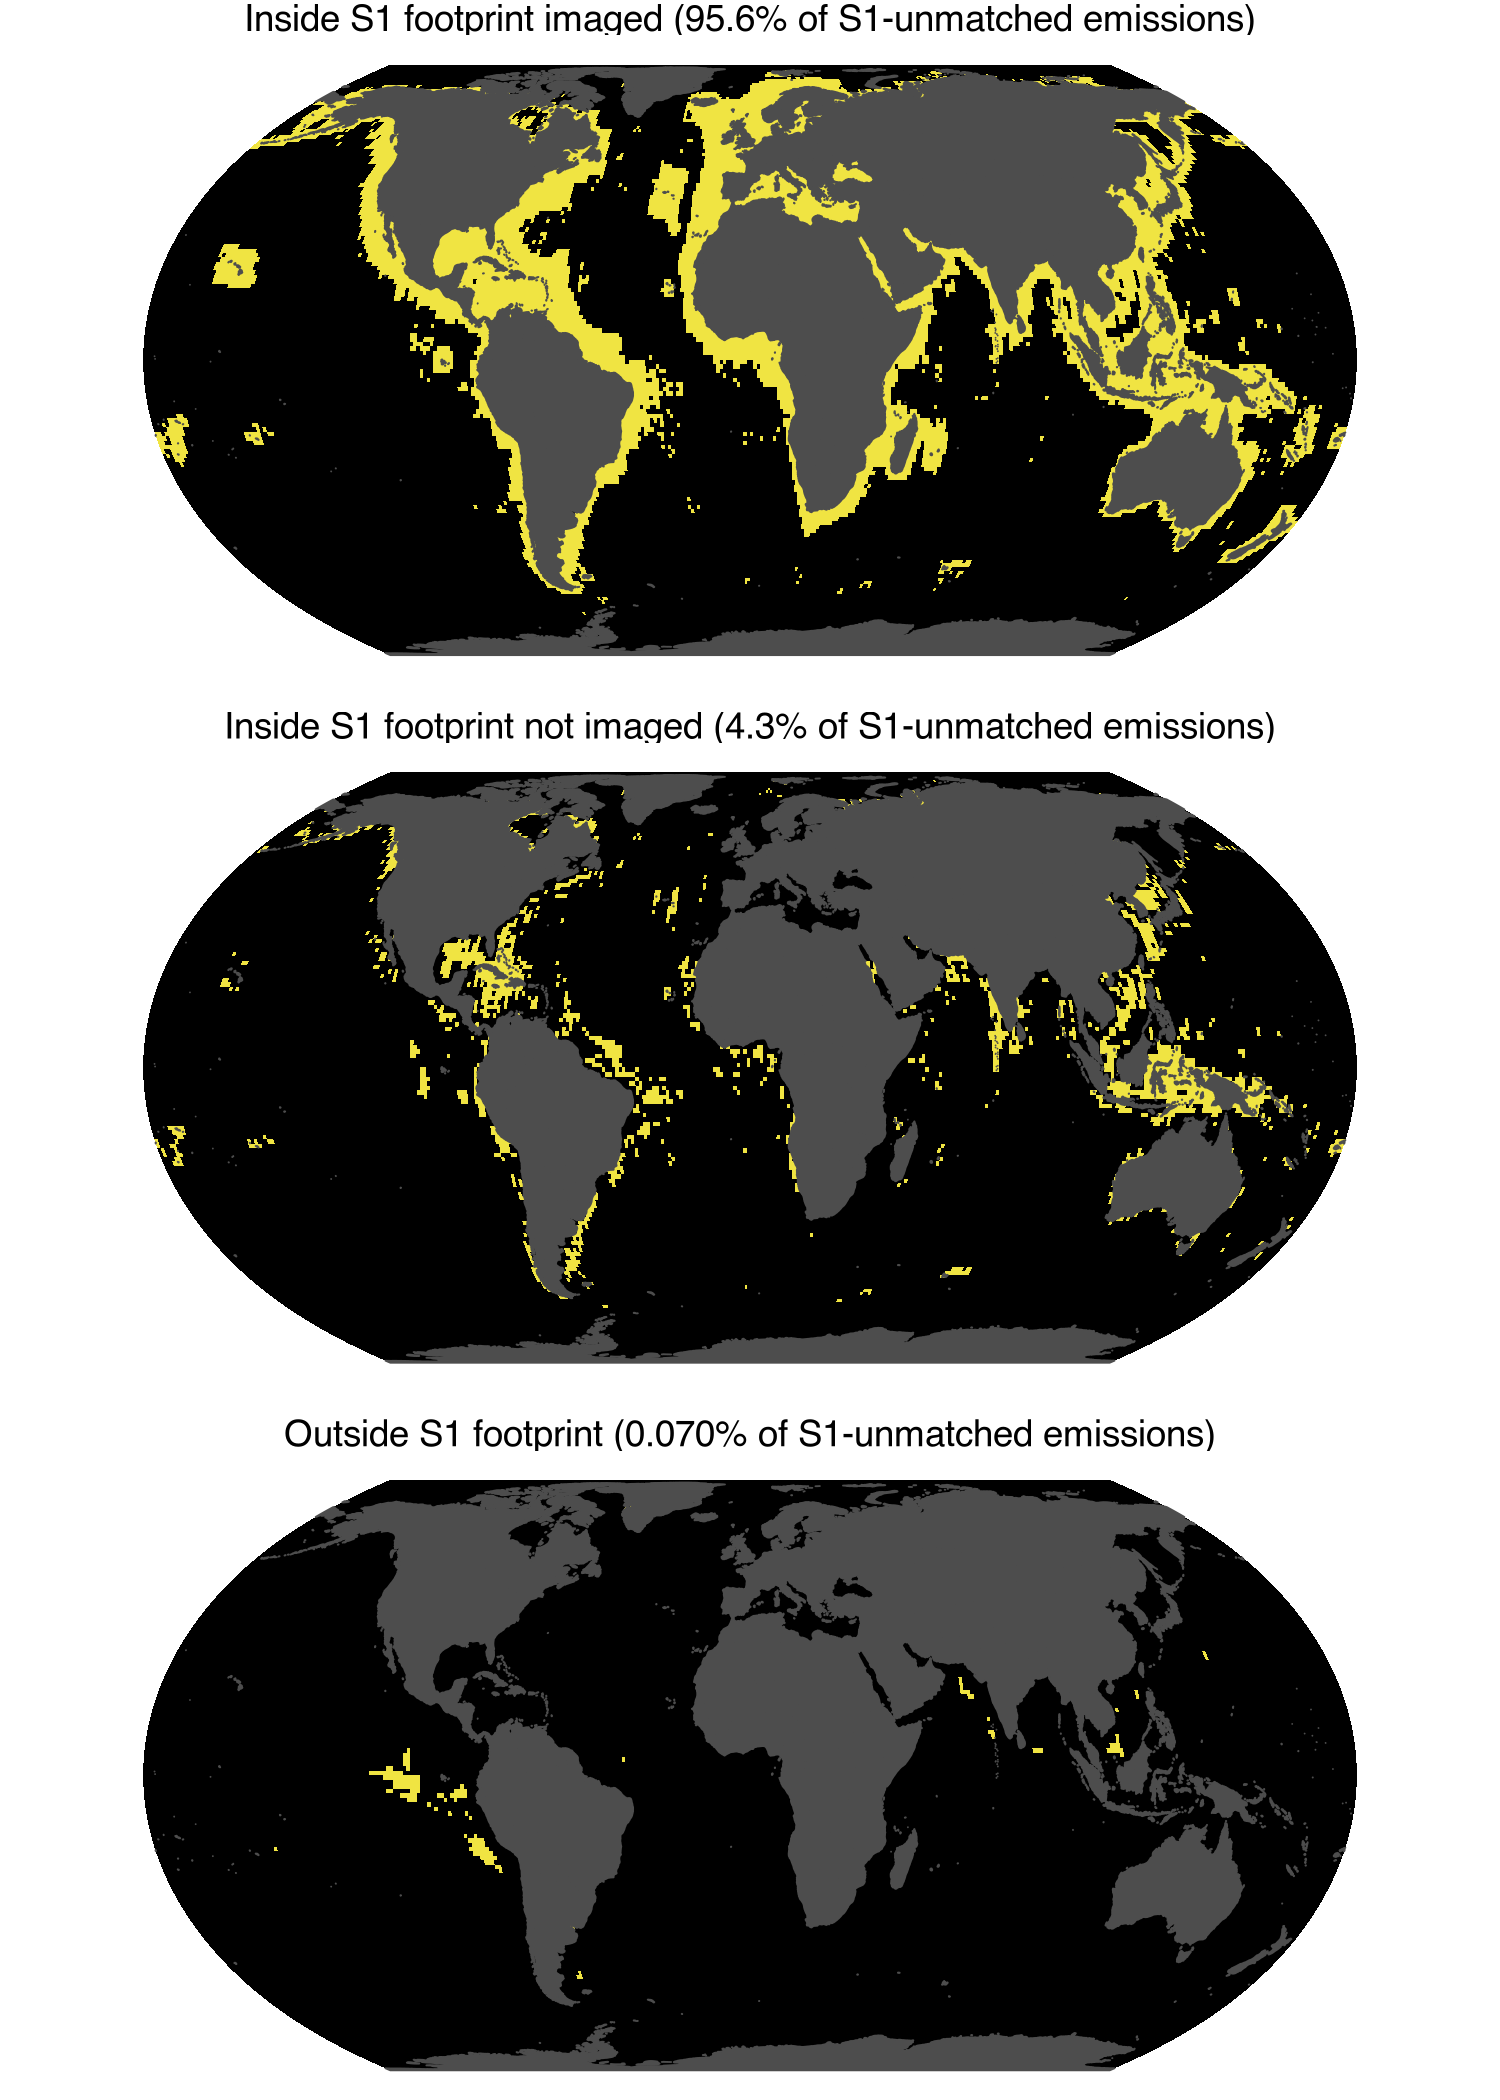
\includegraphics[width=0.8\columnwidth]{figures/fig-spatial-coverage-footprint-1.png}
    \caption{Spatial coverage of the \DIFdelbeginFL \DIFdelFL{non-broadcasting }\DIFdelendFL \DIFaddbeginFL \DIFaddFL{S1-unmatched }\DIFaddendFL emissions model. Areas are categorized according to whether they fall inside or outside the S1 footprint and whether they have been imaged by S1 at any point in time. A given pixel may be imaged in some months but not in others. Pixels outside the footprint have never been imaged. The percentage of total \DIFaddbeginFL \DIFaddFL{S1-unmatched }\DIFaddendFL CO$_{2}$ emissions \DIFdelbeginFL \DIFdelFL{from non-broadcasting vessels }\DIFdelendFL attributed to each category is shown.}
    \label{fig:fig-spatial-coverage-footprint}
\end{figure}

\paragraph{Indirect estimation}

For pixel-months where S1 detections were unavailable, either because they were not imaged due to spatiotemporal satellite heterogeneity or because they fall fully outside the S1 footprint, we first used the detections classification model to predict whether detections were present or absent for each of the length bins and fishing/non-fishing vessel types. If detections were predicted, the subsequent detection regression model was used to predict the \DIFdelbegin \DIFdel{number }\DIFdelend \DIFaddbegin \DIFadd{density }\DIFaddend of unmatched S1 detections per \DIFdelbegin \DIFdel{km}\DIFdelend \DIFaddbegin \DIFadd{unit of S1 sampling effort }\DIFaddend for each length bin and fishing/non-fishing vessel type. These predicted unmatched detection densities were then fed into the emissions regression model as the separate length-bin-related model features (for each fishing/non-fishing vessel type) to predict the resulting emissions. We \DIFdelbegin \DIFdel{do this for all nine emissions regression models corresponding to the three GHGs and six pollutants}\DIFdelend \DIFaddbegin \DIFadd{then convert the predicted CO$_2$ emissions to emissions of the other eight gases using the linear regressions described above}\DIFaddend . Of the total predicted \DIFdelbegin \DIFdel{non-broadcasting }\DIFdelend \DIFaddbegin \DIFadd{S1-unmatched }\DIFaddend CO$_2$ emissions, \DIFdelbegin \DIFdel{4.6}\DIFdelend \DIFaddbegin \DIFadd{4.2}\DIFaddend \% corresponded to indirect estimations within the S1 footprint, while only \DIFdelbegin \DIFdel{0.1}\DIFdelend \DIFaddbegin \DIFadd{0.070}\DIFaddend \% occurred entirely outside the footprint (Fig. \ref{fig:fig-spatial-coverage-footprint}).



%DIF > %%%%%%%%%%%%%%% DATA AND CODE AVAILABILITY %%%%%%%%%%%%%%%
%DIF >  Nature Communications requires both sections immediately below Methods.
\DIFaddbegin 

\section*{\DIFadd{Data availability}}

\DIFadd{All data necessary for reproducing the figures, tables and statistics in this analysis will be made available in a public GitHub repository (paper-ocean-ghg) with an accompanying Zenodo repository and DOI. It will also be made available in a Code Ocean repository with an accompanying DOI. These data include the aggregated outputs of our AIS-based and S1-unmatched emissions models, and the published inventories and validation data we compare them with. To maximize their use by future researchers and decision makers, we will also release two datasets on the Global Fishing Watch data download portal: monthly AIS-based emissions at 0.1x0.1-degree resolution by flag and vessel type, with emissions of each of the three GHGs and six pollutants, fuel consumption, hours of activity and distance traveled; and monthly S1-unmatched emissions at 1x1-degree resolution for fishing and non-fishing vessels, with emissions of each of the three GHGs and six pollutants. S\&P Global Market Intelligence's Ships Dataset, which we used under license to train the vessel characteristics models and for the registered data validation, is proprietary and available from S\&P Global. This section will be updated to include the hyperlinks and DOIs upon manuscript acceptance.
}

\section*{\DIFadd{Code availability}}

\DIFadd{All code necessary for reproducing the figures, and the tables and statistics based on our emissions estimates, from these data will be made available in the same GitHub, Zenodo and Code Ocean repositories. The emissions estimates themselves are produced by two upstream models, whose code will also be made public on GitHub upon manuscript acceptance: the AIS-based emissions model (ocean-ghg repository), which requires authenticated access to Global Fishing Watch data on Google BigQuery to run, and the S1-unmatched emissions models (s1\_ratios\_rf repository), which require the same access and extensive high-performance computing. Their outputs are included in the paper-ocean-ghg repository, so reproducing our results requires neither BigQuery access nor high-performance computing. The vessel characteristics models (Tables \ref{tab:model-summary} and \ref{tab:characteristic-availability}) were developed by Global Fishing Watch, and their predictions enter the AIS-based emissions model as inputs. This section will be updated to include the hyperlinks and DOIs upon manuscript acceptance.
}

%DIF > %%%%%%%%%%%%%%% REFERENCES %%%%%%%%%%%%%%%

\clearpage 

\bibliography{bibliography}


%DIF > %%%%%%%%%%%%%%% BACK MATTER %%%%%%%%%%%%%%%

\section*{\DIFadd{Acknowledgments}}

\DIFadd{We would like to thank the }\textit{\DIFadd{Nature Communications}} \DIFadd{editor Bing Xue, along with two anonymous referees, for their constructive feedback on various iterations of this manuscript. The final result was meaningfully shaped by your thought contributions. We would also like to thank the team at Global Fishing Watch, including Camila Vargas Poulsen and Rebecca Stubbs for their help in shepherding this work, and the entire GFW data engineering team for providing the data infrastructure on which so much of this research rests. We would also like to express gratitude to our colleagues at Climate TRACE for their continued support, motivation, and inspiration for developing these data, particularly Gavin McCormick, Lekha Sridhar, and Lauren Betz. We would finally like to thank UCSB's General Research IT (GRIT) team, particularly Michael Colee and Brian Emery, for always supporting our computational and data needs with creativity, deep expertise, speed, and patience.
}

\section*{\DIFadd{Funding}}

\DIFadd{We gratefully thank Climate TRACE for financially supporting this research. This research also used computational resources provided by the General Research IT (GRIT) group at the University of California, Santa Barbara (primarily supported by the UCSB Office of Research).
}

\section*{\DIFadd{Author contributions statement}}

\DIFadd{The authors made the following contributions, following the CRediT framework. Conceptualization: GM and DK; Methodology: GM, PCM, OD, EFC, AH, DK, MP, ZW, and CC; Software: GM, PCM, EFC, AH, and ZW; Validation: GM, PCM, DK, and MP; Formal analysis: GM, PCM, OD, EFC, AH, DK, MP, ZW, and CC; Investigation: GM, PCM, OD, EFC, AH, DK, MP, ZW, and CC; Data curation: GM, PCM, EFC, AH, DK, MP, and ZW; Writing - Original Draft: GM, PCM, OD, and CC; Writing - Review \& Editing: GM, PCM, OD, JB, EFC, AH, DK, FSP, MP, ZW, and CC; Visualization: GM and PCM; Supervision: OD and CC; Project administration: JB; Funding acquisition: GM, PCM, JB, DK, and CC
}

\section*{\DIFadd{Competing interests}}

\DIFadd{There are no competing interests to declare.
}

\section*{\DIFadd{Use of generative AI}}

\DIFadd{The authors used a large language model (Anthropic's Claude, through the Claude Code command-line tool) as a coding and writing assistant. Under the authors' direction, it helped write and revise the analysis code, including the code that produces the figures, tables and reported statistics, and helped draft and edit parts of the manuscript text. All data figures, and all tables and statistics based on our emissions estimates, are generated directly from the underlying data by the code in the accompanying repository (see Code availability). Fig. \ref{fig:gfw_emissions_framework_flowchart}, a conceptual flowchart of our methods that contains no data, was drafted with the help of an AI design tool (Anthropic's Claude Design) and reviewed and finalized by the authors. The authors designed the study, reviewed the code, text and results, and take full responsibility for the interpretations, conclusions and content of this article.
}


\DIFaddend %%%%%%%%%%%%%%%% SUPPLEMENT LIST %%%%%%%%%%%%%%%

% List the contents of your Supplementary Materials, including the numbers of any
% supplementary figures, tables, external data files etc. and any references that are
% cited only in the supplement. In this example, refs. 7-8 are cited only in the supplement.
% Fill out your numbers accordingly and delete any lines that aren't applicable.
\DIFdelbegin \subsection*{\DIFdel{Supplementary materials}}
%DIFAUXCMD
\DIFdel{Supplementary Text and Figures}%DIFDELCMD < \\
%DIFDELCMD < %%%
\DIFdel{Figures S1 to S7}%DIFDELCMD < \\
%DIFDELCMD < %%%
\DIFdel{Table S1 to S5}%DIFDELCMD < \\
%DIFDELCMD < %%%
\DIFdelend 


%%%%%%%%%%%%%%%% END OF MAIN TEXT %%%%%%%%%%%%%%%

%DIF >  The Supplementary Information is compiled separately by si.tex. combined.tex
%DIF >  defines \combinedbuild to append it here instead, rebuilding the single
%DIF >  manuscript + SI document that was first submitted (see tools/make_diff.sh).
\newpage
%DIF >  Supplementary Information content. Compiled on its own by si.tex, and
%DIF >  appended to the manuscript by combined.tex (via main.tex) for latexdiff.
%DIF >  Edit the SI here; there is no other copy.

%%%%%%%%%%%%%%%% START OF SUPPLEMENT %%%%%%%%%%%%%%%

%DIF <  Figures, tables, equations and pages in the supplement are numbered S1, S2 etc.
\DIFdelbegin %DIFDELCMD < \renewcommand{\thefigure}{S\arabic{figure}}
%DIFDELCMD < \renewcommand{\thetable}{S\arabic{table}}
%DIFDELCMD < %%%
\DIFdelend %DIF >  Nature Communications style: display items restart at 1 and are labelled
%DIF >  "Supplementary Figure 1" / "Supplementary Table 1"; text sections are
%DIF >  "Supplementary Note 1" etc. Cite them as Supplementary Fig. / Table / Note N.
%DIF >  Equations and pages keep the S prefix.
\DIFaddbegin \renewcommand{\thefigure}{\arabic{figure}}
\renewcommand{\thetable}{\arabic{table}}
\renewcommand{\figurename}{Supplementary Figure}
\renewcommand{\tablename}{Supplementary Table}
\newcounter{supnote}
\newcommand{\supnote}[2]{\refstepcounter{supnote}\label{#2}\subsection*{Supplementary Note \thesupnote: #1}}
\DIFaddend \renewcommand{\theequation}{S\arabic{equation}}
\renewcommand{\thepage}{S\arabic{page}}
\setcounter{figure}{0}
\setcounter{table}{0}
\setcounter{equation}{0}
\setcounter{page}{1} % not 0 as \newpage already started a supplementary page
% References continue the numbering from the main text.

%DIF >  Restarting the counters above also restarts the names hyperref builds its PDF
%DIF >  anchors from: those come from \theH<counter>, not from \the<counter>, so the
%DIF >  S prefix added above does not reach them. Without these lines Fig. S16 asks
%DIF >  for the anchor "figure.16" that main-text Fig. 16 already claimed, pdfTeX
%DIF >  drops the duplicate, and the supplementary link lands on the main-text float
%DIF >  carrying the same number. Nothing here is printed; it only names the targets.
\DIFaddbegin \providecommand{\theHfigure}{\arabic{figure}}
\providecommand{\theHtable}{\arabic{table}}
\providecommand{\theHequation}{\arabic{equation}}
\renewcommand{\theHfigure}{S\arabic{figure}}
\renewcommand{\theHtable}{S\arabic{table}}
\renewcommand{\theHequation}{S\arabic{equation}}


\DIFaddend %%%%%%%%%%%%%%%% SUPPLEMENT TITLE PAGE %%%%%%%%%%%%%%%

\begin{center}
\section*{Supplementary Materials for\\ \DIFdelbegin %DIFDELCMD < \scititle%%%
\DIFdelend \DIFaddbegin \DIFadd{Quantifying comprehensive marine vessel emissions using satellite data fusion}\DIFaddend }

\DIFdelbegin %DIFDELCMD < \author{
%DIFDELCMD < 	% You can write out first names or use initials - either way is acceptable, but be consistent
%DIFDELCMD < 	Gavin~McDonald$^\ast$,
%DIFDELCMD <     Pol~Carbó-Mestre,
%DIFDELCMD <     Olivier~Deschenes,
%DIFDELCMD <     Jennifer~Bone,
%DIFDELCMD <     E.~Fernando~Cagua,
%DIFDELCMD <     Anna~Hughes,
%DIFDELCMD <     David~Kroodsma,
%DIFDELCMD <     Fernando~S.~Paolo,
%DIFDELCMD <     Mark~Powell,
%DIFDELCMD < 	Zihan~Wei,
%DIFDELCMD <     Christopher~Costello
%DIFDELCMD < 	\small$^\ast$Corresponding author. Email: gmcdonald@bren.ucsb.edu}
%DIFDELCMD < %%%
\DIFdelend %DIF >  Plain text rather than \author, which belongs to the journal class's title
%DIF >  page and is not used in the stand-alone SI
\DIFaddbegin \DIFadd{Gavin~McDonald$^{1,2,3,\ast}$,
Pol~Carbó-Mestre$^{1,2,3}$,
Olivier~Deschenes$^{3,4}$,
Jennifer~Bone$^{1,2,3}$,
E.~Fernando~Cagua$^{5}$,
Anna~Hughes$^{5}$,
David~Kroodsma$^{5}$,
Fernando~S.~Paolo$^{5}$,
Mark~Powell$^{5}$,
Zihan~Wei$^{5}$,
Christopher~Costello$^{1,2,3,4}$
}

\medskip
{\small
\DIFadd{$^{1}$Marine Science Institute, University of California, Santa Barbara, CA 93106, USA}\\
\DIFadd{$^{2}$Bren School of Environmental Science \& Management, University of California, Santa Barbara, CA 93106, USA}\\
\DIFadd{$^{3}$Environmental Markets Lab, University of California, Santa Barbara, CA 93106, USA}\\
\DIFadd{$^{4}$Department of Economics, University of California, Santa Barbara, CA 93106, USA}\\
\DIFadd{$^{5}$Global Fishing Watch, Washington, DC 20036, USA}\\[4pt]
\DIFadd{$^{\ast}$Corresponding author. Email: gmcdonald@bren.ucsb.edu}}
\DIFaddend \end{center}

%DIF <  Fill out the numbers for each type of supplementary material,
%DIF <  and delete any lines that aren't applicable.
%DIF <  These are just example numbers that don't match the rest of this template.
%DIF >  The list of Supplementary items starts on page 2, as the journal asks
\DIFaddbegin \newpage

\DIFaddend \subsubsection*{This PDF file includes:}
\DIFdelbegin \DIFdel{Supplementary Figures, Tables, and Text}%DIFDELCMD < \\
%DIFDELCMD < %%%
\DIFdel{Figures S1 }\DIFdelend \DIFaddbegin \begin{itemize}
    \item \DIFadd{Supplementary Figures 1 }\DIFaddend to \DIFdelbegin \DIFdel{S7}%DIFDELCMD < \\
%DIFDELCMD < %%%
\DIFdel{Table }\DIFdelend \DIFaddbegin \DIFadd{16
    }\item \DIFadd{Supplementary Tables 1 to 10
    }\item \DIFadd{Supplementary Notes 1 to 3
}\end{itemize}

\subsubsection*{\DIFadd{Other Supplementary Materials for this manuscript include the following:}}
\begin{itemize}
    \item \DIFadd{Supplementary Data 1 to 3 (CSV files; described below)
}\end{itemize}

\subsubsection*{\DIFadd{Supplementary Figures}}
\begin{itemize}\setlength{\itemsep}{0pt}
    \item[\DIFadd{1.}] \DIFadd{Fishing and non-fishing components of the global emissions time series and maps (p.~\pageref{fig:fig-spatial-temporal-richness-by-fleet-total-pseudolog})
    }\item[\DIFadd{2.}] \DIFadd{Spatial maps of 2025 emissions for each GHG and pollutant (p.~\pageref{fig:fig-pollutant-maps})
    }\item[\DIFadd{3.}] \DIFadd{Monthly global emissions time series for each GHG and pollutant (p.~\pageref{fig:fig-pollutant-time-series})
    }\item[\DIFadd{4.}] \DIFadd{CO$_{2}$ emissions by country and activity type for AIS-broadcasting vessels, 2025 (p.~\pageref{fig:fig-emissions-by-country-and-activity-type})
    }\item[\DIFadd{5.}] \DIFadd{Trend in CO$_{2}$ emissions by ocean, normalized to the 2017 baseline (p.~\pageref{fig:fig-emissions-marine-ocean-other})
    }\item[\DIFadd{6.}] \DIFadd{Annual CO$_{2}$ emissions by ocean and data source (p.~\pageref{fig:fig-annual-emissions-by-ocean-and-data-source})
    }\item[\DIFadd{7.}] \DIFadd{Passenger vessels by length bin, 2017 against 2025 (p.~\pageref{fig:figS-passenger-size-panels})
    }\item[\DIFadd{8.}] \DIFadd{Relative change since 2017 in fleet size, AIS messages and CO$_{2}$ emissions by vessel class (p.~\pageref{fig:figS-fleet-growth-by-year})
    }\item[\DIFadd{9.}] \DIFadd{Change in AIS-based CO$_{2}$ emissions since 2017 by vessel class family and length (p.~\pageref{fig:figS-growth-timeline-by-family-length})
    }\item[\DIFadd{10.}] \DIFadd{Fleet composition in 2025: share of the fleet against share of CO$_{2}$ by vessel class (p.~\pageref{fig:figS-fleet-sankey-with-series-2025})
    }\item[\DIFadd{11.}] \DIFadd{Annual CO$_{2}$ emissions, AIS messages and vessel counts by AIS receiver type (p.~\pageref{fig:fig-annual-emissions-by-ais-receiver-type})
    }\item[\DIFadd{12.}] \DIFadd{Annual CO$_{2}$ emissions by AIS receiver type for the ten highest-emitting flags (p.~\pageref{fig:fig-annual-emissions-by-ais-receiver-type-top-flags})
    }\item[\DIFadd{13.}] \DIFadd{Spatial change in CO$_{2}$ emissions between 2017 and 2025 by AIS receiver type (p.~\pageref{fig:fig-co2-emissions-change-map-by-receiver-type})
    }\item[\DIFadd{14.}] \DIFadd{Trends in our AIS-based and fused estimates against other inventories (p.~\pageref{fig:figS-inventory-comparison-all-sources})
    }\item[\DIFadd{15.}] \DIFadd{AIS carriage saturation by vessel size (p.~\pageref{fig:figS-ais-carriage-saturation-by-size})
    }\item[\DIFadd{16.}] \DIFaddend S1 \DIFaddbegin \DIFadd{detection density by length bin and AIS match status (p.~\pageref{fig:figS-density-by-match-status})
}\end{itemize}

\subsubsection*{\DIFadd{Supplementary Tables}}
\begin{itemize}\setlength{\itemsep}{0pt}
    \item[\DIFadd{1.}] \DIFadd{2017 and 2025 emissions by data source and pollutant (p.~\pageref{tab:total_percent_change_by_fleet})
    }\item[\DIFadd{2.}] \DIFadd{Share of the 2017 }\DIFaddend to \DIFdelbegin \DIFdel{S5}%DIFDELCMD < \\
%DIFDELCMD < %%%
\DIFdelend \DIFaddbegin \DIFadd{2025 growth in AIS-based CO$_{2}$ emissions by vessel class family and length (p.~\pageref{tab:growth_share_by_family_length})
    }\item[\DIFadd{3.}] \DIFadd{Decomposition of the 2017 to 2025 change in AIS-based CO$_{2}$ emissions into vessel count, distance per vessel and emissions per nautical mile (p.~\pageref{tab:growth_decomposition_by_family_length})
    }\item[\DIFadd{4.}] \DIFadd{AIS-only underestimation of 2025 emissions and overestimation of the 2017 to 2025 trend, by pollutant (p.~\pageref{tab:pollutant_ais_underestimation_overestimation_summary})
    }\item[\DIFadd{5.}] \DIFadd{2025 CO$_{2}$ emissions by ocean (p.~\pageref{tab:emissions_by_ocean_summary_tbl})
    }\item[\DIFadd{6.}] \DIFadd{Emissions and social cost of each GHG for fishing and non-fishing vessels (p.~\pageref{tab:social_cost_summary_tbl})
    }\item[\DIFadd{7.}] \DIFadd{Top 30 countries by 2025 CO$_{2}$ emissions from AIS-broadcasting vessels, by activity type (p.~\pageref{tab:top_countries_by_activity_type})
    }\item[\DIFadd{8.}] \DIFadd{Annual CO$_{2}$ emissions: our estimates against the published bottom-up inventories (p.~\pageref{tab:inventory_comparison_all_sources})
    }\item[\DIFadd{9.}] \DIFadd{Annual CO$_{2}$ emissions: our estimates against the shipping sector of EDGAR and CEDS (p.~\pageref{tab:multisector_shipping_comparison})
    }\item[\DIFadd{10.}] \DIFadd{Growth in CO$_{2}$ emissions, as total change and compound annual growth rate, for our estimates and every inventory compared (p.~\pageref{tab:inventory_growth_comparison})
}\end{itemize}
\DIFaddend 

\DIFaddbegin \subsubsection*{\DIFadd{Supplementary Notes}}
\begin{itemize}\setlength{\itemsep}{0pt}
    \item[\DIFadd{1.}] \DIFadd{Trends in AIS receiver types (p.~\pageref{sec:ais-receiver-types})
    }\item[\DIFadd{2.}] \DIFadd{Systematic comparison of our AIS-based emissions modeling methodology to other AIS-based inventories (p.~\pageref{sec:methods-comparison})
    }\item[\DIFadd{3.}] \DIFadd{Systematic comparison of our emissions magnitude and trend estimates to other inventories (p.~\pageref{sec:inventory-comparison})
}\end{itemize}

\subsubsection*{\DIFadd{Supplementary Data}}
\DIFadd{Comparison of our AIS-based emissions inventory with six published bottom-up, activity-based inventories (STEAM, SEIM, MariTEAM, OECD, SAVE and the Fourth IMO GHG Study), one column per inventory. Referenced in Supplementary Note 2.
}\begin{itemize}\setlength{\itemsep}{0pt}
    \item[\DIFadd{1.}] \path{bottom-up_inventory_comparison_methods.csv}\DIFadd{. Methodology: main engine power and engine types, fuel types, main engine correction factors, specific fuel oil consumption, low-load adjustment, auxiliary engine and boiler power, emission control areas, imputation for vessels without AIS data, and validation.
    }\item[\DIFadd{2.}] \path{bottom-up_inventory_comparison_inputs.csv}\DIFadd{. Input data: AIS receiver types, vessel-characteristics sources, spatial and temporal coverage, number of vessels, and number of AIS messages after processing.
    }\item[\DIFadd{3.}] \path{bottom-up_inventory_comparison_outputs.csv}\DIFadd{. Inventory outputs: pollutants and other outputs, spatial and temporal resolution, disaggregation dimensions, and data access.
}\end{itemize}

\DIFaddend \newpage
\DIFdelbegin %DIFDELCMD < \setcounter{section}{1}
%DIFDELCMD < %%%
%DIF < %%%%%%%%%%%%%%% SUPPLEMENTARY TEXT %%%%%%%%%%%%%%%
\DIFdelend %DIF > %%%%%%%%%%%%%%% SUPPLEMENTARY FIGURES, TABLES AND NOTES %%%%%%%%%%%%%%%

\DIFdelbegin \section*{\DIFdel{Supplementary Figures, Tables, and Text}}
%DIFAUXCMD
\DIFdelend \DIFaddbegin \section*{\DIFadd{Supplementary Figures}}
\DIFaddend 

\DIFdelbegin \subsection{\DIFdel{Supplementary Figures}}
%DIFAUXCMD
\addtocounter{subsection}{-1}%DIFAUXCMD
\DIFdelend \DIFaddbegin \begin{figure}[H]
    \centering
    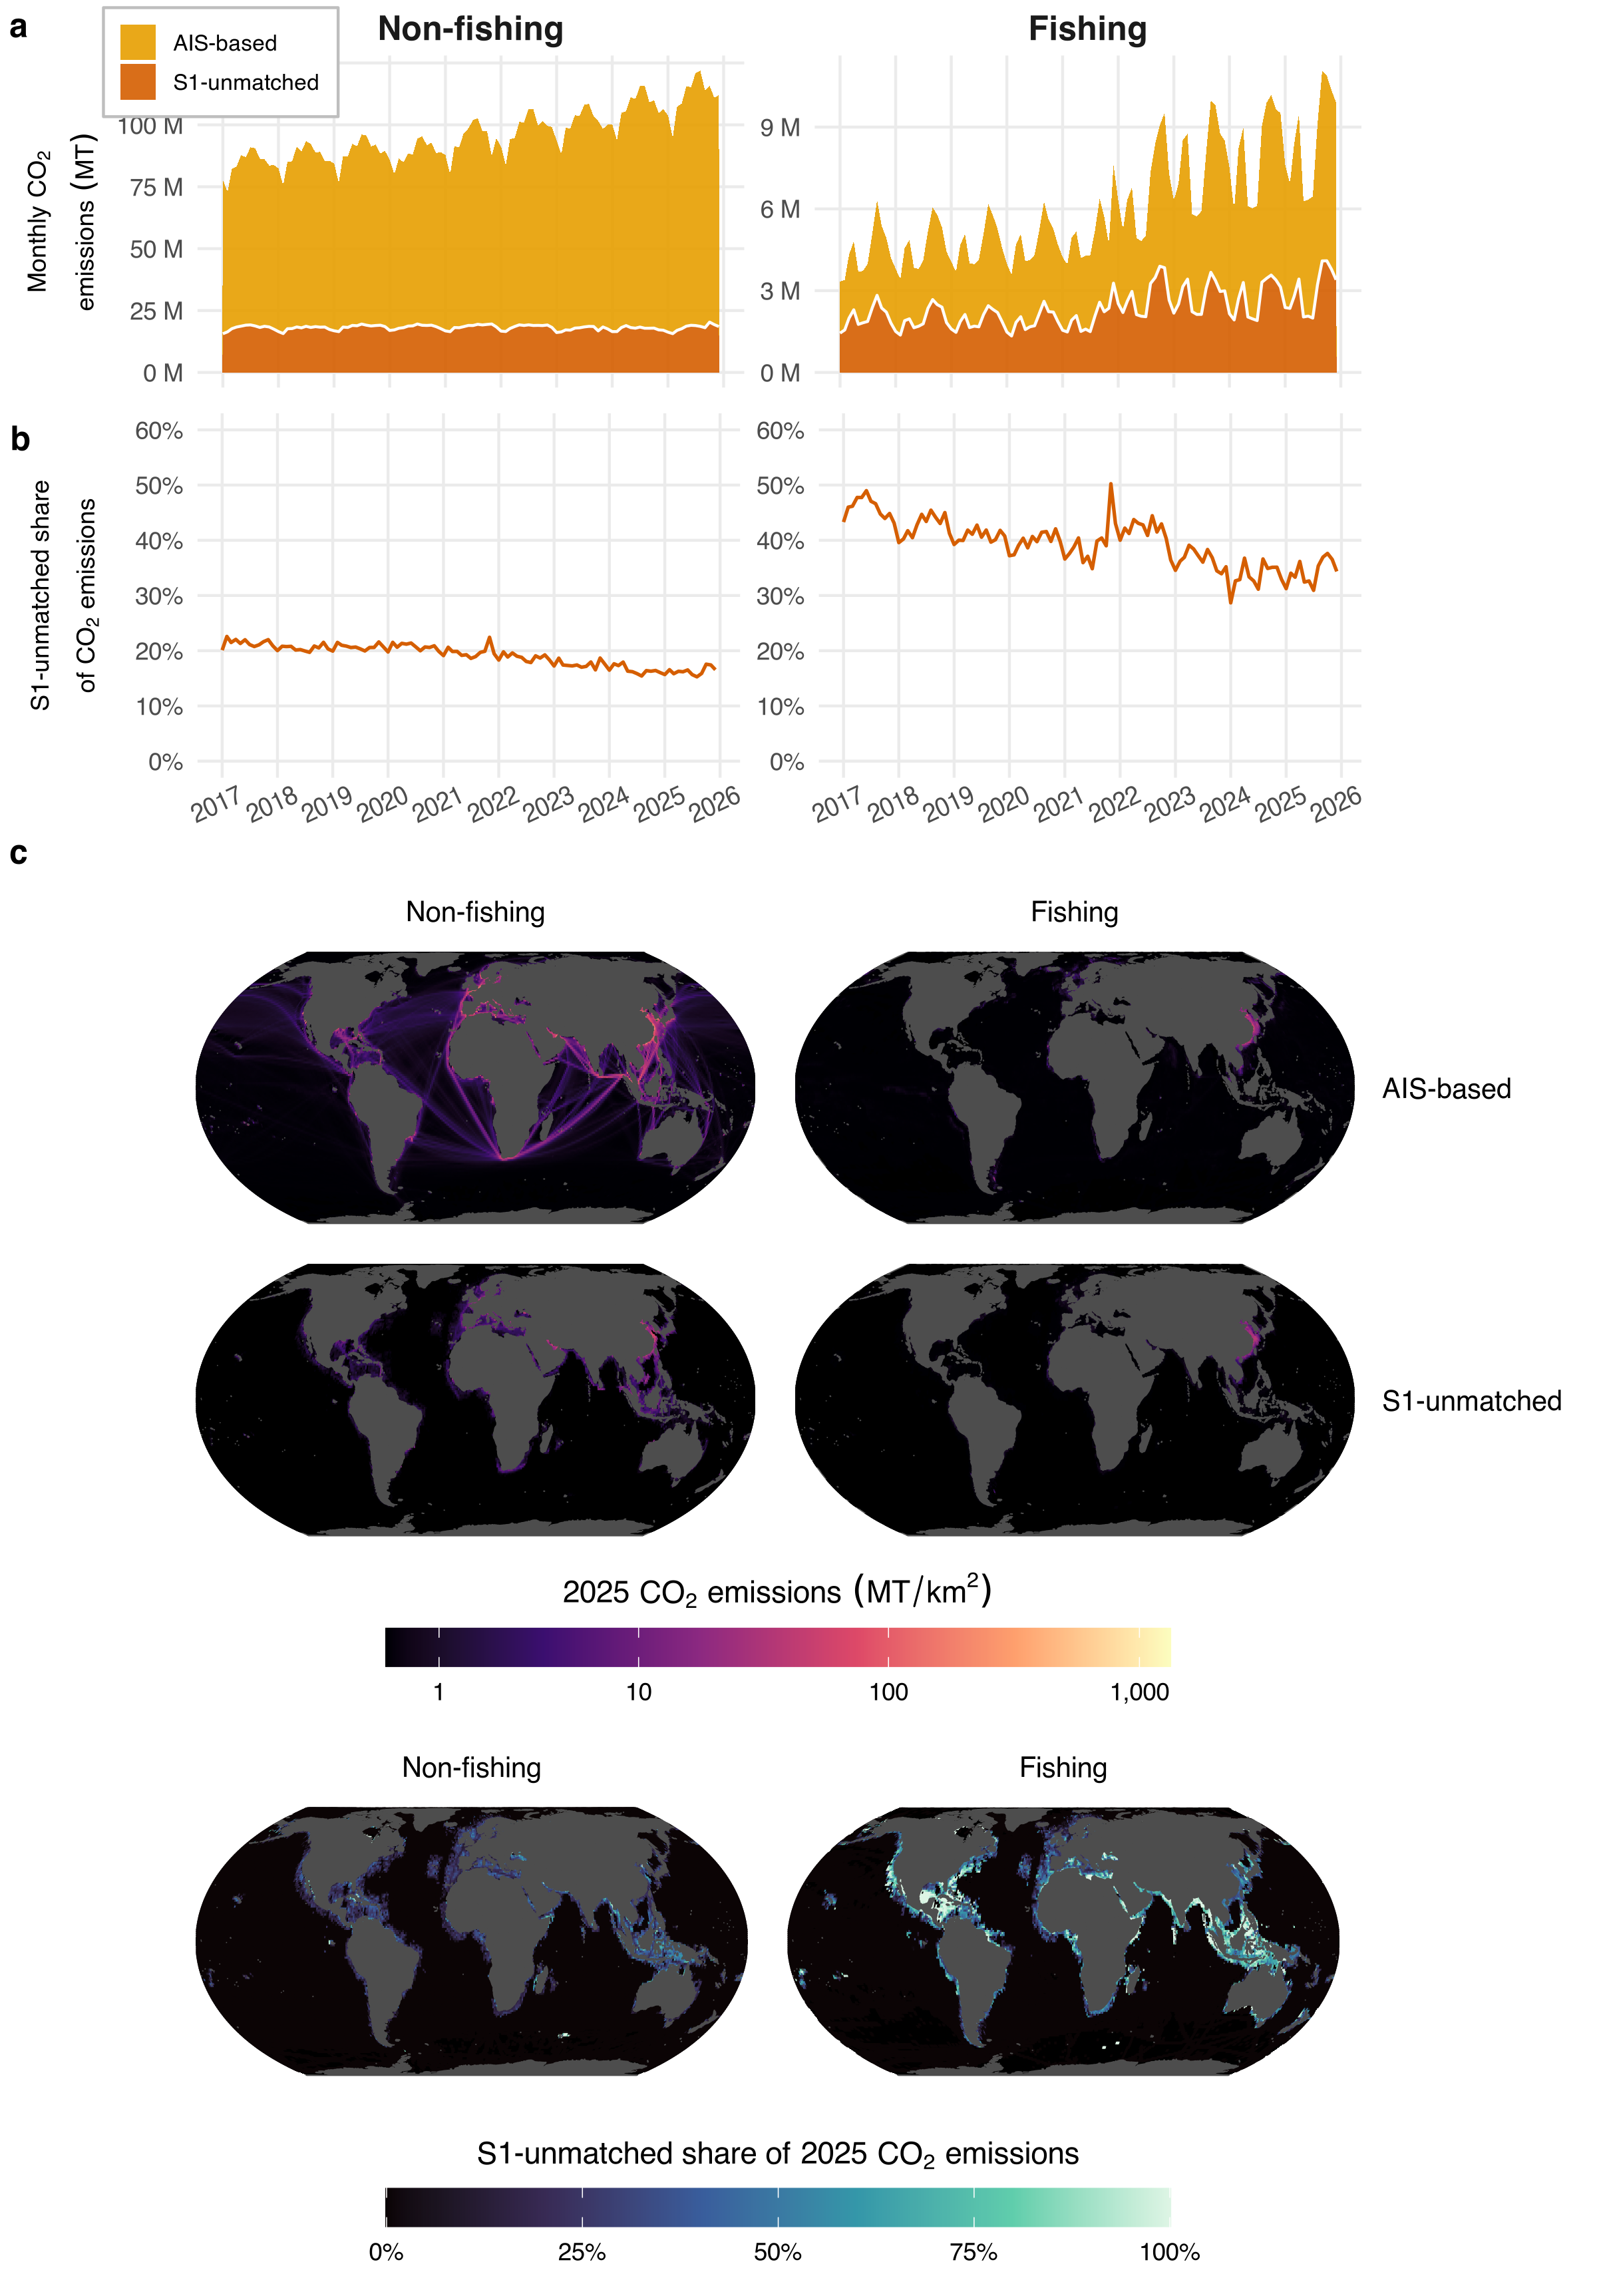
\includegraphics[width=\columnwidth]{figures/fig-spatial-temporal-richness-by-fleet-total-pseudolog-1.png}
    \caption{\DIFaddFL{The fishing and non-fishing components of Figure \ref{fig:fig-emissions-time-series-and-maps}, panel for panel. (a) Time series of monthly global CO$_2$ emissions, shown for both AIS-based and S1-unmatched emissions, and for both fishing and non-fishing vessels. (b) Time series of the monthly share of global CO$_{2}$ emissions that is S1-unmatched, for both fishing and non-fishing vessels. (c) Spatial distribution of 2025 CO$_{2}$ emissions, AIS-based (top) and S1-unmatched (middle), for both fishing and non-fishing vessels (columns), shown at a 1x1 degree spatial resolution; emissions are area-normalized for each pixel (metric tonnes per square kilometer, shown on a pseudolog-10 scale). The bottom maps show, for each pixel, the share of its 2025 CO$_{2}$ emissions from that group of vessels that is S1-unmatched; unlike the maps above them, these show a percentage and use their own color scale. Pixels with no 2025 emissions from the group are drawn in the background color, as are pixels with no emissions on the maps above.}}
    \label{fig:fig-spatial-temporal-richness-by-fleet-total-pseudolog}
\end{figure}
\DIFaddend 

\begin{figure}[H]
    \centering
    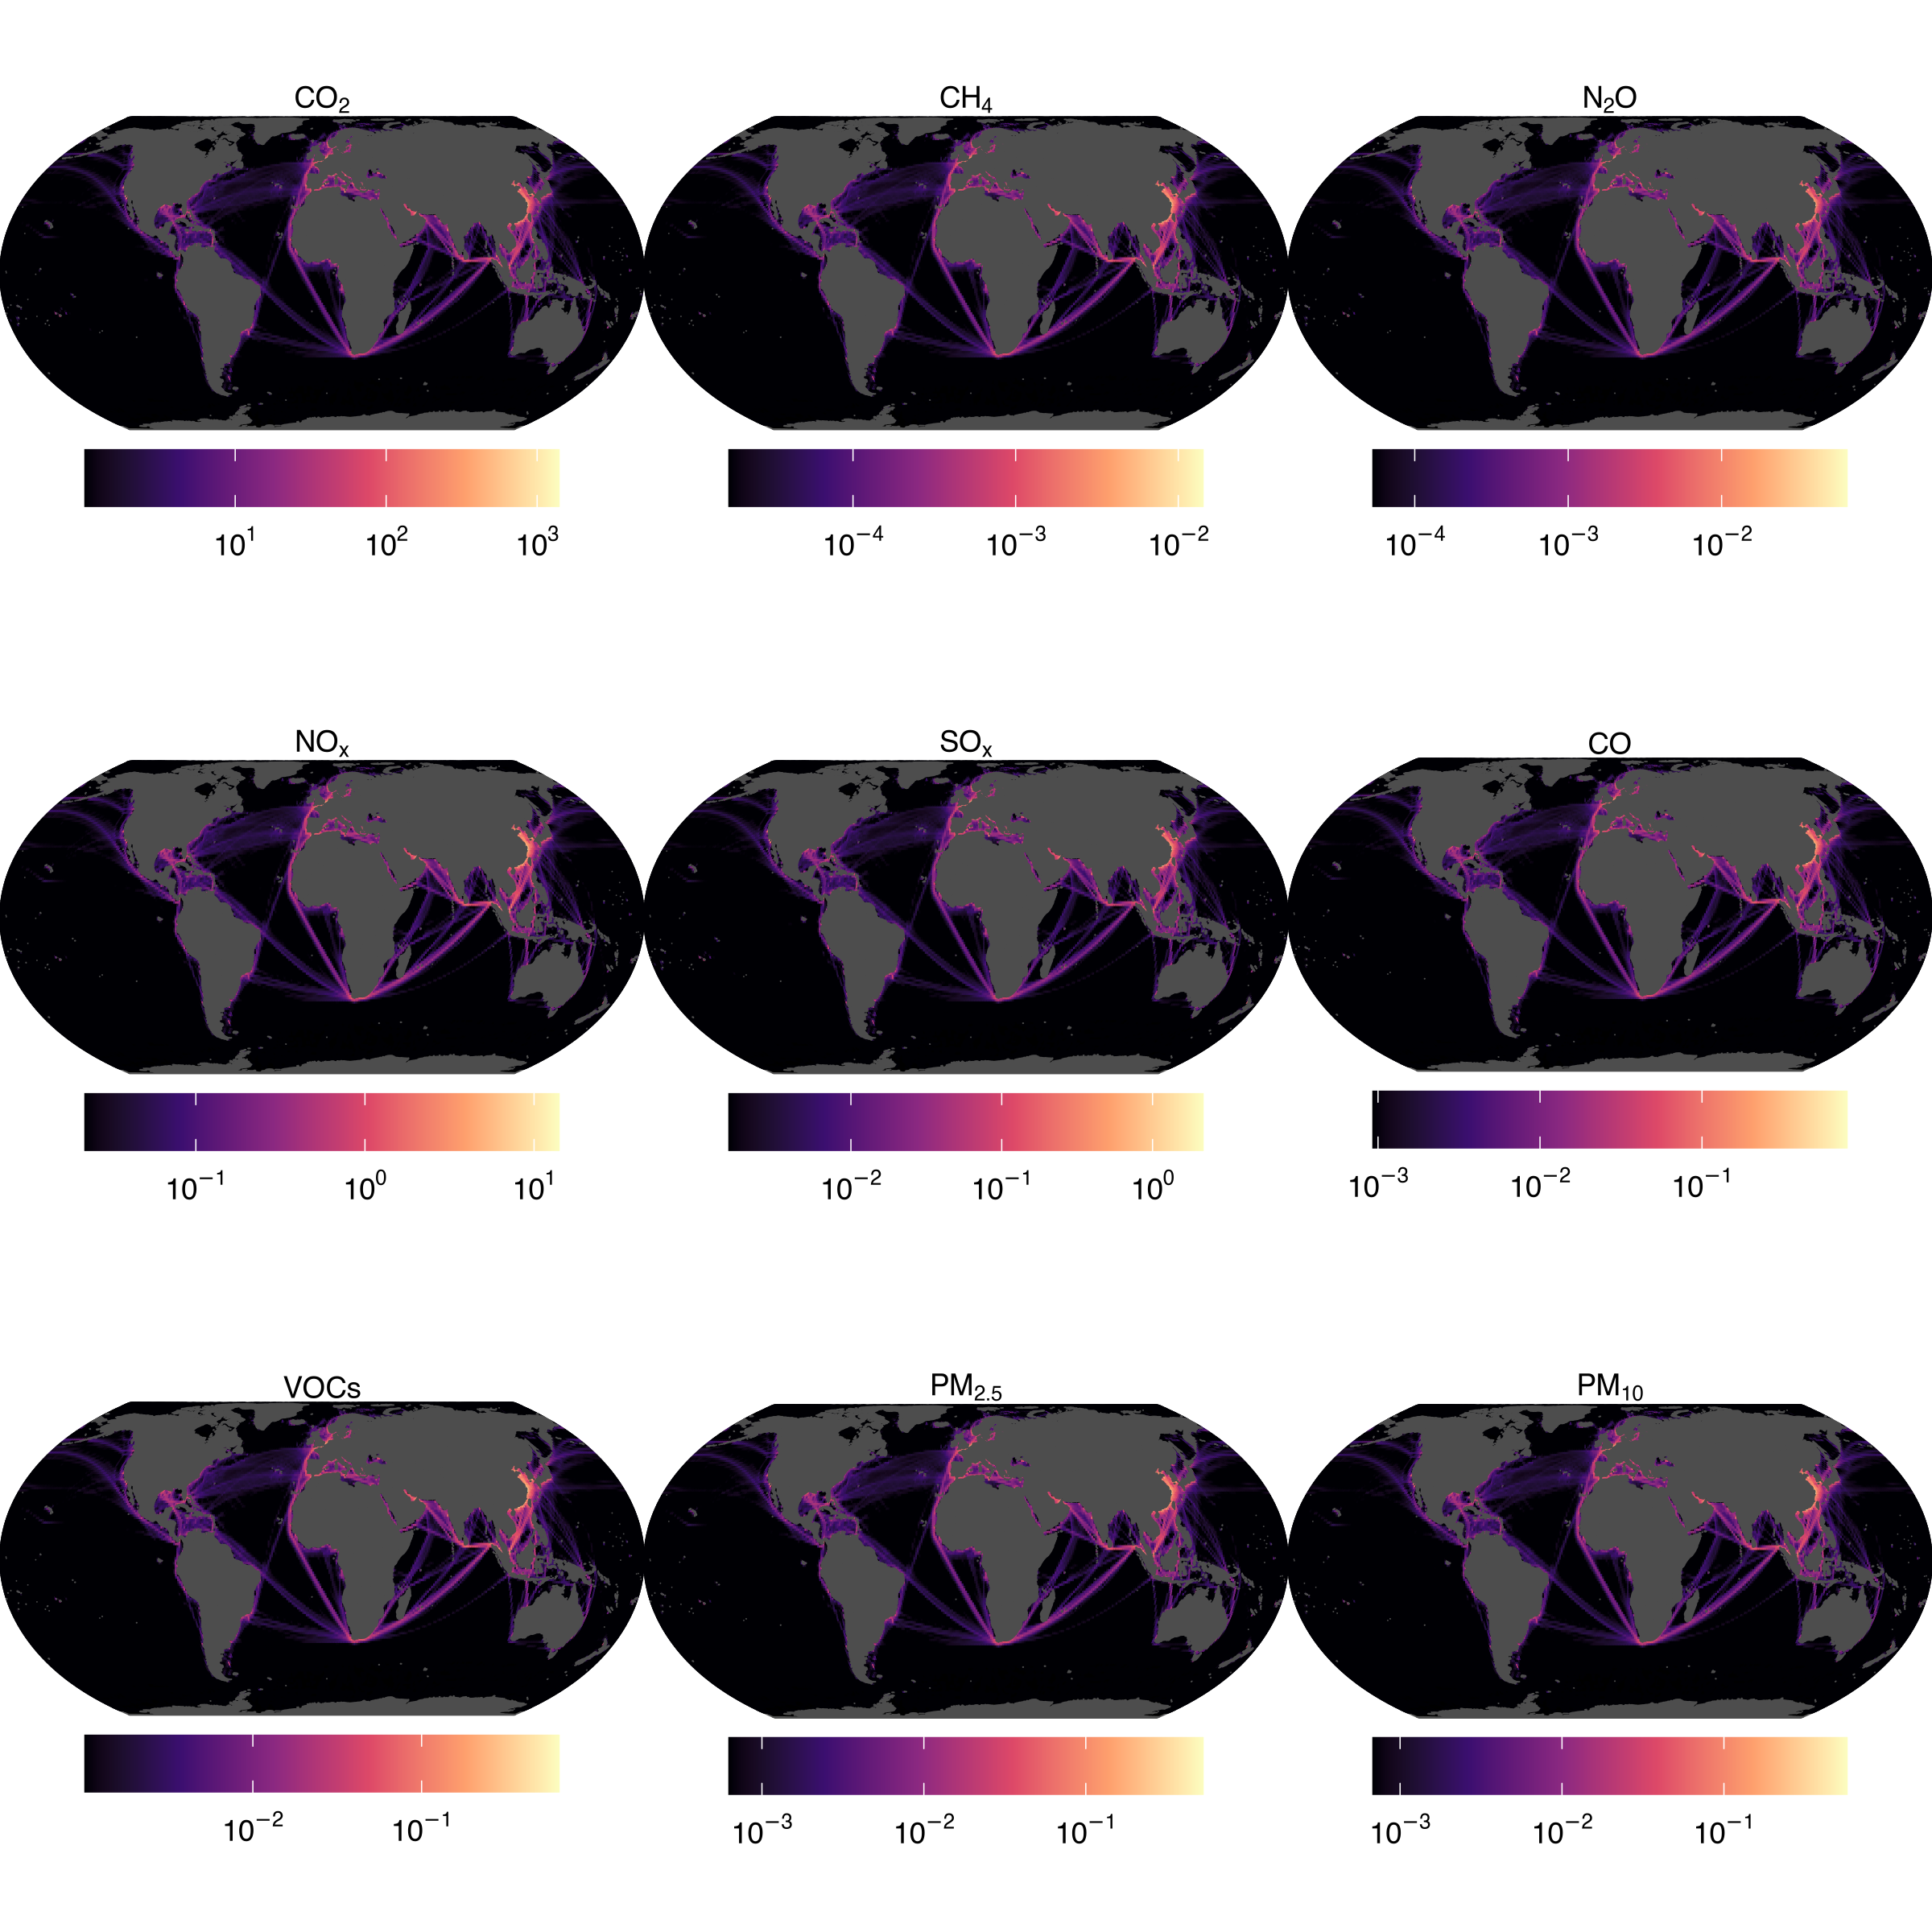
\includegraphics[width=\columnwidth]{figures/fig-pollutant-maps-qlog10-1.png}
    \DIFdelbeginFL %DIFDELCMD < \caption{%
{%DIFAUXCMD
\DIFdelFL{Spatial maps 2024 emissions for each GHG and pollutant, aggregated across AIS-broadcasting vessels and non-broadcasting vessels, and shown at a 1x1 degree spatial resolution. Emissions are area-normalized for each pixel (metric tonnes per square kilometer), and shown using a log-10 scale.}}
    %DIFAUXCMD
\DIFdelendFL \DIFaddbeginFL \caption{\DIFaddFL{Spatial maps of 2025 emissions for each GHG and pollutant, aggregated across AIS-based and S1-unmatched emissions, and shown at a 1x1 degree spatial resolution. Emissions are area-normalized for each pixel (metric tonnes per square kilometer) and shown using a log-10 scale. Each panel is scaled independently, spanning the 75th percentile to the maximum of that pollutant, with lower values drawn in the darkest color; colors are therefore not comparable between panels.}}
    \DIFaddendFL \label{fig:fig-pollutant-maps}
\end{figure}

\begin{figure}[H]
    \centering
    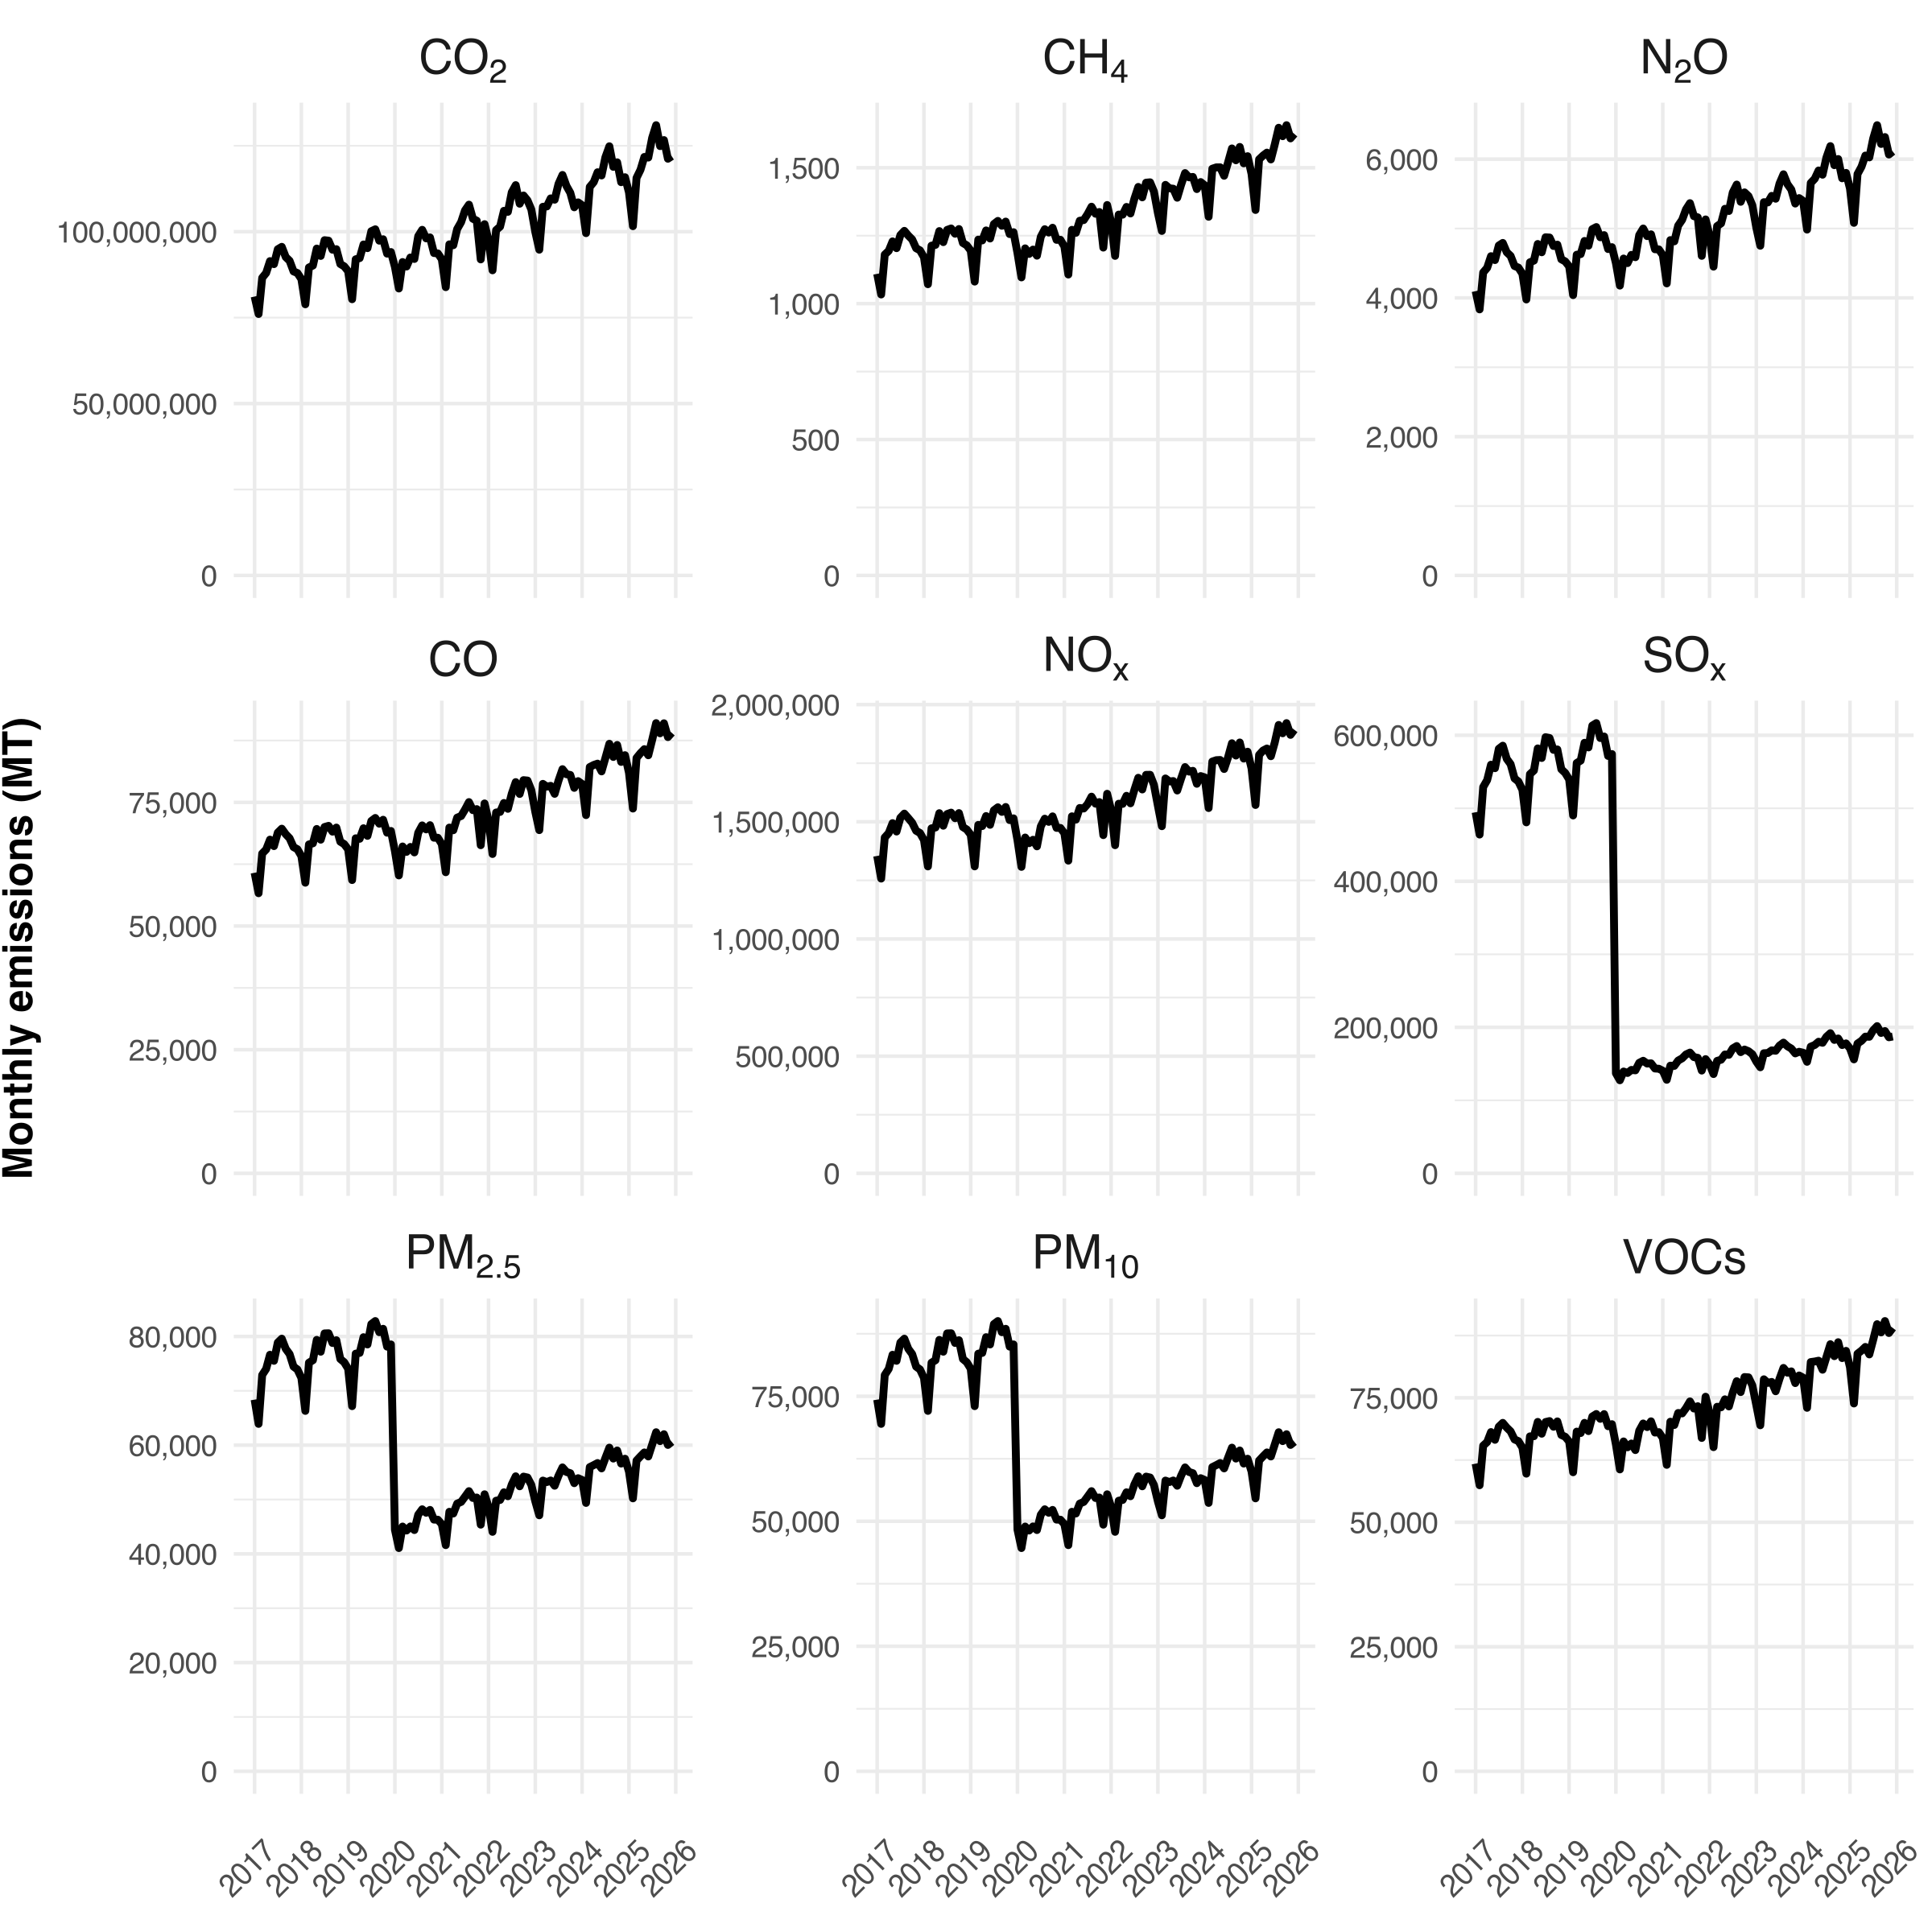
\includegraphics[width=\columnwidth]{figures/fig-pollutant-time-series-1.png}
    \DIFdelbeginFL %DIFDELCMD < \caption{%
{%DIFAUXCMD
\DIFdelFL{Time series of monthly global emissions for each GHG and pollutant, aggregated across AIS-broadcasting vessels and non-broadcasting vessels for which we only have Sentinel-1 data.}}
    %DIFAUXCMD
\DIFdelendFL \DIFaddbeginFL \caption{\DIFaddFL{Time series of monthly global emissions for each GHG and pollutant, aggregated across AIS-based and S1-unmatched emissions.}}
    \DIFaddendFL \label{fig:fig-pollutant-time-series}
\end{figure}

\begin{figure}[H]
    \centering
    \DIFaddbeginFL 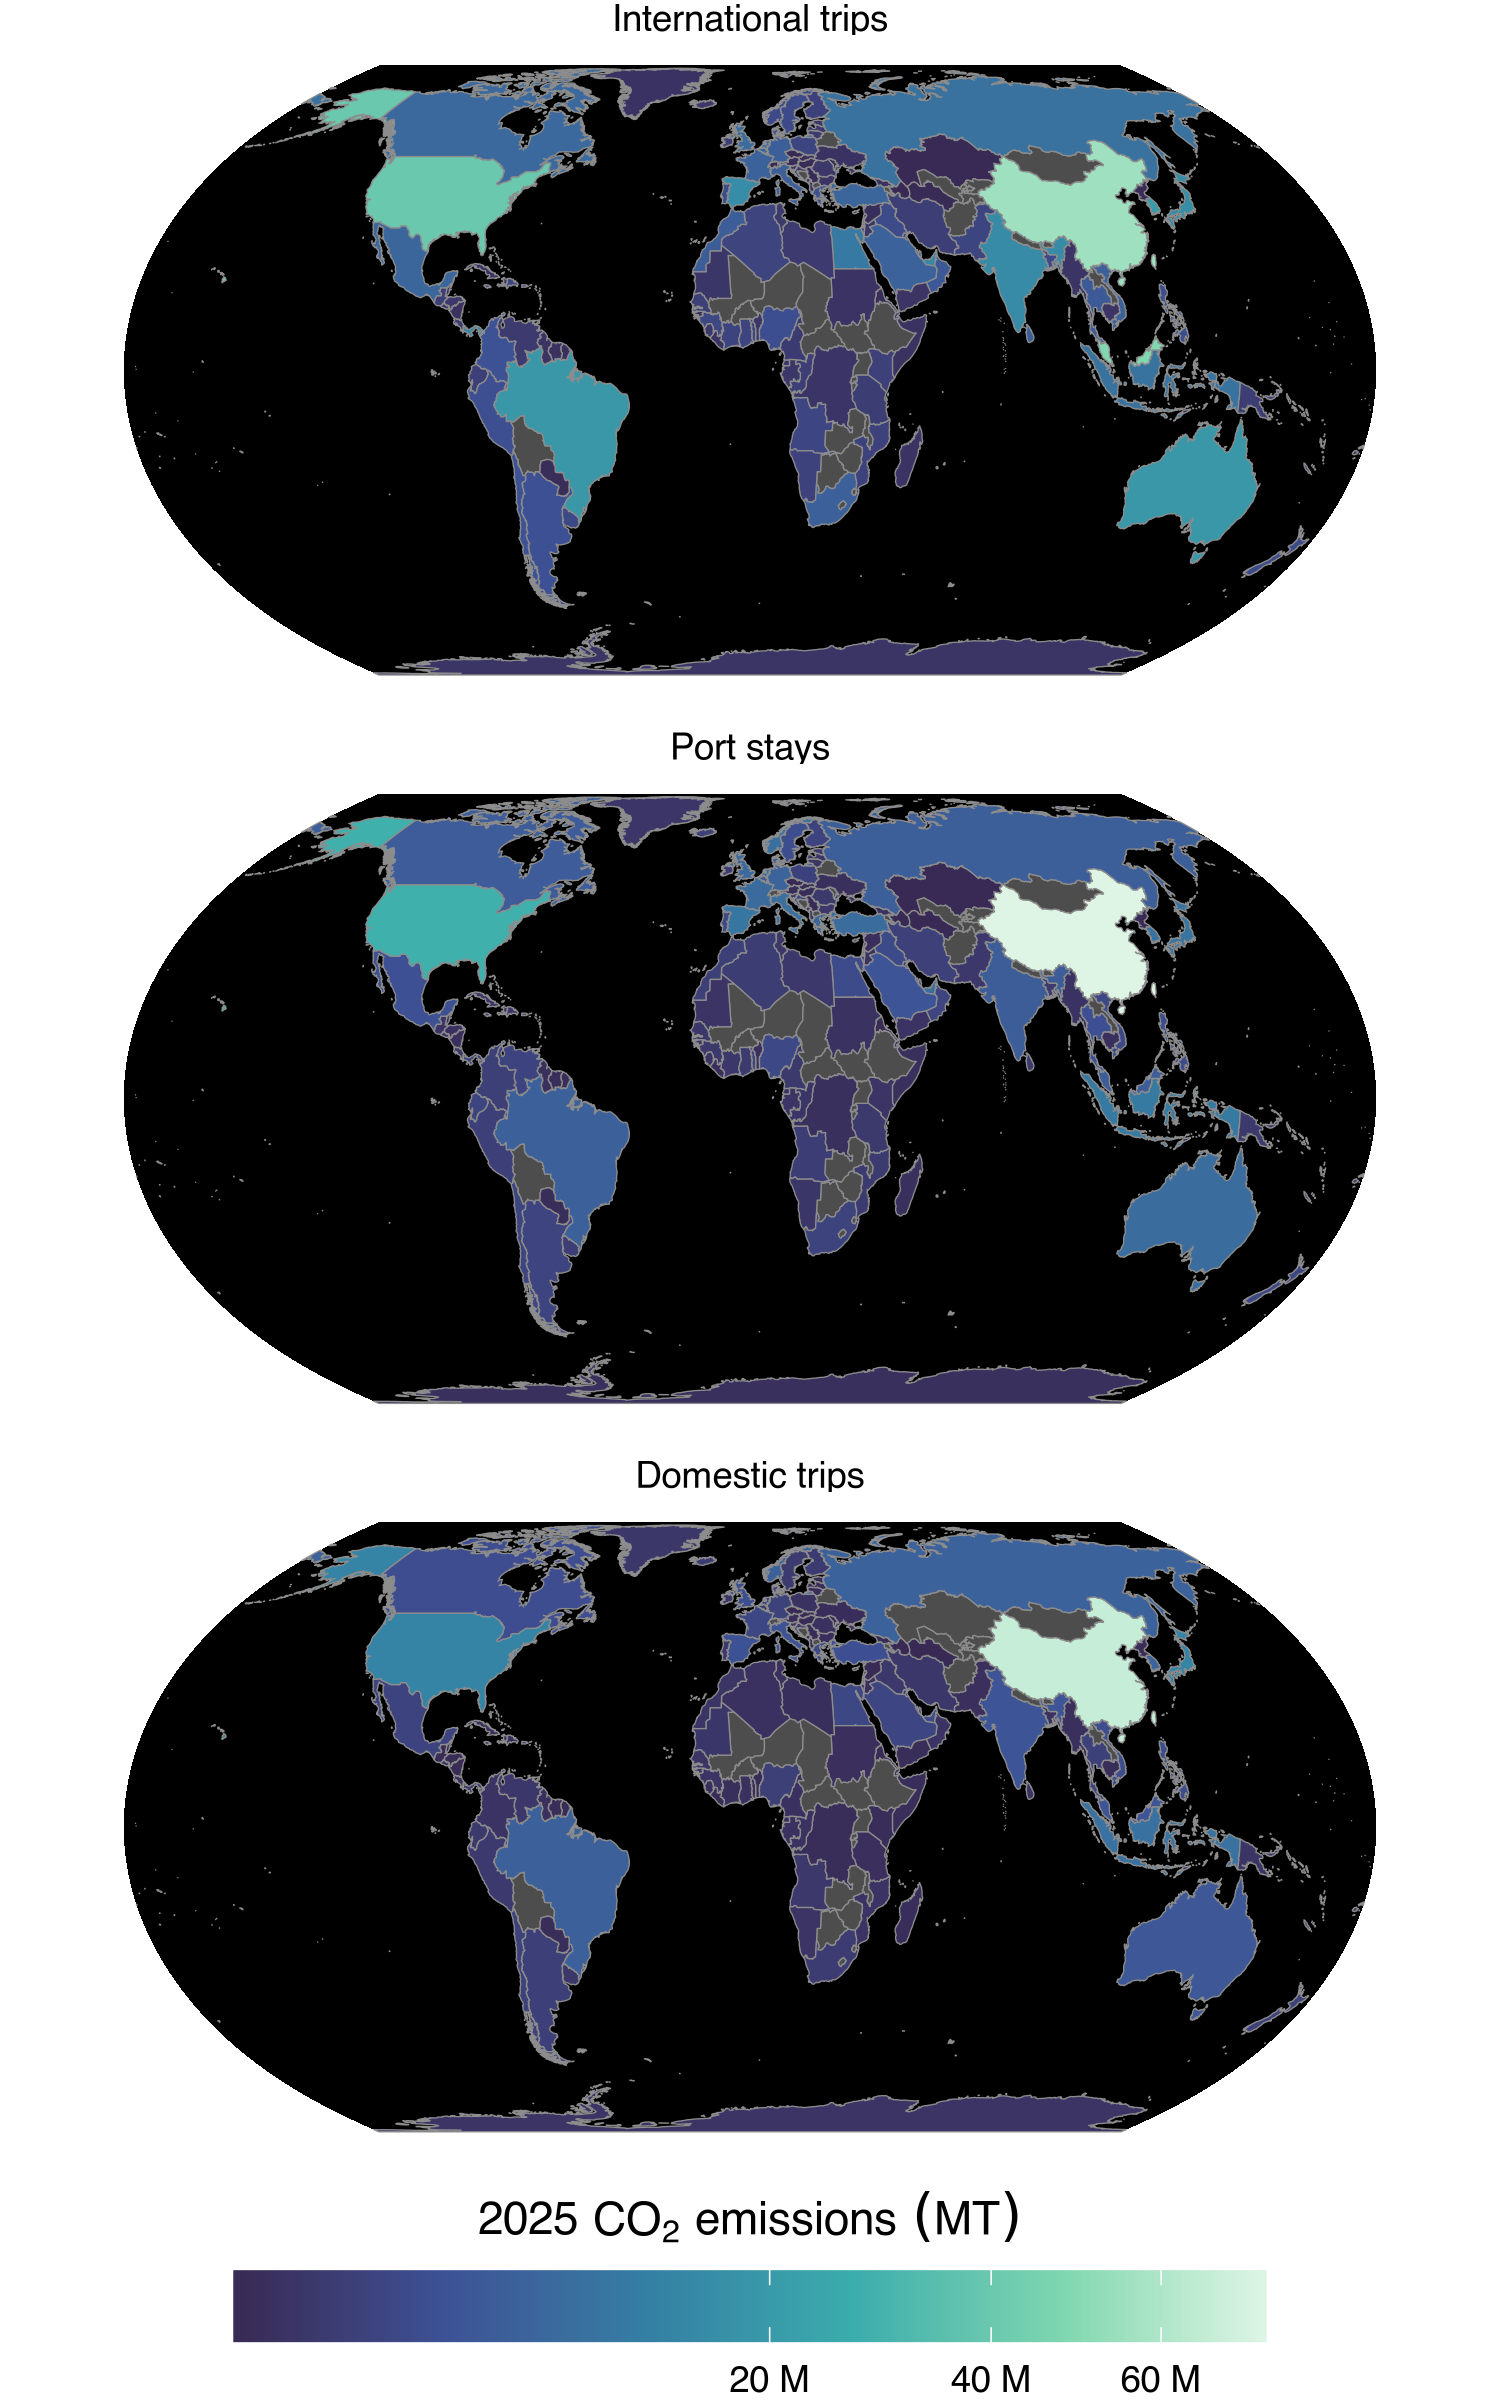
\includegraphics[width=0.85\columnwidth]{figures/fig-emissions-by-country-and-activity-type-1.png}
    \caption{\DIFaddFL{CO$_{2}$ emissions by country for AIS-broadcasting vessels during different activity types (international trips, port stays, and domestic trips), aggregated for activities ending in 2025. Emissions for each international trip are partitioned equally to its departure and arrival country. The color scale is square-root transformed, so that lower-emitting countries remain distinguishable alongside the largest emitters. Countries with no values are shown in gray.}}
    \label{fig:fig-emissions-by-country-and-activity-type}
\end{figure}

\begin{figure}[H]
    \centering
    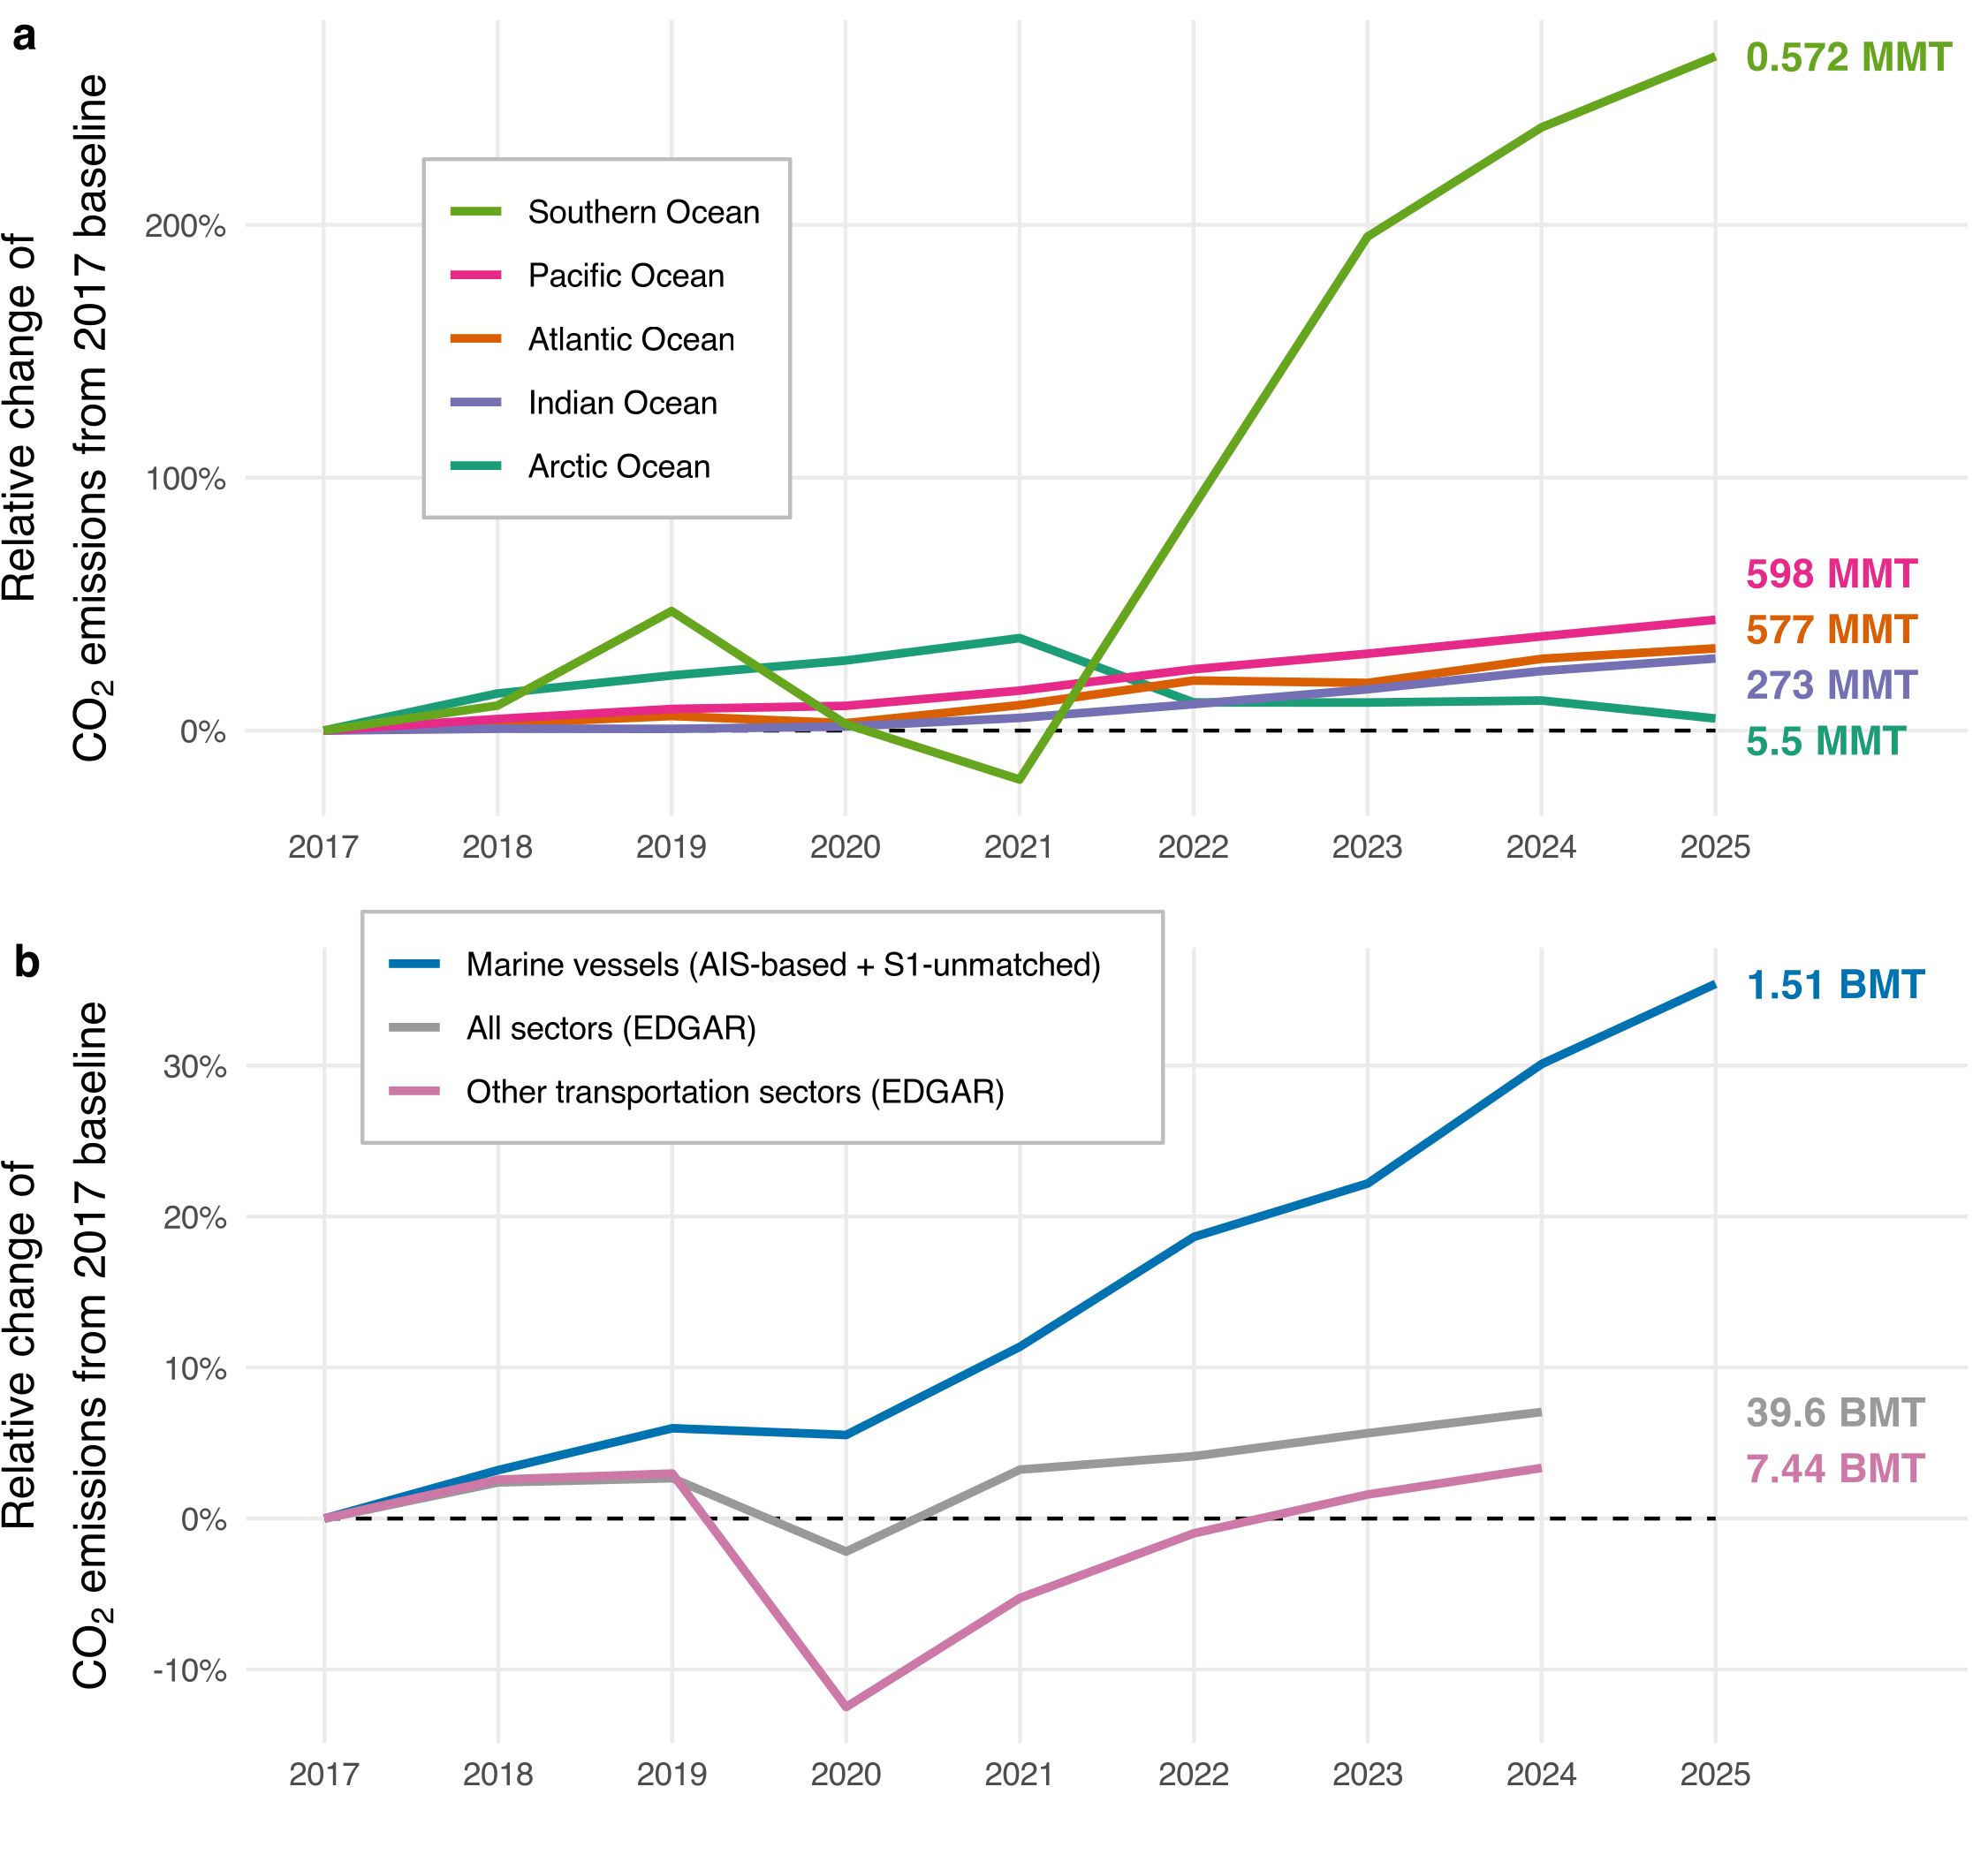
\includegraphics[width=\columnwidth]{figures/fig-emissions-marine-ocean-other-1.png}
    \caption{\DIFaddFL{Trend in CO$_{2}$ emissions by ocean (normalized to 2017 baseline), using our fused (AIS-based + S1-unmatched) estimates. On the right-hand side of the figure, absolute values for the last year of available data (2025) are shown as text and color-coded for each line.}}
    \label{fig:fig-emissions-marine-ocean-other}
\end{figure}

\begin{figure}[H]
    \centering
    \DIFaddendFL 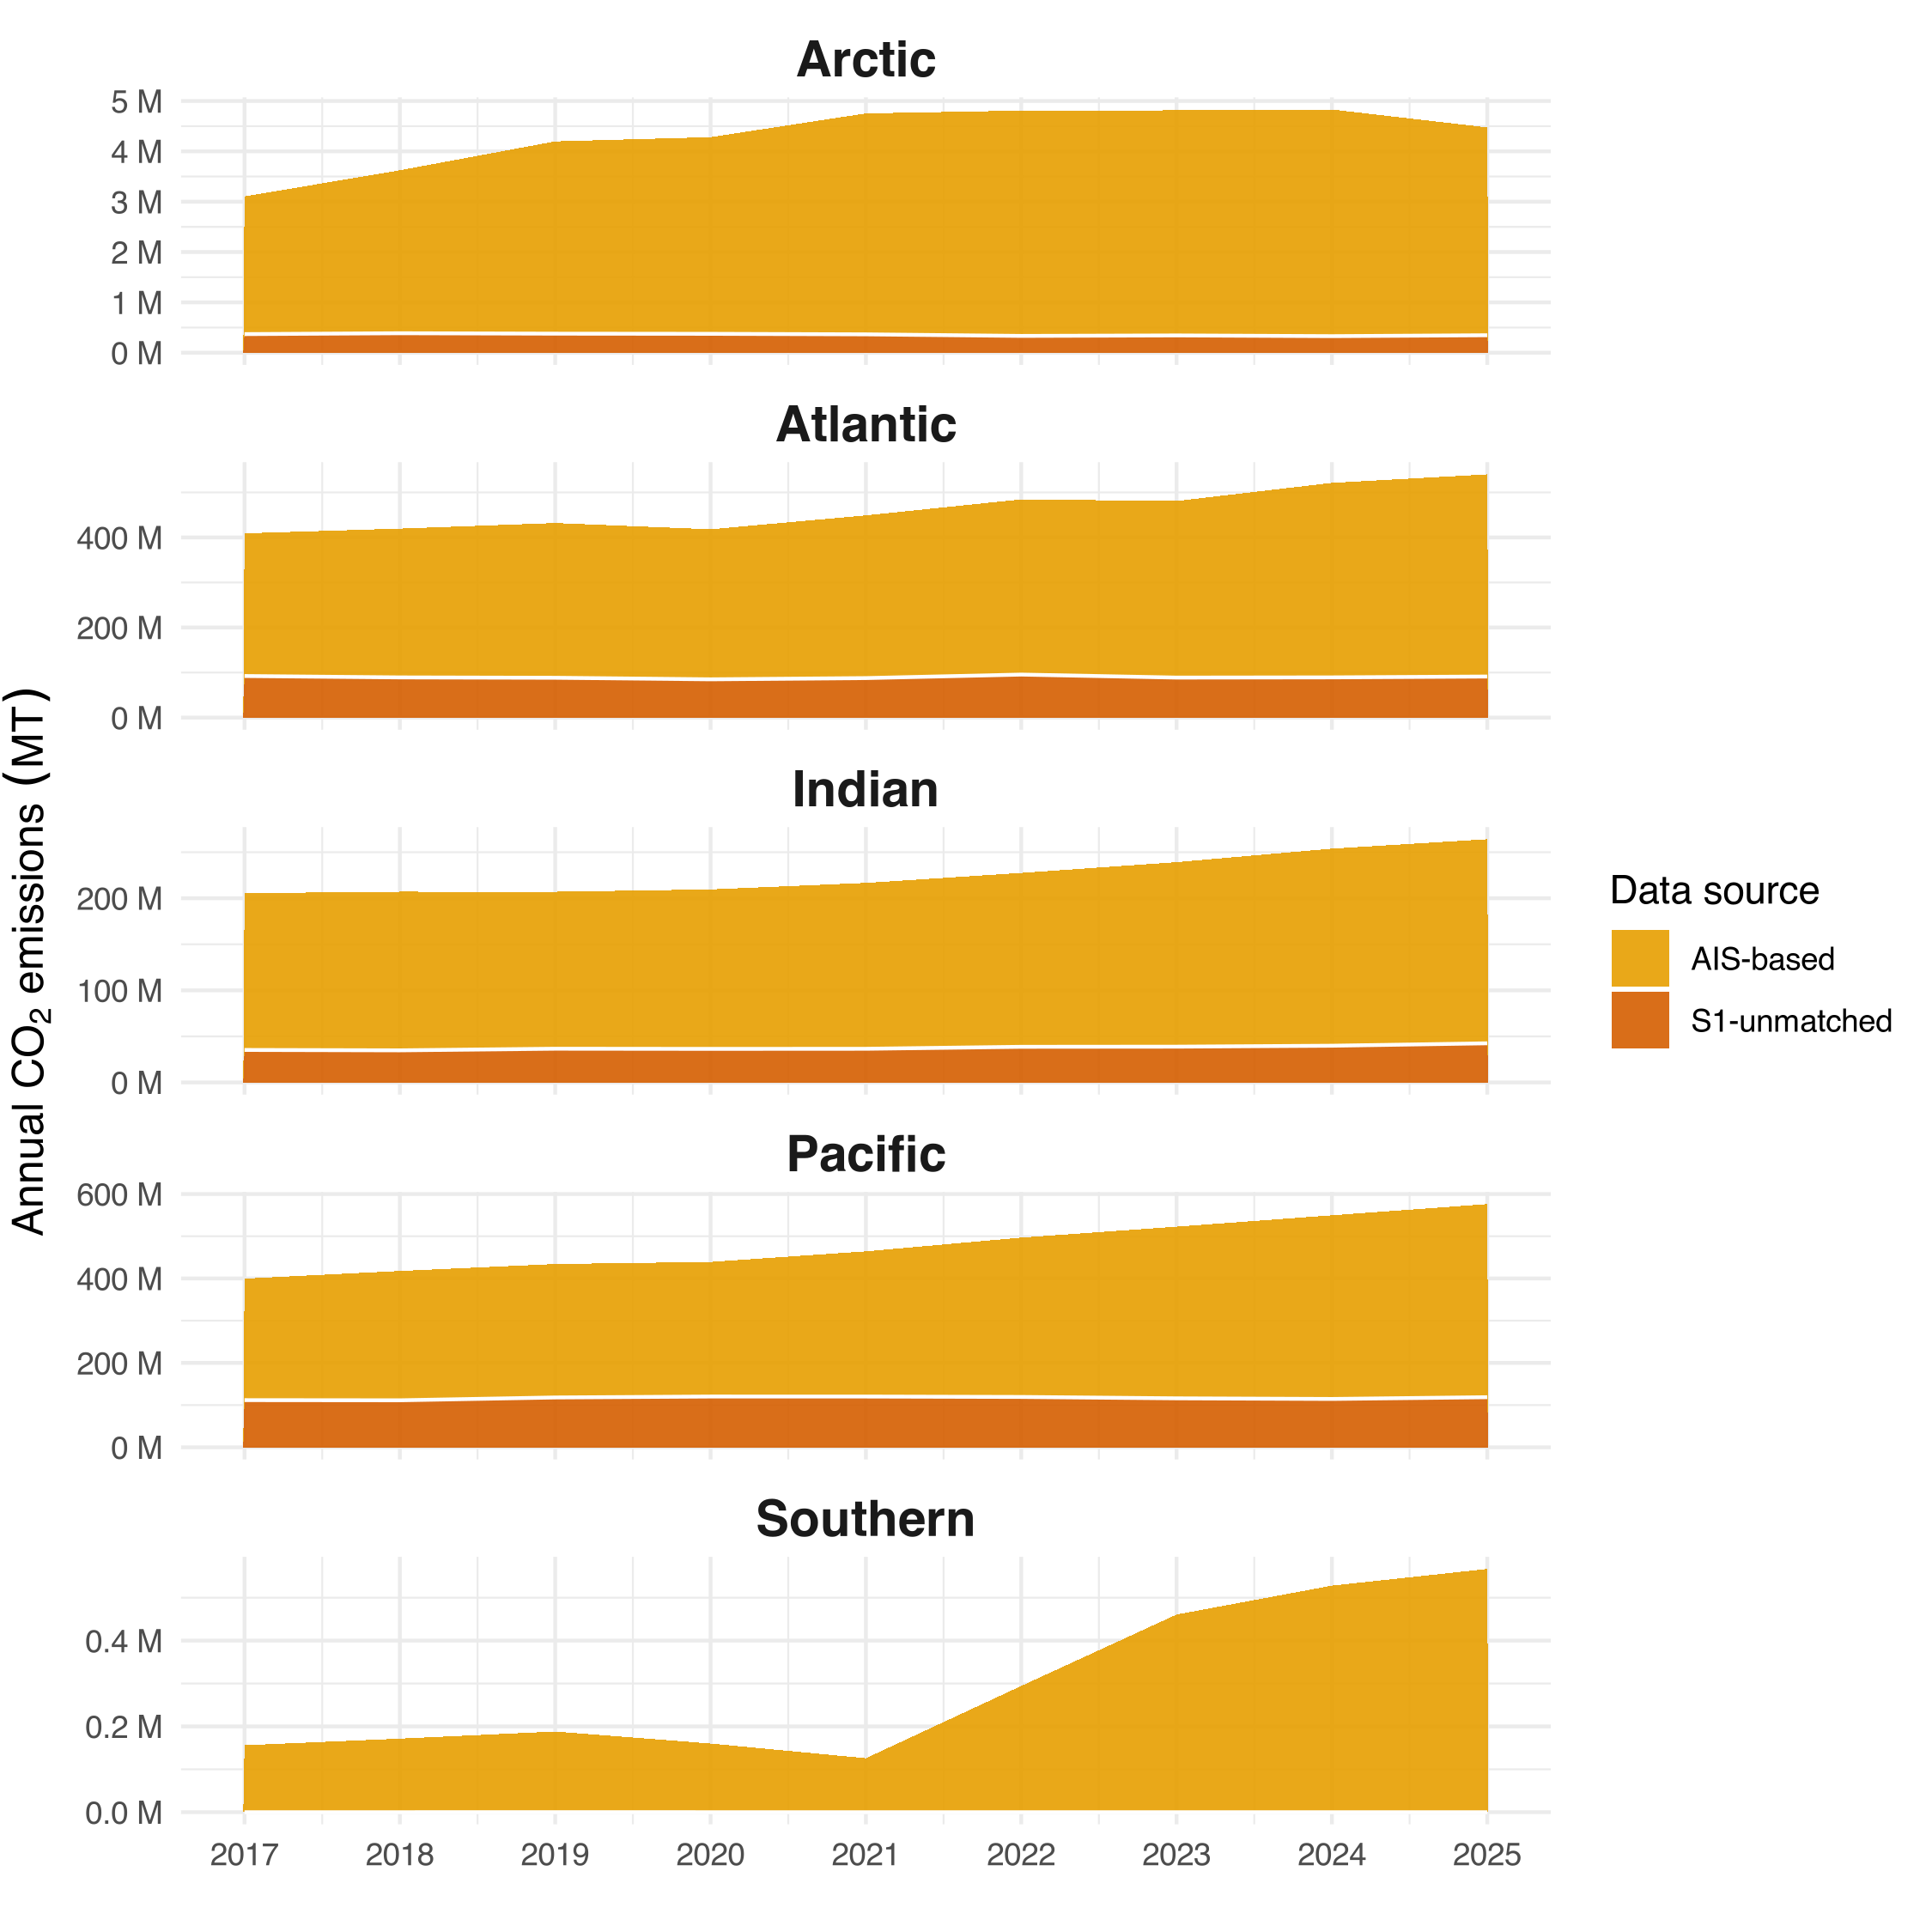
\includegraphics[width=\columnwidth]{figures/fig-annual-emissions-by-ocean-and-data-source-1.png}
    \DIFdelbeginFL %DIFDELCMD < \caption{%
{%DIFAUXCMD
\DIFdelFL{Annual total CO2 emissions by ocean, disaggregated by data source (AIS-broadcasting vessels, and non-broadcasting vessels detected by S1).}}
    %DIFAUXCMD
\DIFdelendFL \DIFaddbeginFL \caption{\DIFaddFL{Annual total CO$_{2}$ emissions by ocean, disaggregated by data source (AIS-based and S1-unmatched).}}
    \DIFaddendFL \label{fig:fig-annual-emissions-by-ocean-and-data-source}
\end{figure}

\DIFdelbegin \subsection{\DIFdel{Supplementary Tables}}
%DIFAUXCMD
\addtocounter{subsection}{-1}%DIFAUXCMD
\DIFdelend \DIFaddbegin \begin{figure}[!p]
    \centering
    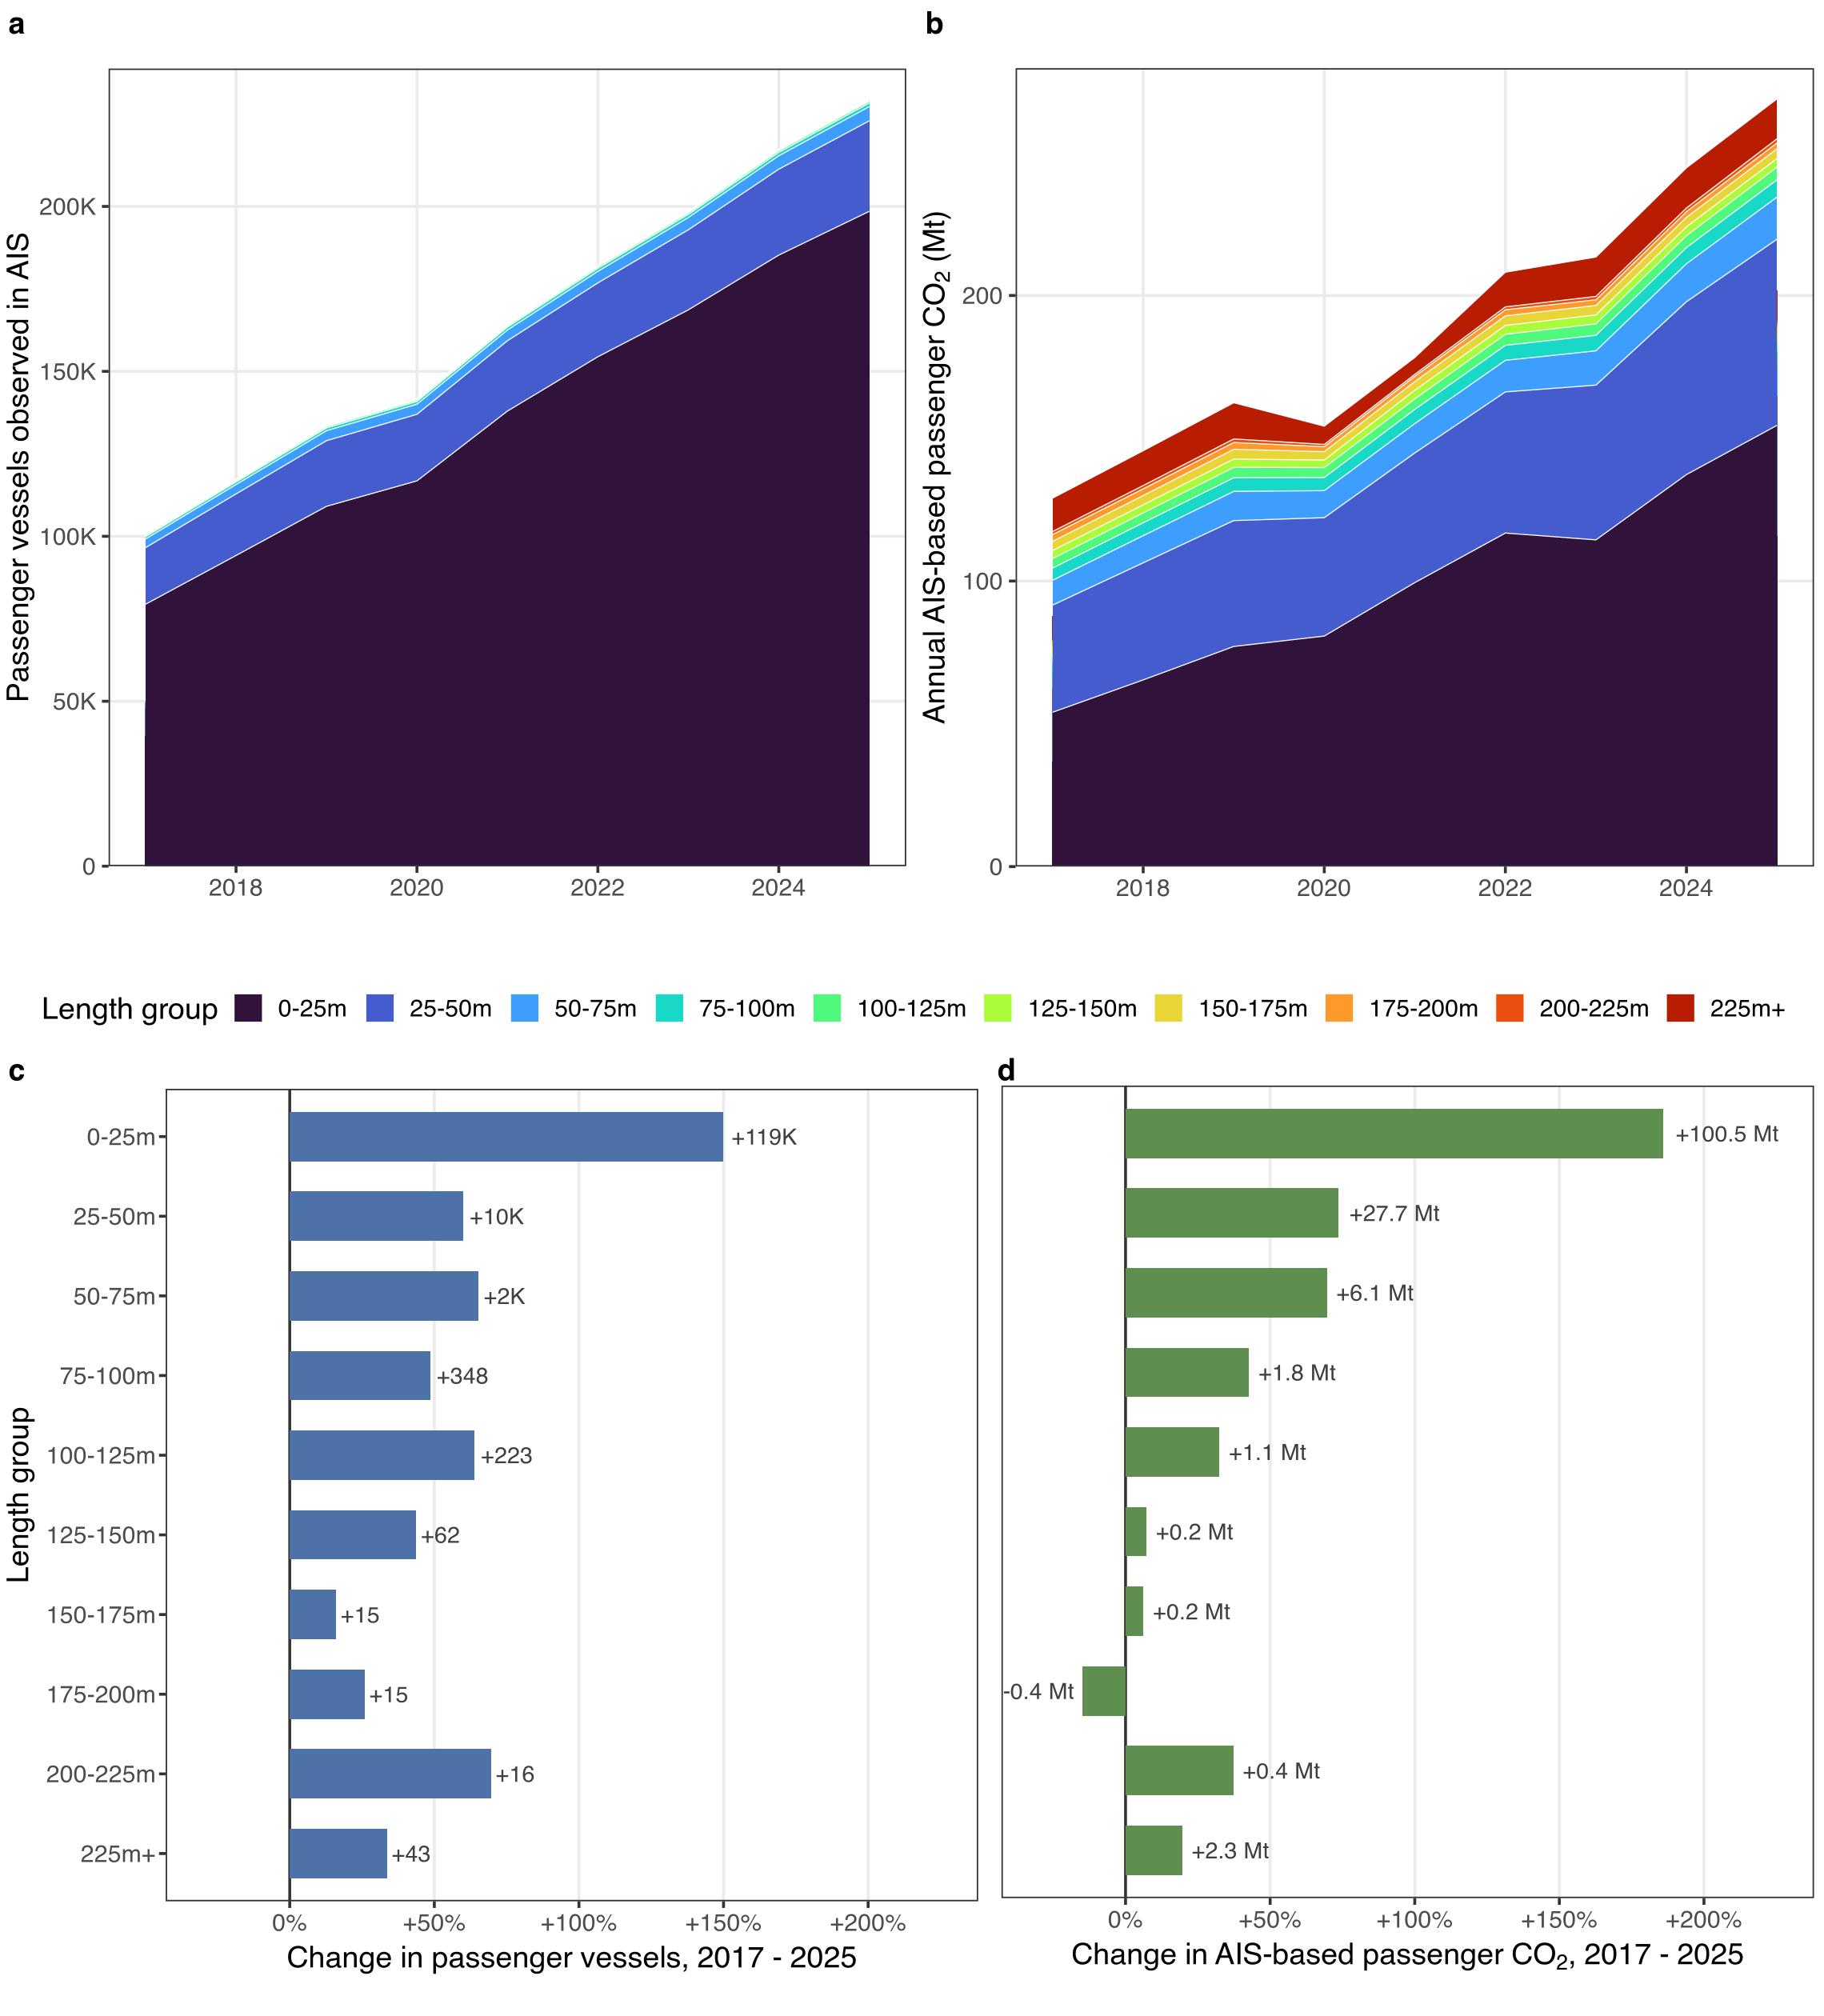
\includegraphics[width=\columnwidth,height=0.92\textheight,keepaspectratio]{figures/figS-passenger-size-panels-1.png}
    \caption{\DIFaddFL{Passenger vessels by length bin, 2017 against 2025, showing growth concentrated in the smallest sizes.}}
    \label{fig:figS-passenger-size-panels}
\end{figure}
\DIFaddend 

\DIFaddbegin \begin{figure}[H]
    \centering
    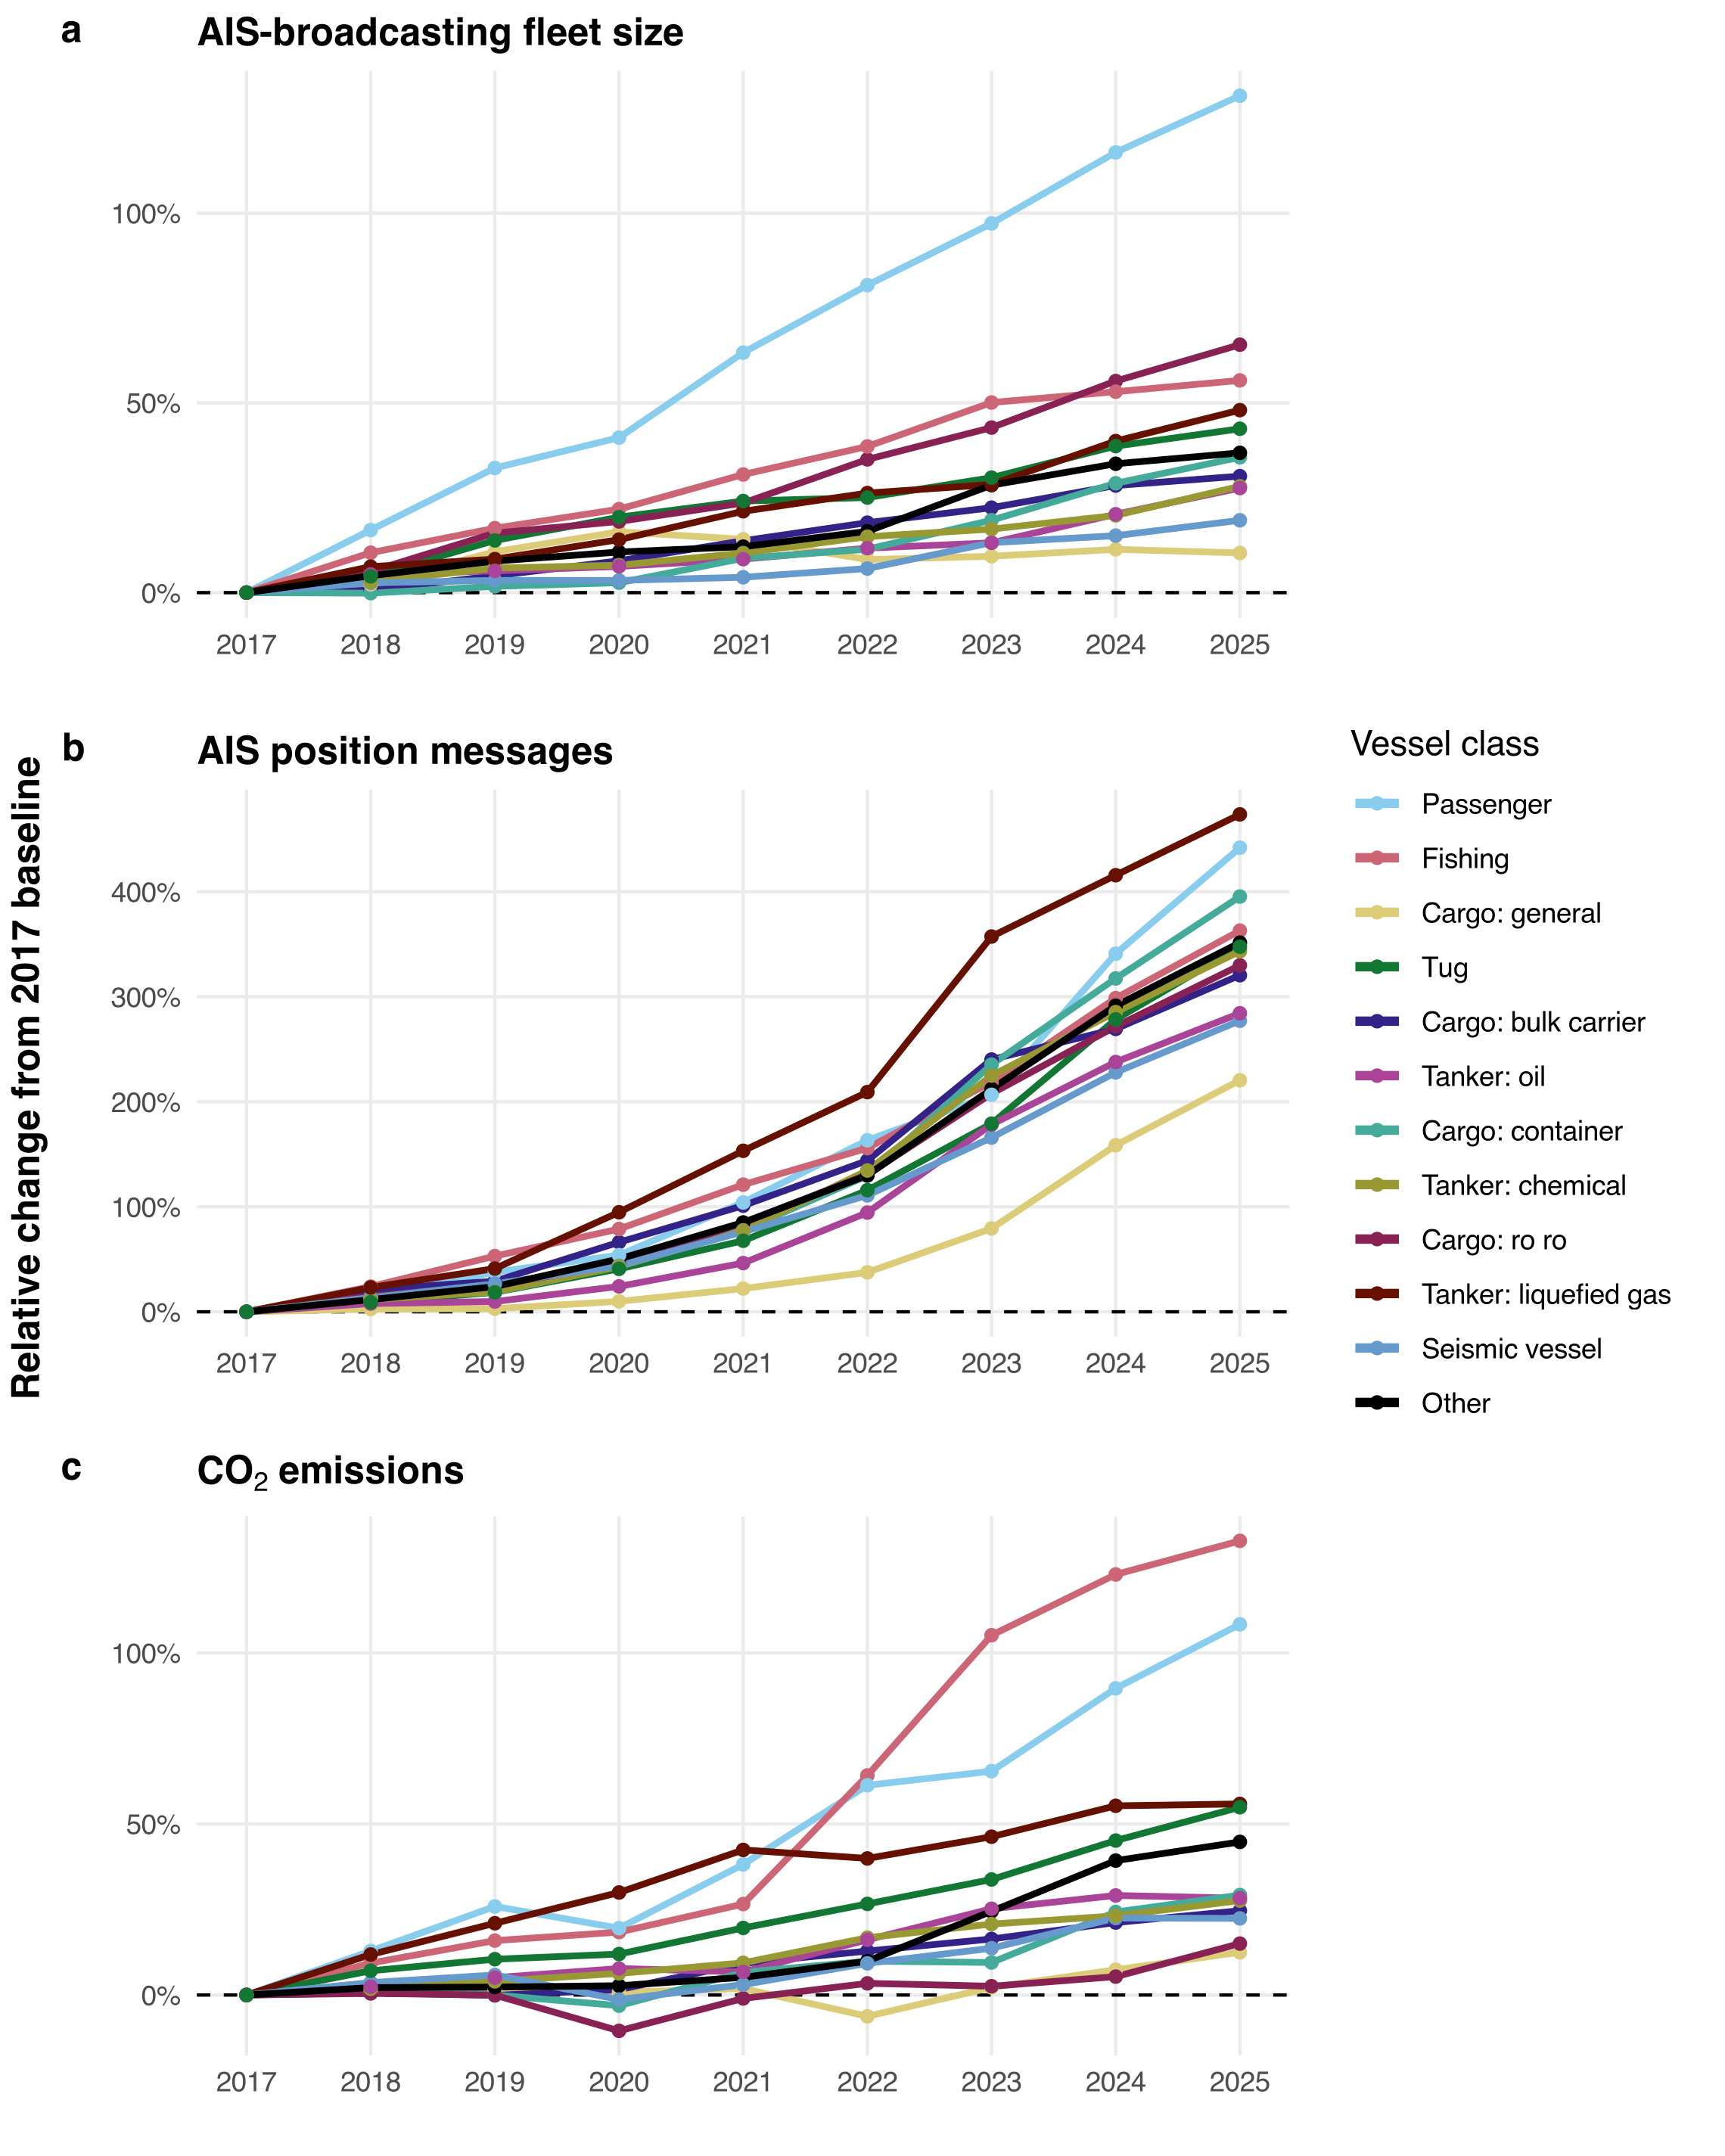
\includegraphics[width=\columnwidth]{figures/figS-fleet-growth-by-year-1.png}
    \caption{\DIFaddFL{Relative change since 2017, by vessel class, in (a) the number of AIS-broadcasting vessels, (b) AIS position messages received, and (c) CO$_{2}$ emissions, for AIS-broadcasting vessels. Every panel is expressed as a change from that class's own 2017 value, so classes of very different absolute size can be read on a single scale. Growth in panels a and b reflects both real expansion of the fleet and its activity, and the increasing uptake and reception of AIS over the period. Passenger vessels grow fastest in fleet size and fishing vessels fastest in emissions, the two classes that other inventories are least likely to cover.}}
    \label{fig:figS-fleet-growth-by-year}
\end{figure}

\begin{figure}[H]
    \centering
    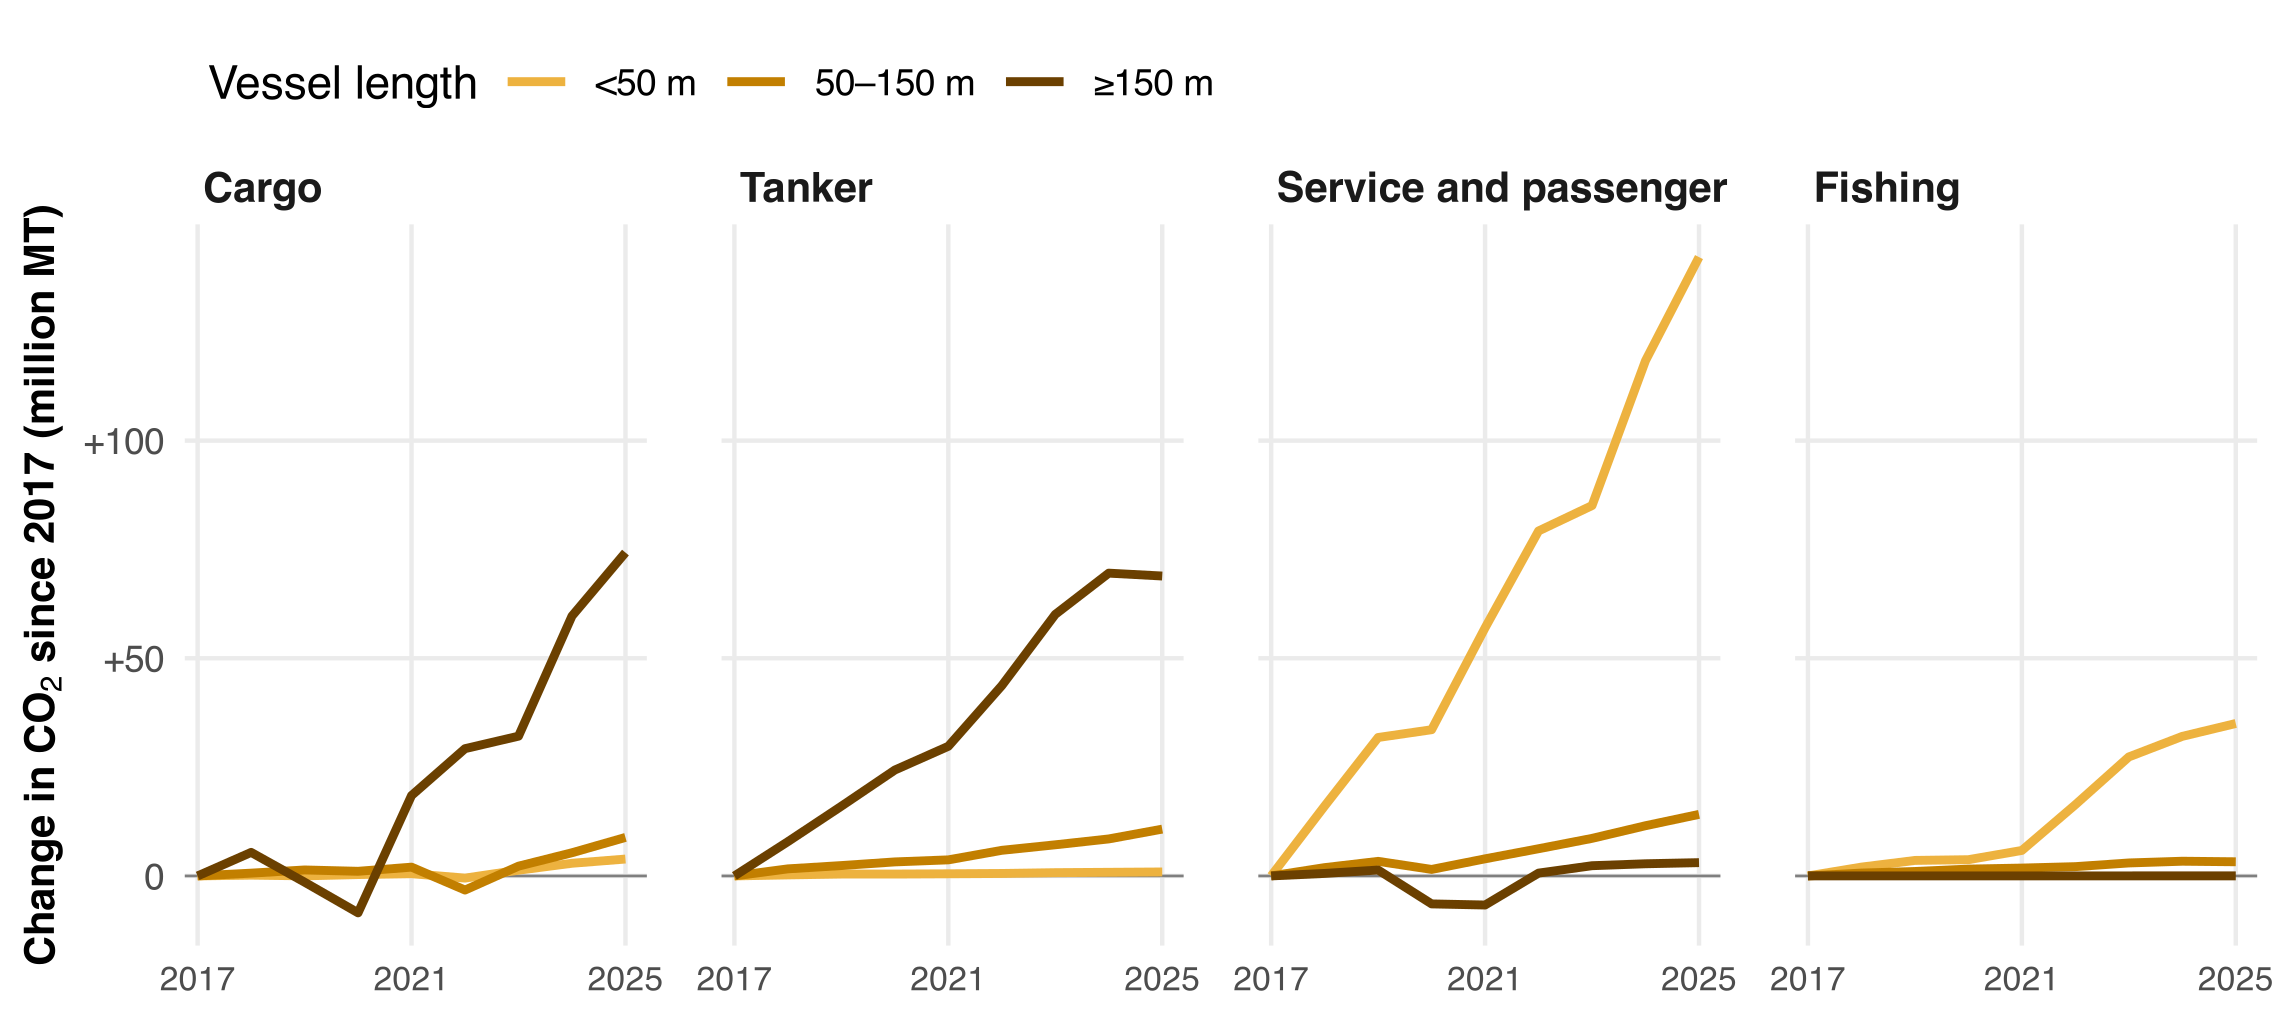
\includegraphics[width=\columnwidth]{figures/figS-growth-timeline-by-family-length-1.png}
    \caption{\DIFaddFL{Change in AIS-based CO$_{2}$ emissions since 2017, by vessel class family and length band. Each line is a segment's annual emissions minus its 2017 emissions. Families are as in Fig. \ref{fig:fig-ais-data-richness} and length bands as in Supplementary Tables \ref{tab:growth_share_by_family_length} and \ref{tab:growth_decomposition_by_family_length}, so each line ends at that segment's emissions change in Supplementary Table \ref{tab:growth_decomposition_by_family_length}.}}
    \label{fig:figS-growth-timeline-by-family-length}
\end{figure}

\begin{figure}[H]
    \centering
    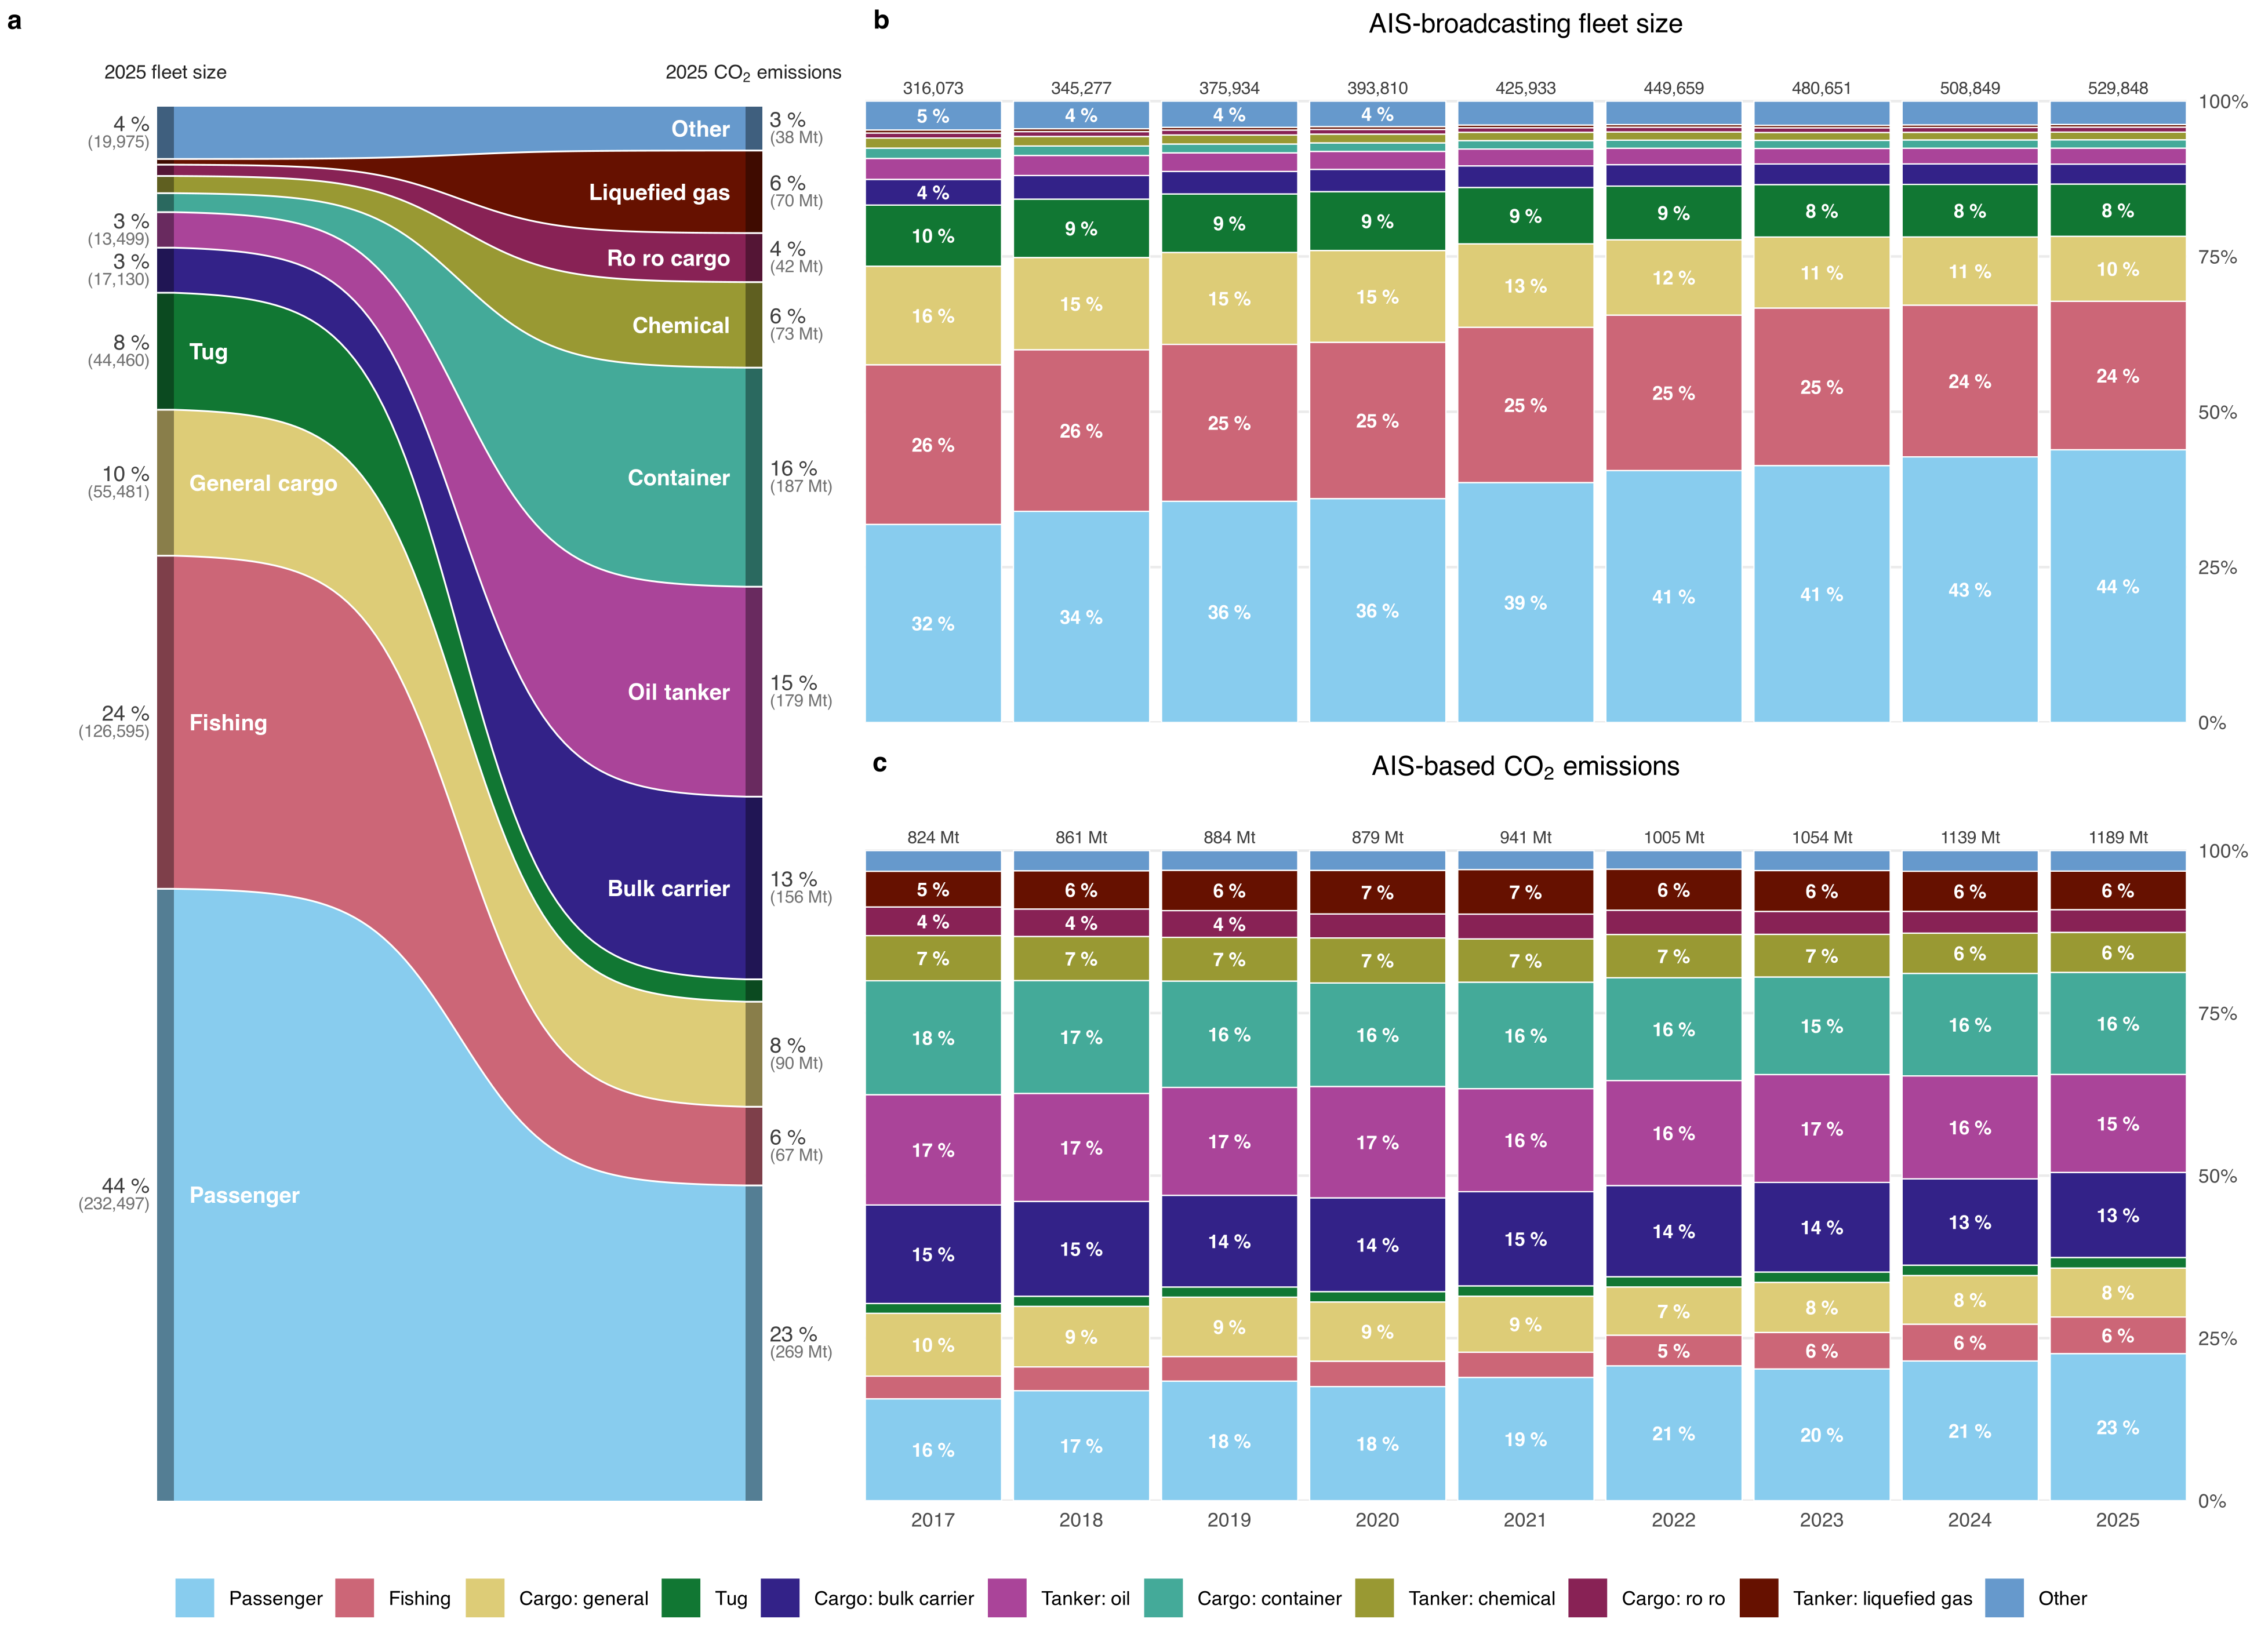
\includegraphics[width=\columnwidth]{figures/figS-fleet-sankey-with-series-2025-1.png}
    \caption{\DIFaddFL{Fleet composition in 2025: each vessel class's share of the fleet against its share of CO$_{2}$, with the supporting series.}}
    \label{fig:figS-fleet-sankey-with-series-2025}
\end{figure}

\section*{\DIFadd{Supplementary Tables}}

\DIFaddend \begin{table}[!h]
\centering
\DIFdelbeginFL %DIFDELCMD < \caption{%
{%DIFAUXCMD
%DIFDELCMD < \label{tab:total_percent_change_by_fleet}%%%
\DIFdelFL{Summary of 2017 and 2024 emissions, data source and pollutant.}}
%DIFAUXCMD
\DIFdelendFL \DIFaddbeginFL \caption{\label{tab:total_percent_change_by_fleet}\DIFaddFL{Summary of 2017 and 2025 emissions, data source and pollutant.}}
\DIFaddendFL \centering
\fontsize{6}{8}\selectfont
\DIFdelbeginFL %DIFDELCMD < \begin{tabular}[t]{l|l|l|l|l|l}
%DIFDELCMD < \hline
%DIFDELCMD < Source & Pollutant & 2017 emissions, MT & 2024 emissions, MT & Percent 2024 total & 2017 to 2024 change\\
%DIFDELCMD < \hline
%DIFDELCMD < AIS & CO2 & 8.47e+08 & 1.17e+09 & 85\% & 38\%\\
%DIFDELCMD < \hline
%DIFDELCMD < S1 & CO2 & 1.92e+08 & 2.09e+08 & 15\% & 9\%\\
%DIFDELCMD < \hline
%DIFDELCMD < AIS + S1 & CO2 & 1.04e+09 & 1.38e+09 & 100\% & 33\%\\
%DIFDELCMD < \hline
%DIFDELCMD < AIS & CH4 & 13,600 & 18,500 & 83\% & 36\%\\
%DIFDELCMD < \hline
%DIFDELCMD < S1 & CH4 & 3,310 & 3,670 & 17\% & 11\%\\
%DIFDELCMD < \hline
%DIFDELCMD < AIS + S1 & CH4 & 16,900 & 22,200 & 100\% & 31\%\\
%DIFDELCMD < \hline
%DIFDELCMD < AIS & N2O & 41,400 & 57,200 & 85\% & 38\%\\
%DIFDELCMD < \hline
%DIFDELCMD < S1 & N2O & 9,530 & 10,400 & 15\% & 9\%\\
%DIFDELCMD < \hline
%DIFDELCMD < AIS + S1 & N2O & 50,900 & 67,600 & 100\% & 33\%\\
%DIFDELCMD < \hline
%DIFDELCMD < AIS & CO & 681,000 & 920,000 & 84\% & 35\%\\
%DIFDELCMD < \hline
%DIFDELCMD < S1 & CO & 158,000 & 173,000 & 16\% & 10\%\\
%DIFDELCMD < \hline
%DIFDELCMD < AIS + S1 & CO & 838,000 & 1,090,000 & 100\% & 30\%\\
%DIFDELCMD < \hline
%DIFDELCMD < AIS & NOX & 14,500,000 & 19,200,000 & 85\% & 32\%\\
%DIFDELCMD < \hline
%DIFDELCMD < S1 & NOX & 3,240,000 & 3,500,000 & 15\% & 8\%\\
%DIFDELCMD < \hline
%DIFDELCMD < AIS + S1 & NOX & 17,800,000 & 22,700,000 & 100\% & 28\%\\
%DIFDELCMD < \hline
%DIFDELCMD < AIS & SOX & 5,240,000 & 1,440,000 & 85\% & -72\%\\
%DIFDELCMD < \hline
%DIFDELCMD < S1 & SOX & 1,190,000 & 258,000 & 15\% & -78\%\\
%DIFDELCMD < \hline
%DIFDELCMD < AIS + S1 & SOX & 6,420,000 & 1,700,000 & 100\% & -74\%\\
%DIFDELCMD < \hline
%DIFDELCMD < AIS & PM2.5 & 1,430,000 & 411,000 & 84\% & -71\%\\
%DIFDELCMD < \hline
%DIFDELCMD < S1 & PM2.5 & 335,000 & 75,900 & 16\% & -77\%\\
%DIFDELCMD < \hline
%DIFDELCMD < AIS + S1 & PM2.5 & 1,770,000 & 487,000 & 100\% & -72\%\\
%DIFDELCMD < \hline
%DIFDELCMD < AIS & PM10 & 1,560,000 & 447,000 & 84\% & -71\%\\
%DIFDELCMD < \hline
%DIFDELCMD < S1 & PM10 & 365,000 & 82,500 & 16\% & -77\%\\
%DIFDELCMD < \hline
%DIFDELCMD < AIS + S1 & PM10 & 1,920,000 & 529,000 & 100\% & -72\%\\
%DIFDELCMD < \hline
%DIFDELCMD < AIS & VOCs & 942,000 & 1,330,000 & 84\% & 41\%\\
%DIFDELCMD < \hline
%DIFDELCMD < S1 & VOCs & 233,000 & 260,000 & 16\% & 12\%\\
%DIFDELCMD < \hline
%DIFDELCMD < AIS + S1 & VOCs & 1,170,000 & 1,590,000 & 100\% & 35\%\\
%DIFDELCMD < \hline
%DIFDELCMD < \end{tabular}
%DIFDELCMD < %%%
\DIFdelendFL \DIFaddbeginFL \setlength{\tabcolsep}{3pt}
\begin{tabular}[t]{l|l|l|l|l|l}
\hline
Source & Pollutant & \shortstack{2017\\emissions, MT} & \shortstack{2025\\emissions, MT} & \shortstack{Percent 2025\\total} & \shortstack{2017 to 2025\\change}\\
\hline
AIS-based & CO2 & 8.24e+08 & 1.19e+09 & 82\% & 44\%\\
\hline
S1-unmatched & CO2 & 2.41e+08 & 2.54e+08 & 18\% & 5\%\\
\hline
AIS-based + S1-unmatched & CO2 & 1.06e+09 & 1.44e+09 & 100\% & 36\%\\
\hline
AIS-based & CH4 & 11,500 & 15,800 & 84\% & 37\%\\
\hline
S1-unmatched & CH4 & 2,880 & 2,960 & 16\% & 3\%\\
\hline
AIS-based + S1-unmatched & CH4 & 14,400 & 18,700 & 100\% & 30\%\\
\hline
AIS-based & N2O & 41,800 & 59,500 & 83\% & 42\%\\
\hline
S1-unmatched & N2O & 11,800 & 12,400 & 17\% & 5\%\\
\hline
AIS-based + S1-unmatched & N2O & 53,600 & 71,900 & 100\% & 34\%\\
\hline
AIS-based & CO & 628,000 & 865,000 & 84\% & 38\%\\
\hline
S1-unmatched & CO & 160,000 & 165,000 & 16\% & 3\%\\
\hline
AIS-based + S1-unmatched & CO & 787,000 & 1,030,000 & 100\% & 31\%\\
\hline
AIS-based & NOX & 14,100,000 & 18,500,000 & 85\% & 31\%\\
\hline
S1-unmatched & NOX & 3,320,000 & 3,320,000 & 15\% & 0\%\\
\hline
AIS-based + S1-unmatched & NOX & 17,400,000 & 21,800,000 & 100\% & 25\%\\
\hline
AIS-based & SOX & 5,030,000 & 1,830,000 & 82\% & -64\%\\
\hline
S1-unmatched & SOX & 1,490,000 & 390,000 & 18\% & -74\%\\
\hline
AIS-based + S1-unmatched & SOX & 6,510,000 & 2,220,000 & 100\% & -66\%\\
\hline
AIS-based & PM2.5 & 701,000 & 590,000 & 84\% & -16\%\\
\hline
S1-unmatched & PM2.5 & 192,000 & 113,000 & 16\% & -41\%\\
\hline
AIS-based + S1-unmatched & PM2.5 & 893,000 & 703,000 & 100\% & -21\%\\
\hline
AIS-based & PM10 & 762,000 & 641,000 & 84\% & -16\%\\
\hline
S1-unmatched & PM10 & 208,000 & 123,000 & 16\% & -41\%\\
\hline
AIS-based + S1-unmatched & PM10 & 970,000 & 764,000 & 100\% & -21\%\\
\hline
AIS-based & VOCs & 641,000 & 868,000 & 85\% & 35\%\\
\hline
S1-unmatched & VOCs & 154,000 & 157,000 & 15\% & 2\%\\
\hline
AIS-based + S1-unmatched & VOCs & 795,000 & 1,020,000 & 100\% & 29\%\\
\hline
\end{tabular}
\DIFaddendFL \end{table}
\DIFaddbegin \FloatBarrier
\DIFaddend 

\begin{table}[!h]
\centering
\DIFdelbeginFL %DIFDELCMD < \caption{%
{%DIFAUXCMD
%DIFDELCMD < \label{tab:pollutant_ais_underestimation_overestimation_summary}%%%
\DIFdelFL{Underestimation of 2024 emissions using only AIS data, and overestimation of 2017 to 2024 emissions trend using only AIS data, by pollutant.}}
%DIFAUXCMD
\DIFdelendFL \DIFaddbeginFL \caption{\label{tab:growth_share_by_family_length}\DIFaddFL{Share of the 2017--2025 growth in AIS-based CO$_{2}$ emissions contributed by each vessel class family and length band. Each cell is that group's change in emissions as a share of the total change of 365 million metric tonnes (from 824 to 1,189 million), so the cells sum to 100\%. Vessel class families are as in Fig. \ref{fig:fig-ais-data-richness}; passenger vessels account for 38 of the 44 percentage points of the service and passenger family. Moving the upper length cutoff from 150 m to 200 m would shift 6 percentage points from the largest band to the middle band and leave the $<$50 m share unchanged. Percentages may not sum to totals because of rounding.}}
\DIFaddendFL \centering
\DIFdelbeginFL %DIFDELCMD < \fontsize{8}{10}%%%
\DIFdelendFL \DIFaddbeginFL \fontsize{7}{9}\DIFaddendFL \selectfont
\DIFdelbeginFL %DIFDELCMD < \begin{tabular}[t]{l|l|l}
%DIFDELCMD < \hline
%DIFDELCMD < Pollutant & Underestimation of 2024 emissions & Overestimation of 2017-2024 emissions trend\\
%DIFDELCMD < \hline
%DIFDELCMD < CO2 & 15\% & 16\%\\
%DIFDELCMD < \hline
%DIFDELCMD < CH4 & 17\% & 16\%\\
%DIFDELCMD < \hline
%DIFDELCMD < N2O & 15\% & 16\%\\
%DIFDELCMD < \hline
%DIFDELCMD < CO & 16\% & 16\%\\
%DIFDELCMD < \hline
%DIFDELCMD < NOX & 15\% & 16\%\\
%DIFDELCMD < \hline
%DIFDELCMD < SOX & 15\% & -1\%\\
%DIFDELCMD < \hline
%DIFDELCMD < PM2.5 & 16\% & -2\%\\
%DIFDELCMD < \hline
%DIFDELCMD < PM10 & 16\% & -2\%\\
%DIFDELCMD < \hline
%DIFDELCMD < VOCs & 16\% & 17\%\\
%DIFDELCMD < \hline
%DIFDELCMD < \end{tabular}
%DIFDELCMD < %%%
\DIFdelendFL \DIFaddbeginFL \begin{tabular}[t]{lrrrr}
\toprule
Vessel class family & $<$50 m & 50--150 m & $\geq$150 m & Total\\
\midrule
Cargo & 1\% & 2\% & 20\% & 24\%\\
Tanker & $<$1\% & 3\% & 19\% & 22\%\\
Service and passenger & 39\% & 4\% & 1\% & 44\%\\
Fishing & 10\% & 1\% & $<$1\% & 10\%\\
\midrule
Total & 50\% & 10\% & 40\% & 100\%\\
\bottomrule
\end{tabular}
\DIFaddendFL \end{table}
\DIFaddbegin \FloatBarrier
\DIFaddend 

\begin{table}[!h]
\centering
\DIFdelbeginFL %DIFDELCMD < \caption{%
{%DIFAUXCMD
%DIFDELCMD < \label{tab:emissions_by_ocean_summary_tbl}%%%
\DIFdelFL{For each ocean, summary of: 2024 total (AIS+S1) CO$_2$ emissions (metric tonnes); percentage of global total (AIS+S1) 2024 CO$_2$ emissions from across all oceans; percent of 2024 total (AIS+S1) CO$_2$ emissions by non-broadcasting vessels; percent change in total (AIS+S1) CO$_2$ emissions from 2017 to 2024; and the percentage of all observations in the dataset (pixel-months) from 2017-2024 that were imaged by S1.}}
%DIFAUXCMD
\DIFdelendFL \DIFaddbeginFL \caption{\label{tab:growth_decomposition_by_family_length}\DIFaddFL{Decomposition of the 2017--2025 change in AIS-based CO$_{2}$ emissions in each vessel class family and length band of Supplementary Table \ref{tab:growth_share_by_family_length}, in million metric tonnes. A cell's emissions are the product of its vessel count, the distance each vessel traveled (nm per vessel), and its emissions per nautical mile. The log-mean Divisia index \mbox{%DIFAUXCMD
\cite{angLMDIApproachDecomposition2005} }\hskip0pt%DIFAUXCMD
splits the change in emissions exactly into a contribution from the change in each factor, so the three contributions in a row sum to its emissions change. Vessel count is the number of distinct AIS identities (MMSIs), so its change reflects fleet growth, the expansion of AIS carriage, and vessels changing MMSI. Among vessels of 150 m and over, MMSI changes make identities grow faster than physical hulls, so part of their vessel count contribution belongs to distance per vessel. Distance per vessel is observed distance, which also rises when improved AIS reception fills gaps in vessel tracks. Emissions per nautical mile include auxiliary engine and at-berth emissions, which accrue with time rather than distance, so this factor is not a measure of fuel efficiency alone.}}
\DIFaddendFL \centering
\DIFdelbeginFL %DIFDELCMD < \begin{tabular}[t]{l|l|l|l|l|l}
%DIFDELCMD < \hline
%DIFDELCMD < Summary statistic & Indian & Pacific & Arctic & Southern & Atlantic\\
%DIFDELCMD < \hline
%DIFDELCMD < 2024 total CO2 emissions (million MT) & 224 & 452 & 4.65 & 0.607 & 441\\
%DIFDELCMD < \hline
%DIFDELCMD < Percent of total CO2 2024 emissions & 19.65\% & 40.99\% & 0.42\% & 0.05\% & 38.89\%\\
%DIFDELCMD < \hline
%DIFDELCMD < Percent of total CO2 emissions by non-broadcasting & 14.49\% & 17.09\% & 16.84\% & 1.76\% & 14.81\%\\
%DIFDELCMD < \hline
%DIFDELCMD < Percent change in total CO2 emissions (2017 to 2024) & 25.31\% & 43.03\% & 18.24\% & 269.44\% & 28.09\%\\
%DIFDELCMD < \hline
%DIFDELCMD < Percent observations imaged by S1 (across 2017-2024) & 17.12\% & 17.91\% & 14.45\% & 0.07\% & 36.31\%\\
%DIFDELCMD < \hline
%DIFDELCMD < \end{tabular}
%DIFDELCMD < %%%
\DIFdelendFL \DIFaddbeginFL \fontsize{7}{9}\selectfont
\setlength{\tabcolsep}{3pt}
\begin{tabular}[t]{llrrrr}
\toprule
\multicolumn{3}{c}{ } & \multicolumn{3}{c}{Contribution from change in:} \\
\cmidrule(l{3pt}r{3pt}){4-6}
Vessel class family & Length & \shortstack{Emissions\\change} & \shortstack{Vessel\\count} & \shortstack{nm per\\vessel} & \shortstack{CO$_{2}$\\per nm}\\
\midrule
Cargo & $<$50 m & +3.9 & +1.4 & +0.2 & +2.3\\
 & 50--150 m & +8.8 & +11.5 & -7.0 & +4.4\\
 & $\geq$150 m & +74.3 & +86.9 & +4.0 & -16.7\\
\addlinespace
Tanker & $<$50 m & +0.9 & +0.4 & -0.2 & +0.7\\
 & 50--150 m & +10.8 & +7.9 & -5.1 & +8.0\\
 & $\geq$150 m & +68.9 & +94.1 & -21.1 & -4.1\\
\addlinespace
Service and passenger & $<$50 m & +142.2 & +126.3 & -23.3 & +39.2\\
 & 50--150 m & +14.1 & +10.9 & -0.8 & +4.0\\
 & $\geq$150 m & +3.1 & +6.4 & -3.5 & +0.2\\
\addlinespace
Fishing & $<$50 m & +35.0 & +15.3 & +13.5 & +6.2\\
 & 50--150 m & +3.2 & +0.3 & +0.8 & +2.1\\
 & $\geq$150 m & 0.0 & 0.0 & 0.0 & 0.0\\
\bottomrule
\end{tabular}
\DIFaddendFL \end{table}
\DIFaddbegin \FloatBarrier
\DIFaddend 

\begin{table}[!h]
\centering
\DIFdelbeginFL %DIFDELCMD < \caption{%
{%DIFAUXCMD
%DIFDELCMD < \label{tab:emissions_by_data_source_summary_tbl}%%%
\DIFdelFL{For each data source, summary of: total 2024 CO$_2$ emissions (metric tonnes); and percent change in CO$_2$ emissions from 2017 to 2024.}}
%DIFAUXCMD
\DIFdelendFL \DIFaddbeginFL \caption{\label{tab:pollutant_ais_underestimation_overestimation_summary}\DIFaddFL{Underestimation of 2025 emissions using only AIS data, and overestimation of the 2017 to 2025 percent change in emissions using only AIS data, by pollutant. Overestimation is the AIS-based percent change minus the AIS-based + S1-unmatched percent change, in percentage points; positive values mean AIS data alone show faster growth, or a slower decline, than the fused estimate.}}
\DIFaddendFL \centering
\fontsize{8}{10}\selectfont
\DIFdelbeginFL %DIFDELCMD < \begin{tabular}[t]{l|l|l}
%DIFDELCMD < \hline
%DIFDELCMD < Data source & 2024 emissions, billion MT & Change in emissions, 2017 to 2024\\
%DIFDELCMD < \hline
%DIFDELCMD < Other transportation sectors (EDGAR) & 7.44 & 3.35\%\\
%DIFDELCMD < \hline
%DIFDELCMD < All sectors (EDGAR) & 39.6 & 7.06\%\\
%DIFDELCMD < \hline
%DIFDELCMD < Marine vessels (AIS + S1) & 1.38 & 32.56\%\\
%DIFDELCMD < \hline
%DIFDELCMD < \end{tabular}
%DIFDELCMD < %%%
\DIFdelendFL \DIFaddbeginFL \begin{tabular}[t]{l|l|l}
\hline
Pollutant & \shortstack{Underestimation of\\2025 emissions} & \shortstack{Overestimation of 2017-2025\\percent change (percentage points)}\\
\hline
CO2 & 18\% & 8.8\\
\hline
CH4 & 16\% & 7.0\\
\hline
N2O & 17\% & 8.3\\
\hline
CO & 16\% & 7.0\\
\hline
NOX & 15\% & 5.9\\
\hline
SOX & 18\% & 2.3\\
\hline
PM2.5 & 16\% & 5.4\\
\hline
PM10 & 16\% & 5.4\\
\hline
VOCs & 15\% & 6.5\\
\hline
\end{tabular}
\DIFaddendFL \end{table}
\DIFaddbegin \FloatBarrier
\DIFaddend 

\begin{table}[!h]
\centering
\DIFdelbeginFL %DIFDELCMD < \caption{%
{%DIFAUXCMD
%DIFDELCMD < \label{tab:social_cost_summary_tbl}%%%
\DIFdelFL{For both non-fishing vessels and fishing vessels, we summarize: the total emissions (metric tonnes) of each GHG gas; the social cost associated with each GHG (USD/metric tonne); the social cost of each (USD); the total social cost summed across all three gasses (USD). We use 2021 for non-fishing vessels since it is the year for which we have the total value of all traded goods at sea. We use 2022 for fishing vessels since it is the year for which we have the total value of wild capture fisheries.}}
%DIFAUXCMD
\DIFdelendFL \DIFaddbeginFL \caption{\label{tab:emissions_by_ocean_summary_tbl}\DIFaddFL{For each ocean, summary of: 2025 total (AIS+S1) CO$_2$ emissions (metric tonnes); percentage of global total (AIS+S1) 2025 CO$_2$ emissions from across all oceans; percent of 2025 total (AIS+S1) CO$_2$ emissions that are S1-unmatched; percent change in total (AIS+S1) CO$_2$ emissions from 2017 to 2025; and the percentage of all observations in the dataset (pixel-months) from 2017-2025 that were imaged by S1.}}
\DIFaddendFL \centering
\DIFdelbeginFL %DIFDELCMD < \fontsize{8}{10}%%%
\DIFdelendFL \DIFaddbeginFL \fontsize{7}{9}\DIFaddendFL \selectfont
\DIFdelbeginFL %DIFDELCMD < \begin{tabular}[t]{l|l|l|l|l|r}
%DIFDELCMD < \hline
%DIFDELCMD < Year & Vessel type & GHG & Emissions (MT) & SC (USD/MT) & SC (billion USD)\\
%DIFDELCMD < \hline
%DIFDELCMD < 2021 & Non-fishing & CH4 & 17,634 & 2,900 & 0.051\\
%DIFDELCMD < \hline
%DIFDELCMD < 2021 & Non-fishing & CO2 & 1,114,865,471 & 283 & 315.507\\
%DIFDELCMD < \hline
%DIFDELCMD < 2021 & Non-fishing & N2O & 54,576 & 49,600 & 2.707\\
%DIFDELCMD < \hline
%DIFDELCMD < Total & Non-fishing & - & - & - & 318.265\\
%DIFDELCMD < \hline
%DIFDELCMD < 2022 & Fishing & CH4 & 1,522 & 2,900 & 0.004\\
%DIFDELCMD < \hline
%DIFDELCMD < 2022 & Fishing & CO2 & 78,769,964 & 283 & 22.292\\
%DIFDELCMD < \hline
%DIFDELCMD < 2022 & Fishing & N2O & 3,953 & 49,600 & 0.196\\
%DIFDELCMD < \hline
%DIFDELCMD < Total & Fishing & - & - & - & 22.492\\
%DIFDELCMD < \hline
%DIFDELCMD < \end{tabular}
%DIFDELCMD < %%%
\DIFdelendFL \DIFaddbeginFL \setlength{\tabcolsep}{3pt}
\begin{tabular}[t]{l|l|l|l|l|l}
\hline
Summary statistic & Pacific & Atlantic & Indian & Arctic & Southern\\
\hline
2025 total CO2 emissions (million MT) & 457 & 449 & 222 & 4.13 & 0.567\\
\hline
Percent of total CO2 2025 emissions & 41.59\% & 38.98\% & 19.07\% & 0.32\% & 0.04\%\\
\hline
Percent of total CO2 emissions S1-unmatched & 20.59\% & 16.88\% & 16.10\% & 7.75\% & 0.00\%\\
\hline
Percent change in total CO2 emissions (2017 to 2025) & 44.24\% & 32.00\% & 28.49\% & 44.15\% & 263.43\%\\
\hline
Percent observations imaged by S1 (across 2017-2025) & 17.74\% & 35.94\% & 16.99\% & 13.55\% & 0.06\%\\
\hline
\end{tabular}
\DIFaddendFL \end{table}
\DIFaddbegin \FloatBarrier
\DIFaddend 

\DIFdelbegin \subsection{\DIFdel{Comparing our emission estimates to other inventories}}
%DIFAUXCMD
\addtocounter{subsection}{-1}%DIFAUXCMD
%DIFDELCMD < 

%DIFDELCMD < %%%
\DIFdel{Our total emissions estimates (summed across broadcasting and non-broadcasting vessels)
    are consistent with other well-known global inventories: the International Maritime Organization (IMO)
    \mbox{%DIFAUXCMD
\cite{fourth2020greenhouse}}\hskip0pt%DIFAUXCMD
, the EU's Emissions Database for Global Atmospheric Research (EDGAR)
    \mbox{%DIFAUXCMD
\cite{JRC143227}}\hskip0pt%DIFAUXCMD
, and the Organization for Economic Co-operation and Development (OECD)
    experimental shipping database \mbox{%DIFAUXCMD
\cite{clarke2023co2} }\hskip0pt%DIFAUXCMD
(Fig.\ref{fig:fig-inventory-comparison} and Table \ref{tab:inventory_comparison})
    . For each inventory, we pull all available years of data from 2017 through 2024. Both the IMO and OECD inventories leverage AIS data, with IMO using an AIS-based model similar to ours, and OECD leveraging a machine learning model trained on the EU MRV database that uses AIS movement data to inform certain model features and which uses this model to make predictions for AIS-broadcasting vessels not contained in the EU MRV database.The EDGAR inventory uses national fuel use data and regional emissionsfactors to estimate emissions . Our approach combining AIS and S1 data yields the highest estimates, as expected. The level of general agreement for this complex estimate across multiple sourcesprovides support for the reliability and utility of our methodology and results.
    }%DIFDELCMD < 

%DIFDELCMD < \begin{figure}[H]
%DIFDELCMD <     %%%
\DIFdelendFL \DIFaddbeginFL \begin{table}[!h]
\DIFaddendFL \centering
\DIFdelbeginFL %DIFDELCMD < 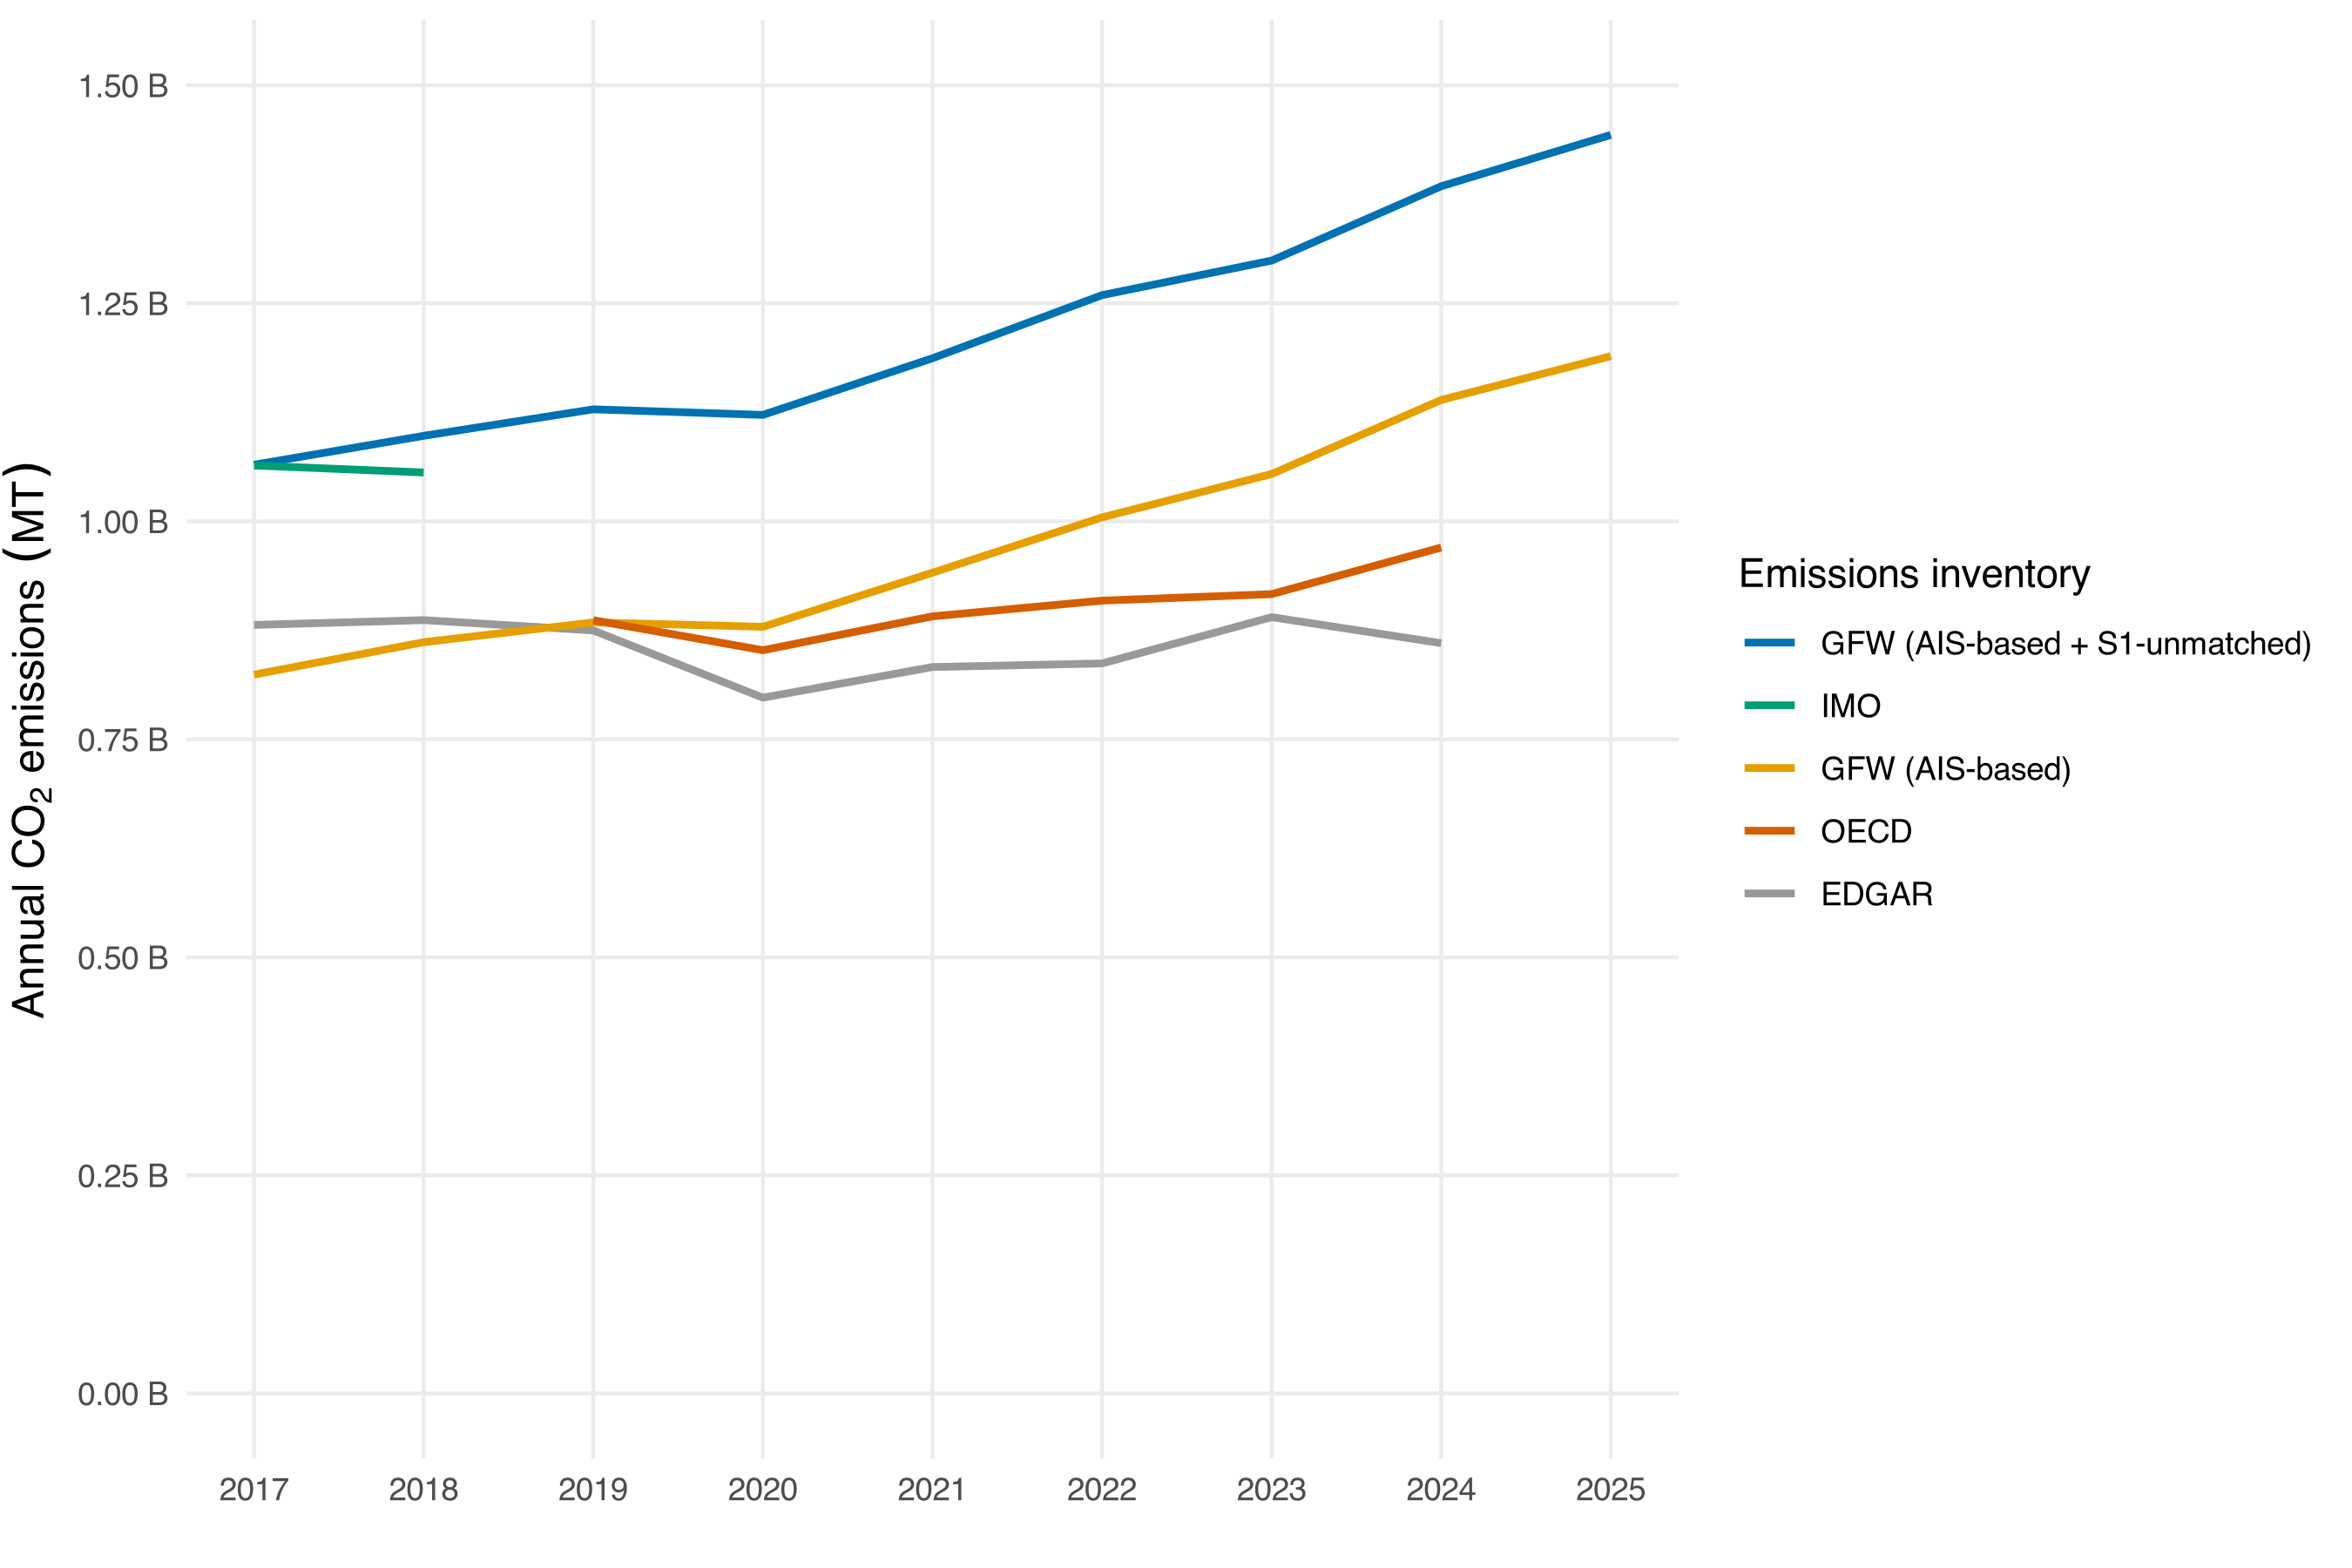
\includegraphics[width=\columnwidth]{figures/fig-inventory-comparison-1.png}
%DIFDELCMD <     \caption{%%%
\DIFdelFL{Comparison of annual marine vessel CO$_{2}$ emissions inventory estimates.}%DIFDELCMD < \MBLOCKRIGHTBRACE
%DIFDELCMD <     \label{fig:fig-inventory-comparison}
%DIFDELCMD < \end{figure}
%DIFDELCMD < %%%
\DIFdelend \DIFaddbegin \caption{\label{tab:social_cost_summary_tbl}\DIFadd{For both non-fishing vessels and fishing vessels, we summarize: the total emissions (metric tonnes) of each GHG gas; the social cost associated with each GHG (USD/metric tonne); the social cost of each (USD); the total social cost summed across all three gases (USD). We use 2021 for non-fishing vessels since it is the year for which we have the total value of all traded goods at sea. We use 2022 for fishing vessels since it is the year for which we have the total value of wild capture fisheries.}}
\centering
\fontsize{8}{10}\selectfont
\begin{tabular}[t]{l|l|l|l|l|r}
\hline
Year & Vessel type & GHG & Emissions (MT) & SC (USD/MT) & SC (billion USD)\\
\hline
2021 & Non-fishing & CH4 & 14,394 & 2,900 & 0.042\\
\hline
2021 & Non-fishing & CO2 & 1,126,390,708 & 283 & 318.769\\
\hline
2021 & Non-fishing & N2O & 56,293 & 49,600 & 2.792\\
\hline
Total & Non-fishing & - & - & - & 321.602\\
\hline
2022 & Fishing & CH4 & 1,344 & 2,900 & 0.004\\
\hline
2022 & Fishing & CO2 & 80,935,299 & 283 & 22.905\\
\hline
2022 & Fishing & N2O & 4,123 & 49,600 & 0.205\\
\hline
Total & Fishing & - & - & - & 23.113\\
\hline
\end{tabular}
\end{table}
\FloatBarrier
\DIFaddend 

\begin{table}[!h]
\centering
\DIFdelbeginFL %DIFDELCMD < \caption{\label{tab:inventory_comparison}%%%
\DIFdelFL{Comparison of annual marine vessel CO$_{2}$ emissions inventory estimates (billions of metric tonnes).}%DIFDELCMD < \MBLOCKRIGHTBRACE
%DIFDELCMD < %%%
\DIFdelendFL \DIFaddbeginFL \caption{\label{tab:top_countries_by_activity_type}\DIFaddFL{Top 30 countries by 2025 CO$_{2}$ emissions (millions of metric tonnes) from AIS-broadcasting vessels, shown separately for each activity type, with all remaining countries pooled into a single Other row. Emissions for each international trip are partitioned equally to its departure and arrival country. These are the totals mapped in Figure \ref{fig:fig-emissions-by-country-and-activity-type}.}}
\DIFaddendFL \centering
\DIFdelbeginFL %DIFDELCMD < \fontsize{8}{10}%%%
\DIFdelendFL \DIFaddbeginFL \fontsize{7}{9}\DIFaddendFL \selectfont
\DIFdelbeginFL %DIFDELCMD < \begin{tabular}[t]{r|l|l|l|l|l}
%DIFDELCMD < \hline
%DIFDELCMD < Year & GFW (AIS + S1) & GFW (AIS) & EDGAR & OECD & IMO\\
%DIFDELCMD < \hline
%DIFDELCMD < 2017 & 1.04 & 0.847 & 0.881 & - & 1.06\\
%DIFDELCMD < \hline
%DIFDELCMD < 2018 & 1.07 & 0.877 & 0.887 & - & 1.06\\
%DIFDELCMD < \hline
%DIFDELCMD < 2019 & 1.1 & 0.899 & 0.875 & 0.887 & -\\
%DIFDELCMD < \hline
%DIFDELCMD < 2020 & 1.1 & 0.889 & 0.798 & 0.852 & -\\
%DIFDELCMD < \hline
%DIFDELCMD < 2021 & 1.17 & 0.966 & 0.833 & 0.891 & -\\
%DIFDELCMD < \hline
%DIFDELCMD < 2022 & 1.25 & 1.04 & 0.837 & 0.909 & -\\
%DIFDELCMD < \hline
%DIFDELCMD < 2023 & 1.29 & 1.09 & 0.89 & 0.917 & -\\
%DIFDELCMD < \hline
%DIFDELCMD < 2024 & 1.38 & 1.17 & 0.86 & 0.97 & -\\
%DIFDELCMD < \hline
%DIFDELCMD < \end{tabular}
%DIFDELCMD < %%%
\DIFdelendFL \DIFaddbeginFL \begin{tabular}[t]{lrlrlr}
\toprule
\multicolumn{2}{c}{International trips} & \multicolumn{2}{c}{Port stays} & \multicolumn{2}{c}{Domestic trips} \\
\cmidrule(l{3pt}r{3pt}){1-2} \cmidrule(l{3pt}r{3pt}){3-4} \cmidrule(l{3pt}r{3pt}){5-6}
Country & CO$_{2}$ & Country & CO$_{2}$ & Country & CO$_{2}$\\
\midrule
China & 55.5 & China & 74.2 & China & 66.8\\
Malaysia & 48.1 & United States & 27.9 & Japan & 13.1\\
United States & 39.9 & Indonesia & 10.6 & United States & 13.1\\
South Korea & 20.2 & Spain & 9.8 & Indonesia & 8.8\\
Australia & 19.1 & South Korea & 9.0 & South Korea & 5.7\\
\addlinespace
Brazil & 18.9 & Netherlands & 9.0 & Russia & 5.6\\
Spain & 15.7 & Japan & 8.9 & Norway & 5.4\\
Japan & 15.5 & United Arab Emirates & 8.4 & Brazil & 5.2\\
India & 15.2 & Norway & 8.4 & Australia & 3.8\\
United Arab Emirates & 14.2 & Italy & 8.1 & Malaysia & 3.4\\
\addlinespace
Panama & 13.8 & Australia & 7.6 & India & 3.4\\
Singapore & 12.7 & Turkey & 7.4 & Italy & 3.2\\
Egypt & 10.4 & France & 7.2 & Spain & 3.1\\
Indonesia & 9.0 & United Kingdom & 6.7 & Turkey & 2.7\\
Russia & 8.5 & Germany & 6.0 & United Kingdom & 2.6\\
\addlinespace
United Kingdom & 7.7 & Greece & 5.8 & Canada & 2.5\\
Netherlands & 7.4 & Brazil & 5.3 & Vietnam & 2.3\\
Canada & 6.9 & Russia & 5.0 & United Arab Emirates & 2.2\\
Mexico & 6.4 & India & 4.8 & Philippines & 2.2\\
Turkey & 6.3 & Malaysia & 4.7 & Greece & 1.8\\
\addlinespace
Taiwan & 6.1 & Canada & 4.5 & Taiwan & 1.8\\
Belgium & 6.0 & Denmark & 4.4 & France & 1.7\\
France & 5.6 & Belgium & 3.9 & Egypt & 1.7\\
Saudi Arabia & 5.5 & Saudi Arabia & 3.3 & Saudi Arabia & 1.6\\
South Africa & 5.5 & Mexico & 2.8 & Mexico & 1.3\\
\addlinespace
Vietnam & 5.4 & Thailand & 2.8 & Germany & 1.1\\
Italy & 5.0 & Sweden & 2.5 & Chile & 1.1\\
Germany & 5.0 & Philippines & 2.3 & Thailand & 1.1\\
Sri Lanka & 4.9 & Taiwan & 2.2 & New Zealand & 1.0\\
Morocco & 4.7 & Egypt & 2.2 & Argentina & 1.0\\
\addlinespace
Other & 107.2 & Other & 59.3 & Other & 19.5\\
\bottomrule
\end{tabular}
\DIFaddendFL \end{table}
\DIFaddbegin \FloatBarrier
\DIFaddend 


\DIFdelbegin \subsection{\DIFdel{Trends in AIS receiver types}}
%DIFAUXCMD
\addtocounter{subsection}{-1}%DIFAUXCMD
\DIFdelend \DIFaddbegin \section*{\DIFadd{Supplementary Notes}}
\DIFaddend 

\DIFaddbegin \supnote{Trends in AIS receiver types}{sec:ais-receiver-types}

\DIFaddend AIS messages are broadcast from vessels and then received through one of three technologies: satellite-based receivers, terrestrial receivers, and dynamic receivers. Satellite and terrestrial receivers are the oldest receiver types, while 2022 saw the widespread adoption of \DIFdelbegin \DIFdel{'Dynamic-AIS' }\DIFdelend \DIFaddbegin \DIFadd{dynamic AIS (D-AIS) }\DIFaddend in several regions throughout the world. \DIFdelbegin \DIFdel{Dynamic AIS }\DIFdelend \DIFaddbegin \DIFadd{D-AIS }\DIFaddend is a technology that was first implemented by Spire, one of the major AIS data providers, in which satellite-enabled AIS receivers are installed on vessels that travel through some of the world's busiest shipping lanes, such as the South China Sea \cite{spire_documentation_2022}. Through GFW, we can determine the receiver type for every single AIS message in the dataset over time. In \DIFaddbegin \DIFadd{Supplementary }\DIFaddend Fig. \ref{fig:fig-annual-emissions-by-ais-receiver-type}, we summarize the amount of estimated emissions and the number of distinct vessels that were detected by the three different types of AIS receivers. In 2022, we can clearly see a sharp rise in the amount of emissions that were estimated from \DIFdelbegin \DIFdel{Dynamic AIS}\DIFdelend \DIFaddbegin \DIFadd{D-AIS}\DIFaddend , which intuitively coincides with a decrease in the emissions that are estimated from satellite and terrestrial receivers. On aggregate, this led to an increase in total estimated emissions. The number of distinct vessels detected by \DIFdelbegin \DIFdel{dynamic AIS }\DIFdelend \DIFaddbegin \DIFadd{D-AIS }\DIFaddend also sharply rose in 2022, almost equaling the number of vessels detected by all receiver types.

\begin{figure}[H]
    \centering
    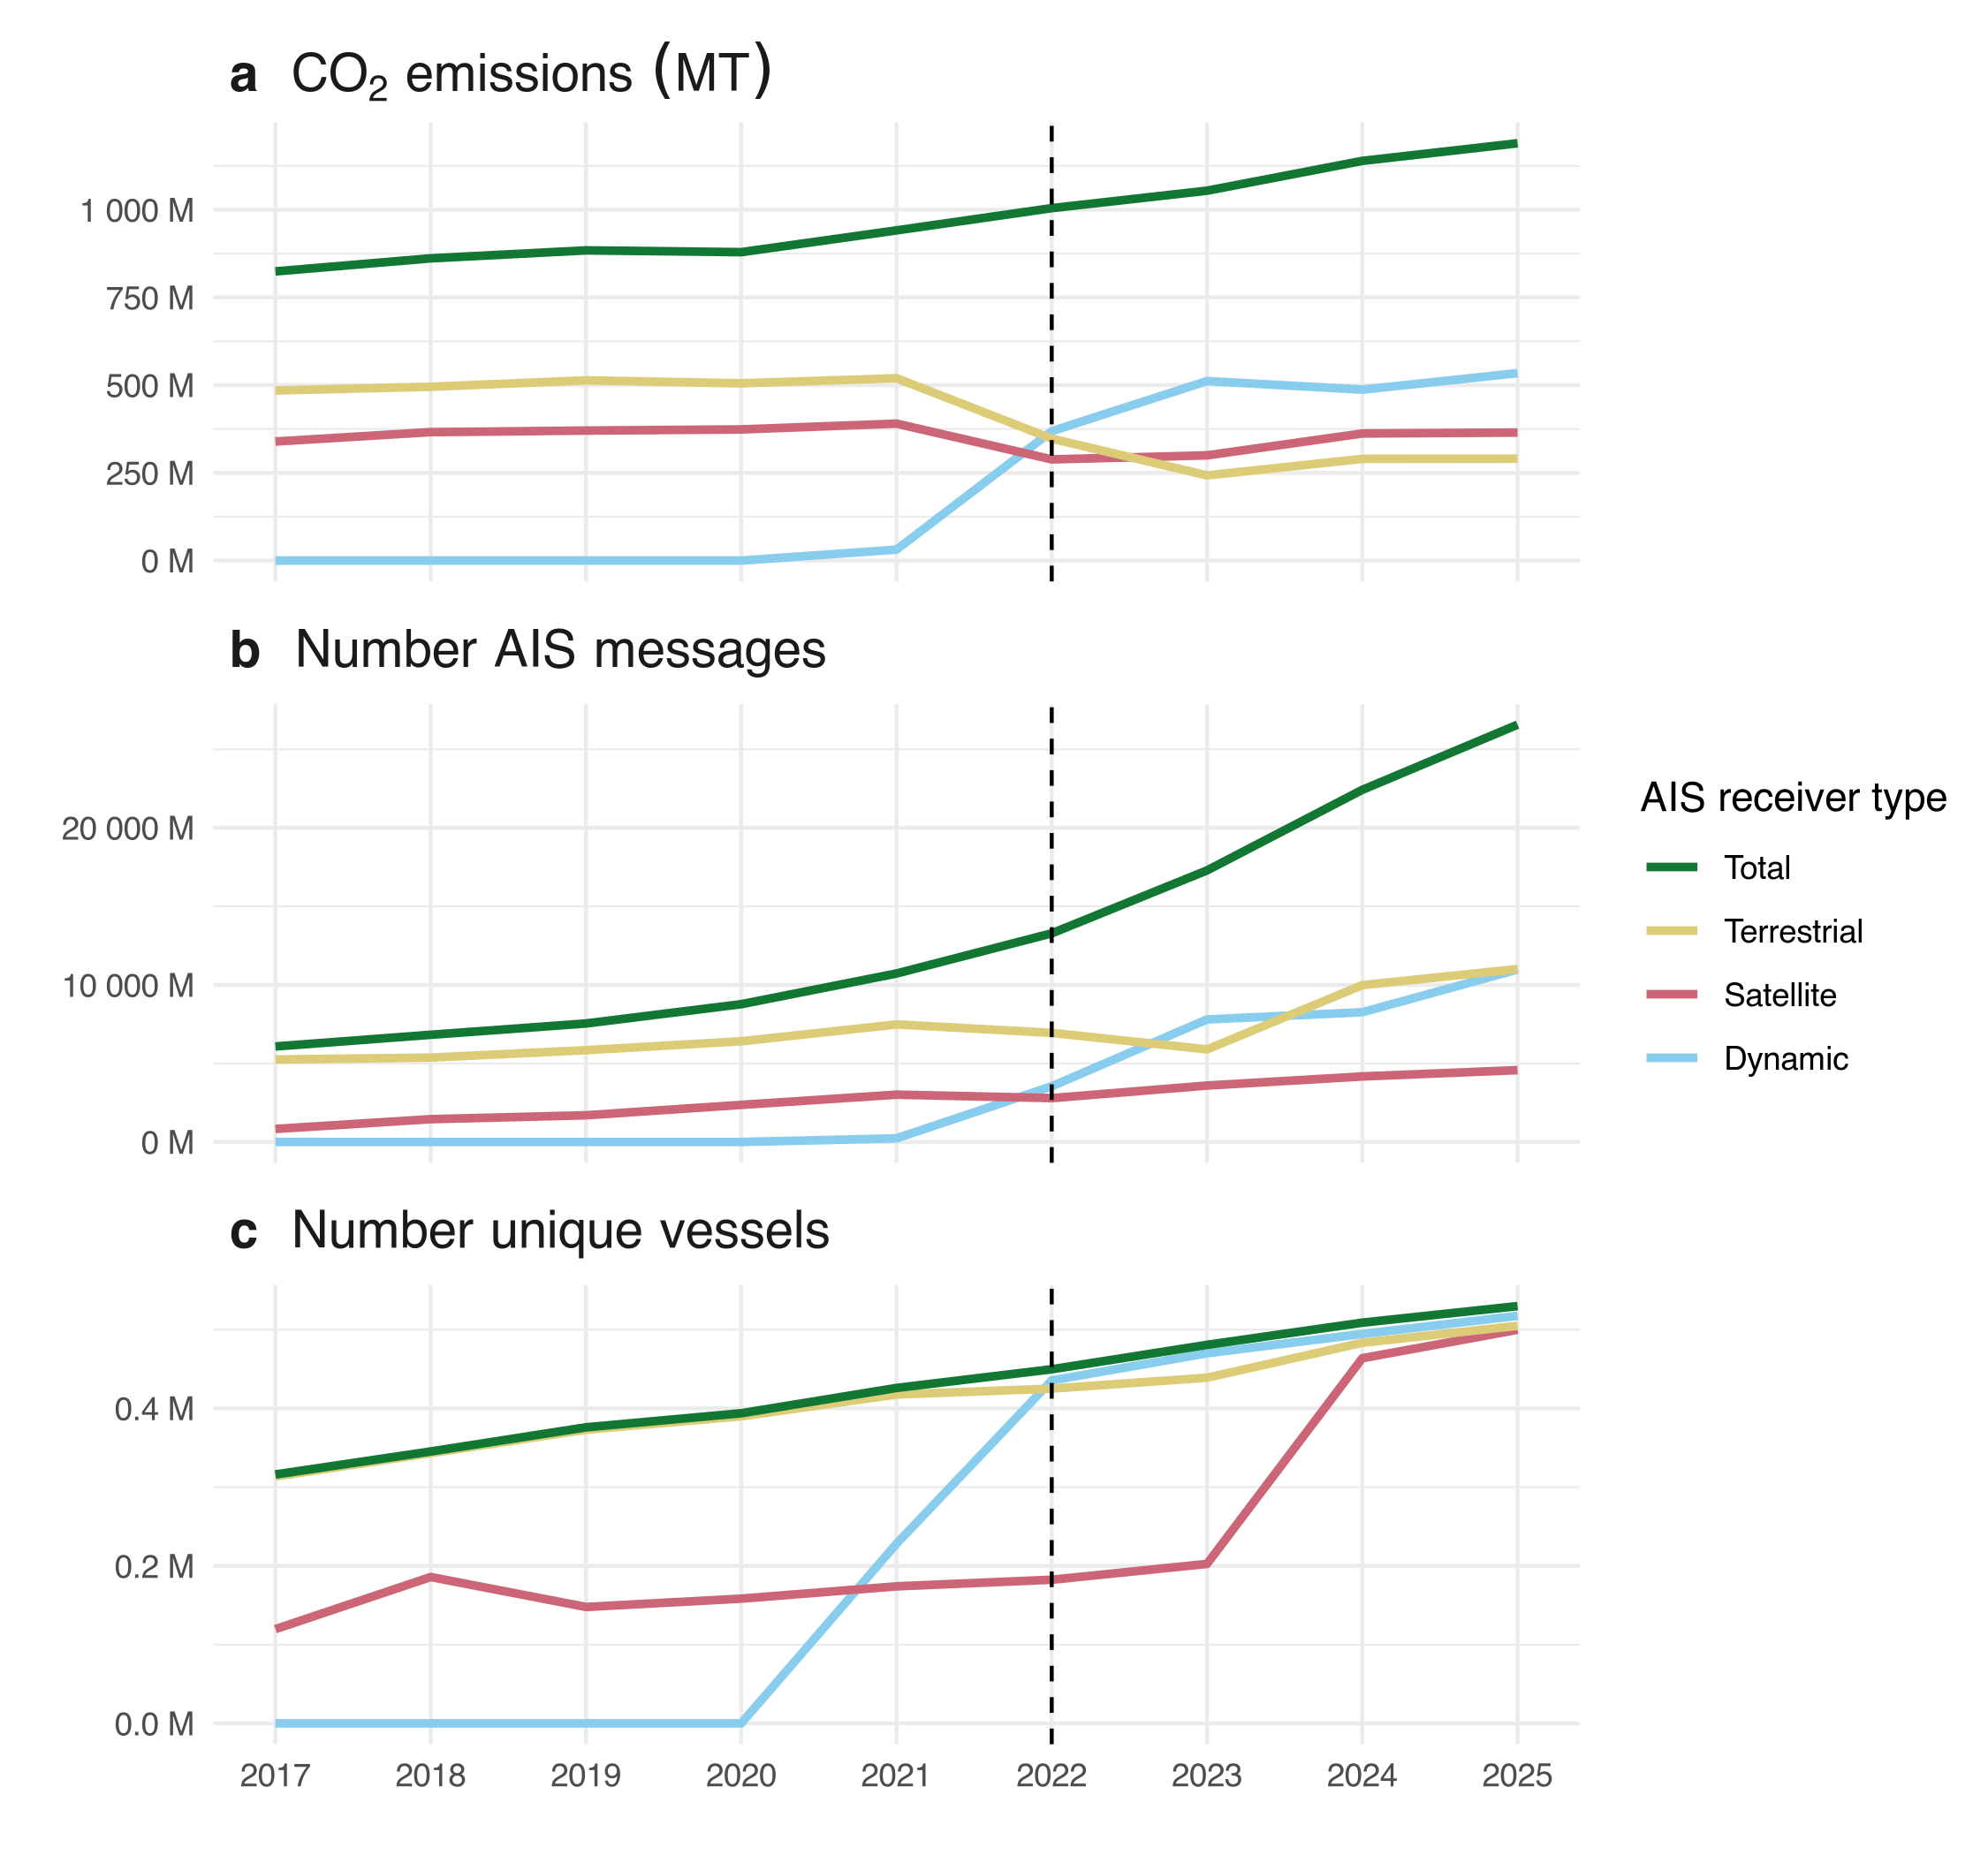
\includegraphics[width=\columnwidth]{figures/fig-annual-emissions-by-ais-receiver-type-1.png}
    \caption{\DIFaddbeginFL \DIFaddFL{(a) }\DIFaddendFL Annual total CO$_{2}$ emissions (metric tonnes) by AIS-broadcasting vessels, \DIFaddbeginFL \DIFaddFL{(b) }\DIFaddendFL AIS pings (i.e., individual vessel timestamped location messages), and \DIFaddbeginFL \DIFaddFL{(c) }\DIFaddendFL number of unique AIS-broadcasting vessels. Trends are disaggregated by AIS receiver type (satellite, terrestrial, and dynamic), and also shown as a total aggregated across receiver types. A dashed vertical line is shown for 2022, the first year in which \DIFdelbeginFL \DIFdelFL{dynamic AIS }\DIFdelendFL \DIFaddbeginFL \DIFaddFL{D-AIS }\DIFaddendFL was widely adopted.}
    \label{fig:fig-annual-emissions-by-ais-receiver-type}
\end{figure}

In \DIFaddbegin \DIFadd{Supplementary }\DIFaddend Fig. \ref{fig:fig-annual-emissions-by-ais-receiver-type-top-flags}, we see the amount of quantified emissions for the top 10 vessel flags broken apart by AIS receiver type. The trends are similar to those seen on aggregate (\DIFaddbegin \DIFadd{Supplementary }\DIFaddend Fig. \ref{fig:fig-annual-emissions-by-ais-receiver-type}), although there is variation in terms of the increase in \DIFdelbegin \DIFdel{Dynamic AIS }\DIFdelend \DIFaddbegin \DIFadd{D-AIS }\DIFaddend detections across different flags. This is likely driven by whether or not each flag travels through regions where \DIFdelbegin \DIFdel{Dynamic AIS }\DIFdelend \DIFaddbegin \DIFadd{D-AIS }\DIFaddend was widely adopted. It is important to note that towards the end of 2021, China experience\DIFaddbegin \DIFadd{d}\DIFaddend  a blackout of terrestrial AIS signals due to new privacy laws that were being implemented \cite{benefits_dynamic_ais}.

\begin{figure}[H]
    \centering
    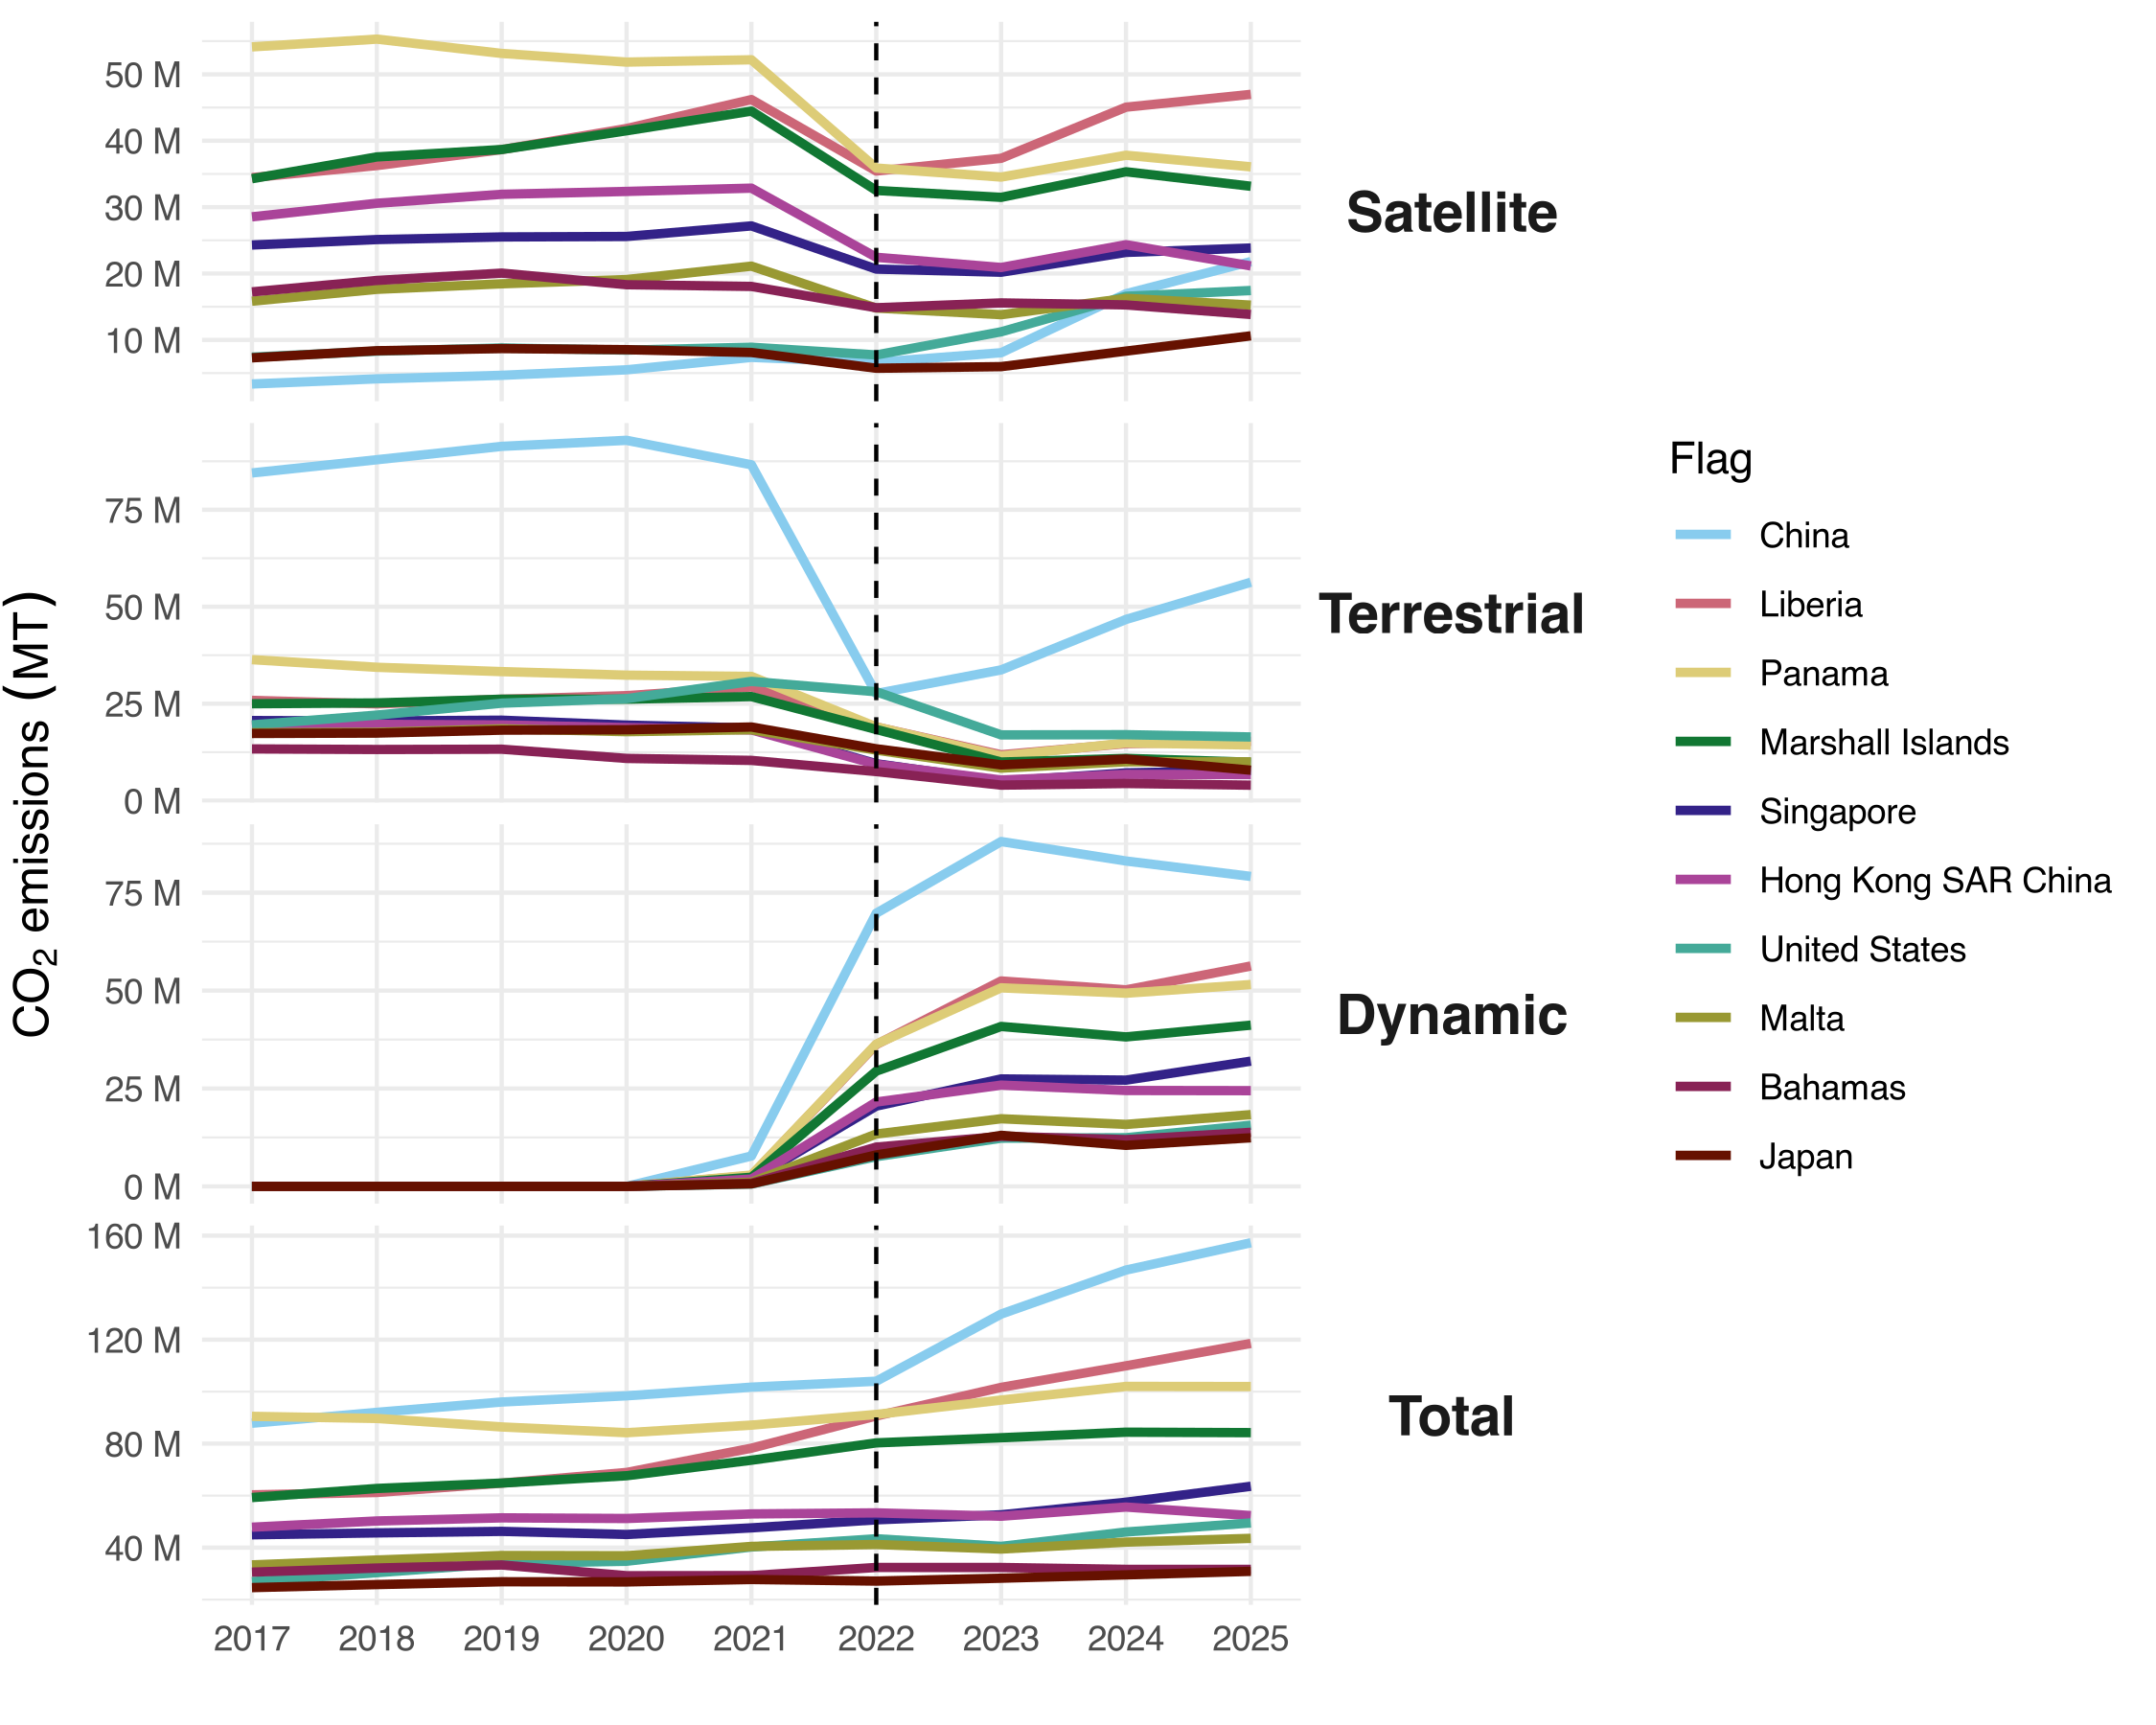
\includegraphics[width=\columnwidth]{figures/fig-annual-emissions-by-ais-receiver-type-top-flags-1.png}
    \caption{Annual total CO$_{2}$ emissions (metric tonnes) by AIS-broadcasting vessels, disaggregated by AIS receiver type (satellite, terrestrial, and dynamic) and total aggregated across receiver types, for the top 10 flags with the most emissions in \DIFdelbeginFL \DIFdelFL{2024. }\DIFdelendFL \DIFaddbeginFL \DIFaddFL{2025. }\DIFaddendFL A dashed vertical line is shown for 2022, the first year in which \DIFdelbeginFL \DIFdelFL{dynamic AIS }\DIFdelendFL \DIFaddbeginFL \DIFaddFL{D-AIS }\DIFaddendFL was widely adopted.}
    \label{fig:fig-annual-emissions-by-ais-receiver-type-top-flags}
\end{figure}

Finally, in \DIFaddbegin \DIFadd{Supplementary }\DIFaddend Fig. \ref{fig:fig-co2-emissions-change-map-by-receiver-type}, we see how the use of the three AIS receiver types has changed spatially over time between 2017 and \DIFdelbegin \DIFdel{2024. Dynamic AIS }\DIFdelend \DIFaddbegin \DIFadd{2025. D-AIS }\DIFaddend was mostly implemented in busy shipping lanes, with clear concentration in areas including the South China Sea, Europe, and the Gulf of Mexico. These regions also generally correspond to decreasing use of satellite and terrestrial receivers. Overall, the largest total change in emissions is generally concentrated in the same regions that saw the largest uptake of \DIFdelbegin \DIFdel{Dynamic AIS}\DIFdelend \DIFaddbegin \DIFadd{D-AIS}\DIFaddend .

\begin{figure}[H]
    \centering
    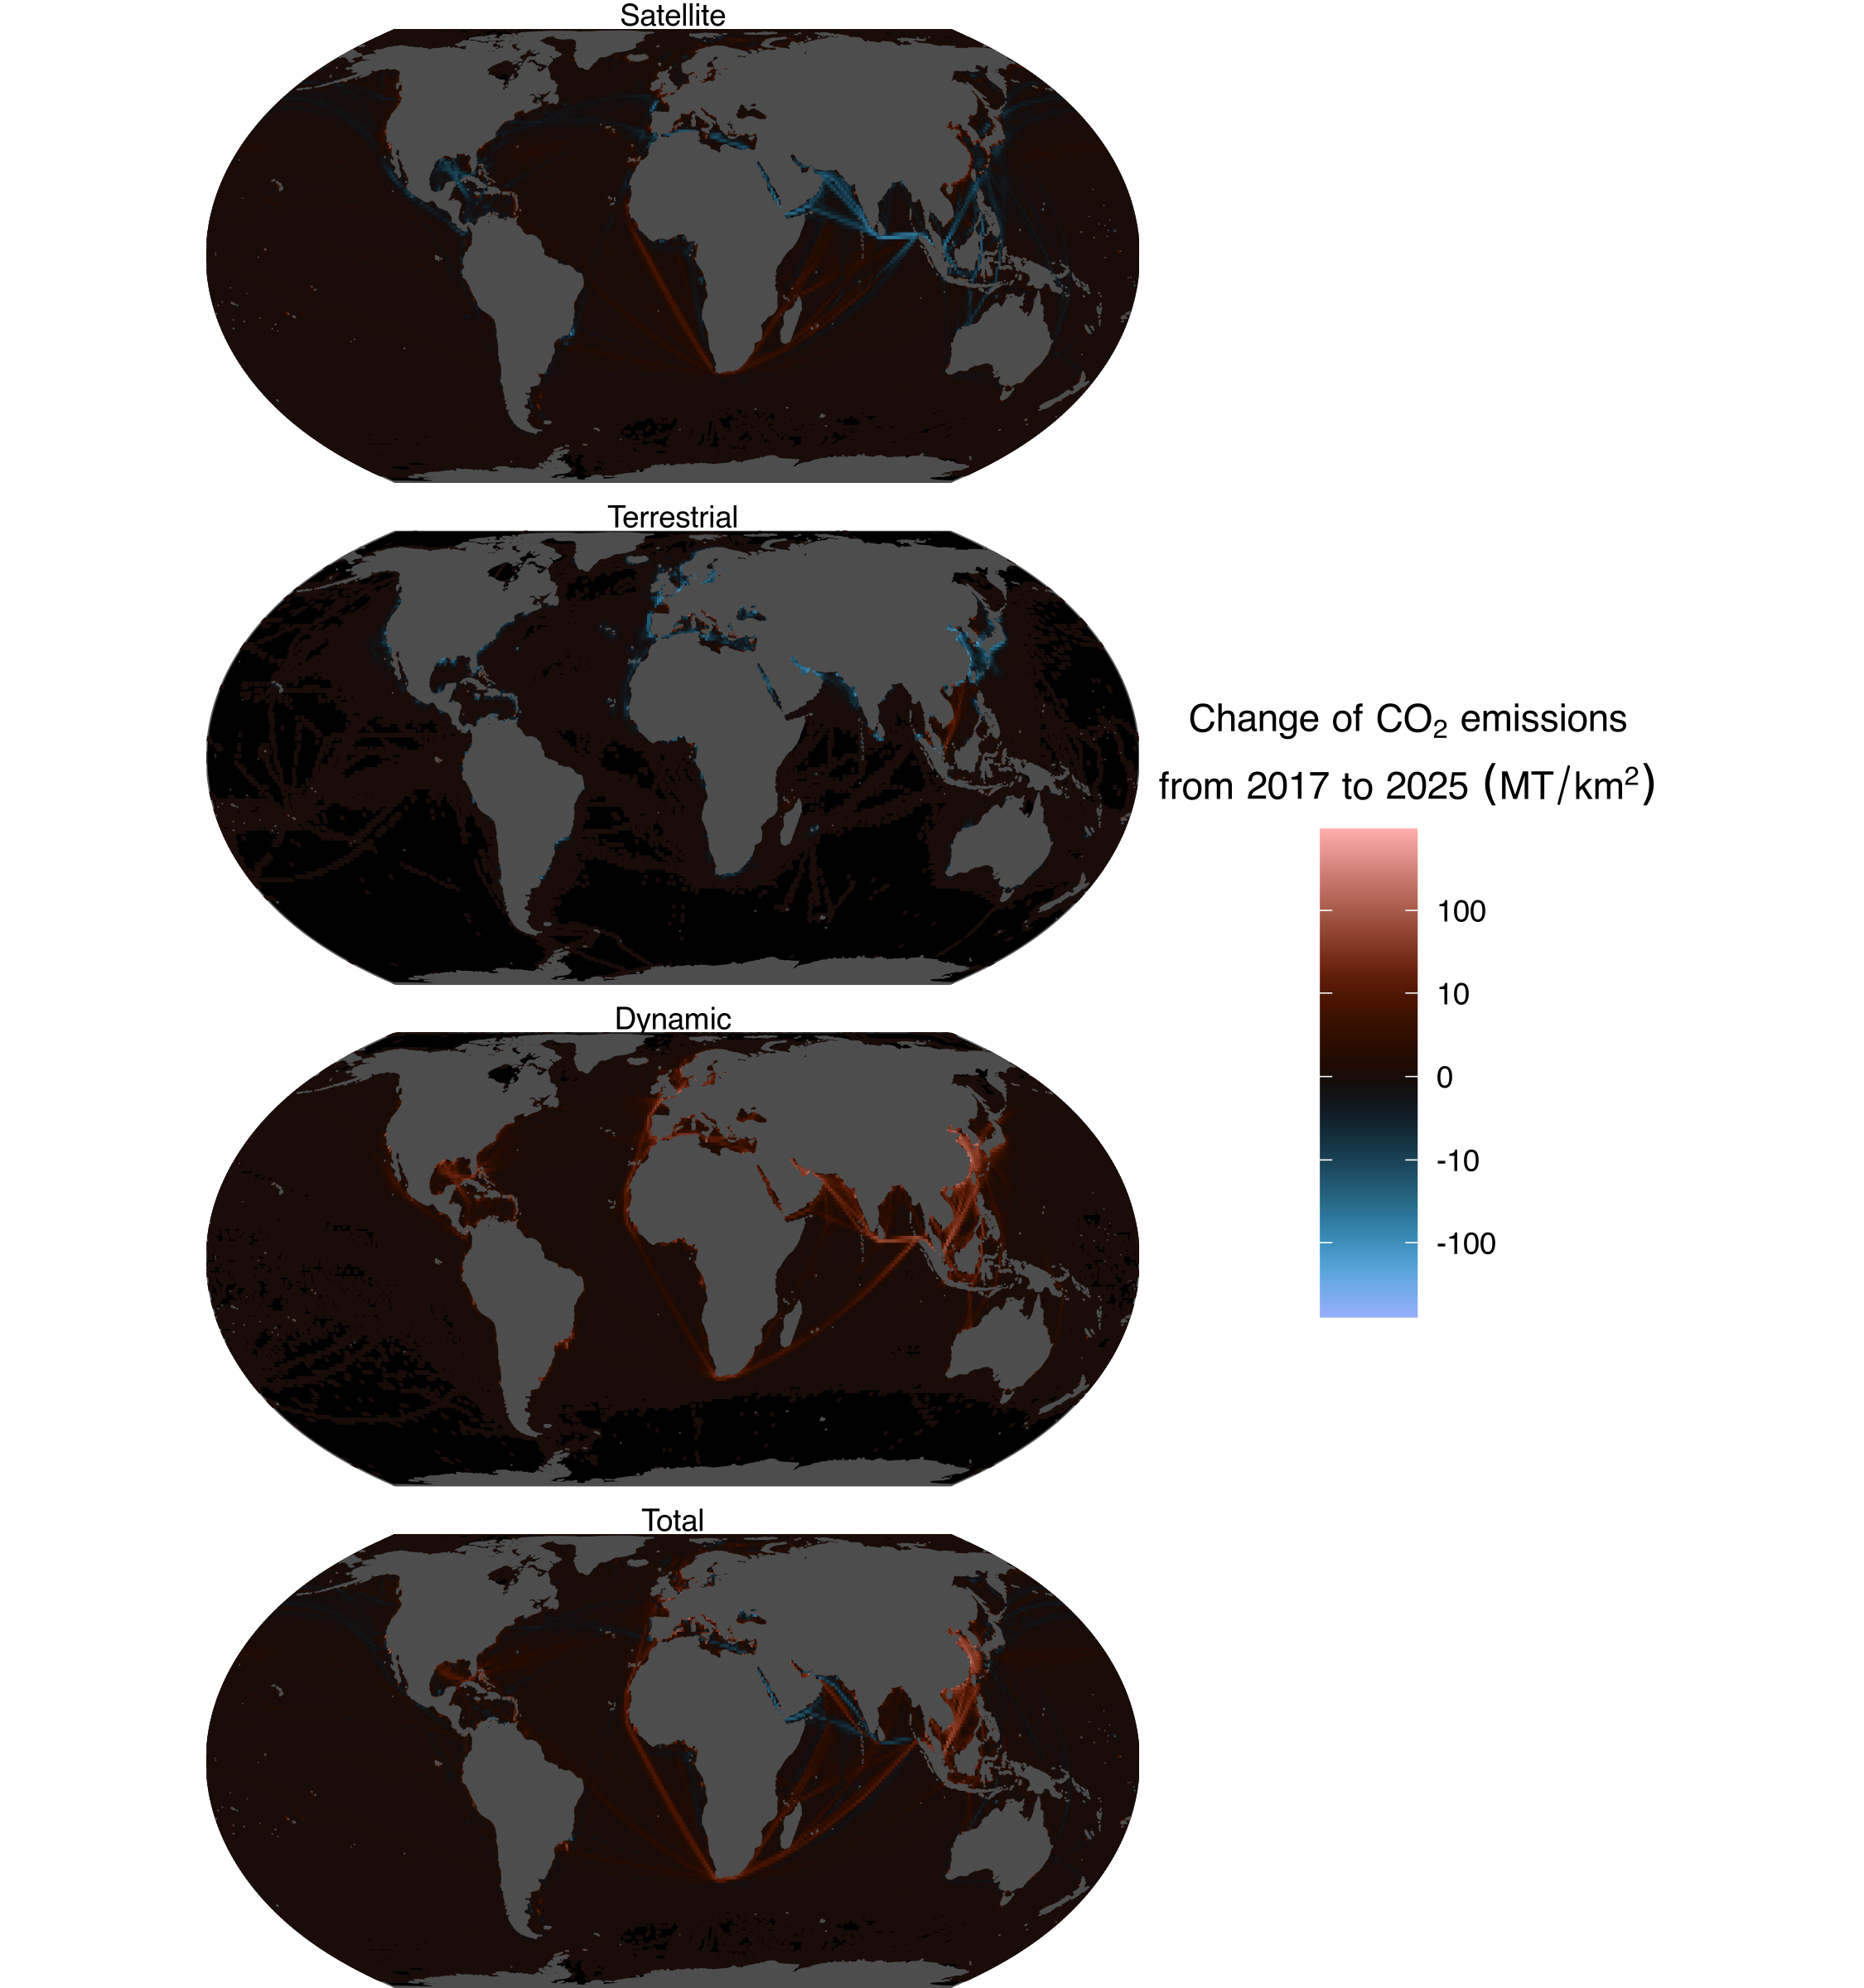
\includegraphics[width=\columnwidth]{figures/fig-co2-emissions-change-map-by-receiver-type-1.png}
    \caption{Spatial change in CO$_{2}$ emissions by AIS-broadcasting vessels between 2017 and \DIFdelbeginFL \DIFdelFL{2024 }\DIFdelendFL \DIFaddbeginFL \DIFaddFL{2025 }\DIFaddendFL (metric tonnes) by receiver type (satellite, terrestrial, and dynamic) and total across receiver types, at a 1x1 degree spatial resolution; emissions are area-normalized for each pixel (metric tonnes per square kilometer, shown on a pseudolog-10 scale).}
    \label{fig:fig-co2-emissions-change-map-by-receiver-type}
\end{figure}
\DIFaddbegin 


\supnote{Systematic comparison of our AIS-based emissions modeling methodology to other AIS-based inventories}{sec:methods-comparison}

\subsubsection*{\DIFadd{Scope of the comparison and modeling approaches}}

\DIFadd{Global vessel emission estimates fall into two methodological families, distinguished by whether emissions are derived from aggregate country-level fuel use statistics (i.e., `top-down') or from the observed activity of individual vessels (i.e., `bottom-up'). Top-down, fuel-based inventories combine reported marine fuel sales with fleet-wide emissions factors, without using data on individual vessels. They are unable to estimate vessel-level emissions or assign emissions with high spatiotemporal precision, and are known to underestimate emissions relative to activity-based inventories \mbox{%DIFAUXCMD
\cite{miolaEstimatingAirEmissions2011}}\hskip0pt%DIFAUXCMD
. Bottom-up, activity-based approaches instead derive emissions mechanistically from the observed movement of individual vessels, calculating the pollutants emitted by each vessel in a specific spatial context and aggregating over time and fleet \mbox{%DIFAUXCMD
\cite{nunesActivitybasedMethodologyAssess2017}}\hskip0pt%DIFAUXCMD
. 
}

\DIFadd{Since the widespread adoption of AIS, which resolves vessel activity and operational mode at high spatial and temporal resolution, bottom-up AIS-based models have become the reference methodology for global inventories and the approach adopted by the IMO \mbox{%DIFAUXCMD
\cite{fourth2020greenhouse}}\hskip0pt%DIFAUXCMD
. We therefore build on an extensive body of work and literature that has been developed over the last several decades. The most recent and representative global bottom-up inventories include:
}

\begin{itemize}
    \item \DIFadd{Ship Traffic Emissions Assessment Model (STEAM) \mbox{%DIFAUXCMD
\cite{jalkanen2009modelling, jalkanenExtensionAssessmentModel2012, bergShipEmissionsSO22012, johanssonGlobalAssessmentShipping2017, majamaki2025improving}
    }\hskip0pt%DIFAUXCMD
}\item \DIFadd{Shipping Emission Inventory Model (SEIM) \mbox{%DIFAUXCMD
\cite{wangShipEmissionsChina2021, yiHighresolutionGlobalShipping2025}
    }\hskip0pt%DIFAUXCMD
}\item \DIFadd{Maritime Transport Environmental Assessment Model (MariTEAM) \mbox{%DIFAUXCMD
\cite{kramelGlobalShippingEmissions2021}
    }\hskip0pt%DIFAUXCMD
}\item \DIFadd{the OECD's latest bottom-up model update (hereafter `OECD') \mbox{%DIFAUXCMD
\cite{clarke2023co2, oecdMaritimeTransportCO2Methodology2025}
    }\hskip0pt%DIFAUXCMD
}\item \DIFadd{the SAVE model developed by the ICCT (hereafter `SAVE') \mbox{%DIFAUXCMD
\cite{olmer2017greenhouse, documentationV2025031Documentation, mao2025greenhouse}}\hskip0pt%DIFAUXCMD
, and
    }\item \DIFadd{the model used for the Fourth IMO GHG Study (`IMO' in figures and tables) \mbox{%DIFAUXCMD
\cite{fourth2020greenhouse}}\hskip0pt%DIFAUXCMD
.
}

\end{itemize}

\DIFadd{In the following sections, we will compare our AIS-based emissions model to each of these existing inventories. Any AIS-based inventory is assembled from four components, and the differences between these components affect the scope, resolution, and accuracy of each inventory. First, the AIS record itself, which determines which vessels and which movements are observed at all. Second, a vessel-characteristics dataset supplying the parameters the model requires. Third, an engine model converting observed speed into instantaneous main engine load, plus assumptions on auxiliary engine and boiler demand. Fourth, fuel consumption and pollutant-specific emission factors, conditioned on engine type, fuel type and the regulation in force at the time and place of the emission. Supplementary Data 1, 2 and 3 compare our methods, input data, and outputs, respectively, against each of the inventories listed above. The inventories also differ in what they make public (Supplementary Data 3): SEIM and OECD publish their emissions datasets openly, STEAM (through the Copernicus Atmosphere Monitoring Service) and SAVE publish aggregated versions, and MariTEAM and the Fourth IMO GHG Study release no inventory dataset. We will release two datasets on the Global Fishing Watch data download portal: monthly AIS-based emissions at 0.1x0.1-degree resolution by flag and vessel type, with emissions of each of the three GHGs and six pollutants, fuel consumption, hours of activity and distance traveled; and monthly S1-unmatched emissions at 1x1-degree resolution for fishing and non-fishing vessels, with emissions of each of the three GHGs and six pollutants. We end with a comparison of how each inventory is validated against external data sources, and what this tells us about the accuracy of each inventory.
}

\subsubsection*{\DIFadd{Activity and vessel-characteristics data}}

\DIFadd{All seven inventories are global in spatial extent, so the differences lie in AIS coverage, fleet size, and temporal coverage rather than in geographic scope (Supplementary Data 2). The inventories diverge substantially in the number of vessels represented. Restricting the comparison to vessels explicitly modeled from observed AIS activity, we model 800,670 unique vessels over 2015--2025 (a wider window, and so a larger fleet, than the 775,358 vessels emitting during the 2017--2025 study period used elsewhere in this paper), an average of 396,221 vessels per year rising from 249,732 in 2015 to 529,848 in 2025. This exceeds the AIS-modeled fleet of the Fourth IMO GHG Study, OECD, SAVE, MariTEAM and SEIM. Our fleet size is only comparable to the STEAM inventory, which reported 376,219 vessels in 2015, exceeding our fleet size for the same year. However, STEAM does not report fleet sizes in subsequent updates, preventing a direct comparison for the later years in which our fleet is larger.
}

\DIFadd{The difference with STEAM is also reflected in the underlying AIS data, which used approximately 7.8 billion AIS positions in 2015, compared with approximately 2.3 billion in our 2015 dataset after data cleaning. Our own message volume increases to approximately 26.6 billion positions by 2025, totaling approximately 125 billion positions over 2015--2025 (an average of 11.4 billion per year), reflecting the expansion of terrestrial and satellite AIS. Among the remaining inventories, SEIM and MariTEAM report lower AIS message volumes, and the others do not indicate message counts. The increase in AIS messages also reflects the differences in the AIS data types available to us. Terrestrial and satellite AIS constitute the core AIS data types. In addition, GFW obtains a data add-on for both class A and class B D-AIS (also marketed as shipborne AIS), released by the data provider Spire since 2022, which further increases the density and coverage of our AIS record. To our knowledge, D-AIS is generally not included in base AIS data products from most providers, and the inventories covering 2022 onward report conventional AIS data types without indicating whether D-AIS is included, so we cannot determine whether the differences arise from the input data or from a lack of reporting. Of the inventories compared, only OECD (2019 onward) and SAVE (2016-2023) extend into the D-AIS era at all; STEAM's update ends in 2021, SEIM in 2021, the Fourth IMO GHG Study in 2018, and MariTEAM is a single-year 2017 inventory. The question of whether D-AIS inflates our recent trend relative to the others therefore applies to two of the six comparisons. 
}

\DIFadd{Temporal coverage differs in extent. STEAM and MariTEAM are single-year inventories (2015 and 2017 respectively), with STEAM subsequently updated through 2021 to account for ambient conditions \mbox{%DIFAUXCMD
\cite{majamaki2025improving}}\hskip0pt%DIFAUXCMD
. SEIM covers 2013 and 2016--2021, the Fourth IMO GHG Study 2012--2018, SAVE 2016--2023, and OECD from 2019 onward. Our use of consistent GFW AIS products, though input density evolves, enables a continuous AIS-based inventory from 2015, and an AIS-based plus S1-unmatched inventory from 2017, to the present without methodological discontinuities.
}

\DIFadd{Every inventory uses official registries as the primary source of vessel characteristics and applies gap-filling where information is unavailable. The differences are in how far the registry is extended and how the remainder is inferred. The simplest filling approaches substitute central tendencies. The OECD restricts to vessels matching between commercial and public registries and imputes from vessel class and size group means \mbox{%DIFAUXCMD
\cite{oecdMaritimeTransportCO2Methodology2025}}\hskip0pt%DIFAUXCMD
, while SAVE fills missing characteristics from average values \mbox{%DIFAUXCMD
\cite{documentationV2025031Documentation}}\hskip0pt%DIFAUXCMD
. STEAM retains some of the within-class variation by replicating the characteristics of a similar vessel already listed in its database \mbox{%DIFAUXCMD
\cite{johanssonGlobalAssessmentShipping2017}}\hskip0pt%DIFAUXCMD
. MariTEAM fills gaps with regression models, though its modeled fleet is restricted to the registered fleet \mbox{%DIFAUXCMD
\cite{kramelGlobalShippingEmissions2021}}\hskip0pt%DIFAUXCMD
, while the Fourth IMO GHG Study applies similar regressions as its primary method and falls back to class and size medians, on a dataset expanded with registered and public datasets \mbox{%DIFAUXCMD
\cite{fourth2020greenhouse}}\hskip0pt%DIFAUXCMD
. Of the published inventories, SEIM is the only one besides ours to describe a more involved machine-learning approach to infer missing vessel characteristics, applied after extending commercial registries with open data \mbox{%DIFAUXCMD
\cite{yiHighresolutionGlobalShipping2025}}\hskip0pt%DIFAUXCMD
. In our vessel information dataset, characteristics are taken from official registries consolidated through extensive prior scraping work \mbox{%DIFAUXCMD
\cite{park2023tracking}}\hskip0pt%DIFAUXCMD
, and where these are unavailable, from inferred characteristics. Building on \mbox{%DIFAUXCMD
\cite{kroodsma2018tracking}}\hskip0pt%DIFAUXCMD
, these are inferred with new machine-learning models trained on registry data, including S\&P Global Market Intelligence's Ships Dataset (Section \ref{sec:vessel-characteristics-models}). This enables the inclusion of a substantially larger number of vessels than most previous studies, reaching a fleet dominated by small domestic and fishing vessels that the more registry-anchored inventories cannot represent.
}

\DIFadd{Finally, the inventories differ in how they treat vessels absent from the AIS feed. STEAM, SEIM and MariTEAM rely exclusively on AIS or port-call data and make no allowance for unobserved activity. OECD, SAVE and the Fourth IMO GHG Study impute activity and emissions for small registered vessels missing from AIS, scaling from explicitly modeled vessels of the same type and size. Neither approach can account for vessels that are absent from both AIS and registries. We instead estimate S1-unmatched emissions, from vessels detected in S1 SAR imagery that cannot be matched to an AIS broadcast, using machine learning and data fusion (Section \ref{sec:non-broadcasting-vessels}), which recovers vessel activity that does not appear in AIS, both for vessels that simply do not carry AIS transponders at all, and also for vessels that carry AIS transponders but whose signal is not received. To our knowledge this is the first global shipping inventory to do so.
}

\subsubsection*{\DIFadd{Engine and emissions model}}

\DIFadd{Every AIS-based inventory estimates the propulsion energy required by the main engine to overcome hull resistance at the observed vessel speed, and the models differ in the resolution at which the components of that resistance are resolved. The literature defines two main modeling approaches: load-based (i.e., SEIM, SAVE, OECD, the Fourth IMO GHG Study, and our study) and resistance-based (i.e., STEAM and MariTEAM). While load-based models are regarded as adequate approximations of more complex methods, resistance-based models are often avoided because of the number of inputs needed. Resistance models require hull parameters, which restricts their applicability to vessels with such documented information in the registries. Imputing class-average hull parameters may be acceptable for fleet-level aggregates and well-defined classes with limited variation in hull design, but performance declines for underrepresented and heterogeneous classes and can substantially alter single-vessel estimates \mbox{%DIFAUXCMD
\cite{brownPowerModelsAverage2019}}\hskip0pt%DIFAUXCMD
. This limitation is particularly relevant because we model a broader fleet dominated by small domestic and fishing vessels, for which hull geometry is often absent or incomplete, and report emissions at a finer resolution, by trip and by vessel. The resistance model's advantage in physical realism would therefore be offset by uncertainty in its inputs. The load-based formulation, by contrast, requires only installed main engine power, design speed, observed speed and a small number of further characteristics that are readily available in registries and can be modeled with confidence where they are not. As in the other load-based models, correction factors are then applied to main engine load. Draft corrections are applied at a lower resolution than in \mbox{%DIFAUXCMD
\cite{fourth2020greenhouse}}\hskip0pt%DIFAUXCMD
, \mbox{%DIFAUXCMD
\cite{documentationV2025031Documentation} }\hskip0pt%DIFAUXCMD
and \mbox{%DIFAUXCMD
\cite{oecdMaritimeTransportCO2Methodology2025}}\hskip0pt%DIFAUXCMD
, as draft is not reliably reported in our AIS records; weather and fouling corrections follow comparable approaches to the other load-based models; and a new correction is introduced to account for fishing activity.
}

\DIFadd{For engine and fuel parameterization, we adapted the methods of the Fourth IMO GHG Study \mbox{%DIFAUXCMD
\cite{fourth2020greenhouse}}\hskip0pt%DIFAUXCMD
, which established the standard assumptions now adopted by most shipping emissions models. Building an expanded activity dataset around a community reference also allows us to attribute differences from existing inventories to fleet coverage and activity representation. Deviations from those methods depended on data availability or the quality of inferred values, but remain in line with other load-based models \mbox{%DIFAUXCMD
\cite{yiHighresolutionGlobalShipping2025, oecdMaritimeTransportCO2Methodology2025, documentationV2025031Documentation}}\hskip0pt%DIFAUXCMD
. Specific fuel oil consumption (SFOC) and the decomposition of emissions into main engine, auxiliary engine and boiler components follow the general consensus across models \mbox{%DIFAUXCMD
\cite{fourth2020greenhouse, yiHighresolutionGlobalShipping2025, oecdMaritimeTransportCO2Methodology2025, documentationV2025031Documentation}}\hskip0pt%DIFAUXCMD
, including the resistance-based ones \mbox{%DIFAUXCMD
\cite{johanssonGlobalAssessmentShipping2017, kramelGlobalShippingEmissions2021} }\hskip0pt%DIFAUXCMD
(Supplementary Data 1). Our approach is more limited in its treatment of fuel types, which are not explicitly modeled because vessel-level fuel type data are unavailable. For a given engine type, SFOC values and emission factors are therefore calculated as the average across the fuel types associated with that engine type. LNG is therefore not included as a fuel type, since we have no way to identify which vessels use it. Our treatment of policy instruments is also narrower than that of some other models, which apply fuel-sulfur and NOx limits geographically within Emission Control Areas (ECAs) \mbox{%DIFAUXCMD
\cite{johanssonGlobalAssessmentShipping2017, yiHighresolutionGlobalShipping2025, fourth2020greenhouse, documentationV2025031Documentation}}\hskip0pt%DIFAUXCMD
; STEAM and SAVE additionally account for technologies such as scrubbers and dual-fuel operation. Our NOx limits are assigned by engine Tier from build year and engine speed but are not resolved spatially by NOx ECA boundaries, and SOx and PM estimates are expected to be biased upward within ECAs, an effect concentrated before 2020, when the difference between ECA and global sulfur limits was largest.
}

\subsubsection*{\DIFadd{Differences in validation}}

\DIFadd{Validation of existing inventories has rested largely on aggregate benchmarking against independent statistics, top-down approaches and against other bottom-up inventories. Our global totals were cross-compared against all six inventories discussed here, and against the multisector EDGAR and CEDS inventories \mbox{%DIFAUXCMD
\cite{guizzardiGlobalUptoDate2025, hoeslyHistorical17502014Anthropogenic2018}}\hskip0pt%DIFAUXCMD
. As for the other models, STEAM benchmarked global fuel use against IEA statistics and the Third IMO GHG Study, modeled maritime transport work against UNCTAD seaborne-trade statistics and regional results against the EMEP inventory. SEIM, which rests entirely on this class of evidence, compares global totals and trends against EDGAR, CEDS and the Fourth IMO GHG Study, with an activity and fleet benchmark against UNCTAD. MariTEAM cross-compares against the Fourth IMO GHG Study for the same year and STEAM3 for a different year. OECD is the most extensive in this respect, benchmarking global totals against IEA and the Fourth IMO GHG Study, fleet activity against UNCTAD, average efficiencies by class and size against IMO for 2018, and country-level results against national Air Emission Accounts for more than 35 countries. SAVE benchmarks aggregated fuel consumption against IMO DCS for vessels of 5,000 GT and above, and the Fourth IMO GHG Study against the Third IMO GHG Study, its own top-down estimates, the ICCT inventory, and global fuel sales reported by the IEA and UNSD.
}

\DIFadd{Although comparing aggregate emissions totals against other inventories can be illustrative, it does not provide information on how well a model can estimate emissions for a particular vessel; this requires comparison against independent }\textit{\DIFadd{vessel-level}} \DIFadd{emissions or fuel use data. We validate against two such datasets: vessel-specific measured fuel consumption for 16,205 unique vessels from S\&P Global Market Intelligence's Ships Dataset, and EU MRV records covering 27,657 vessel-years. To our knowledge, this is the largest vessel-level validation of a global bottom-up shipping inventory. Other validations using in situ measurements include that of the Fourth IMO GHG Study, which compares yearly estimates against 9,739 vessel records in the 2018 EU MRV dataset and additionally draws on engine power and fuel consumption measurements from 94 vessels' Continuous Monitoring Dataset \mbox{%DIFAUXCMD
\cite{fourth2020greenhouse}}\hskip0pt%DIFAUXCMD
. SAVE also validates per-vessel-year carbon intensity against EU MRV \mbox{%DIFAUXCMD
\cite{documentationV2025031Documentation}}\hskip0pt%DIFAUXCMD
. OECD likewise draws on EU MRV, but compares totals aggregated by vessel class rather than by individual vessel \mbox{%DIFAUXCMD
\cite{oecdMaritimeTransportCO2Methodology2025}}\hskip0pt%DIFAUXCMD
. MariTEAM validates modeled engine power against in situ measurements for a single vessel \mbox{%DIFAUXCMD
\cite{kramelGlobalShippingEmissions2021}}\hskip0pt%DIFAUXCMD
. STEAM was validated in earlier versions against a limited sample of in situ measurements \mbox{%DIFAUXCMD
\cite{bergShipEmissionsSO22012}}\hskip0pt%DIFAUXCMD
, and its recent ambient-conditions update validates modeled fuel consumption against 6,445 vessel-year records in the EU MRV data \mbox{%DIFAUXCMD
\cite{majamaki2025improving}}\hskip0pt%DIFAUXCMD
. This last comparison bears directly on the choice of propulsion formulation (i.e., load-based and resistance-based). Applied to an identical fleet and AIS record, resistance-based methods have been reported to yield lower fleet-level CO$_{2}$ than their load-based equivalents \mbox{%DIFAUXCMD
\cite{brownPowerModelsAverage2019}}\hskip0pt%DIFAUXCMD
, but that offset has so far been established only between models, or against limited samples of in situ measurements \mbox{%DIFAUXCMD
\cite{bergShipEmissionsSO22012, kramelGlobalShippingEmissions2021}}\hskip0pt%DIFAUXCMD
. Here the two families, represented by STEAM and our model, are each tested against the same independent benchmark dataset (i.e., EU MRV) and perform comparably, both achieving an R$^{2}$ of approximately 0.8 \mbox{%DIFAUXCMD
\cite{majamaki2025improving}}\hskip0pt%DIFAUXCMD
, supporting our methodological choices and indicating that the load-based formulation as implemented here does not exhibit the systematic upward bias reported by \mbox{%DIFAUXCMD
\cite{brownPowerModelsAverage2019}}\hskip0pt%DIFAUXCMD
.
}


\supnote{Systematic comparison of our emissions magnitude and trend estimates to other inventories}{sec:inventory-comparison}

\DIFadd{Validation against the registered and EU MRV datasets tests the emissions model vessel by vessel, but not whether the modeled fleet is complete, which benchmarking against independent inventories can test. Below we compare the magnitude and the trend of our estimates against the activity-based inventories introduced in Supplementary Note \ref{sec:methods-comparison}, and then against the fuel-statistics-derived inventories EDGAR and CEDS. Each comparison is limited to what each inventory reports publicly.
}

\subsubsection*{\DIFadd{Comparing our estimates with other bottom-up inventories}}

\DIFadd{Over the first years of the study period, our AIS-based estimates agree closely with STEAM, SEIM, MariTEAM, OECD and SAVE, lying within 13\% of each through 2019, but fall 23\% below the Fourth IMO GHG Study in 2017 (Fig. \ref{fig:fig-emissions-inventory-comparison}, panel a, tabulated in Supplementary Table \ref{tab:inventory_comparison_all_sources}). Our fused total, which adds S1-unmatched emissions rather than imputing unobserved vessels, matches the Fourth IMO GHG Study in 2017 (1.06 billion tonnes of CO$_{2}$ in both) and is within 4\% of it in 2018. This closeness in total emissions coexists with substantial disagreement in fleet scope and AIS coverage, among the other inventories as much as between them and ours, so it does not reflect agreement on fleet extent. Rather, all of these inventories rest on a registry-matched core of roughly 45,000-90,000 large vessels that accounts for most emissions \mbox{%DIFAUXCMD
\cite{fourth2020greenhouse, yiHighresolutionGlobalShipping2025, oecdMaritimeTransportCO2Methodology2025, documentationV2025031Documentation, johanssonGlobalAssessmentShipping2017, kramelGlobalShippingEmissions2021}}\hskip0pt%DIFAUXCMD
. In our inventory, registry-matched vessels likewise produced 78\% of AIS-based CO$_{2}$ in 2017 while making up 30\% of broadcasting vessels. Differences in totals therefore reflect how much of the low-information tail of smaller and unregistered vessels each inventory includes, together with the methodological choices described in Supplementary Note \ref{sec:methods-comparison}. Our per-vessel emissions fall within the range of the other models, at 2.3 kt CO$_{2}$ per vessel per year across all broadcasting vessels and 6.08 kt across registry-matched vessels alone, against 2.33 to 7.90 kt for the other inventories (MariTEAM aside, at 20.6 kt), so the differences are in fleet scope rather than in emissions per vessel.
}

\begin{figure}[H]
    \centering
    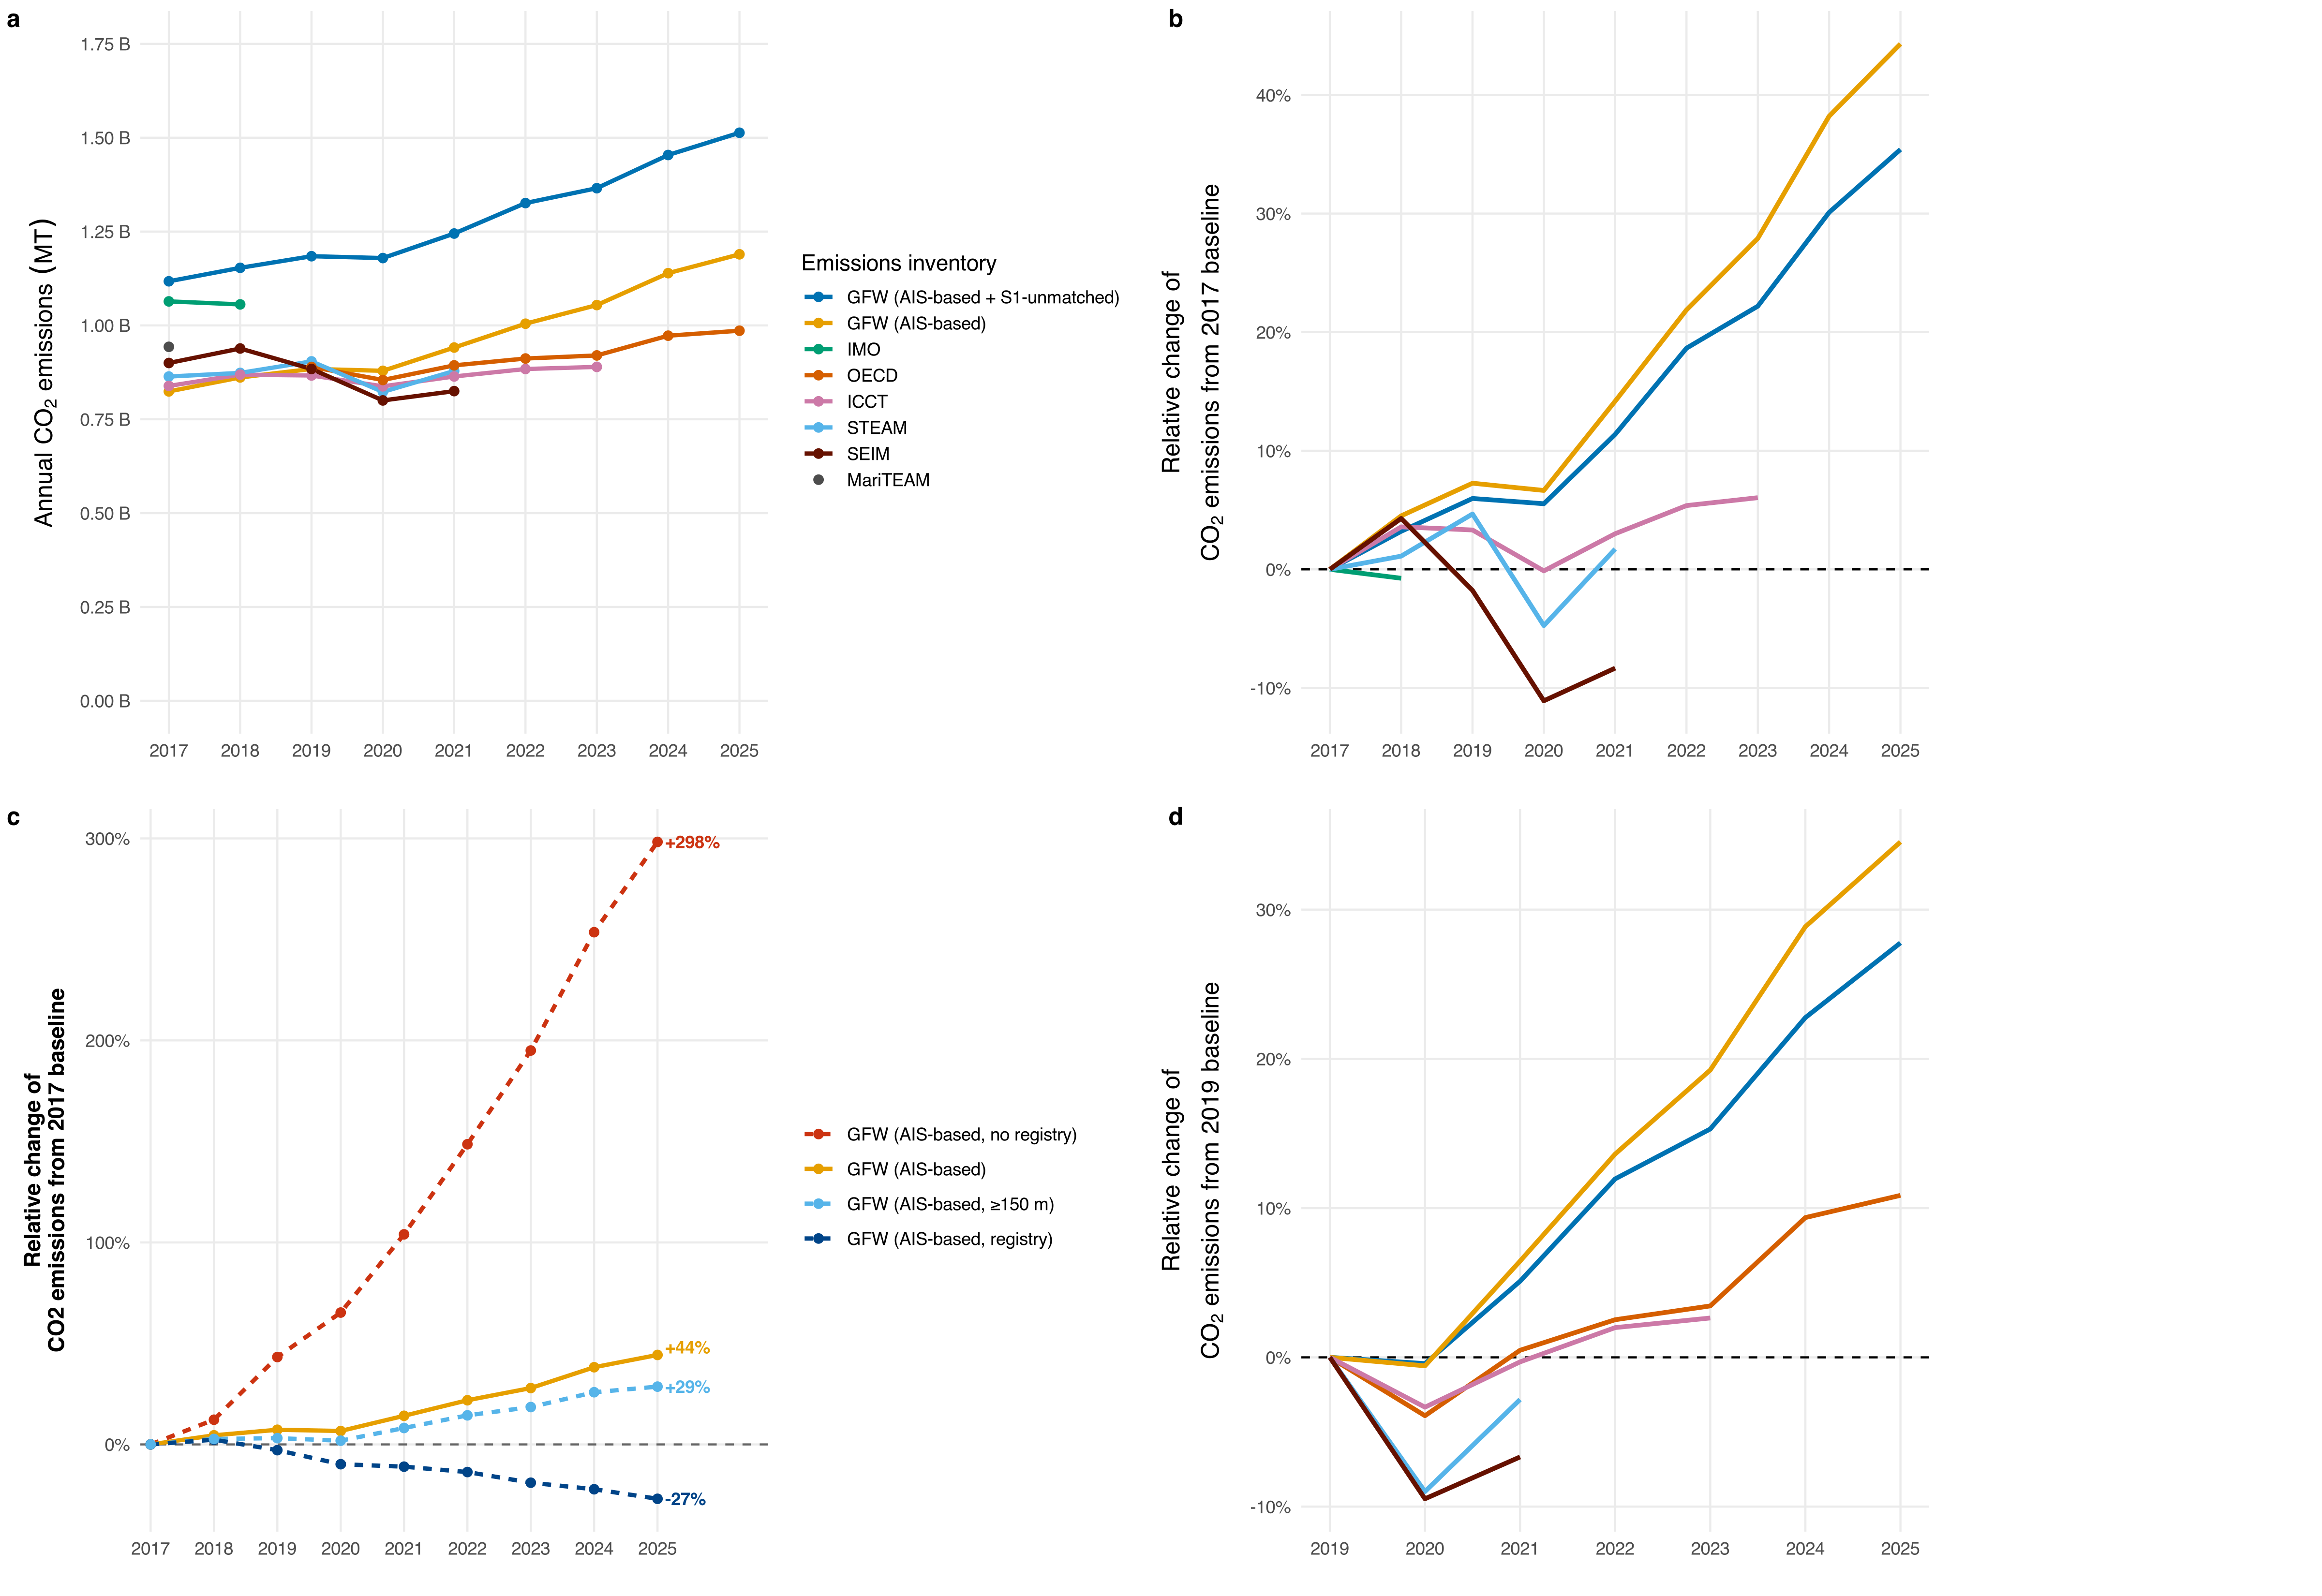
\includegraphics[width=\columnwidth]{figures/figS-inventory-comparison-all-sources-1.png}
    \caption{\DIFaddFL{Trends in our AIS-based and fused estimates against other inventories. (a, b) Change relative to 2017 and to 2019, respectively, against the published bottom-up inventories; the later baseline admits OECD, whose series begins in 2019. (c) Change relative to 2017 against the top-down EDGAR and CEDS inventories, for shipping, all other transportation modes, and all sectors. (d) Our AIS-based series split by vessel length, relative to 2017, using the length bands of Supplementary Table \ref{tab:growth_share_by_family_length}.}}
    \label{fig:figS-inventory-comparison-all-sources}
\end{figure}

%DIF >  Nine columns overflow the text block at the default column padding
\begingroup
\setlength{\tabcolsep}{2.5pt}
\begin{table}[!h]
\centering
\caption{\label{tab:inventory_comparison_all_sources}\DIFaddFL{Annual marine vessel CO$_{2}$ emissions (billions of metric tonnes) for our AIS-based and fused (AIS-based + S1-unmatched) estimates and for the published bottom-up, activity-based inventories. A dash marks a year for which an inventory publishes no estimate.}}
\centering
\fontsize{7}{9}\selectfont
\setlength{\tabcolsep}{3pt}
\begin{tabular}[t]{r|l|l|l|l|l|l|l|l}
\hline
Year & \shortstack{GFW\\(AIS-based +\\S1-unmatched)} & \shortstack{GFW\\(AIS-based)} & IMO & OECD & SAVE & STEAM & SEIM & MariTEAM\\
\hline
2017 & 1.065 & 0.824 & 1.064 & - & 0.839 & 0.864 & 0.900 & 0.943\\
\hline
2018 & 1.098 & 0.861 & 1.056 & - & 0.869 & 0.874 & 0.939 & -\\
\hline
2019 & 1.128 & 0.884 & - & 0.889 & 0.867 & 0.904 & 0.884 & -\\
\hline
2020 & 1.122 & 0.879 & - & 0.855 & 0.838 & 0.823 & 0.800 & -\\
\hline
2021 & 1.187 & 0.941 & - & 0.894 & 0.864 & 0.879 & 0.825 & -\\
\hline
2022 & 1.259 & 1.005 & - & 0.912 & 0.884 & - & - & -\\
\hline
2023 & 1.299 & 1.054 & - & 0.920 & 0.890 & - & - & -\\
\hline
2024 & 1.384 & 1.139 & - & 0.973 & - & - & - & -\\
\hline
2025 & 1.443 & 1.189 & - & 0.986 & - & - & - & -\\
\hline
\end{tabular}
\end{table}
\endgroup
\FloatBarrier

\DIFadd{In the most recent years our AIS-based series grows faster than every other inventory (Supplementary Fig. \ref{fig:figS-inventory-comparison-all-sources}, panels a and b). The difference lies in how the fleets are defined. Inventories constrained by commercial registries change primarily at the pace of registry updates and activity of vessels within the registry, whereas our fleet is defined by AIS observation and grows with AIS carriage. Our broadcasting fleet accordingly grows faster than the OECD and SAVE fleets, the only inventories publishing vessel counts over the recent period, and most of that growth comes from small vessels (Supplementary Table \ref{tab:growth_share_by_family_length}; Supplementary Fig. \ref{fig:figS-inventory-comparison-all-sources}, panel d; Supplementary Fig. \ref{fig:figS-growth-timeline-by-family-length}). Among detected large non-fishing vessels, the segment where AIS carriage is mandated and registry coverage is strongest, the share with no matching AIS broadcast is essentially unchanged since 2017, whereas it falls steeply among small non-fishing and fishing vessels as AIS carriage and reception expand (Supplementary Fig. \ref{fig:figS-ais-carriage-saturation-by-size}). Consistent with this, vessels under 50 m, which are numerous, largely coastal, and poorly covered by registries, contribute the largest share of the growth in our AIS-based series, led by passenger vessels (Supplementary Fig. \ref{fig:figS-passenger-size-panels}), and they enter it mainly as they begin to broadcast: of the 142 million tonne increase from service and passenger vessels under 50 m, 126 million tonnes came from the change in vessel count (Supplementary Table \ref{tab:growth_decomposition_by_family_length}). The phase-in of D-AIS (Supplementary Note \ref{sec:ais-receiver-types}) adds a second, smaller effect: AIS positions received more than doubled between 2021 and 2025 while observed distance traveled and AIS-based emissions rose together by only $\sim$27\%, so D-AIS mostly densified trajectories that were already observed rather than adding new activity. The exception is small fishing vessels: their distance per vessel rose 51\% between 2017 and 2025, accounting for 13 of their 35 million tonne increase, consistent with improved reception tracking vessels that were already broadcasting over more of their activity (Supplementary Table \ref{tab:growth_decomposition_by_family_length}). The divergence from the other inventories therefore suggests that the other inventories, and our own estimates for early years, miss part of the fleet, and that any AIS-based trend partly measures the expansion of AIS carriage rather than of activity at sea. We return to this second point below.
}

\begin{figure}[H]
    \centering
    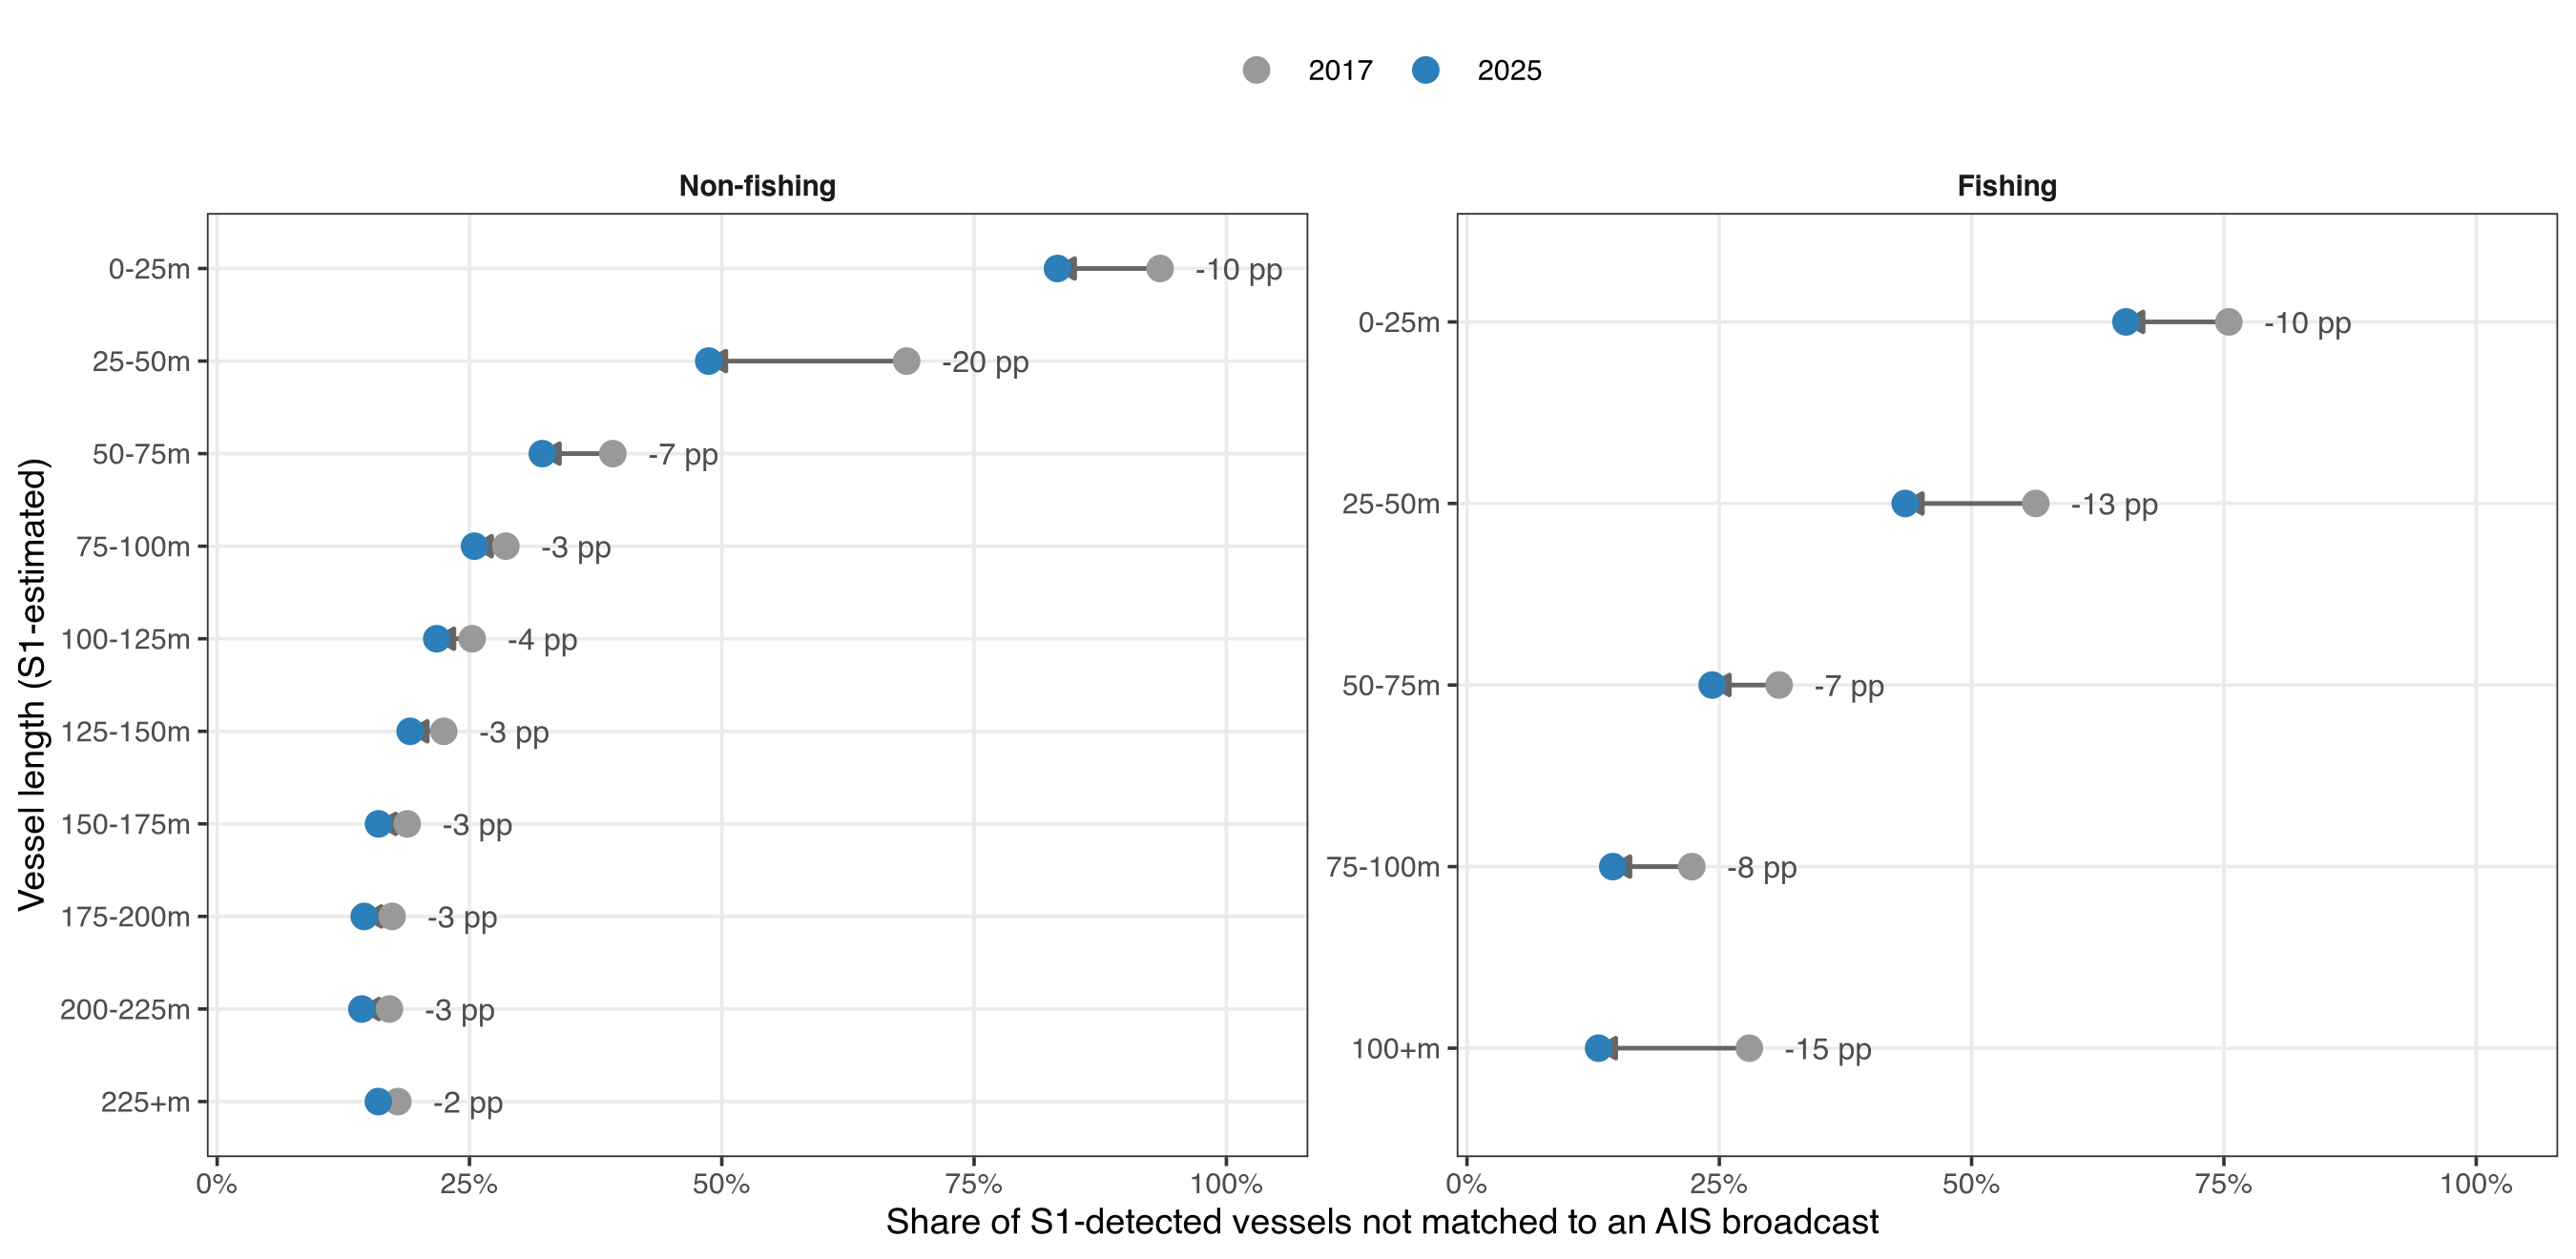
\includegraphics[width=\columnwidth]{figures/figS-ais-carriage-saturation-by-size-1.png}
    \caption{\DIFaddFL{AIS carriage saturation by vessel size: share of S1 detections with no matching AIS broadcast, by length bin, 2017 against 2025. The unmatched share is flat for the largest vessels and falls steeply for the smallest.}}
    \label{fig:figS-ais-carriage-saturation-by-size}
\end{figure}

\DIFadd{Our fused total (AIS-based + S1-unmatched) exceeds every other inventory in every year after 2017 (Fig. \ref{fig:fig-emissions-inventory-comparison}, panel a) because it extends the fleet through satellite imagery-based detections to vessels that appear in neither registries nor AIS. The Fourth IMO GHG Study, OECD, and SAVE also attempt to account for non-broadcasting vessels by assigning small registered vessels without AIS signals the activity profiles of explicitly modeled vessels, yet only the IMO study approaches our total, because this imputation can only add vessels listed in a registry.
}

\subsubsection*{\DIFadd{Comparing our estimates with top-down inventories}}

\DIFadd{We also compared our fused estimates against two inventories derived from fuel statistics, the Emissions Database for Global Atmospheric Research (EDGAR) and the Community Emissions Data System (CEDS). EDGAR builds its shipping estimate from reported fuel sales, representing international shipping from international marine bunkers and domestic activity from domestic navigation fuel statistics, with recent years extrapolated from Energy Institute fuel oil trends \mbox{%DIFAUXCMD
\cite{guizzardiGlobalUptoDate2025}}\hskip0pt%DIFAUXCMD
; it can therefore only count fuel that was sold and reported. CEDS starts from the same fuel statistics but treats them as systematically under-reported and scales its global shipping total to bottom-up estimates, mainly the IMO GHG Studies \mbox{%DIFAUXCMD
\cite{hoeslyHistorical17502014Anthropogenic2018, ceds_data_and_assumptions}}\hskip0pt%DIFAUXCMD
, so it also inherits the fleet-scope limits described above. Our fused total exceeds both (Fig. \ref{fig:fig-emissions-inventory-comparison}, panel b, tabulated in Supplementary Table \ref{tab:multisector_shipping_comparison}). The gap in magnitude and the gap in trend have different causes.
}

\begin{table}[!h]
\centering
\caption{\label{tab:multisector_shipping_comparison}\DIFaddFL{Annual marine vessel CO$_{2}$ emissions (billions of metric tonnes) for our AIS-based and fused (AIS-based + S1-unmatched) estimates against the shipping sector of the top-down EDGAR and CEDS inventories, whose shipping scope combines international and domestic navigation. A dash marks a year for which an inventory publishes no estimate.}}
\centering
\fontsize{8}{10}\selectfont
\begin{tabular}[t]{r|l|l|l|l}
\hline
Year & \shortstack{GFW\\(AIS-based +\\S1-unmatched)} & \shortstack{GFW\\(AIS-based)} & EDGAR - Shipping & CEDS - Shipping\\
\hline
2017 & 1.065 & 0.824 & 0.881 & 1.040\\
\hline
2018 & 1.098 & 0.861 & 0.887 & 1.031\\
\hline
2019 & 1.128 & 0.884 & 0.875 & 1.030\\
\hline
2020 & 1.122 & 0.879 & 0.798 & 0.937\\
\hline
2021 & 1.187 & 0.941 & 0.833 & 0.979\\
\hline
2022 & 1.259 & 1.005 & 0.837 & 0.975\\
\hline
2023 & 1.299 & 1.054 & 0.890 & 1.014\\
\hline
2024 & 1.384 & 1.139 & 0.860 & -\\
\hline
2025 & 1.443 & 1.189 & - & -\\
\hline
\end{tabular}
\end{table}
\FloatBarrier

\begin{table}[!h]
\centering
\caption{\label{tab:inventory_growth_comparison}\DIFaddFL{Growth in CO$_2$ emissions for our estimates and for every inventory compared in Supplementary Note \ref{sec:inventory-comparison}. All series are anchored at 2017 where they extend that far back, and because the inventories end in different years each is summarized to its own end year. Growth is reported two ways: the total percent change between the first and last year, and the compound annual growth rate (CAGR). The Fourth IMO GHG Study ends in 2018 and is therefore reported over its native 2015-2018 window, since anchoring it at 2017 would leave a single year-on-year change. MariTEAM is a single-year inventory and admits no growth rate. EDGAR and CEDS changes are shown for All sectors, Other transportation and Shipping scopes.}}
\centering
\fontsize{8}{10}\selectfont
\begin{tabular}[t]{l|c|r|r}
\hline
Series & Time window & Total \% change & CAGR (\%/yr)\\
\hline
\multicolumn{4}{l}{\textbf{Ours}}\\
\hline
\hspace{1em}GFW (AIS-based + S1-unmatched) & 2017--2025 & +35.52 & +3.87\\
\hline
\hspace{1em}GFW (AIS-based) & 2017--2025 & +44.31 & +4.69\\
\hline
\hspace{1em}GFW (AIS-based, $\geq$150 m) & 2017--2025 & +28.62 & +3.20\\
\hline
\multicolumn{4}{l}{\textbf{Bottom-up}}\\
\hline
\hspace{1em}IMO & 2015--2018 & +6.56 & +2.14\\
\hline
\hspace{1em}OECD & 2019--2025 & +10.85 & +1.73\\
\hline
\hspace{1em}SAVE & 2017--2023 & +6.04 & +0.98\\
\hline
\hspace{1em}STEAM & 2017--2021 & +1.71 & +0.42\\
\hline
\hspace{1em}SEIM & 2017--2021 & -8.33 & -2.15\\
\hline
\hspace{1em}MariTEAM & 2017 & --- & ---\\
\hline
\multicolumn{4}{l}{\textbf{EDGAR}}\\
\hline
\hspace{1em}All sectors & 2017--2024 & +7.06 & +0.98\\
\hline
\hspace{1em}Other transportation & 2017--2024 & +3.35 & +0.47\\
\hline
\hspace{1em}Shipping & 2017--2024 & -2.38 & -0.34\\
\hline
\multicolumn{4}{l}{\textbf{CEDS}}\\
\hline
\hspace{1em}All sectors & 2017--2023 & +5.60 & +0.91\\
\hline
\hspace{1em}Other transportation & 2017--2023 & +3.27 & +0.54\\
\hline
\hspace{1em}Shipping & 2017--2023 & -2.46 & -0.41\\
\hline
\end{tabular}
\end{table}
\FloatBarrier

\DIFadd{The magnitude gap arises from three differences in the fleets these inventories can account for. First, fishing largely falls outside the shipping sector in both. They report fishing fuel combined with agriculture and forestry, so EDGAR's shipping estimate contains no fishing vessels at all, while in CEDS only some unreported fishing fuel is absorbed into global shipping through the bottom-up anchor. Second, small coastal and inland vessels are only partly covered: domestic navigation fuel is intended to capture this traffic, but the sector is inconsistently defined across reporting countries \mbox{%DIFAUXCMD
\cite{kuenen2014tno}}\hskip0pt%DIFAUXCMD
. Third, neither inventory can capture fuel that never passes through reported channels, affecting vessels supplied informally or illegally. Each of these mechanisms adds emissions that the top-down inventories omit, and our own detection limits mean that we likely understate the total further.
}

\DIFadd{The trend gap is different in kind. Growth in our AIS-based series partly reflects expanding AIS carriage and coverage, as shown above. The fused total should be less sensitive to that: a vessel that adopts AIS and begins to broadcast moves from the S1-unmatched component to the AIS-based one, reallocating emissions between them rather than adding to the total. In principle, therefore, increases in the fused total should reflect new activity rather than changes in AIS coverage. S1 detections, which depend on neither AIS broadcasting nor registration, offer a partial check on that. Detected activity per observed area stayed roughly flat overall, but its composition shifted, growing among small non-fishing vessels and, most strongly, among the largest, while mid-size classes were flat and fishing declined (Supplementary Fig. \ref{fig:figS-density-by-match-status}, panel a). For the largest non-fishing vessels, AIS carriage is already near-universal and the unmatched share has barely changed since 2017 (Supplementary Fig. \ref{fig:figS-ais-carriage-saturation-by-size}), so their growth must largely reflect new activity; because a large ship can emit on the order of a hundred times what a smaller one does, that compositional shift pushes the emissions trend upward.
}

\begin{figure}[H]
    \centering
    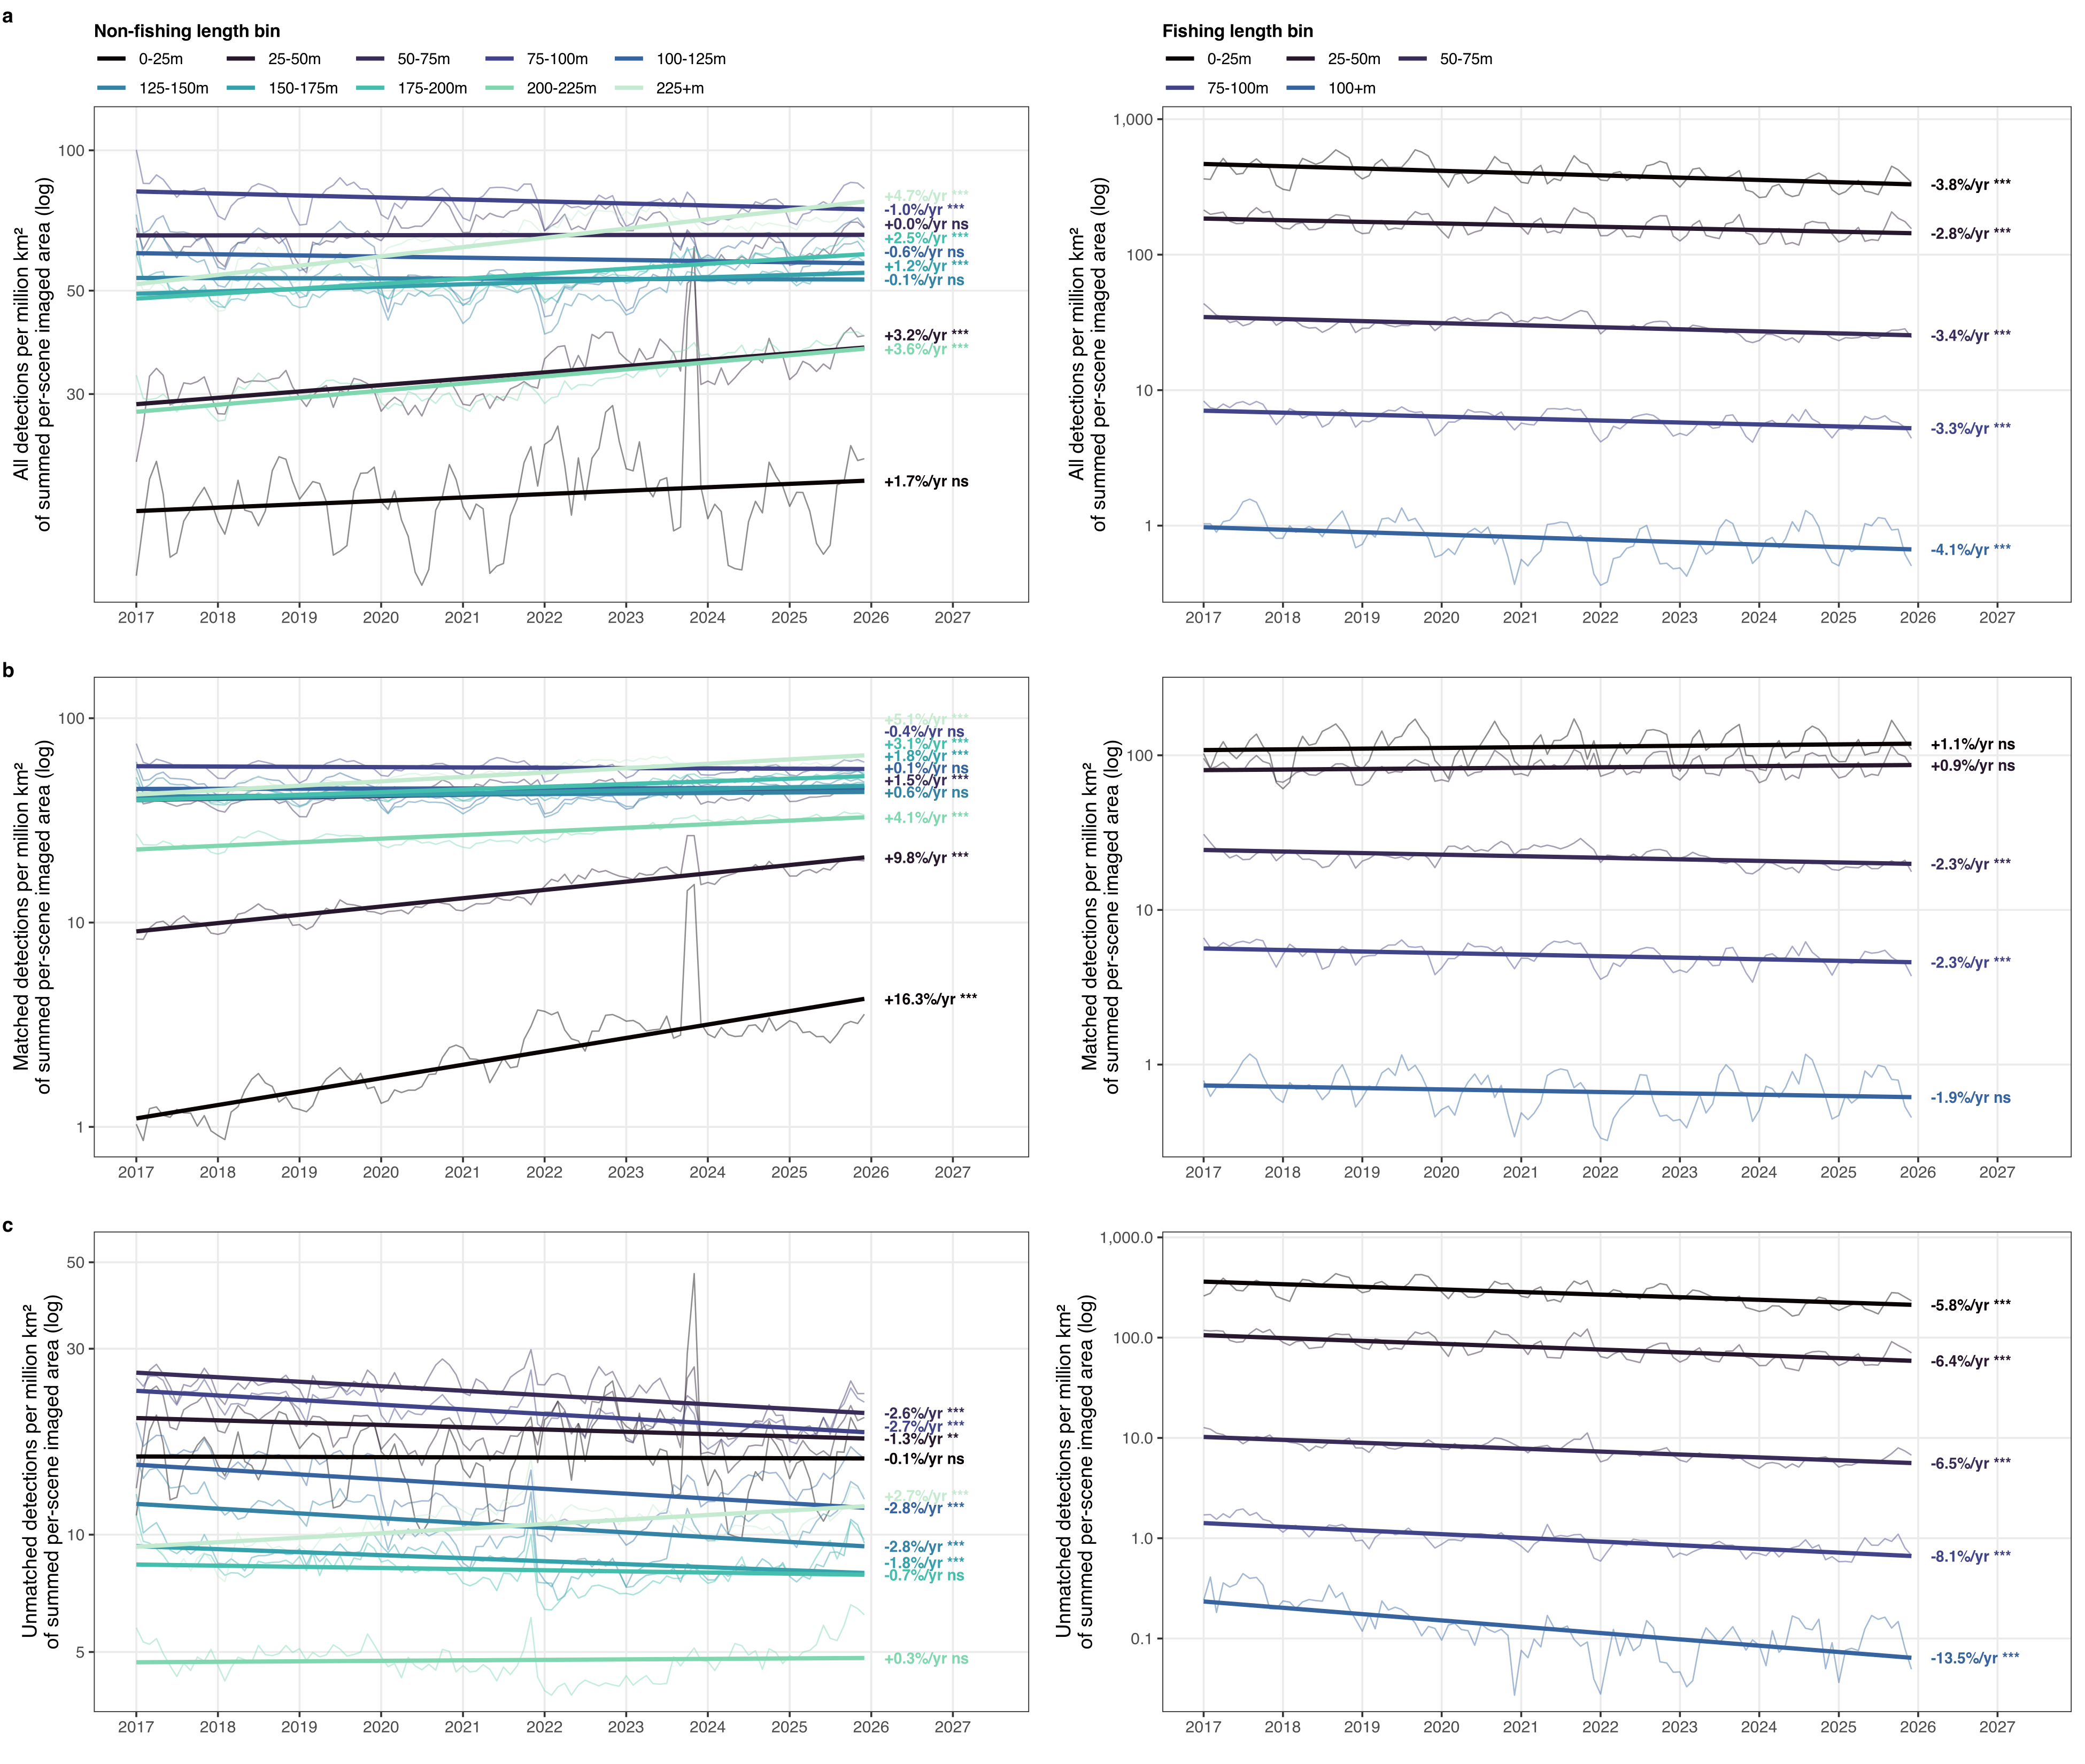
\includegraphics[width=\columnwidth]{figures/figS-density-by-match-status-1.png}
    \caption{\DIFaddFL{S1 detection density by length bin, split into total, AIS-matched and unmatched detections, for fishing and non-fishing fleets, 2017--2025. Density is expressed per unit of S1 sampling effort on the same measure our emissions models use to normalize their detection features (detections per 10\textsuperscript{6} km² of per-scene imaged area summed across scenes), so the three series share a denominator and are additive. Axes are log scaled. Thin lines are monthly values; thick lines are ordinary least squares fits of log density on time over the full period, labeled with the fitted trend in percent change per year and its significance from the slope's two-sided $t$ test (*** $p<0.001$, ** $p<0.01$, * $p<0.05$, ns otherwise).}}
    \label{fig:figS-density-by-match-status}
\end{figure}

\DIFadd{Reallocation between our components, however, holds only where S1 had already detected the vessel. Vessels too small or too close to shore to be reliably detected contribute nothing to the S1-unmatched component and enter the fused total for the first time when they begin broadcasting. Because AIS carriage and reception expanded over the study period, that unobserved fraction was larger at the start of the series than at the end, so part of the measured growth in the fused total can be that gap closing rather than activity rising. The fact that our fused trend closely tracks the AIS-based trend, only slightly shallower at 36\% against 44\% growth between 2017 and 2025, is consistent with this: some genuine reallocation and new activity occur, but part of the measured growth may enter directly through AIS adoption. This could bias our estimated growth trend upward relative to the true trend in activity, even in our fused estimates. However, this does not necessarily mean that the near-flat trends reported by other inventories are accurate either. The reconciliation comes from the part of the fleet our approach captures most completely, non-fishing vessels of 150 m and above, where AIS carriage was already saturated at the start of our series (Supplementary Fig. \ref{fig:figS-ais-carriage-saturation-by-size}). AIS-based emissions from this segment still rose 29\% between 2017 and 2025 (Supplementary Fig. \ref{fig:figS-inventory-comparison-all-sources}, panel d), and that growth came through the number of vessels rather than through distance per vessel, which is where improved reception would show (Supplementary Table \ref{tab:growth_decomposition_by_family_length}). S1-unmatched emissions are not disaggregated by vessel size, so we cannot give a fused figure for this segment separately. The growth that remains once observational expansion is set aside is thus lower than our headline figure, but still well above the near-flat trends of the other inventories: even confined to this segment of large non-fishing vessels, AIS-based emissions grew at a compound annual rate of 3.20\%, only 0.67 percentage points below the 3.87\% growth rate of our fused total emissions. This is still nearly twice that of OECD (1.73\%/yr), the fastest-growing bottom-up inventory that extends beyond 2018, more than three times that of global emissions across all sectors, and about six to seven times that of all other transportation modes combined (Supplementary Fig. \ref{fig:figS-inventory-comparison-all-sources}, Supplementary Table \ref{tab:inventory_growth_comparison}).
}\DIFaddend 

\end{document}
